\documentclass[11pt]{book}
\usepackage{graphicx,epic,fancybox,curves,fancybox,makeidx}
%%% displayed synchronous programs
\makeatletter
\def\BEP{\begin{trivlist}\item[]
  \if@minipage\else\vskip\parskip\fi
  \leftskip\@totalleftmargin \advance\leftskip by 1\parindent
  \rightskip\z@ \parindent\z@ \parfillskip\@flushglue \parskip\z@
  \@tempswafalse \def\par{\if@tempswa\hbox{}\fi\@tempswatrue\@@par}
  \obeylines \tt \small \catcode``=13 \@noligs\frenchspacing\@vobeyspaces}
\def\EEP{\end{trivlist}}
\makeatother

\def\pp#1{\texttt{\small{#1}}}
\newcommand{\PP}[1]{\noindent{\textit{\textbf{#1}}}}

\def\X#1{$x_{#1}$}
\def\B#1{\texttt{#1}}

\def\se{\textit{syn{\small ERJY}}}
\def\sec{\textit{syn{\small ERJYcharts}}}
\def\sef{\textit{syn{\scriptsize ERJY}}}
\def\argos{\textsc{Argos}}
\def\lustre{\textsc{Lustre}}
\def\signal{\textsc{Signal}}
\def\esterel{\textsc{Esterel}}
\def\statecharts{\textsc{Statecharts}}
\def\synccharts{\textsc{SyncCharts}}
\def\java{\textsc{Java}$^{\mbox{\tiny TM}}$}
\def\matlab{\textsc{MATLAB}$^{\mbox{\tiny TM}}$}

\newcommand{\GO}[0]{{\small GO}}
\newcommand{\GOs}[0]{{\small GO}s}
\newcommand{\spc}[0]{\vspace{0.2cm}}

\newcommand{\vs}[0]{\vspace{1pt}}
\newcommand{\NTI}[1]{\textit{#1}}
\newcommand{\NTD}[1]{{\em #1}\label{#1}}
\newcommand{\NT}[1]{\index{#1@{\em #1}}\hyperref{#1}{#1}{}{#1}}
\newcommand{\NTZ}[2]{\index{#1@{\em #1}}\hyperref{#1}{#1#2}{}{#1}}
\newcommand{\KWI}[1]{{\index{#1@{\tt #1}}\tt #1}}
\newcommand{\T}[1]{{\tt #1}}
\newcommand{\is}[0]{$\Rightarrow$\vs}
\newcommand{\mto}[0]{$\mapsto$}
\newcommand{\Bopt}[0]{{\bf (}}
\newcommand{\optE}[0]{{\bf )\opt}}
\newcommand{\opt}[0]{$_{\textit{\scriptsize opt~}}$}
\newcommand{\Balt}[0]{{\bf (}}
\newcommand{\alt}[0]{\,$|$}
\newcommand{\altE}[0]{{\bf )$_\mbox{\em alt~}$}}
\renewcommand{\altE}[0]{{\bf )~}}
\newcommand{\lst}[0]{{...~~}}
\newcommand{\lsep}[1]{...\fbox{\scriptsize #1}...~~}
\newcommand{\rr}[0]{\vs\makebox[7mm]{}}

\newtheorem{example}{\bf Example}[section]
\newenvironment{BNF}{}{}

\def\codeinput#1{\IfFileExists{../tex_input/se.#1}{\input ../tex_input/se.#1}{\begin{center}chpt\_\thechapter\_#1.se\end{center}} {\footnotesize(cf. \texttt{chpt\_\thechapter\_#1.se})}}

\def\codefragment#1{\IfFileExists{../tex_input/se.#1}{\input ../tex_input/se.#1}{\begin{center}chpt\_\thechapter\_#1.se\end{center}}}

\def\codeinputref#1{\IfFileExists{../tex_input/se.#1}{\input ../tex_input/se.#1}{\begin{center}ref\_#1.se\end{center}} {\footnotesize(cf. \texttt{ref\_#1.se})}}

\def\codeinputuser#1{\IfFileExists{../tex_input/se.#1}{\input ../tex_input/se.#1}{\begin{center}user\_#1.se\end{center}} {\footnotesize(cf. \texttt{user\_#1.se})}}

\def\A{\mbox{${\cal A}$}}
\def\C{\mbox{${\cal C}$}}
\def\D{\mbox{${\cal D}$}}
\def\E{\mbox{${\cal E}$}}
\def\F{\mbox{${\cal F}$}}
\def\H{\mbox{${\cal H}$}}
\def\I{\mbox{${\cal I}$}}
\def\L{\mbox{${\cal L}$}}
\def\M{\mbox{${\cal M}$}}
\def\P{\mbox{${\cal P}$}}
\def\Q{\mbox{${\cal Q}$}}
\def\R{\mbox{${\cal R}$}}
\def\S{\mbox{${\cal S}$}}
\def\V{\mbox{${\cal V}$}}

\def\ARROW#1#2{\mbox{\def\arraystretch{0.1}\begin{tabular}{c}
$\ \scriptstyle #1\ $\\
\rightarrowfill\\
$\ \scriptstyle #2\ $\end{tabular}}}

\def\mkTitle#1{
\title{
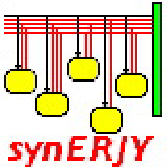
\includegraphics[height=50pt]{../pdf/se-logo}\hspace{0.5cm}
{\Huge \textit{\textbf{synERJY} 5.3}} \\ \vspace{1cm}\
       \textbf{#1}}

\author{\textit{Reinhard Budde}\\
\textit{Axel Poign\'e}\\
\textit{Karl-Heinz Sylla}\\
\ \\
\textbf{Fraunhofer Institut}\\\ \\ 
\textbf{Autonome intelligente Systeme}\\\ \\
\textbf{Fraunhofer AiS}\\\ \\\ \\
\\\ \\\ 
\\\  \\\ \\\ \\\ \\\ \\\textbf{\Large }
}

\date{\today}
}

\makeindex

%\includeonly{semantics}

\mkTitle{An Introduction to the Language}

\begin{document}

\maketitle


\section*{Preface}

\se\footnote{\sef\ may be read as \textbf{syn}chronous
\textbf{e}mbedded \textbf{r}eactive \textbf{J}ava with a \textbf{y}
for the sound.} is a programming language and a design environment for
embedded reactive systems that combines two paradigms:
\begin{itemize}
    \item \emph{Object-oriented modelling} for a robust and flexible
    design.
      
    \item \emph{Synchronous execution} for precise modelling of
    reactive behaviour.
\end{itemize}
Highlights are that
\begin{itemize}
\item \se\ provides a deep embedding of the reactive behaviour into
      the object-oriented data model.
\item \se\ offers fine-grained integration of synchronous formalisms
      such as \esterel~\cite{esterel}, \lustre~\cite{lustre}, and
      \statecharts~\cite{statecharts}.\footnote{We recommend Halbwachs' book
      \emph{Synchronous Programming of Reactive Systems}~\cite{halbwachs} as 	an excellent introduction.}
\end{itemize}

The programming environment supports compilation, configuration,
simulation, and testing, as well as verification by model checking. 
Behavioural descriptions may be edited in graphical or in textual
form.  Code generators for efficient and compact code in C and several
hardware formats are available.

The \se\ language and its programming environment are developed
at the Fraunhofer Institut Autonome Intelligente Systeme.\footnote{The
development of \sef\ has been partially supported by the ESPRIT LTR
SYRF, ``Synchronous formalisms'', and the ESPRIT IIM Project CRISYS,
``Critical Systems and Instrumentation''.}  The programming
environment is freely available with a public domain license.
\newline

\noindent Contact:  
{\tt\small \{reinhard.budde,poigne,sylla\}@ais.fraunhofer.de}.



\newpage
\section*{Acknowledgements}

We are grateful to all our former colleagues Agathe Merceron, Leazek 
Holenderski, Olivier Maffeis, Matthew Morley, Monika M\"ullergburg, 
Micele Pinna who substantially contributed to the genesis of \se\ 
(as outlined in the Appendix \ref{genesis}).

Further we sincerly thank Albert Benveniste, Paul Caspi, Gerard Berry, Nicholas Halbwachs for being the ``founding fathers'' of synchronous programming, and
for their co-operation and inspiration in the many activities we shared.

\tableofcontents

\chapter{Introduction}

\paragraph{A priori.} Synchronous Programming is a branch of
concurrent programming\index{concurrency}. 
Concurrent programs are inherently more
difficult to write and to debug than sequential programs.  The
sequential execution of each of the parallel branches is interlocked
with communications between the parallel branches, resulting in a
partial order according to which elementary statements are executed. 
Whether such a partial order is explicitly specified by the programmer
(for instance using threads and synchronisations) or automatically
scheduled by a compiler as in case of synchronous languages, the
programmer will sometimes be surprised by unexpected behaviour.  This
one should keep in mind before getting despaired debugging a
concurrent program.

\section{Systems, Models, and Programming}

\paragraph{Models of physical systems.} In the real world we encounter
physical objects such as cars, electronic circuits, power stations,
dogs, space ships, and computer programs.  We refer to these as
\emph{physical systems}\index{system!physical}.

If we start to think about one of these objects we formulate a
\emph{model}\index{system!model} of the object focusing
 upon some small number of
properties we believe sufficient for capturing the behaviour we care
about.  If we wish to analyse the model we need some formal
(mathematical) representation of it.

We may start by considering a system as a black box into which we feed
inputs and out of which we receive outputs, inputs and outputs being
properties we care about.  It is quite common to refer to these
properties as \emph{signals}\index{signal} if we enter into the
mathematical analysis of a system.  In general we cannot expect the
outputs to be completely determined by the inputs, but rather to
depend as well on a set of (internal) properties we refer to as a
\emph{state}\index{system!state}.  A state is some compact
representation of the past activity of the system complete enough to
predict, on the basis of the inputs, exactly what the output will be,
and also to update the state itself.
\begin{center}
       {\tt\scriptsize
       \thinlines
       \setlength{\unitlength}{0.9pt}
       \begin{picture}(210,60)
       \put(15,35){input $u(t)$}
       \put(0,30){\vector(1,0){70}}
       \put(15,20){at time $t$}
       \put(15,10){$u(t) \in U$}
       \put(70,0){\framebox(90,60){}}
       \put(98,10){$x(t) \in X$}
       \put(93,35){state $x(t)$}
       \put(95,25){at time $t$}
       \put(175,35){output $y(t)$}
       \put(175,20){at time $t$}
       \put(175,10){$y(t) \in Y$}
       \put(160,30){\vector(1,0){70}}
      \end{picture}
   }
\end{center}

\paragraph{Time scales.} Given that we have decided what the sets of
input, output and state variables are for our model, we must now
determine on what \emph{time scale} we shall analyse the system.  For
many physical systems we may think of input, output and state as
changing continuously, then a model becomes a \emph{continuous-time
system}\index{system!continuous time}.

On the other hand, a continuous-time model of a computer system is
inappropriate, and we treat them as a \emph{discrete-time
system}\index{system!discrete time}, since we can make only finitely
many measurement at any time interval.  Further, if we use a computer
to control the behaviour in a desired way, we can generate distinct
control signals only at discrete times.

\paragraph{Analyzing systems.} Having modelled a physical system, the
question arises whether we can \emph{control}\index{control} a system
in a given state, providing inputs to bring it into its resting state,
or, given that a system is in its resting state, can we apply inputs
to which will force it to \emph{reach}\index{reachability} a desired
state.  The complimentary question is whether we can
\emph{observe}\index{observability} an unknown state of a system in
such a way as to determine what the state was.  In other words, we
want to analyse the dynamic behaviour of a system.  The differential
and integral calculus provide the main tools for continuous-time
systems, whereas algebra is the main tool for the analysis of
discrete-time systems.  Textbooks provide a vast body of material to
deal with these questions.

All this contributes to the central task of \emph{control
theory}\index{control!theory} of controlling a system to behave in a
desired way.  We have to answer questions such as whether we are able
to control a system at all, or further, if we are able to control a
system in some optimal way, for instance spending a minimal amount of
energy.

\paragraph{System control.} Monitoring a system's performance,
comparing it with some desired reference performance, and using any
discrepancy to generate a correction input to control the system to
approximate the reference, is fundamental pervading all aspects of
modern life.  This is what \emph{feedback
control}\index{control!feedback}\index{feedback} is about
\begin{center}
   {\tt\scriptsize
       \thinlines
       \setlength{\unitlength}{0.75pt}
       \begin{picture}(210,105)
         \put(5,85){$u(t)$}
         \put(0,80){\vector(1,0){60}}
         \put(60,60){\framebox(90,40){plant}}
         \put(190,85){$y(t)$}
         \put(150,80){\vector(1,0){60}}
         \put(60,0){\framebox(90,40){controller}}
         \put(30,20){\line(1,0){30}}
         \put(35,10){$s(t)$}
         \put(30,20){\vector(0,1){58}}
         \put(30,80){\circle*{5}}
         \put(180,20){\line(0,1){60}}
         \put(180,80){\circle*{5}}
         \put(180,20){\vector(-1,0){30}}
      \end{picture}
   }
\end{center}
The most familiar example is that of thermostatically controlled
heater.  When the temperature is below a reference temperature the
heater is turned on until the thermometer indicates that the
temperature is higher than the reference point.  Then the heater is
turned off.  In this system the heater is the \emph{(dynamic) plant}\index{plant}. The \emph{controller}\index{controller} converts performance data (the temperature) in a \emph{control signal} (on-off switch).  The
feedback is here used to \emph{regulate}\index{regulation} the
system's performance.  There are other applications of feedback or
\emph{closed loop control}\index{control!closed loop}\index{closed
loop}, for instance to improve the characteristics of a system making
it less sensitive to changes to enhance stability.  Not every control
system, of course, uses feedback.  Consider a light that is switched
on at dusk and switched off in full daylight.

The task of the engineer is to design and implement the control system
-- i.e. to model the plant, to design an adequate controller, to
analyze the overall system, and, finally, to ``implement'' the
controller which today mostly means to run a computer program on a
suitable piece of hardware, let it be a work station, a
micro-controller, or some programmable hardware.  One usually refers
to such a combination of software and hardware as an \emph{embedded
system}.

\paragraph{Close-up.} Embedded
systems\index{system!embedded}\index{embedded} are usually comprised
of three components: \emph{input}\index{converter!input} and
\emph{output converters}\index{converter!output}, and a \emph{digital
controller}\index{controller!digital} refining the diagram above
\begin{center}
   {\tt\scriptsize
     \thinlines
     \setlength{\unitlength}{0.75pt}
       \begin{picture}(340,105)
         \put(5,85){$u(t)$}
         \put(0,80){\vector(1,0){125}}
         \put(125,60){\framebox(90,40){plant}}
         \put(295,85){$y(t)$}
         \put(215,80){\vector(1,0){125}}
         \put(50,0){\framebox(240,40){}}
         \put(60,5){\framebox(40,30){output}} 
         \put(135,20){\vector(-1,0){35}}
         \put(105,10){$o(t_n)$}
         \put(135,5){\framebox(70,30){controller}}
         \put(240,20){\vector(-1,0){35}}
         \put(210,10){$i(t_n)$}
         \put(240,5){\framebox(40,30){input}}
         \put(30,20){\line(1,0){30}}
         \put(30,10){$s(t)$}
         \put(30,20){\vector(0,1){58}}
         \put(30,80){\circle*{5}}
         \put(310,20){\line(0,1){60}}
         \put(310,80){\circle*{5}}
         \put(310,20){\vector(-1,0){30}}
      \end{picture}
   }
\end{center}
Obviously, the digital controller is a discrete-time system.  The
nature of the converters depend on whether the plant is
continuous-time or discrete-time.  In the latter case, no converters
may be needed.  Otherwise inputs must be \emph{sampled}, using A/D-
and D/A-converters for example.  The sampling may be periodic with a
fixed length interval -- being determined by some ''clock cycle'' or
may depend on the input itself -- in that a specific trigger signal is
generated, for instance if the input changes substantially.

\section{Synchronous Programming}\index{programming!synchronous}\label{synchronous-programming}

Synchronous programming is just a way of specifying discrete-time
(control) systems.  Many formalisms do the same.  However,
synchrony\index{synchrony} as a paradigm avoids ad-hoc solutions and
offers a mathematically precise and, as we do believe, also a simple
programming model.  Synchronous programming distinguishes between
languages based on control flow\index{control flow} and those based on
data flow\index{data flow}.  Programmers seem to prefer the first,
while engineers seem to prefer the latter.

\paragraph{The synchrony hypothesis.} 
Synchronous behaviour\index{behaviour!synchronous} is modeled as a
machine that, on actuation, reads the input signals and is then
\emph{decoupled from the environment} to compute the subsequent
\textit{state}\index{state} and the value of the output signals,
dispatches the output signals to the environment, and waits for the
next actuation.  Such an execution step is called an
\emph{instant}\index{instant}.

Execution, of course, takes time.  The delay does not cause harm as
long as it is sufficiently small in that an instant always terminates
before the next actuation takes place.  Then we may use the hypothesis
that input is sampled and output is generated ''at the same time''. 
The reaction appears to be ``instantaneous'' with regard to the
observable time scale in terms of activations.  Berry~\cite{berry}
speaks of the \emph{synchrony hypothesis}\index{synchrony!hypothesis}. 
Since time cannot be measured ``in between'' activations one sometimes
speaks of a ``zero time model''.

Whether or not the synchrony hypothesis holds needs checking in each
particular case.  Usually deadlines are set by real-time constraints:
even in the worst case the execution of an instant must terminate
before the deadline expires.  Worst-case execution times depend on the
particular implementation of a control system, while the real-time
constraint depends on the system to be controlled.  Thus system
design is a compromise between system requirements in terms of
real-time constraint and computation power offered by the
implementation.

The benefits of synchronous systems are at hand.  They are much easier
to design, reason about, test, and implement if a computation proceeds
in discrete steps since, for instance, inductive arguments may be
used.  Further, the system behaves the same at whatever speed it is
executed (up to the limit set by the worst case execution time).  This
property is particularly useful for purposes of testing: programs can
be tested in an simulation environment on a slow time scale while
running it operationally much faster having exactly the same
behaviour.

\paragraph{Broadcast and determinism.} 
Signals are broadcast\index{broadcast} in synchronous programming,
i.e. at every instant there is a system-wide consistent view of all
signals.  In particular
\begin{itemize}
   \item the value of a signal is never updated at an instant after
   the value has been read once (\emph{write-before-read} strategy).
   \index{write-before-read}
\end{itemize}
This substantially constrains scheduling as we will see below.

Synchronous programming additionally requires that
\begin{itemize}
    \item synchronous execution is
    \emph{deterministic}\index{deterministic}.
\end{itemize}
The subsequent state and the output signals must be uniquely
determined by the input signals and the present state.  Testing
deterministic systems is substantially simpler than testing
non-deterministic systems since system behaviour can be reproduced.

Synchronous languages nevertheless support
concurrency\index{concurrency} even though it is a common belief that
concurrency may generate non-determinism.  But in the synchronous case
non-determinism is resolved by the compiler.  The elementary actions
are scheduled according to the control flow with consistency as an
additional constraint (cf.  Section~\ref{formalisms}).  If no
deterministic scheduling can be found, either due to a \emph{time
race}\index{time race} (cf.  Section~\ref{causality}) or due to a
\emph{causality cycle}\index{causality
cycle}\index{causality!cycle}\index{causality} (cf. 
Section~\ref{timeraces})\index{time race}, an error message is issued
and the program is rejected.

\paragraph{Synchronous programming based on control
flow.}\label{formalisms} Imperative programming languages or finite
state machines are typical formalisms for specifying the control flow. 
\esterel\cite{esterel} is a prominent example for an imperative
synchronous language as are
\statecharts\cite{statecharts}\index{Statecharts} (or
\synccharts\cite{synccharts})\index{SyncCharts} for state based
formalisms.

All these languages share the idea that communication is based on
\emph{signals}.  A signal may be emitted at an instant.  Then it is
\emph{present}\index{present}.  Otherwise it is
\emph{absent}\index{absent}. This property is called
\emph{coherence}\index{coherence} in \cite{berry}: there must be an
explicit cause for a signal to be present, either it is emitted by the
system at an instant, or it is present as an input. One may check for
the presence of a signal.

Consider, for example, the following two simple automata that are
supposed to run in parallel
\begin{center}
 {\tt\scriptsize
   \thinlines
   \setlength{\unitlength}{1pt}
   \begin{picture}(290,60)
   \put(0,0){
      \begin{picture}(130,60)
         \put(55,28){\normalsize $A_1$}
         \put(10,30){\circle{20}}
         \put(5,28){$st_1$}         
         \put(17,52){when (?a) \{ emit b;\}}
         \put(17,37){\bezier{200}(0,0)(41,20)(82,0)}
         \put(35,2){when (?a) \{ \}}
         \put(17,23){\bezier{200}(0,0)(41,-20)(82,0)}
         \put(95,39){\vector(2,-1){5}}
         \put(21,21){\vector(-2,1){4}}
         \put(107,30){\circle{20}}
         \put(102,28){$st_2$}    
      \end{picture}
   }
   \put(160,0){
      \begin{picture}(130,60)
         \put(55,28){\normalsize $A_2$}
         \put(10,30){\circle{20}}
         \put(5,28){$st_1'$}         
         \put(17,52){when (?b) \{ emit c;\}}
         \put(17,37){\bezier{200}(0,0)(41,20)(82,0)}
         \put(17,2){when (?b) \{ emit d;\}}
         \put(17,23){\bezier{200}(0,0)(41,-20)(82,0)}
         \put(95,39){\vector(2,-1){5}}
         \put(21,21){\vector(-2,1){4}}
         \put(107,30){\circle{20}}
         \put(102,28){$st_2'$}    
      \end{picture}
   }
   \end{picture}
 }
\end{center}
The expression \pp{?a} asks whether the signal \pp{a} is present. 
Hence, if the automata are in state $st_1$ and state $st_1'$ and if
the signal \pp{a} is present the automaton $A_1$ moves from state
$st_1$ to state $st_2$ emitting \pp{b}.  In parallel the automaton
$A_2$ checks for the presence of \pp{b} provided it is in state
$st_1'$.  Since \pp{b} is present the $A_2$ moves from state $st_1'$
to state $st_2'$ emitting \pp{c}.  In that the signal \pp{b} is part
of the control flow.

At a first glance, the same effect may be achieved if \pp{b} would be
an ordinary Boolean variable which is set to true when changing state
from $st_1$ to $st_2$, and which is checked by the second automaton
(note that the variable \pp{b} must be reset to false to emulate
signal behaviour).
\begin{center}
 {\tt\scriptsize
   \thinlines
   \setlength{\unitlength}{1pt}
   \begin{picture}(290,60)
   \put(0,0){
      \begin{picture}(130,60)
         \put(55,28){\normalsize $A_1$}
         \put(10,30){\circle{20}}
         \put(5,28){$st_1$}         
         \put(17,52){when (?a) \{ b = true;\}}
         \put(17,37){\bezier{200}(0,0)(41,20)(82,0)}
         \put(35,2){when (?a) \{ \}}
         \put(17,23){\bezier{200}(0,0)(41,-20)(82,0)}
         \put(95,39){\vector(2,-1){5}}
         \put(21,21){\vector(-2,1){4}}
         \put(107,30){\circle{20}}
         \put(102,28){$st_2$}    
      \end{picture}
   }
   \put(160,0){
      \begin{picture}(130,60)
         \put(55,28){\normalsize $A_2$}
         \put(10,30){\circle{20}}
         \put(5,28){$st_1'$}         
         \put(-5,52){when (b) \{ b = false; emit c;\}}
         \put(17,37){\bezier{200}(0,0)(41,20)(82,0)}
         \put(-5,2){when (b) \{ b = false; emit d;\}}
         \put(17,23){\bezier{200}(0,0)(41,-20)(82,0)}
         \put(95,39){\vector(2,-1){5}}
         \put(21,21){\vector(-2,1){4}}
         \put(107,30){\circle{20}}
         \put(102,28){$st_2'$}    
      \end{picture}
   }
   \end{picture}
 }
\end{center}
 
But then the behaviour of the two automata may be non-determi\-nistic. 
If the value of \pp{b} is checked before state is changed from $st_1$
to $st_2$, automaton $A_2$ would remain in state $st_1'$.  Only the
write-before-read strategy imposed on signals resolves the
non-determinism: the emission must take place before reading the
status of a signal.  Obviously, it would be too restrictive if the
write-before-read strategy would be imposed on all variables.

\paragraph{Synchronous programming based on data flow.}
\lustre\cite{lustre}\index{Lustre} and
\signal\cite{signal}\index{Signal} are synchronous programming
languages based on data flow.  These languages are inspired by
difference equations such as
%
{\small
\begin{eqnarray*}
z(n) & = & 0.5*z(n-1) + 0.3*y(n) + 0.2*x1(n)\\
y(n) & = & 0.5*x1(n) + 0.5 * x2(n)
\end{eqnarray*}
}
%
Each of the equations is evaluated at time $n$ to compute a new value
of the respective variable.  $x1$ and $x2$ are assumed to be inputs.

For difference equations\index{difference equation}, the order of
evaluation is determined by the variables only (it does not depend on
how equations are ordered when written down): the second equation must
always be computed before the first one since the value $y(n)$ is used
to compute the value of $z(n)$.  The evaluation strategy is based on
the ''flow of data'', and, by the way, exactly coincides with the
write-before-read\index{write-before-read} strategy of synchronous
control flow as described in an earlier section.

It just takes a minor shift to rewrite the difference equations as
\emph{data flow equations}\index{data flow!equation}.  Consider each
of the variables as to refer to an indexed sequence of data, a
\emph{data flow}\index{data flow}, and we assume that operations like
addition and multiplication are defined point wise.  Then we may
abstract from the index by writing
%
{\small
\begin{eqnarray*}
y & = & 0.5*x1 + 0.5 * x2
\end{eqnarray*}
}
%
instead of
%
{\small
\begin{eqnarray*}
y(n) & = & 0.5*x1(n) + 0.5 * x2(n)
\end{eqnarray*}
}
%
For the other equation, we need what is called a \emph{time shift
operator}\index{time shift}
%
{\small
\begin{eqnarray*}
pre(x)(n) & = & x(n-1)
\end{eqnarray*}
}
%
 to obtain
%
{\small
\begin{eqnarray*}
z & = & 0.5*pre(z) + 0.3*y + 0.2*x1
\end{eqnarray*}
}
%
Standard notation in control theory is $z^{-1}$.  We here use the
\lustre\ operator \pp{pre}\index{pre@\pp{pre}}.

\paragraph{Hybrid systems.} Originally the notion of \emph{hybrid
systems}\index{system!hybrid}\index{hybrid} refers to a combination of
discrete-time and continuous-time behaviour. Typically this involves discrete 
transitions between continuous ``modes of behaviour''. In reference to the 
latter, we reinterpret hybrid systems as combining control flow with data 
flow: data flow typically models \emph{periodic} behaviour while control flow 
typically models \emph{sporadic} behaviour. A sporadic transition is used to switch from one periodic behaviour to another one.

It is a matter of background and 
preferences which models are used in which context.  It seems that computer 
programmers prefer control-oriented languages as state machines are, while 
engineers prefer data flow languages but sometimes appreciate state machines 
as well.

\se smoothly integrates the different formalisms of synchronous
programming.  We believe that these should coexist in a language
since, depending on the problem, one or the other formalisms tends to
be more appropriate.  Our integration is fine-grained in that the
formalisms are integrated on the level of statements offering a not
yet preceded versatility.

Though we aim for a smooth interface, the complexity of interaction
may be considerable.  One should keep in mind that mastering one
formalism (and its inherent paradigms of modeling) usually takes some
effort.  Mastering three such paradigms, even though familiar ones,
takes a greater effort, as does the adequate combination of the
paradigms in solving a particular problem.  Nevertheless there should
be some benefit at the end: the art of system design depends on using
appropriate abstractions and paradigms.  This is what we hope to
support.

\section{Outline of the Book}

This textbook intends to introduce to the concepts of synchronous
programming in general, and of \se\ in particular, at a reasonable level of
detail.  Note that several sections and paragraphs are \textit{set in
italics}.  We recommend to skip these parts at a first reading since
they treat somewhat more advanced concepts.

Chapter~\ref{core} presents the core ideas of synchronous programming
in an imperative programming style close to that of \esterel\ that
seems to appeal to computer programmers.

Chapter~\ref{examples} consists of a number of examples. 

Chapter~\ref{automata} introduces hierarchical state machines that are
particularly appreciated because of the visual presentation.  Our
approach is a mixture of that of \statecharts\ and
\synccharts~\cite{synccharts}.

Engineering disciplines often base their models on differential or
difference equations, ``data flow'' models in terms of computer
science.  Chapter~\ref{data-flow} presents a data flow language
closely related to \lustre.

Chapter~\ref{reuse} changes the focus relating reactive behaviour with
object-oriented structuring principles.  Objects are classified as
\emph{reactive} if some synchronous code is embedded.  Reactive
objects communicate via signals while being evaluated concurrently. 
All methods of a reactive object are private by demand.  In that
reactive objects behave like components that behave in the same way
independently of the context.

Chapter~\ref{InputOutput} explains how to build and deploy applications
that interact with the environment.

Many of the chapters are reasonably self-contained,
hence can be read in any order. However, one should to start 
with Chapter \ref{core} to get a grasp of the basics. If one is
happy to use the simulator only for experiments, one may continue
with any of the Chapters \ref{examples} to \ref{reuse}. If one wants to build
applications for some target platform, reading Chapter \ref{InputOutput} is
recommend.
 

%The following Chapters are still under construction.
%A chapter on \emph{Validation} touches upon issues of validation such as
%formal verification and testing.

%In a chapter on \emph{Distribution} we extend the synchronous paradigm
%to deal with distributed synchronous processes.

%An appendix on \emph{Semantics} defines the formal semantics of the
%reactive sub-language of \se.

%Chapter ~\ref{validation} touches upon issues of validation such as
%formal verification and testing.

%In Chapter~\ref{dsp} we extend the synchronous paradigm to deal with
%distributed synchronous processes.

%Chapter~\ref{case-studies} provides a series of case studies.

%Appendix~\ref{semantics} defines the formal semantics of the reactive
%sub-language of \se.

A separate reference manual \cite{reference} and user guide for the
programming environment \cite{userguide} complements this exposition.

\noindent\emph{Remark.} The documentation is complemented by a
directory in which all the examples of the book are provided.  These
are referenced within the text: \emph{(cf.  chpt\_2\_delayed-emit.se)}
refers to a file with the same name in the examples directory.




\chapter{The Reactive Core}\label{core}


\section{Running a First Example.} 

\paragraph{The ``Hello world'' of reactive programming.} The following example can be found in the directory \pp{doc/examples} of the \se\ distribution.
% 
\begin{example}[Basic]\label{Basic}\ 
\codeinput{basic}
\end{example}

Each \se\ program consists of a list of classes. A class is called \emph{reactive} if its constructor ends with an \pp{active} statement. The \pp{active} statement specifies the elementary execution step of an reactive machine, an instant. There may be several reactive classes the interaction of which is explained in Section \ref{reuse}. For the time being we will consider the simple case of just one reactive class.

%
%There should be at least class with a  public static method \pp{main}. We refer to such a class as
%\emph{configuration class}. Here we have only one configuration class \pp{Basic}. 

%A configuration class is the seed from which an application is generated. The procedure \pp{main} is called at system startup and is designed to run forever as long as the method \pp{instant} of the reactive machine returns without indication of an error (\pp{!= 0}).  The method \pp{instant} is generated by the compiler.  It executes an elementary execution step of the reactive machine, an instant.

The field \pp{timing}\index{timing@\pp{timing}} defines the frequency at
which an instant is to be executed. It defines the minimal amount of time
required to execute an instant properly by a real system for worst
case behaviour. Its value is used by the simulator for emulating the real system. In case that execution of any instant of the real system never exceeds the time specified by the timing clause, it will be guaranteed that the simulator exactly reflects the behaviour of the real system. The type \pp{time} is built-in.

To interface to the simulator of the \se\ programming environment, 
there are two particular built-in classes \pp{SimInput}\index{SimInput@\pp{SimInput}}
 and 
\pp{SimOutput}\index{SimOutput@\pp{SimOutput}}
 that implement the interfaces \pp{Input} resp. 
\pp{Output}. These automatically provide proper methods \pp{new\_val} 
and \pp{get\_val}, respectively \pp{put\_val} for interacting with 
the simulator.

% In fact, when running to the simulator, all instances 
%of an implementation of \pp{Input} and \pp{Output} are internally 
%replaced by in instance of \pp{SimInput} or \pp{SimOutput}.

The keyword \pp{active} indicates the synchronous reactive code that is to be executed at every instant. We have a loop. In the loop, a signal \pp{red\_led} is emitted if the (sensor) signal \pp{button} is present, and then control waits for the \pp{next} instant. The reactive code is executed whenever the method instant is called.

All of this will be discussed in detail below.



\paragraph{Running a \se\ program.} We assume that the \se\ programming environment has been installed (cf. \cite{userguide}). After launching \se\ use the the menu \pp{File -> Load project} to open a project. Projects are
directories with specific file .seprj that is comprised of all the necessary information. Open the ``project'' \pp{target/examples/Basic} in the \se\ directory. Loading the project should have compiled the file \pp{basic.se}.  Pressing the button \framebox{{\tt\small Build}} then generates the
simulation code, and pressing the \framebox{{\tt\small Simulate}}
button opens the simulator.

Running the simulator, the sensor \pp{sensor} can be set to
present by clicking on it with the left button in the simulator 
panel. If the sensor \pp{sensor} is set to be present at the first instant,
the signal \pp{actuator} will be emitted, and then nothing will happen
any more. The presence of signals is indicated by a \pp{\$} in the
trace browser.

All this should work out of the box, otherwise please send a note to one of the authors. For further hints of how to handle the \se\ programming environment the user guide should be consulted \cite{userguide}.

\section{Reactive Classes, Sensors, and Signals}\label{classes}

\paragraph{Reactive classes.} \se\ is comprised of a subset of \java\
extended by reactive classes.  
\begin{itemize}
    \item A class is \emph{reactive}\index{class!reactive}
 if it has only one constructor, and if 
    that constructor has a tail of the form
	   \begin{center}
				\pp{active \{ \ldots\ \}},
	    \end{center}
    Such an constructor is called an {\em reactive constructor}.  
\end{itemize}

The operator \pp{active}\index{active@\pp{active}} embeds the synchronous reactive code.  This code is executed at every instant.

\paragraph{Sensors and signals.} Reactive objects communicate by
\emph{sensors}\index{sensor} and \emph{signals}\index{signal}. 
Sensors are read only whereas signals may be updated by the
program.  Sensors may be updated by the environment.

Both sensors and signals may be \emph{present}\index{present} or
\emph{absent}\index{absent}.  A sensor or a signal is present at an
instant if and only if it updated at the same instant.  Otherwise it is
absent.  In the example above, there is one sensor \pp{sensor} and one
signal \pp{actuator}.  The reactive statement \pp{if (?sensor) \{ emit
actuator; \};} checks for the presence of the signal \pp{sensor}.  If
\pp{sensor} is present the signal \pp{actuator} is emitted.

The type \pp{Sensor} indicates that \pp{sensor} is
a sensor while type \pp{Signal} indicates that \pp{actuator} 
is a signal. The objects of type \pp{SimInput}\index{SimInput@\pp{SimInput}} and \pp{SimOutput}\index{SimOutput@\pp{SimOutput}} interface the sensor resp. signal with the simulator. 
They will be discussed in Section~\ref{interface}.

The sensor \pp{sensor} and the signal \pp{actuator} are particular 
in that they do not carry for a value.  We speak of \emph{pure} sensors\index{signal!pure} and \emph{pure} signals in contrast to \emph{valued}\index{signal!valued} sensors and signals
 as in the fragment
% 
\codefragment{valued-signals}
% 
Again we have a sensor and a signal. If the sensor \pp{sensor} is present, the signal \pp{actuator} is emitted with a new value that is 
obtained by increasing the value \pp{\$sensor} of the sensor 
\pp{actuator}. Sensors and signal have a default value according to type, e.g. \pp{0} for \pp{int}.

\paragraph{Sensor and signal types.}
Sensor and signal types are a new kind of built-in reference types. Sensors\index{type!Sensor@\pp{Sensor}}\index{Sensor@\texttt{Sensor}}
 have a type of the form
\begin{center}
\pp{Sensor<$T$>}
\end{center}
where $T$ is a primitive or class type. Operators related to
a sensors are
\begin{quote}
\begin{description}
	  \item[\pp{?$s$} :]\index{\pp{?}} checks whether the sensor $s$ is \pp{present}
	   or \emph{absent}. 
	  The result is of type Boolean.

	  \item[\pp{\$$s$} :]\index{\pp{\$}} yields the \emph{value} of the sensor $s$. 
	  The result is of type $T$.	
\end{description}
\end{quote}
Signals\index{type!Signal@\pp{Signal}}\index{Signal@\texttt{Signal}} have a type of the form
   $$\pp{Signal<$T$>}.$$\index{Signal@\pp{Signal}}
\pp{Signal<$T$>} is a subtype of \pp{Sensor<$T$>} in that the 
\pp{Sensor} operators are inherited. Signals are updated
using the statement
\begin{quote}
  \begin{description}
	  \item[\pp{emit $s(v)$} :] The signal $s$ is emitted to be present
	  at an instant, and the value of $s$ is updated to be $v$.
  \end{description}
\end{quote}
Sensors and signals have a default value\index{default!value}
 depending on the type, e.g.
\pp{0} in case of \pp{int}. This default applies if a sensor or signal has 
not been present yet.

Pure sensors and signals will be considered as being valued of null type.
They have the only value \pp{null}\index{null@\texttt{null}}. We use 
$$\pp{Sensor}\quad resp.\quad \pp{Signal}$$ 
as types for pure sensors and signals.
%\footnote{since the null type cannot be 
%named. However, internally {\tt\scriptsize null} is assumed to be of 
%a type {\tt\scriptsize Null}.}
The emit statement then is of the form \pp{emit $s$}\index{emit@\texttt{emit}}.

\section{Reactive Control}\label{reactive-control}\index{reactive control}


\paragraph{Processes for semantics.} The semantics of reactive
statements is introduced inductively.  For every reactive statement
\texttt{P}, we define a semantic interpretation $P$.  We refer to this
entity as a \emph{synchronous process}\index{process!synchronous}
 or \emph{process}\index{process|textbf}
 for
short.\footnote{We are aware that the term `process' is heavily
overloaded but use it for lack of a better alternative.}
We may understand a synchronous process naively as some piece of executable code that behaves as required by the synchrony hypothesis.  Properties of
synchronous processes relevant for the subsequent discussion are that
\begin{itemize}
	\item  a process may be \emph{active}\index{process!active}
 or \textit{inactive}\index{process!inactive},

	\item state is changed and output is generated only if a process is
	active.

	\item a process may be (\emph{re}) \emph{started}\index{process!start} to turn active,
	and may \textit{terminate}\index{process!terminate} to turn inactive. 
\end{itemize}
A process is called \emph{instantaneous}\index{process!instantaneous}\index{instantaneous} if it terminates at the same
instant it is started, otherwise it is active for more than one
instant.

Since every statement will define a unique process we rather
ambiguously speak of statements as processes mixing syntactic and
semantic level, i.e. a syntactic statement such as \pp{emit $s$}
ambivalently denotes the corresponding process.  This overloading
avoids notational contortions such as $P_{{\tt emit} s}$ to
distinguish syntax and semantics.  This applies as well to an operator
such as \pp{loop \{ $P$ \}}; it denote the
syntactical construction (if $P$ is considered as a piece of code) 
as well as the corresponding semantical operator on processes
(if $P$ is considered as a process).

Processes are defined inductively according to the syntactic 
structure of statements.


\paragraph{Elementary reactive statements.}
The language \se\ has two elementary reactive statements/processes:
when started, the process\index{emit@\pp{emit}}

% 
\BEP
                  emit $s$; 
\EEP
% 
(alternatively \pp{$s$.emit()}) emits the signal $s$ and terminates at
the same instant.  If $s$ is a valued signal, the statement is
% 
\BEP
                  emit $s$($v$);
\EEP
% 
(alternatively \pp{$s$.emit($v$)}) where $v$ is a value of appropriate
type.

% 
The other process\index{next@\pp{next}}
 is
% 
\BEP
                  next;
\EEP
% 
Once started the process terminates only in the next instant.  
These processes are distinguished in that
\begin{itemize}
	\item emitting is \emph{instantaneous}\index{instantaneous}, i.e. the process
	terminates at the same instant it is started.

	\item  the process \pp{next} consumes time, i.e. it starts at 
	one instant but keeps control till the next instant.
\end{itemize}

\paragraph{Sequential composition.}\index{sequential composition}

Composite reactive statements are the sequential and parallel 
composition,
the conditional and the loop statement.  The statements are familiar 
but the semantics may be less.

The \textbf{\emph{sequential composition}} is given by a sequence of 
statements\footnote{Note that ``;'' is a terminator of statements as 
in C, i.e. ``;'' is part of $P_{1}$ and $P_{2}$.}
% 
\BEP
                  $P_{1}$ $P_{2}$
\EEP
% 
Once the composite process is started, the subprocess $P_{1}$ is
started.  When $P_{1}$ terminates, the subprocess $P_{2}$ is started 
in
the same instant.  Hence, for
% 
\codefragment{emit-a-b}
% 
both signals, \pp{a} and \pp{b} are emitted at the same instant. This 
is very different to
% 
\codefragment{emit-a-next-b}
% 
Once this process is started, the subprocess \pp{emit a} is started,
\pp{a} is emitted, the subprocess terminates instantaneously, and the
subprocess \pp{next} is started.  The latter keeps control till the
next instant, i.e. it terminates at the beginning of the next 
instant. 
Only then the subprocess \pp{emit b} is started.  Hence \pp{a} is
emitted in the first instant and \pp{b} in the second
instant.
%\footnote{The presentation is typical for the presentation of
%semantics on this level and for the inductive use of processes.  The
%operators of the language are ambiguously defined for reactive
%statements on syntax level as for processes on semantical level.  The
%semantics of a composite process is defined in terms of the
%subprocesses determined by the sub-statements.}

\paragraph{Traces.}\index{trace|textbf}

It is often convenient to use traces to illustrate the reactive behaviour. \emph{Traces} are sequences of values variables or signals have at an instant. For instance,
% 
\codefragment{emit-x-y-value}
%
has the following traces
\begin{center}
  \leavevmode
  \begin{tabular}[]{l@{\quad}||@{\quad} cccccc}
    \hline\hline   
     \hbox{{\footnotesize \textit{i}}} &{\footnotesize \textit{0}}
     &{\footnotesize \textit{1}}&{\footnotesize \textit{2}}
     &{\footnotesize \textit{3}}&{\footnotesize \textit{4}}&\ldots
   \\  
    \hbox{$x$} &$\mathbf{1}$&$\mathit{1}$&$\mathit{1}$&$\mathit{1}$&
    $\mathit{1}$&\ldots
   \\
    \hbox{$y$} &$\mathbf{2}$&$\mathit{2}$&$\mathit{2}$&$\mathit{2}$&
    $\mathit{2}$&\ldots
   \\   \hline\hline
  \end{tabular}
\end{center}
Both \pp{x} and \pp{y} are present at the first instant, and then never 
again (the index $i$ specifies the instants). We use a bold typeface to
 indicate that a signal is present, and italic to indicate that the value can be read only. To give another example, consider
% 
\codefragment{emit-x-next-y-value}
%
The behaviour is specified by the 
trace diagram 
\begin{center}
  \leavevmode
  \begin{tabular}[]{l@{\quad}||@{\quad} cccccc}
    \hline\hline   
     \hbox{{\footnotesize \textit{i}}} &{\footnotesize \textit{0}}
     &{\footnotesize \textit{1}}&{\footnotesize \textit{2}}
     &{\footnotesize \textit{3}}&{\footnotesize \textit{4}}&\ldots
   \\  
   \hbox{$x$} &$\mathbf{1}$&$\mathit{1}$&$\mathit{1}$&
   $\mathit{1}$&$\mathit{1}$&\ldots
   \\
    \hbox{$y$} &$\mathit{0}$&$\mathbf{2}$&$\mathit{2}$&
    $\mathit{2}$&$\mathit{2}$&\ldots
   \\   \hline\hline
  \end{tabular}
\end{center}
The signal \pp{x} is present in the first instant, and its value set to $1$.
The signal \pp{y} is present only in the second instant with its value being set to $2$ In the first instant it has a default value ($0$ for integers).

For pure signals, only presence\footnote{and not the value that is always \pp{null}.} is relevant. Hence we modify notation and indicate presence by
an  asterisk \pp{*} and absence by a dot, as in 
\begin{center}
  \leavevmode
  \begin{tabular}[]{l@{\quad}||@{\quad} cccccc}
    \hline\hline   
     \hbox{{\footnotesize \textit{i}}} &{\footnotesize \textit{0}}
     &{\footnotesize \textit{1}}&{\footnotesize \textit{2}}
     &{\footnotesize \textit{3}}&{\footnotesize \textit{4}}&\ldots
   \\  
    \hbox{$a$} &$*$&.&.&.&.&\ldots
   \\
    \hbox{$b$} &.&$*$&.&.&.&\ldots
   \\   \hline\hline
  \end{tabular}
\end{center}
This trace diagram reflects the behaviour of
% 
\codefragment{emit-a-next-b}
%

\paragraph{Conditional.} The \textbf{\emph{conditional}}\index{conditional}
 has the format
% 
\BEP
               if ($C$) \{ $P_{1}$ \} else \{ $P_{2}$ \};
\EEP
% 
It behaves as to be expected. Once started, it evaluates the condition $C$ and then, at the same instant, starts -- according to the result -- either $P_{1}$ or $P_{2}$. It terminates whenever either $P_{1}$ or $P_{2}$ terminate. The expression $C$ must be Boolean.

Note that a conditional may terminate at different instants, depending on
which branch has been chosen. Consider
%
\codefragment{conditional}
%
In case that the signal \pp{a} is present, the conditional terminates at the same instant when started. Hence the signals \pp{b} and \pp{d} are emitted when \pp{a} is present.
\begin{center}
  \leavevmode
  \begin{tabular}[]{l@{\quad}||@{\quad} cccccc}
    \hline\hline   
     \hbox{{\footnotesize \textit{i}}} &{\footnotesize \textit{0}}
     &{\footnotesize \textit{1}}&{\footnotesize \textit{2}}
     &{\footnotesize \textit{3}}&{\footnotesize \textit{4}}&\ldots
   \\  
    \hbox{$a$} &$*$&.&.&.&.&\ldots
   \\
    \hbox{$b$} &$*$&.&.&.&.&\ldots
   \\
    \hbox{$c$} &.&.&.&.&.&\ldots
   \\
    \hbox{$d$} &$*$&.&.&.&.&\ldots
  \\   \hline\hline
  \end{tabular}
\end{center} 
In contrast, if \pp{a} is absent the signal \pp{c} is emitted at the same instant, but \pp{d} only at the next instant.
\begin{center}
  \leavevmode
  \begin{tabular}[]{l@{\quad}||@{\quad} cccccc}
    \hline\hline   
     \hbox{{\footnotesize \textit{i}}} &{\footnotesize \textit{0}}
     &{\footnotesize \textit{1}}&{\footnotesize \textit{2}}
     &{\footnotesize \textit{3}}&{\footnotesize \textit{4}}&\ldots
   \\  
    \hbox{$a$} &.&.&.&.&.&\ldots
   \\
    \hbox{$b$} &.&.&.&.&.&\ldots
   \\
    \hbox{$c$} &.&$*$&.&.&.&\ldots
   \\
    \hbox{$d$} &.&.&$*$&.&.&\ldots
  \\   \hline\hline
  \end{tabular}
\end{center} 

\paragraph{The loop.}\index{loop@\pp{loop}}

Finally, when started, the \textbf{\emph{loop}}
% 
\BEP
                     loop \{ $P$ \};
\EEP
% 
starts the body $P$.  When $P$ terminates, $P$ is restarted \emph{at the
same instant}.  A loop runs forever.  It is required that the body $P$
is \emph{not} instantaneous, i.e. the body should not terminate in 
the same instant it starts.  Otherwise, a infinite sequence of 
computations must be executed at an instant, which is not acceptable, of course. 

A small example
%
\codefragment{loop-emit}
%
may illustrate the behaviour:
\begin{center}
  \leavevmode
  \begin{tabular}[]{l@{\quad}||@{\quad} cccccc}
    \hline\hline   
     \hbox{{\footnotesize \textit{i}}} &{\footnotesize \textit{0}}
     &{\footnotesize \textit{1}}&{\footnotesize \textit{2}}
     &{\footnotesize \textit{3}}&{\footnotesize \textit{4}}&\ldots
   \\  
    \hbox{$a$} &.&$*$&$*$&$*$&$*$&\ldots
   \\
    \hbox{$b$} &.&$*$&$*$&$*$&$*$&\ldots
   \\
    \hbox{$c$} &$*$&.&.&.&.&\ldots
    \\   
    \hline\hline
  \end{tabular}
\end{center}
In the first instant, \pp{a} is absent, and \pp{c} is emitted since
the condition evaluates to false. At the next instant,
the signal \pp{a} is emitted, the body of the loop terminates, and the loop
is restarted. Since \pp{a} is present now, \pp{b} is emitted. This behaviour
persists forever.

\paragraph{Parallel composition.}When the \textbf{\emph{parallel composition}}\index{parallel composition}
 
% 
\BEP
                   [[ $P_{1}$ || $P_{2}$ ]];
\EEP
% 
is started, both $P_{1}$ and $P_{2}$ are started.  The parallel
composition terminates either when both $P_{1}$ and $P_{2}$ terminate 
in the same instant or when one process terminates and the other process
has terminated earlier.

Here is an example where both the subprocesses terminate at the same instant
%
\codefragment{parallel}
%
The corresponding trace is
\begin{center}
  \leavevmode
  \begin{tabular}[]{l@{\quad}||@{\quad} cccccc}
    \hline\hline   
     \hbox{{\footnotesize \textit{i}}} &{\footnotesize \textit{0}}
     &{\footnotesize \textit{1}}&{\footnotesize \textit{2}}
     &{\footnotesize \textit{3}}&{\footnotesize \textit{4}}&\ldots
   \\  
    \hbox{$a$} &.&$*$&.&.&.&\ldots
   \\
    \hbox{$b$} &.&$*$&.&.&.&\ldots
   \\
    \hbox{$c$} &.&$*$&.&.&.&\ldots
    \\   
    \hline\hline
  \end{tabular}
\end{center}
Both the subprocesses terminate at the same instant namely when
the signals \pp{a} and \pp{b} are emitted.

The subprocesses in
%
\codefragment{parallel-next}
%
terminate at different instants: \pp{emit a} instantaneously, whereas
the other terminates at the next instant:
\begin{center}
  \leavevmode
  \begin{tabular}[]{l@{\quad}||@{\quad} cccccc}
    \hline\hline   
     \hbox{{\footnotesize \textit{i}}} &{\footnotesize \textit{0}}
     &{\footnotesize \textit{1}}&{\footnotesize \textit{2}}
     &{\footnotesize \textit{3}}&{\footnotesize \textit{4}}&\ldots
   \\  
    \hbox{$a$} &$*$&.&.&.&.&\ldots
   \\
    \hbox{$b$} &.&$*$&.&.&.&\ldots
   \\
    \hbox{$c$} &.&$*$&.&.&.&\ldots
    \\   
    \hline\hline
  \end{tabular}
\end{center}

A parallel process never terminates if one of its subprocesses never terminates.
%
\codefragment{parallel-loop}
%
The corresponding trace is
\begin{center}
  \leavevmode
  \begin{tabular}[]{l@{\quad}||@{\quad} cccccc}
    \hline\hline   
     \hbox{{\footnotesize \textit{i}}} &{\footnotesize \textit{0}}
     &{\footnotesize \textit{1}}&{\footnotesize \textit{2}}
     &{\footnotesize \textit{3}}&{\footnotesize \textit{4}}&\ldots
   \\  
    \hbox{$a$} &$*$&.&.&.&.&\ldots
   \\
    \hbox{$b$} &$*$&$*$&$*$&$*$&$*$&\ldots
   \\
    \hbox{$c$} &.&.&.&.&.&\ldots
    \\   
    \hline\hline
  \end{tabular}
\end{center}


\paragraph{Wavefront computation\index{wavefront computation}
 and causality\index{causality}.}\label{causality} The 
synchrony hypothesis demands that every signal has a unique status at 
an instant.  This has some impact on the scheduling of computations.  
Let us consider a simple example
% 
\codefragment{wave-front} 
% 
We assume that, when starting the process, the status of each signal
is unknown.  Because of the top-level parallel composition all the
three subprocesses are started.  Each of the conditionals
instantaneously checks its condition.  Since the status of the signals
is not known the conditionals are frozen till sufficient information
is available to evaluate the condition.  Process (2) emits the signal
\pp{a} and terminates.  The evaluation of the frozen conditionals is
resumed since more information about the status of signals has been
accumulated.  The conditions (1) and (3) now evaluate to true, and the
signals \pp{b} and \pp{c} are emitted.  The conditionals terminate, 
hence the parallel composition as well.

This evaluation strategy is a consequence of the coherence condition (cf. Section~\ref{synchronous-programming}).\index{coherence}
 
A (sub-) process is suspended if required information about the status
of signals is not available, and it resumes computation if the
information is available.  In that more information is gradually
accumulated.  If there are only suspended processes, we can assume that
a signal, the status of which is still unknown, can only be absent,
since, by coherence, all sensors or signals that are not emitted yet or not
present as input must be absent.  With this additional information the
wavefront computation is resumed.  For instance, let us assume that, 
when starting
% 
\codefragment{coherence} 
% 
the status of \pp{a} is still unknown.  The both the conditionals are
suspended.  Now we conclude by coherence that \pp{a} must be absent. 
Using this the conditionals evaluate to false, and the parallel
process terminates instantaneously.  Roughly, this is the
\emph{constructive semantics}\index{constructive semantics} of Berry~\cite{constructivesemantics}.

This evaluation strategy has a -- maybe -- unforeseen consequence.  Consider
the statement
% 
\codefragment{causal-if} 
% 
If the status of \pp{a} is unknown, the process is suspended till we can
assume that \pp{a} is absent.  The condition is evaluated and \pp{a} 
is
emitted.  Hence \pp{a} becomes present -- in contradiction to the
assumption we made earlier.  We violate the coherence condition in
that the signal \pp{a} is considered present and absent at the same
instant.  We speak of a \emph{causality cycle}\index{causality!cycle}
since presence of a signal depends on its own status.

For good reasons we use a more restrictive
interpretation of causality: 
\begin{itemize}
\item Once the status of a signal has been used, 
the status cannot be changed any more in the same instant.
\end{itemize}
According to this strategy
% 
\codefragment{emit-a-causal-if} 
% 
is rejected since, after checking the presence of \pp{a} in the 
condition, \pp{a} may be emitted. In contrast, the constructive 
semantics would see that \pp{a} is present before evaluating the 
conditional, hence would emit \pp{a}.

Our strategy, we tag as ``write-before-read''\index{write-before-read}, 
strictly depends on the 
syntactical structure. Any causality cycle in any sub-statement will 
raise a causality error.\footnote{Whether this strategy is too 
restrictive or not is a matter of discussion. It has the merit of 
being reasonably transparent while the constructive semantics may 
accept programs for which it is sometimes hard to grasp why there no 
causality cycle
%(see Appendix~\ref{semantics}, Section~\ref{causality})
.}

Valued signals are another source for causality cycles as in
%
\codefragment{causal-data} 
% 
the value of \pp{a} is read before it is written (emitted). Note that
% 
\codefragment{causal-data-direct} 
% 
leads to a causality cycle as well; though the value of \pp{a} is 
consistently the same, we have to read the value before we write it.

The analysis of causality is computationally expensive.  The control
and signal flow as well as the user specified precedence relations
generate a partial order.  All the reactive
statements are \emph{scheduled at compile time}\index{scheduling} according to this
partial order relation thus guaranteeing deterministic evaluation of
all programs accepted by the compiler.
% \footnote{In future, we envisage to use a more sophisticated
% analysis based on an in-depth data flow analysis and symbolic
% presentation techniques.}. 
The compiler will reject programs that have a causal cycle raising an
error message that indicates which parts of the program are involved
in the cycle.

\paragraph{Weak and strong preemption.}\index{preemption|textbf} Apart from 
parallel composition and the infinitary loop synchronous programs are 
pretty conventional so far. The real power of synchronous programming 
stems from the preemption operators. Preemption means that execution 
of some process  --  an infinitary loop for instance -- may be 
cancelled under some condition to start some other process 
instantaneously. We say that a process is \emph{preempted}.  There 
are two operators for preemption of a process.

The operator for \textit{weak preemption}\index{preemption!weak}
%
\BEP
cancel $P$ when ($C$);
\EEP
%
cancels the process $P$ if the condition $C$ becomes true, but only 
for the \emph{next} instant, that is: evaluation of the condition $C$ 
is scheduled after that of the process $P$.  Hence $P$ may influence 
the result of evaluating $C$.

The operator for \textit{strong preemption}\index{preemption!strong}
%
\BEP
cancel strongly $P$ when ($C$);
\EEP
%
cancels the process $P$ at the \emph{same} instant in which the
condition $C$ becomes true, that is: the evaluation of the condition 
$C$ is scheduled before that of the process $P$.  Hence $P$ cannot 
influence the result of evaluating $C$.

A trivial example demonstrates the difference. If \pp{b} is present in
%
\codefragment{cancel} 
%
the cancel statement terminates, but \pp{a} is emitted before:  
\begin{center}
  \leavevmode
  \begin{tabular}[]{l@{\quad}||@{\quad} cccccc}
    \hline\hline   
    \hbox{$a$} &$*$&.&.&.&.&\ldots
   \\
    \hbox{$b$} &$*$&.&.&.&.&\ldots
   \\
    \hbox{$c$} &$*$&.&.&.&.&\ldots
    \\   
    \hline\hline
  \end{tabular}
\end{center}

In contrast, \pp{a} is not emitted any more in
%
\codefragment{cancel-strongly} 
%
when \pp{b} is present:
\begin{center}
  \leavevmode
  \begin{tabular}[]{l@{\quad}||@{\quad} cccccc}
    \hline\hline   
    \hbox{$a$} &.&.&.&.&.&\ldots
   \\
    \hbox{$b$} &$*$&.&.&.&.&\ldots
   \\
    \hbox{$c$} &$*$&.&.&.&.&\ldots
    \\   
    \hline\hline
  \end{tabular}
\end{center} 

Weak preemption allows to preempt, for instance, a loop from the 
inside:
%
\codefragment{cancel-loop} 
%
Since the \pp{emit a} is executed before \pp{?a} the loop is 
preempted instantaneously if started.  Strong preemption causes a
causality cycle here; since evaluation of the condition \pp{?a} is
scheduled before that of the loop there is a potential write before 
read of the signal \pp{a}.

The general scheme for preemption operators is this:
%
\BEP
cancel [ strongly ]
    $P$
when ($C_{1}$) [ \{ $P_{1}$ \} ]
[ else when ($C_{2}$) [ \{ $P_{2}$ \} ]
  \ldots
  else when ($C_{n}$) [ \{ $P_{n}$ \} ]
];
\EEP
%
The conditions are executed in the obvious order. If the condition 
$C_i$ holds, the process $P_i$ is executed. The clauses in square 
brackets are optional.

\paragraph{The await statement.}\index{await@\pp{await}}
 The statement \pp{await $C$;} is a 
shorthand for
%
\BEP
cancel \{
   loop \{ next; \};
\} when ($C$);
\EEP
%
The process waits, possibly for several instants, till the condition 
$C$ becomes true. This obviously is a useful and often used construct 
-- for instance when waiting for signal to become present (\pp{await 
?a}). Note that the await statement may terminate immediately when 
started.\footnote{The operator \pp{await} in \se\ is equivalent to 
the operator \pp{await immediate}\index{await@\texttt{await}!immediate} of \esterel.} 

The \pp{await} operator is often used when simulating automata-like 
behaviour\index{automaton!imperative style}
 as in
%
\codefragment{state-loop} 
%
This encodes two ``states''; if in the state 1 ,and if \pp{a} is 
present, a ``transition'' from state 1 to state 2 takes place and the 
signal \pp{b} is emitted.   Similarly, a ``transition'' from state 2 
to state 1 takes place if \pp{a} is present, emitting \pp{d}. A possible trace is
\begin{center}
  \leavevmode
  \begin{tabular}[]{l@{\quad}||@{\quad} cccccccccccc}
    \hline\hline   
     \hbox{{\footnotesize \textit{i}}} &{\footnotesize \textit{0}}
     &{\footnotesize \textit{1}}&{\footnotesize \textit{2}}
     &{\footnotesize \textit{3}}&{\footnotesize \textit{4}}
     &{\footnotesize \textit{5}}&{\footnotesize \textit{6}}
     &{\footnotesize \textit{7}}&{\footnotesize \textit{8}}
     &{\footnotesize \textit{9}}&\ldots
   \\  
    \hbox{$a$} &.&.&$*$&.&.&$*$&.&.&$*$&.&\ldots
   \\
    \hbox{$b$} &.&.&$*$&.&.&.&.&.&$*$&.&\ldots
   \\
    \hbox{$c$} &.&.&.&.&.&$*$&.&$*$&.&.&\ldots
    \\   
    \hbox{$c$} &.&.&.&.&.&$*$&.&.&.&.&\ldots
    \\   
    \hline\hline
  \end{tabular}
\end{center} 
Note that the presence of \pp{a} does not affect the behaviour when in ``state'' 2, resp. presence of \pp{c} when in ``state'' 1.


\paragraph{Activation.} Sometimes it is convenient to activate a 
process only if some condition holds. Then the \emph{activation 
statement}\index{activate@\pp{activate}}

% 
\BEP
activate $P$ when ($C$);
\EEP
% 
should be used where $P$ being a process, and $C$ being a Boolean
expression.  If started the process waits until the condition $C$
becomes true.  Then $P$ is started and executes at every instant the
condition $C$ is true.  Activation down-samples a process with a
frequency specified by $C$.

In the example
%
\codefragment{activate}
%
the loop process executes only if the signal \pp{b} is present. A possible trace is
\begin{center}
  \leavevmode
  \begin{tabular}[]{l@{\quad}||@{\quad} ccccccccccc}
    \hline\hline   
     &{\footnotesize \textit{1}}&{\footnotesize \textit{2}}
     &{\footnotesize \textit{3}}&{\footnotesize \textit{4}}
     &{\footnotesize \textit{5}}&{\footnotesize \textit{6}}
     &{\footnotesize \textit{7}}&{\footnotesize \textit{8}}
     &{\footnotesize \textit{9}}&\ldots
   \\  
    \hbox{$a$} &.&.&$*$&$*$&.&$*$&$*$&$*$&$*$&.&\ldots
   \\
    \hbox{$b$} &.&.&$*$&$*$&.&$*$&$*$&$*$&$*$&.&\ldots
    \\   
    \hline\hline
  \end{tabular}
\end{center} 


\paragraph{Sustaining.}\index{sustain@\texttt{sustain}}
Another convenient operator is sustaining an instantaneous process
\index{process!instantaneous}
% 
\BEP
sustain \{ P \};
\EEP
% 
When started the the sustain statement executes at each instant the 
instantaneous process $P$ (that is, $P$ terminates at the instant it 
is started. The statement never terminates. The statement is 
an abbreviation of
% 
\BEP
loop \{ 
   P 
   next;
\};
\EEP
% 
but is often handy, for instance to emit a signal continually
% 
\BEP
sustain \{ emit s; \};
\EEP
%

\paragraph{\textit{Delaying reactions.}}\index{delay|textbf}

{\em
We often distinguish between what happens at the first instant when a 
process $P$ is started, and what happens at later instants. We use 
$P_\alpha$ to refer to the behaviour of $P$ at the first instant, and 
$P_\beta$ to refer to the behaviour at later instants. Given these 
preliminaries, a variation of the preemption and the activation 
operator can be defined that are useful at times, namely that either 
are not applied at the first, but only at later instants. These 
"delayed operators" indicated by a \emph{\pp{next}} are defined by
\index{activate@\pp{activate}!next@\pp{next}}
\index{cancel@\pp{cancel}!next@\pp{next}}

\begin{center}
\emph{
\begin{tabular}{lll}
  \pp{cancel $P$ next when ($C$);}  & $\cong$ &
  \pp{$P_\alpha$; cancel $P_\beta$ when ($C$);} \\
  \pp{activate $P$ next when ($C$);} & $\cong$ & 
  \pp{$P_\alpha$; activate $P_\beta$ when ($C$);} 
\end{tabular}
}
\end{center}

We consider an example. Let \emph{$P = \pp{loop \{next;\};}$}. The 
\emph{\pp{next}} is executed at the first instant, and the loop is 
iterated at later instant, i.e. \emph{$P_\alpha = \pp{next}$} and 
\emph{$P_\beta = \pp{loop \{next;\};}$}. Thus 
\BEP
cancel loop \{next;\}; next when ($C$);
    $\cong$ next; cancel loop \{next;\}; when ($C$);
\EEP 
Hence the process waits at least for one instant and then terminates 
if the conditions $C$ becomes true. We introduce the shorthand 
\emph{\pp{await next $C$;}} for this process. Note that this process 
is equivalent to \emph{\pp{next;await $C$;}} (though \emph{\pp{await 
next $C$;}} has a more efficient implementation).

The \pp{await next}\index{await@\pp{await}!next@\pp{next}} operator is particularly useful when simulating automata-like behaviour.
%
\codefragment{await-next} 
% 
is a somewhat more intuitive (and efficient) alternative for the 
example considered two paragraphs above.

The general scheme for delayed preemption\index{preemption!delayed}
is\footnote{The construct 
\pp{cancel strongly $P$ next when $C$} is known as {\tt do $P$ 
watching $C$} in \esterel.}
%
\BEP
cancel [strongly]
    $P$
next when $C_{1}$ [ \{ $P_{1}$ \} ]
   [ else when $C_{2}$ \{ $P_{2}$ \}
     \ldots
     else when $C_{n}$ \{ $P_{n}$ \};
   ]
\EEP
%
A small example might highlight the differences
%
\codefragment{delayed-strong-cancel}
%
The signal \pp{a} is emitted when the process is started even if the signal
\pp{b} is present since preemption does not apply in the first instant, as shown in the trace
\begin{center}
  \leavevmode
  \begin{tabular}[]{l@{\quad}||@{\quad} ccccccc}
    \hline\hline   
     &{\footnotesize \textit{1}}&{\footnotesize \textit{2}}
     &{\footnotesize \textit{3}}&{\footnotesize \textit{4}}
     &{\footnotesize \textit{5}}&{\footnotesize \textit{6}}&\ldots
   \\  
    \hbox{$a$} &$*$&$*$&$*$&.&.&.&\ldots
   \\
    \hbox{$b$} &$*$&.&.&$*$&.&.&\ldots
   \\
    \hbox{$c$} &.&.&.&$*$&.&.&\ldots
    \\     
    \hline\hline
  \end{tabular}
\end{center} 

}


\newpage
\section{Local Signals and Reincarnation}\label{local-signals}

\paragraph{Local signals.}\index{signal!local}

Local variables, in particular local signals, may be declared within a block, i.e. within a context of the form \texttt{\{ \ldots \}}. The scope of a local variable declaration in a block is the rest of the block in which the declaration appears, starting with its own declaration.
Local signals declarations are final, i.e. must be of the form
\index{new@\pp{new}}
\begin{center}
\texttt{Signal<$T$> $identifier$\ = new Signal<$T$>();}\\
\texttt{Signal $identifier$\ = new Signal();}
\end{center}
Due to this restriction, initialisation\index{signal!initialisation} may be dropped for notational convenience, i.e. \texttt{Signal<$T$> $identifier$} resp. \texttt{Signal $identifier$} is sufficient to
declare a local signal.

\paragraph{Reincarnation.}\index{reincarnation}

Local declarations may result in a behaviour that may be unexpected. Consider
%
\codeinput{reincarnation}
%
If the loop is entered, a new incarnation\index{incarnation!local signal}
$x'$ of the local signal \pp{x}
is created. Next the conditonal is executed. Since \pp{x} has not been emitted, the signal \pp{a} is emitted. In the next instant \pp{x} is emitted, 
the actual incarnation of \pp{x} being $x'$. Hence $x'$ is present,
and \pp{c} is emitted. The loop terminates, and the incarnation $x'$ is
not accessible any more. The loop is restarted, a new incarnation $x''$ of \pp{x} is created, and so on. The trace diagram illustrate this behaviour
\begin{center}
  \leavevmode
  \begin{tabular}[]{l@{\quad}||@{\quad} cccccc}
    \hline\hline
     &{\footnotesize \textit{1}}&{\footnotesize \textit{2}}
     &{\footnotesize \textit{3}}&{\footnotesize \textit{4}}&\ldots
   \\  
    \hbox{$a$} &.&.&.&.&\ldots
   \\ 
   \hbox{$b$} &$*$&$*$&$*$&$*$&\ldots
   \\
   \hbox{$c$} &.&$*$&$*$&$*$&\ldots
   \\
   \hbox{$x'$} &.&$*$&&&\ldots
   \\
   \hbox{$x''$} &&$.$&$*$&&\ldots
   \\
   \hbox{$x'''$} &&&.&$*$&\ldots
   \\
   \hbox{$\ldots$} \ldots
   \\   \hline\hline
  \end{tabular}
\end{center}
We note that two incarnations coexist \emph{at the same instant}, one being present, the other not. This is a consequence of synchrony: restarting the 
loop is instantaneous, only the \pp{next} statement ``consumes time''.

We observe further that incarnations of local signals have a restricted 
lifetime. In case of the example, each incarnation is accessible only for two instants: when it is created when (re-) entering a loop cycle, and when 
the respective cycle terminates. In the trace diagram, the lack of an entry indicates that a signal/incarnation is inaccessible. 

\paragraph{Multiple evaluation of statements.}
\index{statement!multiple evaluation of}

Statements may even be evaluated more than once at one instant:
%
\codeinput{gonthier}
%
The effect is thus: the conditional is evaluated three times at the same
instant, depending on the incarnations of the signals \pp{x} and \pp{y}.
Let us look at the second instant. Because cancelling is weak, we have to evaluate what is inside before we check for the cancellation condition. 
Hence \pp{y} is emitted to make incarnation $y'$ present, similarly for 
$x'$ because it is in parallel. Now the conditional is evaluated with 
$x'$ and $y'$ being present. Hence \pp{a} is emitted. 
Now the inner cancel statement is executed, the surrounding loop terminates. Then the second incarnation $y''$ of \pp{y} is created. $y''$ is absent since 
there is no reason why it should be present. The conditional is evaluated for a second time, with $x'$ being present, and $y''$ being absent. Now all the computations within the outer \pp{cancel} statement are executed, the cancellation condition applies, and the outer loop is restarted. The new 
incarnation $x''$ of \pp{x} is created as well as a third incarnation $y'''$ of \pp{y}, and the conditional is evaluated
for a third time, now with both $x''$ and \pp{y'''} being absent. Hence \pp{d} is emitted.
\begin{center}
  \leavevmode
  \begin{tabular}[]{l@{\quad}||@{\quad} cccccc}
    \hline\hline
     &{\footnotesize \textit{1}}&{\footnotesize \textit{2}}
     &{\footnotesize \textit{3}}&{\footnotesize \textit{4}}&\ldots
   \\  
    \hbox{$a$} &$\_$&$*$&$*$&$*$&\ldots
   \\ 
   \hbox{$b$} &$\_$&$*$&$*$&$*$&\ldots
   \\
   \hbox{$c$} &$\_$&$\_$&$\_$&$\_$&\ldots
   \\
   \hbox{$d$} &$*$&$*$&$*$&$*$&\ldots
   \\   
   \hbox{$x'$} &.&$*$&&&\ldots
   \\
   \hbox{$x''$} &&$.$&$*$&&\ldots
   \\
   \hbox{$y'$} &.&$*$&&&\ldots
   \\
   \hbox{$y''$} &&$.$&$*$&&\ldots
   \\
   \hbox{$y'''$} &&$.$&$*$&&\ldots
   \\   \hbox{$\ldots$} &\ldots   
   \\   \hline\hline
  \end{tabular}
\end{center}


\section{\textit{Breaking Causality Cycles.}}

\paragraph{\textit{Delaying emittance.}}\index{emit@\pp{emit}!delayed} 
{\em Causality cycles sometimes are a nuisance when programming 
synchronously.  They tend to raise unexpectedly, and they may be 
difficult to break. Using \emph{delayed signals}\index{signal!delayed}
 is a means to break 
a causality cycle. Delayed signals are emitted at \emph{one} instant 
but are present with a new value at the \emph{next} instant only. 

The signal types
\begin{center}
    \emph{\pp{DelayedSignal}} \quad and \quad 
\emph{\pp{DelayedSignal<$T$>}}
\end{center}
(or \emph{\pp{Delayed}}, \emph{\pp{Delayed<$T$>}} for short) are subtypes of \emph{\pp{Sensor}} resp. \emph{\pp{Sensor<$T$>}}. The semantics of the emit statement changes for delayed signals. 
\begin{quote}

\begin{description}
\item[\pp{emit $s(v)$} :] The signal $s$ is emitted (at one instant) to be 
present at the next instant. The value of the signal is updated only at the 
next instant as well.
\end{description}

\end{quote}

Let is analyse a small example.
% 
\codeinput{delayed-emit}
% 
Since $a$ is emitted for the next instant it is not present in the 
first instant, and $b$ is not emitted. The \emph{\pp{next}} process 
is started to terminate in the next instant. Then \emph{\pp{a}} is 
present and \emph{\pp{c}} is emitted.

A delayed signal cannot occur in a causality cycle since its status 
can be
determined at the beginning of an instant (just like that of an input
signal), having been emitted, if so, at the previous instant. Hence
there is no causality cycle in
%
\codeinput{delayed-no-causality}
%
The conditional process is suspended till the condition can be 
evaluated. Since the signal \emph{\pp{a}} is delayed, it is present 
only if it has been emitted at the previous instant. Let us assume 
that this is not the case, i.e. the signal \emph{\pp{a}} is absent at 
the present instant. Then the signal \emph{\pp{a}} is emitted, but 
only for the next instant. Hence it is still (consistently) absent at 
the present instant, and no causality cycle is generated. If is was 
present at the previous instant, \emph{\pp{b}} is emitted at the 
present instant.

There has been a certain amount of discussion about the benefits of 
delayed signals (in particular with regard to 
\statecharts,\index{Statecharts} cf. 
Section~\ref{visual}). We believe that both signals and delayed 
signals have their merits and their shortcomings. Delayed signals get 
rid of causality cycles which are notoriously difficult to debug. On 
the other hand, a causality cycle possibly brings to light some 
misinterpretation of code already at compile time. In contrast, it is 
often difficult to compute the delays introduced by delayed signals. 
A mistake will become manifest only at run time, hence might be 
difficult to debug as well.
}
%\newpage
%\paragraph{\textit{Accessing the previous value.}}\label{previous}

%{\em If the causality cycle is on data as in
%%
%\BEP
%emit $s$($s$ + 1); 
%\EEP
%%
%there is another method of sensors and signals that comes handy.
%\begin{itemize}
%\item the parameterless method \emph{\pp{previous}} accesses the value a sensor or signal had \emph{before} it was emitted for the last time.
%\end{itemize}

%Because $s.\pp{previous}()$ refers to a value $s$ had at an instant that is not the present one the statement
%%
%\BEP
%emit $s$($s$.previous() + 1);
%\EEP
%%
%does not cause a causality cycle, and captures what one probably had in mind writing the statement \emph{\pp{emit $s$($s$+1);}}. We again have a shorthand for calling the method \emph{\pp{previous}}
%%
%\BEP
%emit $s$(pre($s$) + 1);
%\EEP
%%
%The operator \emph{\pp{pre}} will play a crucial role when discussing data-flow models of synchronous programming in Chapter~\ref{data-flow}
%

%}

%\newpage
\section{Embedding Data}\label{Data}

\paragraph{Calling data methods.} Data methods\index{data method}
may be called either 
as an atomic statement or as an atomic Boolean condition.
%
\codeinput{counter} 
% 
The loop increments a counter.  The loop is preempted if the counter 
is incremented to $5$ because the data method \pp{isElapsed} then 
evaluates to true.

Calls of data method must be \emph{atomic}\index{data method!atomic}
 and \emph{instantaneous}\index{data method!instantaneous}, i.e.
when started, the respective method is evaluated, and the
process must terminate instantaneously.
As a consequence, fields may have several values at an instant. For 
instance, if started
%
\codefragment{causal-decrement-reset}
% 
increments the field \pp{counter} and then resets it at the same 
instant.

The requirement that 
data methods are considered as atomic and instantaneous in a reactive 
context imposes considerable constraints on data methods: 
the execution time of a data method should not depend on the parameter values, being e.g. a 
list or a stack. This would violate the synchrony hypothesis in that 
a worst execution time cannot be predicted at compile time.

Assignments may as well be used as elementary statements in reactive
code. Using assignments the example above may be rewritten to (the
somewhat simpler)
%
\codeinput{counting-assign} 
%

\paragraph{Time races.} Calling data methods may result in a time
race\index{time race}, i.e. the execution order of two or more calls of data
methods at the same instant cannot be determined from the program structure. Consider the methods \pp{increment} and \pp{isElapsed} as defined above in
%
\codefragment{causal-decrement-isElapsed}
% 
In this fragment, the counter may first be incremented and 
then asked whether it has elapsed, or the other way round. 
The results will clearly be different. Since no order of execution is prescribed, evaluation may take place in any order resulting in non-deterministic behaviour. 

The \se\ compiler rejects such programs with an error message. Such time races, of course, occur as well with regard to assignments
%
\codefragment{causal-decrement-isElapsed-assign}
%  

Let us speak of a \emph{potential time race}\index{time race!potential}
 if several data methods or
assignments are called at the same instant. Often the program structure
provides enough information to resolve potential time races. For instance, in the fragment
%
\codefragment{counter-fragment}
%
the methods \pp{increment} and \pp{isElapsed} may be called at the same instant. However, the call of the method \pp{increment} is always executed
 before that of \pp{isElapsed} according to the definition of the weak 
 cancel operator: the body of the cancel statement must be evaluated before
 the the condition.

As a general rule, time races occur between statements that reside in different branches of a parallel statement as above. However, the signal flow may restrict the order of computation so that even such potential time
races are resolved as in, e.g.
%
\codefragment{potential-timerace}
%    
According to the wavefront computation\index{wavefront computation}
emittance takes place prior to evaluation of the conditional,
 hence the method \pp{increment} is called
before the method \pp{decrement}.

As stated earlier, the compiler issues an error message if it cannot
resolve a potential time race. In that case the user may add a \emph{precedence statement}\index{precedence} such as, e.g.,
    %
    \codefragment{precedence-increment-isElapsed}
    %
It specifies that, whenever involved in potential time races,
\begin{itemize}
\item the parameterless method \pp{increment} is always executed before the method \pp{isElapsed},

\item the assignment to the field \texttt{counter} precedes the access to
the field \texttt{counter} and that

\item the method \pp{increment}  is always executed before the method \pp{add} with two parameters of type \pp{int}, 
\end{itemize}

Note that the precedence is general: if involved in
a potential time race, \emph{any} call of the method \pp{increment} is
executed before any call of the method \textit{isElapsed}. Similarly,
any assignment to the field
\texttt{counter} must be executed before \emph{any} access of
    the field \texttt{counter}.

The precedence statement introduces a new kind of precedence relations 
on data methods, assignments, and field accesses. The precedence
relations are specified using the following patterns.
\begin{itemize}
   \item The \emph{data method pattern} is determined by
   $m(T_{1},\ldots,T_{n})$, i.e. a method name $m$ and the number and types 
   $T_{1}$,\ldots,$T_{n}$ of arguments (i.e. the signature of the method).
   
   \item The \emph{assignment pattern} is determined by 
   $(f=)$ with $f$ being a field name. The notation \texttt{($f$=)} is
    meant to abstract the various assignment and increment operators that
    change the field $f$, 
   e.g. \texttt{=}, \texttt{++}, \texttt{+=}, etc.. 
   
   \item The \emph{field access pattern} is determined by the name $f$ of a
   respective field.
\end{itemize}
Let $a$ and $b$ be two such patterns. The precedence may be specified 
using two kinds of relations\index{precedence!specification}: 
\begin{quote}
    \begin{enumerate}
	\item[\texttt{a < b} :] all occurrences of the pattern \pp{a}
	must be scheduled before any occurrence of the pattern \pp{b}.
                    
	\item[\texttt{a*} :] calls of \pp{a} may be scheduled in
	any order.

    \end{enumerate}
\end{quote}
The precedence relations may be combined in a precedence clause. 
Combinations are, e.g. 
\begin{quote}
  \begin{description}

	\item[\texttt{a* < b} :]\ \\
	 all calls of \pp{a} must be scheduled
	before \pp{b} and all calls of \pp{a} may be scheduled in any
	order.
    
  \end{description}
\end{quote}

Note that control flow and precedence statements may contradict each
other as in the code fragment
%
\BEP
\ldots

if (counter > 0) \{ counter-- \};

\ldots

precedence \{
    (counter =) < counter;
\};
\EEP
% 
According to the control flow the field \texttt{counter} must be accessed before the value of field may eventually be decreased by one. On the other
hand the precedence close states that access to the field should take place
only after all updates of the field have been executed. Obviously, we cannot
satisfy both these scheduling requirements. Hence a causality error must be
raised.

For a general strategy, the program structure will determine the 
causal dependencies most of the times. Only a parallel statement may 
cause a time race. In that case, precedence clauses should be added to 
eliminate non-determinism. A second choice, may be to add precedence 
clauses for semantic control; for instance, if some data actions 
should always be scheduled after some others, it may be a good idea 
to 
state this explicitly to exclude that an unwanted scheduling order is induced 
from the program structure. Be aware however, that, the more precedence 
clauses are introduced, the likelihood of a causality cycle 
increases. 
Hence precedence statements should be used with care. 


\paragraph{Multiple emits for valued signals.}\label{timeraces}
\index{multiple emit}\index{time race!multiple emit}
Another type of ``time race'' occurs with regard to valued signals.
A signal may be emitted several times at the same instant as in
%
\codefragment{time-race-valued-emits}
%
Depending on the order of evaluation, the value of the valued signal
\pp{x} may be $1$ or $2$.  The compiler again rejects such a program
because of non-determinism except for one exception:
\begin{itemize}
	\item  if a signal is pure (i.e. of type \pp{Signal}).
\end{itemize}
In that case no conflict can arise since due to the lack of values.

Note, however, that the signal \pp{x} will have the value $2$ after 
evaluating
%
\codefragment{causal-valued-emits}
%
The sequential composition imposes a causal order. 

\paragraph{\textit{Labels for sequencing.}}\index{label|textbf}
{\em Labeling is a new concept for synchronous languages that supports
a finer control of precedence that precedence statements do. Labels 
refer to individual statements within a reactive program.  The notation 
is\index{\pp{::}}
% 
\BEP
\textit{identifier}::\textit{statement};
\EEP
% 
Labels are used for resolving time races as follows. Consider a fragment of code such as\index{precedence!using labels}
%
\codefragment{labelled-emits-1}
\BEP
...
\EEP
\codefragment{labelled-emits-2}
%
The labels in the precedence statement quite neatly express that
\pp{emit x(1);} should be executed before \pp{emit x(2);}. Hence
the value of \pp{x} will be $2$ after executing the code above.

Labeling supports a much finer precedence control for resolving time 
races than using method names only. In the (semantically irrelevant) 
piece of code, for instance,
%
\codefragment{labelled-absurd-1}
\BEP
...
\EEP
\codefragment{labelled-absurd-2}
%
a value is reset, then decremented, and reset again.
}

\section{Elementary Examples: Counters}\label{counter}

We discuss a number of elementary examples programming counters. We 
point out possible design decision and highlight some traps one may 
encounter.

\paragraph{Counting using control only.}

Designing counters using control only is a rather restricted 
exercise, 
but quite useful to demonstrate the power of parallel composition.

The most elementary counter probably is a two bit counter that emits
the signal \pp{elapsed} if the signal \pp{incr} has been present
twice.
%
\codeinput{two-bit-counter}\
%
If started the process waits for the presence of the signal 
\pp{incr}. 
In case that \pp{incr} is present, the await process stops, and the 
second await process is started only in the next instant. Again 
presence of \pp{incr} terminates the the await process. Hence in the 
same instant \pp{elapsed} is emitted. 

One should note that the rather similar process
% 
\codeinput{wrong-two-bit-counter}
% 
fails to implement a two bit counter; the second await process is
started at the same instant the first terminates, but terminates
itself instantaneously since \pp{incr} is present.  Hence \pp{elapsed}
is emitted at the first instant the signal \pp{incr} is present.

One may iterate the counting by adding a loop as in
%
\codeinput{looping-two-bit-counter}
%
The signal \pp{elapsed} is always emitted if the signal \pp{incr} is 
present for the second time. We have added the signal \pp{start} to 
start counting only when it is present.\footnote{What happens if the 
second {\tt next} is omitted?}

There is an alternative using the \pp{await next} operator
% 
\codeinput{second-looping-two-bit-counter}
% 
Note, however, that this counter does not start to count in the first 
instant.


Next step is to generate a four bit counter by parallel composition 
of 
two two bit counters.
% 
\codeinput{simple-four-bit-counter}
%
The first two bit counter emits the signal \pp{carry} if the input
signal \pp{incr} has been present twice, the second emits the signal
\pp{elapsed} if \pp{carry} has been present twice.  \pp{carry} is a
local signal. Iteration generates $2^n$ bit counters. 

We may add a tiny bit of sophistication by stipulating that the 
counter should be (re)started only if the signal \pp{start} is 
present.
%
\codeinput{four-bit-counter}
%
Since the parallel process never terminates we have to use preemption 
to restart. 

One may wonder about the last \pp{next} statement in the outer loop. 
One may omit it and find that the compiler issues an error message 
``\pp{instantaneous loop \ldots}''. Of course, analysis of the program 
proves that the signal \pp{elapsed} is never emitted when entering 
the 
outer loop (provided that it is not emitted elsewhere). Hence the 
loop 
is not instantaneous. However, the effort to analyse 
such a fragment for absence of instantaneous loops is 
considerable.\footnote{at worst as difficult as proving 
satisfiability 
of a set of Boolean equations.} Hence we use an algorithm of low 
complexity with the drawback that some ostensibly correct programs 
are 
rejected by the compiler.


\paragraph{Mixing control and data.}

A counter implemented using pure control has the obvious drawback 
that, 
for a counter of length $n$, a different program has to be designed 
for each $n$. A much more flexible solution is obtain if we use some 
integer attribute that is set to $0$ when starting counting, and that 
is incremented whenever the signal \pp{incr} is present.
% 
\codeinput{counter}
% 
\paragraph{Using data methods with almost no control.} There is a 
sort of contrived version of a counter where control is reduced to a 
minimum.
% 
\codeinput{counter-with-data-only}
%

\paragraph{NOTES ON GOOD PRACTICE.}
\begin{itemize}
\item  Using data in reactive applications always
 is a cause of concern in embedded systems since resources are often
 constrained. For instance, the use of values of type float may be
 disastrous on a 8 bit micro controller because representation of floats
 and operations on floats consume a lot of memory and of computation time.
 This holds even if only one variable of type \pp{float} is declared
 since respective software libraries must be loaded if no hardware support
 for floating point operations is provided.
 
 \item A similar argument applies for using fields and methods. Both should be
 declared \pp{static} whenever feasible: then the additional overhead
 for implementing the indirection of calling methods relative to an
 object is avoided. In particular, all fields and methods in a 
 configuration class should be static since the configuration object is
 a singleton, hence no indirection is needed. 
 
 \item Finally, one should always keep in mind the statement
  \begin{quotation}
     \emph{Control is cheap, data are expensive}
  \end{quotation}
  meaning that whenever one can model control using pure signals and 
  the control structures such as loop, preemption, etc. the resulting
  code is extremely efficient, in particular for a micro controller.

\end{itemize}

%\newpage
%\newpage
\section{Reactive Methods}\label{methods}

\paragraph{Calling reactive methods.} So far, we have avoided using
methods for implementing behaviour.  Now being on established grounds,
we consider reactive methods as another means for reusing reactive 
code.

By definition, a method is \emph{reactive}\index{method!reactive}
\index{reactive method|textbf}
 if a reactive statement
occurs in its body, or if the modifier \pp{reactive}\index{reactive@\texttt{reactive}} is applied.  By
default, all other methods are referred to as \emph{data methods}\index{data method}. 
Reactive methods denote processes that may have parameters.

For instance, the now familiar four bit counters of the example above
may be embodied in a reactive method:

\codeinput{two-times-two-bit-counter}

Reactive methods can only be called within the body of an \pp{active}\index{active@\pp{active}} 
statement or from reactive methods. 
In that data methods are ``downward closed'':  the
obvious argument is that the reactive code should control the data
operation, and not vice versa.

The semantics of reactive method calls is defined by syntax 
expansion: the call is replaced by the code obtained from its body by 
replacing the formal by the actual parameters.  

\paragraph{\textit{Labelling once again.}}\index{label!method}

{\em
Method calls can be labelled. The advent of reactive methods 
considerably enhances the power of labels. Consider the following 
fragment of code:

\codefragment{labelled-methods-1}

The label chain of \emph{\pp{l1::l2}} exactly addresses the position of
the reset statement as seen from level of the object as does the
chain \emph{\pp{l1:l3}} for the decrement statement. The labelling 
extends to comparing calls of data methods made in different methods 
as in
 
\codefragment{labelled-methods-2}

One should note that precedence statements can only be specified at
the level of an object.
}

%\newpage
\section{Interfacing to the Environment}\label{interface}

\paragraph{Interfaces for interfacing.} Signals are always private, 
as all fields and methods of an reactive object are. However, sensors or signals may interface to the environment. We distinguish ``input'' sensors\index{sensor!input}\index{input sensor}, ``output'' signals\index{signal!output}\index{output signal}, and ``local'' signals\index{signal!local}\index{local signal}. The kind of signal is determined 
by signal constructor. If the constructor has no argument the signal 
is local. If the signal constructor has one parameter of interface 
type \pp{Output} the signal is an output signal. Constructors of sensors
must always have an argument of interface type \pp{Input}, e.g. 
%
\codefragment{in-out-signals}
% 

The interface types \pp{Input}\index{Input@\pp{Input}}
 and \pp{Output}\index{Output@\pp{Output}}
 are built-in. The interfaces
are so-called marker interfaces meaning that they act as a place holder
lacking any semantic content. Implementations should provide the following
callback methods\index{method!callback}
 depending on the nature of the input or output signal.
\begin{description}
\item[pure input sensors] A parameterless method \pp{new\_val}\index{new\_val@\pp{new\_val}} with result type \texttt{boolean}. 

\item[valued input sensors] A parameterless method \pp{new\_val} with result type \texttt{boolean} and a parameterless method \pp{get\_val}\index{get\_val@\pp{get\_val}} with result type $T$ if the value type of the signal is $T$.

\item[pure output signals] A parameterless void method \pp{put\_val}\index{put\_val@\pp{put\_val}}. 

\item[valued output signals] A void method \pp{put\_val} with a parameter of type $T$ if the value type of the signal is $T$.
\end{description}

According to the synchronous execution model, input sensors are set 
at the beginning of an instant, while output signals are communicated 
to the environment at the end of an instant. Input sensors are set 
using the methods \pp{new\_val} and \pp{get\_val}. If 
\pp{new\_val} returns the value \pp{true}, the sensor is set to be present, 
and its value is updated by the value obtained as a result of 
\pp{get\_val}. Output signals are communicated using the method 
\pp{put\_val}: if an output signal is present the method 
\pp{put\_val} will be called with the actual value of the signal, in case that the signal is valued.

In the example given, the interfaces may be implemented by the types 
%
\codefragment{my-in-out-signals}
% 
Here the methods are assumed to be \emph{native}\index{native}
\index{method!native}, that is implemented in C as 
platform-dependent code. Alternatively, we may have used anonymous classes:
%
\codefragment{anon-in-out-signals}
% 
The marker interfaces are extended by the respective methods.

We summarise: the kind of a signal is determined by its constructor
\begin{itemize}
  \item The type \pp{Sensor<$T$>} has one constructor with a
  parameter of type \pp{Input}. 
  
  \item The type \pp{Signal<$T$>} has two constructors,
     \begin{itemize}
        \item one being parameterless (for ``local'' signals)
        \index{signal!local}, and
        
        \item the other with a parameter of type \pp{Output}.
     \end{itemize} 
\end{itemize}
Implementations of \pp{Input} and \pp{Output} are required to have 
(callback) methods \pp{new\_val} and \pp{get\_val}, resp. 
\pp{put\_val} the type of which must match with the type of the 
signal value. Mismatches raise an error message. We discuss 
the interfaces \pp{Input} and \pp{Output}, and their implementations 
at length in Chapter~\ref{InputOutput}.


\section{\textit{The Type} \texttt{time}}\label{timestamp}

{\em
\paragraph{\textit{Sampling system time.}} 
The synchrony hypothesis captures an abstract notion of time.  As we 
have argued, the abstraction simplifies the task of the designer and 
programmer.  However, one would like to refer to the passing of 
concrete time as well.  Phrases such as ``after x milliseconds do 
\ldots'' come to mind immediately.  Such a concrete notion of time can coexist with abstract time if concrete time is considered as just another input that is sampled at the beginning of each instant. 

In fact, one is rather interested in the passing of time than in time
in absolute terms, i.e. in statements of the form
\begin{itemize}
  \item for how much time a signal has not been present, or
  \item how much time was needed for computing the last instant, or
  \item wait for a specified amount of time
\end{itemize}
rather than a statement
\begin{itemize}
  \item stop the process in the year 2525 exactly at 12 pm, December, 31$^{st}$. 
\end{itemize}
To support concrete time \se\ has a primitive built-in type\index{time@\pp{time}}
% 
$$\mathtt{time}$$
% 
Constants of type \pp{time} are of the form
%
\BEP
                  1hour, 3sec, 100msec, 20 usec, \ldots
\EEP
% 
Statements related to type \pp{time} are of the form
\begin{itemize}
  \item   Waiting for some time\index{await@\pp{await}!timed}, e.g.
	%
    \begin{quote}
	\codefragment{await-time}
    \end{quote}
    	%
	The semantics is natural: it is recorded
	 how much (real) time has passed since the waiting has started.  If the
	 difference is greater than $300$ milliseconds the
     wait process is preempted. 
     
     Note however that the resolution of time depends on the granularity
     of instants: if, for instance, the field \pp{timing} (c.f. below) is set
     to 40ms the await statement will be preempted only after 320 msec since
     7 instants will take only 280 msec, and 8 instants 320 msec. Concrete
     time is measured only at the begining of an instant.

	\item More generally, preemption operators may be enhanced in that the
	conditions $C_{i}$ of
	%
	\BEP
	    cancel [strongly] 
	       $P$
	    when ($C_{1}$) \{ $P_{1}$ \}
	    [ else when ($C_{2}$) \{ $P_{2}$ \}
	      \ldots
	      else when ($C_{2}$) \{ $P_{n}$ \}
	    ];      
	\EEP
	%
	are required to be either Boolean expressions or expressions of
	type \pp{time}.

  \item Timeouts often depend on the concrete time that passed since 
   some sensor or signal $s$ was present for the last time.
   For that purpose, all sensors and signals
   are provided with an operator\index{?@@\pp{?@}}
       $$\texttt{@}s$$
    that returns the time for which the sensor or signal $s$ has not been    
    present. We refer to \pp{@} as the \emph{(a)wait-for-signal} operator.
    
    A typical fragment of code is 
    %
    \begin{quote}
     \codefragment{suspend-for-some-time}
     \end{quote}
   % 
   This ``watchdog'' loop checks the signal \pp{actuator} has not been
   updated for more than $5$ seconds.  In that case an alarm \pp{frozen} is       
   issued.
%   
%    Note that \pp{@$s$} equals $0$ if
%    the sensor or signal $s$ is present at every instant. 

\end{itemize}

\paragraph{\textit{Resolution of time.}} The finest resolution of time is
naturally determined by the system clock. A work station may measure time in
terms of micro- or even nanoseconds, while the time resolution of 
smaller micro controller will rarely exceed milliseconds. 

For \se\ however, the finest resolution of time is determined by the length of time need to compute an instant. This is necessary to conform with the synchrony hypothesis (and seems to be the only way how to reconcile ``abstract'' and ``real'' time in a synchronous setting). Hence we measure ``passing of real time'' in that we measure the delta of time between two instants. The faster the execution of instants proceeds the finer the resolution of concrete time is.

\se\ has two modes to control resolution.
\begin{itemize}
\item The distinguished field \pp{timing}\footnote{For each configuration class \pp{timing} is a predefined static final field of type \pp{time}. It is initialised with the constant \pp{0sec}.} is set to a timing constant not equal to \pp{0}. Then \se\ guarantees that computation of an instant takes (ore or less)\footnote{There is always the problem that computations are needed to determine the amount of time passed. One needs to count the number of machines cycles, which is compiler dependant, and one further relies on the precision of the system clock.} exactly the specified amount of (concrete) time. In case that computation of an instant takes more time the synchrony hypothesis is violated, and an exception is raised.

\item If the field \pp{timing} is set to 0 sec (or equivalent) or not defined at all instants are computed continuously, i.e. computation of an instant starts immediately when the previous instant has terminated. In that case the 
field \pp{timing} has a value being the execution time of the previous instant.
\end{itemize}
There is an alternative way to access the execution time of the previous instant: a distinguished built-in sensor (signal) \pp{dt} (``delta t'') has a value of type \pp{double} yields the execution time in terms of fractions of a second. This is useful when approximating differential equations by difference equations (cf. Chapter \ref{data-flow}).
}






\chapter{Examples}\label{examples}


\section{A Car Belt Controller}

The task is to define a controller for a car belt with the subsequent 
behaviour:
\begin{itemize}
    \item If ignition is started then an alarm beeper should be
    started after 5 seconds and keep on beeping for 10 seconds if the
    safety belt is not fastened.

    \item Additionally an alarm light should immediately start and 
    keep on blinking as long as the safety belt is not fastened.
\end{itemize}

We assume that starting ignition is indicated by the presence of the
sensor \pp{keyOn} and cutting down the engine by presence of the
sensor \pp{keyOff}.  The other sensors and signals have the obvious
connotation.
% 
\codeinput{belt} 
% 
The behaviour is thus:
\begin{itemize}
    \item If the key is turned on the alarm routine (i.e. the parallel
    statement) is started.

    \item  The alarm is immediately cancelled when the belt is put 
on, 
    or the key is turned off.

    \item  The alarm routine never terminates 
\end{itemize}

For a proper behaviour we assume that neither the sensors \pp{keyOn}
and \pp{keyOff} nor the sensors \pp{beltOn} and \pp{beltOff} can occur
at the same instant.  This assumption is not needed if we use valued
signals as in
% 
\codeinput{belt-with-valued-signals}
% 

\section{A Stopwatch}~\label{stopwatch}


The stopwatch is a standard example for reactive control in Halbwachs'
book \cite{halbwachs}.  We follow his presentation.

\paragraph{A simple stopwatch.} The simple stopwatch has a sensor
\pp{start\_stop} that alternatively sets the stopwatch in a running
and a stopped state.  Time resolution is $1/100$ of seconds.  The
stopwatch computes an integer \pp{the\_time} the value of which is the
total amount of time (in terms of 1/100 of seconds) spent in a running
state.
%
\codeinput{simple-stopwatch}

%
The variable \pp{the\_time} is initialised to \pp{0sec}.  The signal
\pp{elapsed\_time} is emitted with the value \pp{the\_time} whenever
the time changes.  Note that time constant \pp{timing} is set to
\pp{10msec}.  Thus an instant is required to take exactly a \pp{1/100}
of a second.  The states ``running'' and ``stopped'' alternate.  At
the beginning the watch is stopped.  If the \pp{start\_stop} signal is
present for the first time the watch starts measuring time.  At each
instant the value of the variable \pp{the\_time} is increased by the value of the built-in signal \pp{dt}. The value of \pp{dt} is the ``time delta'' in between two instants (cf. Section \ref{timestamp}).\footnote{Using \texttt{dt} the design becomes independent of a specific resolution in that the time constant may be set to any resolution.}
 The measuring is stopped if the signal \pp{smart\_stop}
is present again.  Note that the elapsed time is not increased at that
instant since preemption is strong.  The behaviour is iterated by the
loop.  The two next statements in the outer loop are necessary to
distinguish between the start and the stop with regard to the presence
of the signal \pp{start\_stop}.


\paragraph{Stopwatch with reset.}
In the next version we add a sensor \pp{reset} that, if present,
causes the time to be reset to $0$.  To this behalf we slightly modify
the simple stopwatch program in that we use a method for the reactive
behaviour.  The method will be called withing a combination of a loop
and a cancel statement.\footnote{ If you compare with the solution in
\cite{halbwachs}, Section 2.4, you should note that reactive methods
compare to modules in \esterel.}
%
\codeinput{simple-stopwatch-with-reset}

%
In anticipation of further developments, the reset mechanism is
specified as method \pp{stopwatch\_with\_reset} that is called within
the active context.

\paragraph{Intermediate time handling.}
A next version of the stopwatch can record the intermediate time while
continuing to measure the global time (for instance, to record the
time spent on running one lap).  At the presence of a signal \pp{lap}
time is frozen on the display while the internal stopwatch time
proceeds.  The next time \pp{lap} is present the stopwatch again
displays the running time.
 
This behaviour is achieved by putting a ``lap filter'' in parallel
with the stopwatch behaviour.  We discuss the following fragment.
%
\codeinput{stopwatch-with-intermediate-time}

%
Again the behaviour of the simple stopwatch with a reset is rephrased
as a reactive method.  The lap filter is specified in a second
reactive method that is put in parallel with the stopwatch method. 
There are two states: when ``running'' the display time coincides with
the elapsed time.  The first instant the signal \pp{lap} is present
the display time is frozen -- the emittance of the signal
\pp{display\_time} is preempted -- while the time still elapses.  The
next instant \pp{lap} is present the display time coincides with the
elapsed time again.  This behaviour is iterated.

\paragraph{The general stopwatch.}

The actual stopwatch has only two buttons.
\begin{itemize}
\item The first button will correspond to the \pp{start-stop} signal.

\item The interpretation of the second button \pp{freeze\_reset}depends on
the state of the stopwatch.  Either it will correspond to the
\pp{reset} signal or to the \pp{lap} signal.
\end{itemize}
The respective interpretation of the second button is realised by a
method \pp{button\_interpreter} that emits the signals \pp{reset} or
\pp{lap} according to the state of the stopwatch if the signal
\pp{freeze\_reset} is present.

The ``state'' of the stopwatch is defined in terms of two
``flip-flops''.  The first distinguishes if the stopwatch is running
or not, the second if the display is frozen or not.  The signal
\pp{reset} is emitted only if \pp{freeze\_reset} is present, the stopwatch
is stopped, and the display is not frozen.  Otherwise the signal
\pp{lap} is emitted if \pp{freeze\_reset} is present.

%
\codeinput{stopwatch-general-causality}

%

Unfortunately, the compiler raises a causality error involving the
signals \pp{lap} and \pp{frozen\_time}.  Analysis proves that, if
\pp{freeze\_reset} is present, and if the second flip-flop is in state
``frozen\_time'', the signal \pp{lap} is emitted, causing the process
\pp{sustain \{ emit frozen\_time; \};} to be cancelled.  But the
latter is a cause for the emittance of \pp{lap}.

The remedy is subtle.  If the signal \pp{frozen\_time} is redeclared
to be a delayed signal
%
\BEP
DelayedSignal frozen\_time = new DelayedSignal();
\EEP
%
the causality cycle is broken and the program behaves properly.  One
should note that there are other ways to break the causality cycle,
for instance, to delay emittance of the signal \pp{lap}.  Then,
however, the behaviour subtly changed.


\section{A Train Example}\label{train}

The task is to design a control software for a single line that splits
at both ends into two lines.\footnote{The example was proposed by Paul
Caspi and Rym Salem in context of the ESPRIT-CRISYS project.} Trains
can pass the single line from both sides.  The control program has to
ensure that no accident happens.

We consider the global system composed of: 
\begin{itemize}
    \item[] \emph{physical part}: the single line, the trains, tracks,
    pointings, presence sensors, actuators controlling the switches 
and
    traffic lights.
    
    \item[] \emph{control part}: an \se\ program which reads the 
sensors and
    controls actuators (traffic lights and switches).
\end{itemize}
The assumption is that trains behave properly, for instance they obey
to the traffic lights and not to move backward.

\paragraph{Physical part.} The layout consists of
\begin{itemize}
    \item  the single track, 

    \item four other tracks: one in - track and one out track at each
    end of the single line,

    \item a pointing at each limit of the single line

    \item a sensor of train presence on the single line

    \item sensors for switch presence

    \item traffic lights on each side of the single line

    \item left trains and right trains coming respectively from the
    left and the right side of the single line.
\end{itemize}
A picture shows all the components
\begin{center}
    {\tt\footnotesize    \setlength{\unitlength}{0.8pt}
    \begin{picture}(360,140)
       \thinlines
       \put(150,65){single line}
       \put(110,60){\thicklines\line(1,0){140}}  
       
       \put(0,90){\line(1,0){80}}  
       \dottedline{2}(80,90)(110,60)   
       \put(0,30){\line(1,0){80}}  
       \dashline{3}(80,30)(110,60)         

       \put(280,90){\line(1,0){80}}  
       \dottedline{2}(280,90)(250,60)   
       \put(280,30){\line(1,0){80}}
       \dashline{3}(280,30)(250,60)         
       
       \put(65,42){\framebox(6,14){}}
       \put(68,46){\circle{4}}
       \put(68,52){\circle{4}}
       \put(68,30){\line(0,1){12}}
       \put(10,36){\framebox(40,10){}}
       \put(14,33){\circle{6}}
       \put(20,33){\circle{6}}
       \put(40,33){\circle{6}}
       \put(46,33){\circle{6}}

       \put(0,20){left track in}
       \put(0,80){right track out}
       \put(55,60){\tiny left signal}
       \put(10,50){\tiny left train}


       \put(290,102){\framebox(6,14){}}
       \put(293,106){\circle{4}}
       \put(293,112){\circle{4}}
       \put(293,90){\line(0,1){12}}
       \put(310,96){\framebox(40,10){}}
       \put(314,93){\circle{6}}
       \put(320,93){\circle{6}}
       \put(340,93){\circle{6}}
       \put(346,93){\circle{6}}
       \put(280,80){right track in}
       \put(280,20){left track out}
       \put(270,125){\tiny right signal}
       \put(310,110){\tiny right train}
    \end{picture}}
\end{center}

\paragraph{The control system.}
Given the presence sensors, the control decides the position of the
pointings and the state of the traffic lights.

One can imagine that the following properties should hold:
\begin{itemize}
    \item[] \emph{Safety}: there must be no collision and no 
derailment. 
    A collision occurs when two trains meet (if going in opposite
    directions) or reach (if going in the same direction) one another
    on the single line or on the same in - track. Derailment
    takes place if the physical path corresponding to the selected
    direction is not established while a train is moving.

    \item[] \emph{Fairness}: there must be no starvation, i.e it 
should not be
    the case that two successive trains go in one direction while
    another train is waiting in the opposite direction.
\end{itemize}
%These properties will be discussed in Chapter~\ref{verification}.

\paragraph{A control program.} Here is a first simple design of the
control program.
% 
\codeinput{train}
% 
The signals have an obvious connotation. There are essentially two 
parallel branches; one for granting way for a left train, the other 
for a right train. We discuss the first. If the line is free and a 
left 
train is waiting then signals are emitted to set the pointings 
properly. Given that these are set, the left signal is set to green. 
If the line is busy the signal is reset to red. The other branch is 
symmetric except that a right train can only move if there is no left 
train waiting.

\paragraph{Concerning the environment interface.} Note that, for
proper operation we have to assume that the sensors
\pp{leftTrainWaiting} respectively \pp{rightTrainWaiting} are 
continuously
present if a train is waiting.  Similarly the sensor \pp{lineFree}
must always be present if the line is free.  An alternative one may
use Boolean valued signals instead
% 
\codeinput{train-valued}
% 
Here presence of, for instance, the signal \pp{lineFree} implies a 
possible change of its value. Hence blocking the single line may be 
indicated by the presence of the sensor with value \pp{false}, while 
setting the line free is indicated by its presence with a value 
\pp{false}. Note, however, that one should not assume that the values 
alternate.

The discussion may stress the importance of choosing a proper
interface with regard to the environment.  Of course, sensors or
signals are often given a priori when programming an embedded system. 
However, an overall design should ideally reflect upon the choice of
sensors and signals a priori depending on the control problem.


\paragraph{Toward a fairer solution.} The control programs above have
the obvious disadvantage that they show some preference to the trains
on the left side.  For a fairer solution one needs some kind of
priority control.  We add a boolean valued signal \pp{priority} that
gives priority to the trains on the left side if its value is true,
and priority to the trains on the right if it is false.
% 
\codeinput{train-with-priority1}
%
(Note that the delays avoid causality errors in the parallel branch 
dealing with priorities.)

% Here an example should be added using data methods. But wait for a 
% better data flow analysis.

Obviously, there is still some jitter of the priorities if two trains
are waiting and the line is still busy. Priorities should change only 
if the status of the waiting trains or of the single line changes. We 
leave 
it as an exercise to modify the program accordingly.

\section{A Robot Example}\label{lego-example}
Let a wheeled robot being able to move forward and backward, and to 
turn left and right. Two bumper sensors on the left and right front 
end are used to detect obstacles. The task is to control the robot 
such that it travels around without being caught, for instance, in 
some corner. 

The concrete robot to control is the LEGO$^{\tiny TM}$-Mindstorm 
robot "Rover". The two sensors are encoded by the sensors 
\pp{sensorA} and \pp{sensorC}.  The rover has two servo motors 
(actuators) that drive the wheels on each side. The motors can turn 
forward or backward at a given speed. The valued signals \pp{ldir} 
and \pp{lspeed} determine the direction and the speed of left motor, 
the valued signals \pp{rdir} and \pp{rspeed} that of the right motor. 
The values are of type \pp{uint8}.

The basic behaviour of the robot is to move straight forward at 
medium speed. For both the motor actuators \pp{ldir} and \pp{rdir} 
are set to move forward, and \pp{lspeed} and \pp{rspeed} are set to 
medium speed. The \pp{halt} statement is a shorthand for \pp{loop \{ 
next; \};}, i.e. it keeps control forever. This behaviour is 
cancelled if one of the bumpers hits an obstacle, i.e. one of the 
sensors is present. If, for instance, \pp{sensorA} is present, then 
the direction of both the motors is set to backward, the speed of the 
left motor is set to fast, and that of the right motor to slow. The 
rover moves backward with a left turn. Then a data method is called 
which computes the time the rover should move backward, and rover 
moves backward for exactly this time (due to the \pp{await 
moveback\_time}, cf. Section~\ref{timestamp}). The behaviour is 
iterated due to the outer control loop. Note that ``move back time'' 
is increased up to 4 seconds. 
%
\codeinput{travel-around}
%

\section{Subsumption Architecture}

\paragraph{Subsumption.}
Subsumption has been introduced by Rodney Brooks and the Mobile Robot
Group at MIT as an alternative to the traditional modelling/planning
approach used in AI. Subsumption combines real-time control with
sensor-triggered behaviour.  Behaviours are considered as layers of a
control system that run in parallel driven by input provided by the
sensors.  Conflicting sensor information then results in conflicting
behaviours.  These are resolved by using priority rules to enable a
dominant behaviour to take control.

Here is a simple example of a subsumption
\begin{center}
    {\tt\small    
      \setlength{\unitlength}{0.9pt}
    \begin{picture}(280,100)
       \thinlines
       \put(0,80){\ovalbox{\makebox(80,15){Battery\ Level}}}
       \put(87,88){\line(1,0){15}}
       \put(0,40){\ovalbox{\makebox(80,15){IR\ Detector}}}
       \put(87,47){\vector(1,0){33}}
       \put(102,54){\line(0,1){34}}
       \put(102,54){\vector(1,0){17}}
       \put(102,40){\vector(1,0){17}}
       \put(0,0){\ovalbox{\makebox(80,15){Sonar}}}
       \put(87,8){\vector(1,0){33}}
       \put(102,8){\line(0,1){32}}
       
       \put(120,37){\framebox(40,20){Dock}}
       \put(160,47){\line(1,0){40}}
       \put(200,47){\vector(0,-1){30}}
       \put(120,-3){\framebox(40,20){Avoid}}
       \put(160,8){\vector(1,0){32}}

       \put(200,8){\circle{16}}
       \put(197,5){\normalsize S}
       \put(208,8){\vector(1,0){32}}
       \put(240,0){\ovalbox{\makebox(60,15){Motors}}}
    \end{picture}}
\end{center}
A robot is supposed to follow an IR beacon to find a docking station
for loading energy.  This ``docking'' behaviour is in conflict with an
``object avoidance'' behaviour if the robot gets close to the docking
station.  In that case the docking behaviour should dominate the object
avoidance behaviour.  This is achieved by adding a {\em suppressor
node}, represented by the \pp{S} in the circle, to the actuator wire
for the motor.  The idea is that messages may pass through the node
from the object avoidance behaviour to the motor as long as this signal
is not suppressed by the prioritised behaviour indicated by the arrow
head, here the docking behaviour.

A rather simple realisation of a suppressor node uses valued signals
\pp{dock} and \pp{avoid} that are issued by the respective behaviours
with an appropriate value for the motor control.  Subsumption is
expressed by \BEP sustain \{ if (?avoid) \{ emit motor(\$avoid); \};
if (?dock) \{ emit motor(\$dock); \}; \}; \EEP Note that by the order
of evaluation the signal \pp{motor} is emitted with value \pp{\$dock}
if both the signals \pp{avoid} and \pp{dock} are present.  The
suppressor node is put in parallel with the behaviours.

\paragraph{The rug warrior.}
In \cite{rug-warrior} the design of a small robot, the {\em rug
warrior} is presented, and some examples are given of how to program
such a robot using a {\em subsumption}.  We shall demonstrate how \se\
may be used to encode such a program using a cut-down version of the
rug warrior (cf.  \cite{rug-warrior}, p.  259)

The rug warrior consists of several ``behaviour modules'' which will
be implemented as reactive methods. 

\begin{itemize}
\item The simplest behaviour is that of \emph{cruising}. 
% 
\codefragment{rug-warrior-cru}
% 
The output signal \pp{cruise} is emitted with value \pp{forward}. 

\item The \emph{follow} behaviour implements light-source
following is slightly more complicated.
% 
\codefragment{rug-warrior-follow}
% 
If a difference is detected between the left and the right photocell,
and if the difference is above a threshold it will turn the robot in
the direction of the brighter side.  In that case it will emit the
local signal \pp{follow} with an appropriate value.  Otherwise it will
do nothing.
  

\item The avoid behaviour gets input from an infrared proximity sensor.
% 
\codefragment{rug-warrior-avoid}
%

\item The escape behaviour is meant to allow the robot to escape when
the bump sensors have found an obstacle.
% 
\codefragment{rug-warrior-escape}
%
\end{itemize}
The only difference in terms of behaviour is that we have changed the
timing constants for a simulation with fewer steps.
%
Outputs and flags as specified in the original source code are
subsumed by a signal, e.g. $$\pp{follow\_output \&
follow\_output\_flag -> follow\_sgn}$$

Arbitration is modelled as outlined above.  The escape behaviour
suppresses all other behaviours, the avoid behaviour suppresses all
other behaviours except for the escape behaviour, and so on
% 
\codefragment{rug-warrior-arbitrate}
%
All these behaviours are executed in parallel
% 
\codefragment{rug-warrior-active}
%






 

\chapter{Hierarchical State Machines}\label{automata}

\statecharts~\cite{statecharts}\index{Statecharts} is a well used visual formalism for
hierarchical state machines which recently became the notation for
presenting behaviour in UML. There has been some dispute about its
semantics.  We use the synchronous semantics of
\synccharts~\cite{synccharts}\index{SyncCharts} that coincides with that given earlier
to \argos~\cite{argos}. 

However, though we share the view that the synchronous semantics has 
its benefits, a minor trick allows us to extend the synchronous 
semantics to capture the original \textsc{Statemate} semantics of 
\statecharts: we introduce a particular kind of delayed signals 
that, if emitted at one instant, become present only at the next 
instant.


\section{States and Preemption}

\paragraph{States as processes.}
\index{state!as process} Automata is
another familiar paradigm for both, engineers and computer
programmers.  Automata have states and transitions between these.  A
faintly new idea is to consider \emph{states as processes}.  A state may be
\emph{active} or \emph{inactive} as is the corresponding process.  The
process is started when a state is entered, it is active as long as
the automaton is in that state, and it is preempted when the state is
left.  For example, the behaviour of
\begin{center}
    {\tt\small
      \thinlines
      \setlength{\unitlength}{0.7pt}
      \begin{picture}(305,50)
          \put(100,30){\footnotesize when (?a) \{emit x\}}
           \put(87,25){\vector(1,0){145}}
           \put(0,0){
               \begin{picture}(80,50)
                    \put(0,38){\line(1,0){80}}
                    \put(0,0){\framebox(80,50){}}
                    \put(36,18){$P_{1}$}
                    \put(4,41){\scriptsize state1}
               \end{picture}
           }
           \put(225,0){
                \begin{picture}(80,50)
                     \put(4,41){\scriptsize state2}
                     \put(0,0){\framebox(80,50){}}
                     \put(36,18){$P_{2}$}
                     \put(0,38){\line(1,0){80}}
                 \end{picture}
           }
       \end{picture}
    }
\end{center}
is this: assume that the process $P_{1}$ is running if control is
in \pp{state1}.  This process is preempted if the signal \pp{a} is
present, the signal \pp{x} is emitted, and, at the same instant,
control passes to \pp{state2}, and the corresponding process $P_{2}$
is started.

In this interpretation, automata are just another notation for
structuring processes.  The implicit recursive definition justifies to
speak of \emph{hierarchical automata}\index{automaton!hierarchical}\index{automaton}; the process of a state can be
again specified by an automaton.  Obviously, any other specification
of a process in terms of the any of other language constructs
introduced so far might do as well.

\paragraph{Visual versus textual.}\index{automaton!textual}\index{automaton!visual} A visual presentation is attractive
if you deal with a customer.  For a programmer, textual notation may
be more condensed and more easily modified.  Here is the same example
in visual and textual presentation.
% 
\begin{center}
 {\tt\scriptsize    
 \setlength{\unitlength}{1.0pt}
  \begin{picture}(320,140)
    \thinlines
      \put(20,0){\begin{picture}(300,140)
      \put(-19,96){\circle{8}}
      \put(-16,93){\vector(2,-1){16}}
      \put(0,55){\begin{picture}(30,30)
       \put(4,22){off}
       \put(0,0){\framebox(30,30){}}
       \put(0,19){\line(1,0){30}}
       \end{picture}}
       \put(30,54){\bezier{100}(0,0)(25,-30)(75,-30)}
       \put(37,48){\vector(-1,1){7}}
       \put(30,85){\bezier{100}(0,0)(25,30)(75,30)}
       \put(101,115){\vector(1,0){5}}

     {\scriptsize
        \put(25,120){when (?start) \{\}}
        \put(-12,15){when (?stop | ?reset)}
        \put(-7,7){\{emit is\_elapsed;\}}
     }
    \put(100,0){
       \begin{picture}(180,140)
       \put(4,132){on}
        \put(0,0){\framebox(180,140){}}
       \put(0,129){\line(1,0){180}}

       \put(15,64){\begin{picture}(140,80)
       {\scriptsize
          \put(0,50){\circle{7}}
          \put(3,48){\vector(2,-1){16}}
          \put(20,15){\begin{picture}(25,25)
           \put(2,18){\tiny down1}
           \put(0,0){\framebox(25,25){}}
           \put(0,16){\line(1,0){25}}
           \end{picture}}
            \put(45,35){\vector(1,0){75}}
            \put(60,40){\tiny when (?incr)}
            \put(120,25){\vector(-1,0){75}}
            \put(55,15){\tiny when (?incr)}
            \put(60,5){\tiny \{emit carry;\}}
            \put(120,15){\begin{picture}(25,25)
            \put(2,18){\tiny up1}
           \put(0,0){\framebox(25,25){}}
           \put(0,16){\line(1,0){25}}
         \end{picture}}}
      \end{picture}}

       \put(0,64){\line(1,0){180}}

       \put(15,0){\begin{picture}(140,80)
       {\scriptsize
          \put(0,50){\circle{7}}
          \put(3,48){\vector(2,-1){16}}
          \put(20,15){\begin{picture}(25,25)
           \put(2,18){\tiny down2}
           \put(0,0){\framebox(25,25){}}
           \put(0,16){\line(1,0){25}}
         \end{picture}}
             \put(45,35){\vector(1,0){75}}
            \put(60,40){\tiny when (?carry)}
            \put(120,25){\vector(-1,0){75}}
            \put(55,15){\tiny when (?carry)}
            \put(60,5){\tiny \{emit reset;\}}
            \put(120,15){\begin{picture}(25,25)
           \put(2,18){\tiny up2}
           \put(0,0){\framebox(25,25){}}
           \put(0,16){\line(1,0){25}}
         \end{picture}}}
      \end{picture}}

    \end{picture}}
   \end{picture}}
  \end{picture}}
\end{center}
Here is the textual representation:
% 
\codeinput{four-bit-automaton}
% 
The automaton has two states \pp{off} and \pp{on}.  The \pp{init}
statement is \emph{instantaneous}, that is, it terminates in the same
instant it is started.  Hence, if the process/automaton is started it
moves on to the state \pp{off} and starts the process \pp{halt}.  In
\se, automata have initial transitions rather than initial states. 
The equivalent in the visual notation is a transition with a blob
rather than a state in its source.

A state can be left only when the condition of some outgoing
transition becomes true, but a state can be left only in the next
instant after it has been activated or after the next instant.  This mean
that a state is ``active'' for at least one instant.\footnote{In that preemption is delayed (cf. Section~\ref{reactive-control}).}  The process of
the state \pp{off} is specified by the statement \pp{do \{ nothing \}}
which does nothing (hence the statement may be omitted for
convenience).  Via the statement \pp{do \{$P$\}} any process $P$ can
be embedded.

If the \pp{start} signal is present in the next instant or later,
the automaton moves to state \pp{on}, and starts two processes, again
presented by automata. \pp{when ?start \{ next state on\}} is the
textual phrase for the transition with obvious connotation.

\paragraph{Preemption by a transition is weak.}\index{preemption!weak!for automata}
Rather than to carry on, we focus on the particular situation when the
automaton is in state \pp{on}, the subautomata are in state \pp{up1}
resp.  \pp{up2} and the signal \pp{incr} is present.  Then the first
subautomaton performs the transition and emits \pp{carry}.  At the
same instant, the other subautomaton performs its transition as well
since the signal \pp{carry} is present, and emits \pp{reset}.  Still
at the same instant, the process of state \pp{on} is preempted, and
the automaton moves to state \pp{off} emitting \pp{is\_elapsed}.  Note
that, though the actions of the transitions are executed, the
subautomata do not change state to \pp{down1} resp. \pp{down2}
due to preemption of state \pp{on}.

Preemption must be \emph{weak} in that the process of state \pp{on}
must be allowed to do all its computation in this instant, otherwise
the signal \pp{reset} will not be emitted.  Preemption takes place
from the inside, which would be impossible if preemption would be
strong.  Note further that the process can be preempted from the
outside by the signal \pp{stop}.

\section{Textual Presentation}\index{automaton!textual}
% \paragraph{Textual presentation.}
\index{Automata,textual syntax} The
textual syntax for automata is very simple.  The keyword
%
\BEP
automaton \{ $P$ \};
\EEP
%
indicates that the process $P$ is presented by an automaton.  The
specification of a \emph{state}\index{State,textual presentation} is
of the form
%
\BEP
state \textit{name}
    [ do     \{ $P$ \} ]
    [ entry  \{ $P_{entry}$ \} ]
    [ during \{ $P_{during}$ \} ]
    [ exit   \{ $P_{exit}$ \} ]
           when $C_{1}$ \{ $P_{1}$ \}
    [ else when $C_{2}$ \{ $P_{2}$ \} ]
    \ldots
    [ else when $C_{n}$ \{ $P_{n}$ \} ];
\EEP
%
All the clauses in square brackets are optional.  It is required that all
processes except for $P$ are instantaneous.
 \footnote{The pattern for is similar to that for preemption operators.
 This is not by chance. In 
% the formal semantics (cf.  Section
% \ref{semantics}) as well as in 
 the implementation there is a unique
 preemption operator used for all these cases.}

The behaviour is as follows.  When entering a state the processes $P$
and $P_{entry}$ are started.  The processes $P$ and $P_{during}$ are
active as long as the state is active.  When a condition $C_{i}$
becomes true, the process $P$ is weakly preempted and the process
$P_{exit}$. Finally the process  $P_{i}$ are started when $P_{exit}$
terminates. 
 At each instant, the
process $P$ executes before checking the conditions $C_{i}$ that are
checked in the obvious order.

The \emph{initial transition}\index{Transition,initial} has a similar
format
%
\BEP
init \{$P$\}
\EEP
%
with $P$ being instantaneous.

Finally, the statement
%
\BEP
next state \textit{state\_name};
\EEP
%
denotes the (instantaneous) jump to the next state. A particular form of the statement is the {\em next state exit}\index{next state,exit} statement
%
\BEP
next state exit;
\EEP
%
If this process is started the respective automaton terminates instantaneously. 

\section{Visual Presentation}\label{visual}\index{automaton!visual}

The visual syntax\index{Automata,visual syntax} is close to that of
\statecharts~\cite{statecharts} \index{Statecharts} and
\textsc{SyncCharts}~\cite{synccharts}\index{SyncCharts}.  Automata
have nodes and transitions.  Nodes are either persistent states or
transient states.  \emph{Transient states}\index{State,transient} of
the form of a circle are used for initial and terminal transitions,
and for conditionals.

\emph{Persistent states}\index{state!persistent} are of the form
\begin{center}
    {\tt\footnotesize  
     \setlength{\unitlength}{0.6pt}
    \begin{picture}(200,100)
     \put(0,0){\framebox(200,100){}}
    \put(4,90){\textit{name}} 
    \put(100,90){entry}
    \put(150,90){$P_{entry}$}
    \put(100,75){during}
    \put(150,75){$P_{during}$}
    \put(100,60){exit}
    \put(150,60){$P_{exit}$}
    \put(0,55){\line(1,0){200}}
    \put(918,25){$P$}
    \end{picture}}
\end{center}
The same conditions apply as for the obvious textual equivalent. The
body $P$ of a visual state is (at present) restricted to a few
formats (the restrictions apply recursively):
\begin{itemize}
    \item  the \emph{parallel operator} indicated by horizontal or
    vertical lines (\emph{and-states}\index{state!and state} in the terminology of
    statecharts)
    \begin{center}
    {\tt\footnotesize 
      \setlength{\unitlength}{0.6pt}
    \begin{picture}(160,70)
     \put(0,0){\framebox(160,70){}}
    \put(5,60){\textit{state}}
    \put(0,55){\line(1,0){160}}
    \put(80,0){\line(0,1){55}}
    \put(30,25){$P_{1}$}
    \put(110,25){$P_{2}$}
    \end{picture}}
    \end{center}

%     \item  a \emph{method call}
%     \begin{center}
%     {\tt\small  \setlength{\unitlength}{0.8pt}
%     \begin{picture}(160,50)
%     \put(0,0){\framebox(160,50){}}
%     \put(5,38){\textit{state}}
%     \put(0,33){\line(1,0){160}}
%     \put(30,15){two\_bit\_counter()}
%     \end{picture}}
%      \end{center}

    \item  (the visual presentation of) an automaton, e.g.
    \begin{center}
    {\tt\footnotesize  \setlength{\unitlength}{0.8pt}
     \thinlines
     \begin{picture}(260,180)
     \put(12,173){\circle{8}}
     \put(16,173){\bezier{200}(0,0)(69,0)(73,-28)}
     \put(89,144){\vector(0,-1){4}}
     \put(0,0){\framebox(260,140){}}
		\put(4,130){state}
		\put(0,120){\line(1,0){260}}
		\put(10,10){
			\begin{picture}(220,105)
				\put(110,96){\circle{8}}
				\put(110,92){\line(0,-1){12}}
				\put(110,76){\circle{8}}
%                       \put(105,60){?a}
				\put(115,76){\bezier{200}(0,0)(69,0)(73,-32)}
				\put(188,44){\vector(0,-1){4}}
				\put(180,65){if (?a) \{\}}
				\put(105,76){\bezier{200}(0,0)(-69,0)(-73,-32)}
				\put(32,44){\vector(0,-1){4}}
				\put(0,65){else \{\}}
%                       \put(45,55){else \{\}}
				\put(0,0){
					\begin{picture}(60,40)
						\put(0,0){\framebox(60,40){\put(4,31){state1}}}
						\put(0,30){\line(1,0){60}}
					\end{picture}
				}
				\put(160,0){
					\begin{picture}(60,40)
						\put(0,0){\framebox(60,40){\put(4,31){state2}}}
						\put(0,30){\line(1,0){60}}
						\end{picture}
				}
				\put(85,35){when (?a) \{\}}
				\put(65,32){\vector(1,0){100}}
				\put(85,10){when (?a)}
				\put(105,-5){\{emit x\}}
				\put(165,5){\vector(-1,0){100}}
			\end{picture}
          }
     \end{picture}}
     \end{center}

\end{itemize}


\emph{Transitions}\index{transition} are of the form
\begin{itemize}
    \item  A \textit{simple} transition
           \begin{center}
            {\tt\footnotesize
            \setlength{\unitlength}{0.6pt}
            \begin{picture}(160,10)
            \thinlines    \put(0,0){\vector(1,0){160}}
                          \put(10,10){[$n$:]when $C_{1}$ \{ $P$ \}}
            \end{picture}}
            \end{center}
     The priority \pp{$n$:} is optional in case that only one
     transition leaves a node.  Otherwise the number $n$ indicates the
     priority of a transition.  Highest priority is $1$.  The
     conditions of the transitions are evaluated according to
     priority.  The textual equivalent is
%
    \BEP
             when $C_{1}$ \{ $P_{1}$ \}  // prority $1$
        else when $C_{2}$ \{ $P_{2}$ \}  // prority $2$
        \ldots
        else when $C_{n}$ \{ $P_{n}$ \}; // prority $n$
    \EEP
%
    \item  a \emph{conditional transition}\index{transition!conditional}
    \begin{center}
    {\tt\footnotesize
    \setlength{\unitlength}{0.6pt}
    \begin{picture}(277,110)
    \thinlines    \put(177,49){\bezier{200}(0,0)(50,-35)(100,-35)}
                  \put(190,0){else \{$P_{2}$\}}
                  \put(277,14){\vector(1,0){10}}
                  \put(177,61){\bezier{200}(0,0)(50,35)(100,35)}
                  \put(190,102){if $C_{2}$ \{$P_{1}$\}}
                  \put(277,96){\vector(1,0){10}}
                  \put(31,55){\line(1,0){140}}
                  \put(35,63){[n:]when $C_{1}$ \{$P$\}}
                  \put(177,55){\circle{12}}
                  \put(190,50){}
    \end{picture}}
   \end{center}
The conditional may be iterated.  If the condition $C_{1}$ becomes
true, the transition ``fires''; first the action $P$ is executed, then
the condition $C_{2}$ is evaluated, and then one of the branches
according to whether $C_{2}$ evaluates to true or false.  This is
equivalent to the textual clause
%
\BEP
     when $C_{1}$ \{ if $C_{2}$ \{$P_{1}$\} else \{$P_{2}$\} \}
\EEP
% 
The priority rules apply accordingly.

%\item a \emph{default transition} 
%           \begin{center}
%            {\tt\footnotesize
%            \setlength{\unitlength}{0.6pt}
%            \begin{picture}(100,10)
%            \thinlines    \put(0,0){\vector(1,0){100}}
%                          \put(30,10){\{ $P$ \}}
%            \end{picture}}
%            \end{center}
%The transition is only labelled with an action. The corresponding 
%syntactical clause is 
%%
%\BEP
%     when true \{ $P$ \}
%\EEP
%% 
%The default transition always has lowest priority.
\end{itemize}


A \emph{visual automaton}\index{automaton!visual} has exactly one transient state\index{state!transient} that is
initial and at least one persistent state.  There may be several
transient states that are final.  A transient state is
\emph{initial} if there is exactly one outgoing default transition and
no ingoing transition.  A transient state is \textit{final}\index{state!final} if
there are only ingoing transitions.

%Following SyncCharts~\cite{synccharts}, there is one more kind of
%transition to express sequential composition of processes, the
%\emph{sequence transition}\index{Transition,sequence}.
%\begin{center}
%    {\tt\footnotesize
%    \setlength{\unitlength}{0.6pt}
%    \begin{picture}(300,100)
%    \thicklines       \put(150,60){\vector(1,0){60}}
%                      \put(170,65){\{ $P$ \}}
%                      \put(10,10){\begin{picture}(140,80)
%    \thinlines        \put(0,68){\line(1,0){140}}
%                      \put(0,0){\framebox(140,80){}}
%                      \put(4,71){state1}
%                      \put(50,40){\LARGE \ldots}
%                      \put(94,32){\vector(2,-1){20}}
%                     \put(120,20){\circle{12}}
%                      \end{picture}}
%                      \put(210,35){\begin{picture}(80,50)
%    \thinlines        \put(4,41){state2}
%                      \put(0,0){\framebox(80,50){}}
%                      \put(0,38){\line(1,0){80}}
%                      \end{picture}}
%    \end{picture}}
%\end{center}
%The process in \pp{state1} terminates when the final node is active.  
%In case of the picture, this implies that control is instantaneously
%passed on to \pp{state2}.  Sequential composition transition is
%exclusive: it must be the only transition to leave a state.

%Note that for parallel composition all subprocesses must have terminated
%for a sequential composition transition to be executed.
%\begin{center}
%    {\tt\footnotesize    
%    \setlength{\unitlength}{0.6pt}
%    \begin{picture}(300,120)
%    \thicklines       \put(150,60){\vector(1,0){60}}
%                      \put(10,10){\begin{picture}(140,100)
%    \thinlines        \put(0,88){\line(1,0){140}}
%                      \dashline[28]{5}(70,0)(70,88)
%                      \put(0,0){\framebox(140,100){}}
%                      \put(4,91){state1}
%                      \put(20,60){\LARGE \ldots}
%                      \put(90,60){\LARGE \ldots}
%                      \put(26,44){\vector(1,-1){20}}
%                      \put(96,44){\vector(1,-1){20}}
%                      \put(50,20){\circle{12}}
%                      \put(120,20){\circle{12}}
%                      \end{picture}}
%                      \put(210,35){\begin{picture}(80,50)
%    \thinlines        \put(4,41){state2}
%                      \put(0,0){\framebox(80,50){}}
%                      \put(0,38){\line(1,0){80}}
%                      \end{picture}}
%    \end{picture}}
%\end{center}

\paragraph{Embedding visual presentations.}\index{atomaton!visual!embedding} Visual presentations of
hierarchic automata are embedded using the keyword automaton followed by file name (as string), e.g.
% 
\codeinput{visual-incr-decr}
% 
It is recommended that all textual and all graphic files of an application share one directory. Graphic files should have the suffix ``\texttt{.sc}''.

Visual presentations are designed using the \se\ Graphic Editor. Here is a simple example
\begin{center}
    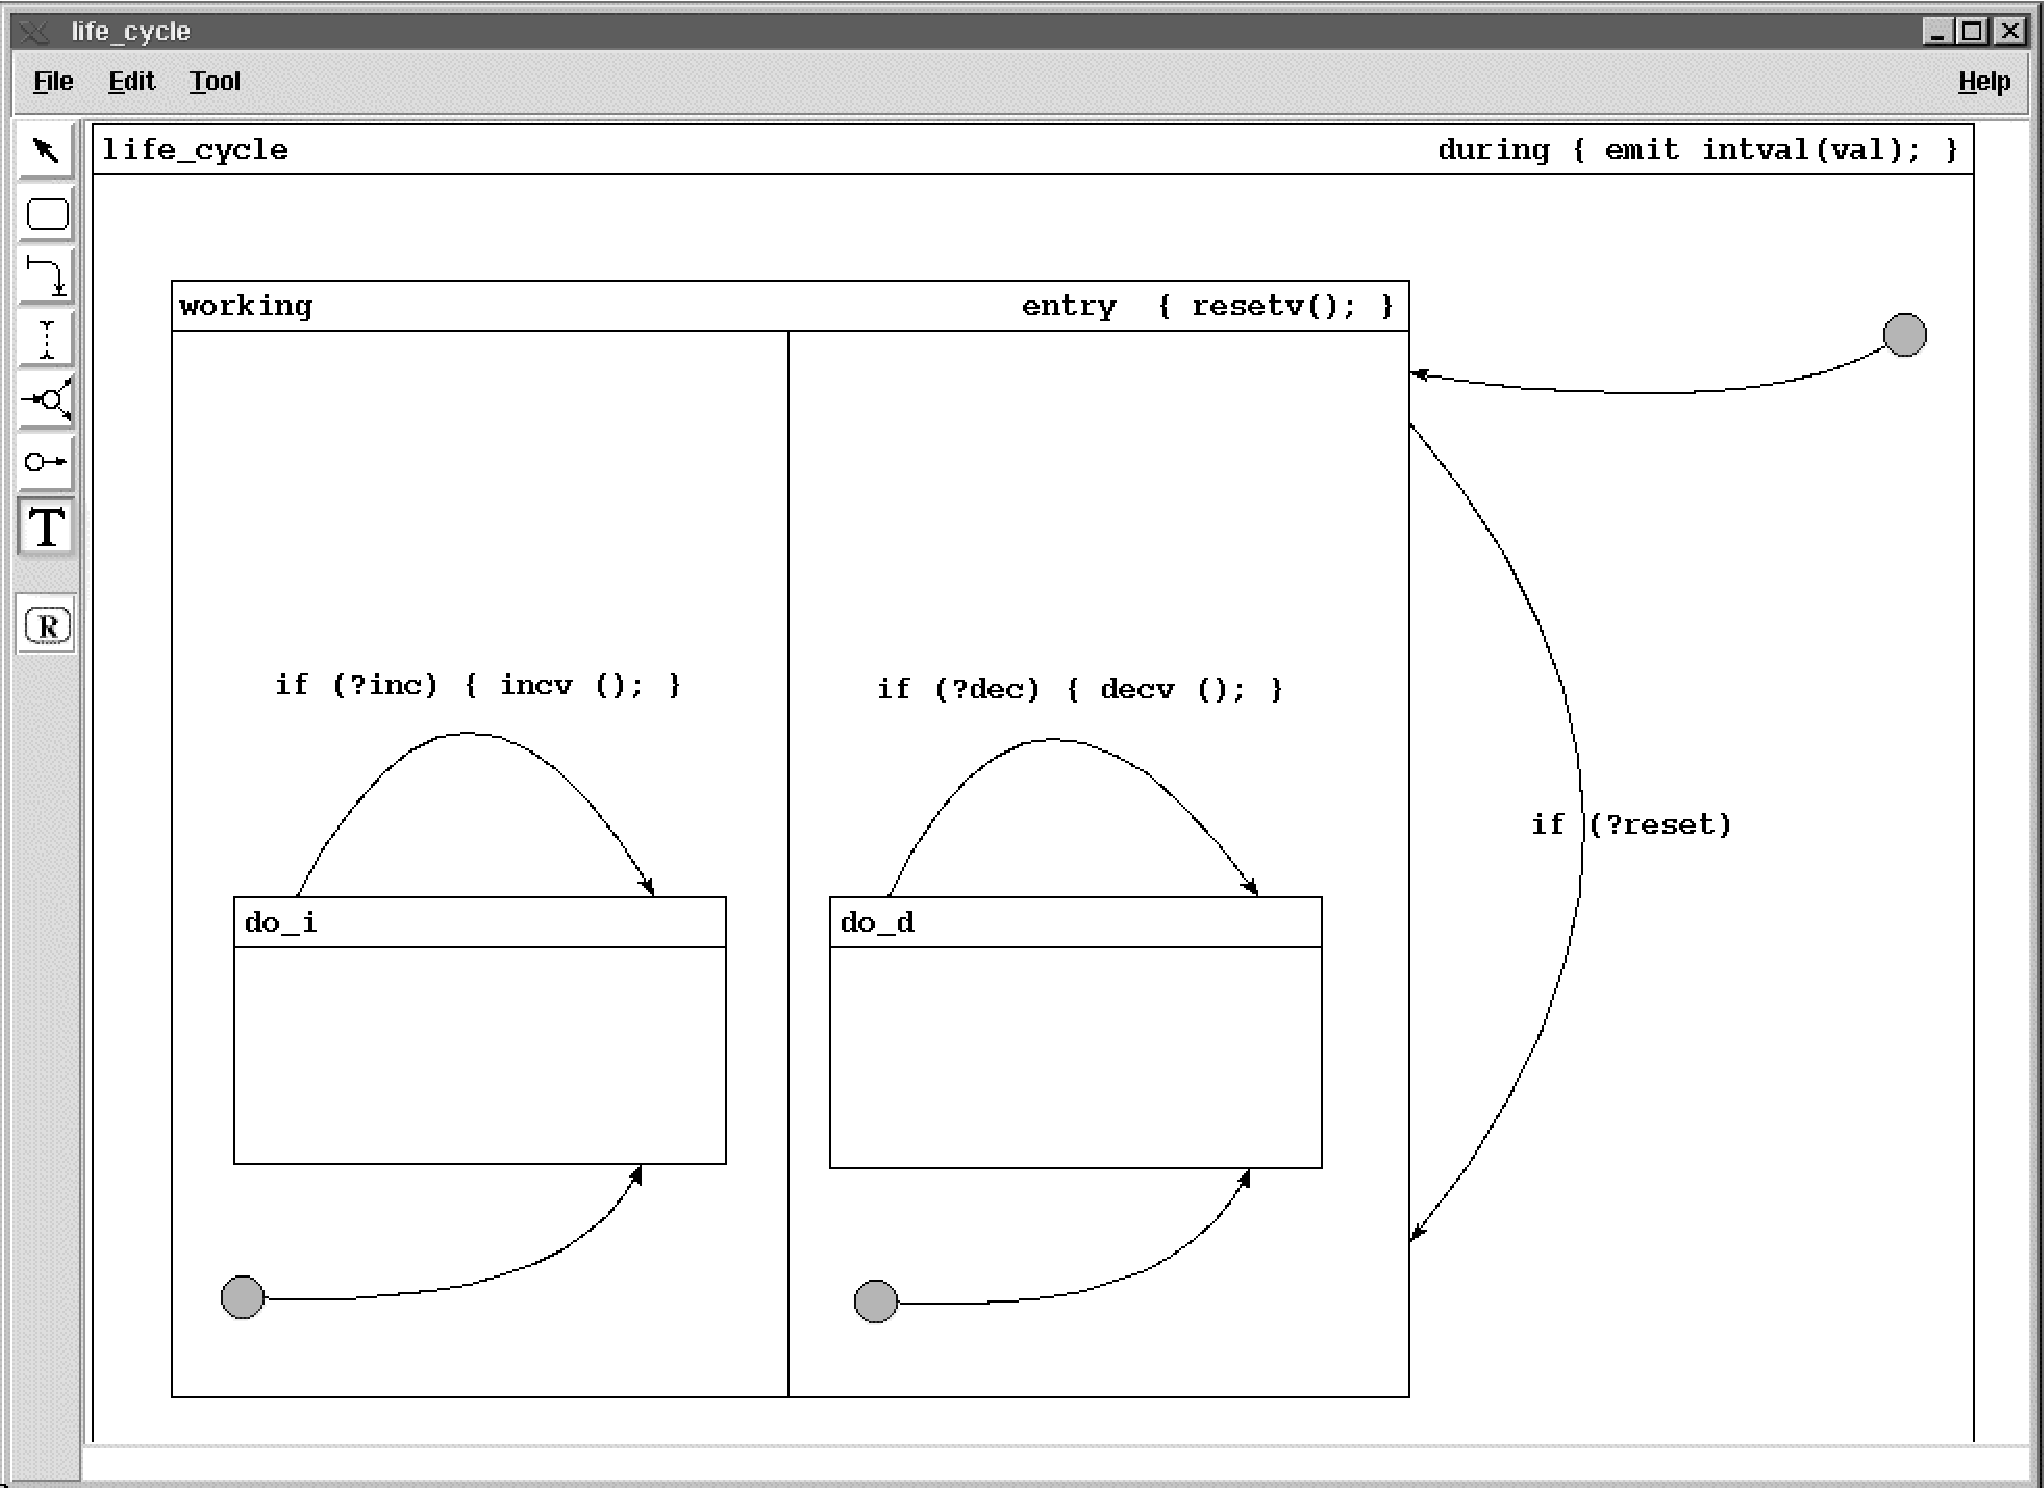
\includegraphics[width=250pt]{../pdf/incdec}
\end{center}

{\em
\section{\it Approximating \statecharts\ Semantics.}\index{Statecharts!semantics}

Emittance of signals is always delayed in \statecharts. Hence delayed signals as introduced in Section~\ref{reactive-control} may be used to approximate the \statecharts\ semantics.

There has been a certain amount of discussion whether the statecharts interpretation is truely synchronous. Rather than to join the flame, we believe that both signals and delayed signals have their merits and their shortcomings. Delayed signals cut causality cycles but a ``reaction'' may take more than one instant. The delays caused by delayed signals may be difficult to compute. Consider, for example, the familiar four bit counter but replacing signals by delayed signals.
% 
\codeinput{delayed-four-bit-automaton}
% 
Let us assume that we are in the states \emph{\pp{up1}} and \emph{\pp{up2}}, and let \emph{\pp{incr}} be present.  Then \emph{\pp{carry}} is emitted for the next
instant, and the first subautomaton moves to the state \emph{\pp{down1}}.  In
the next instant, the signal \emph{\pp{carry}} is present, the state of the
second subautomaton is change to \emph{\pp{down2}}, and the signal \emph{\pp{reset}} is emitted for the next instant.  At the same instant \emph{\pp{incr}} may be present causing a move to state \\emph{pp{up1}}. Now in the next instant, the signal  \emph{\pp{reset}} is present, the signal  \emph{\pp{elapsed}} is emitted for  the next instant, and toplevel automaton moves to state \emph{\pp{off}}. 

Of course, the process does not behave like a counter. We like to stress that the behaviour is not so easy to trace if delayed signals are involved, the main disadvantage being that mistakes will only show at run time.
}

\section{Examples}

\subsection{The Stopwatch using Automaton}\label{stopwatch-automaon}

\paragraph{The simple stopwatch.}
We distinguish two states: the stopwatch being running, and the stopwatch being stopped. The stopwatch toggles between the states if the button \pp{start\_stop} is pressed.
% 
\codeinput{simple-stopwatch-automaton}
%
One should note a distinction to the stopwatch as defined in Section \ref{stopwatch}. Since preemption is weak the elapsed time is emitted if the signal \pp{start\_stop} is present in state \pp{running}. It is a design choice whether this should be the case or not. For the latter, we must use strong preemption.


\paragraph{The general stopwatch}
Analysing the general stopwatch of Section \ref{stopwatch} we realise that there are two states corresponding to the simple stopwatch, a further toggle between the \pp{running} state, and a state for reset. These are used in the automaton below
% 
\codeinput{stopwatch-general-automaton}
%
One should note that -- quite unlike to the approach using the ``imperative'' sublanguage -- designing in terms of automata ask for finding states. It seems that in case of the general stopwatch this results in a much clearer design. The transitions between the states are obvious. however, the same remark applies as in case of the simple stopwatch above in that only weak preemption is used that results in a slightly different behaviour that that of the original stopwatch.



%\subsection{Another Lift Example}

%\subsection{A Telephone Answering Machine}
%




\chapter{Synchronous Data Flow}\label{data-flow}\index{data flow!synchronous}

Engineers use difference equations for modelling discrete-time systems.
Computer science speaks of synchronous data flow models.  The
synchronous programming language \lustre~\cite{lustre} is based on this
model as is \signal~\cite{signal}.  The data flow sub language of \se\
borrows much of the syntax and semantics of \lustre.

\section{Discrete Data Flow}\label{data-flow-informal}

\paragraph{Difference equations.}\index{difference equation}
A low pass filter removes the higher frequencies in a signal while passing the lower frequencies. A simple low pass filter is, for instance, specified by a \emph{difference equation} such as
% 
$$y[n] = 0.1 * x[n] + 0.9 * y[n-1]$$
% 
The index abstracts time since $n$ really stands for $t = nT$ where $T$ is an interval of time. Thus the equation is a shorthand for 
% 
$$y[nT] = 0.1 * x[nT] + 0.9 * y[(n-1)T]$$
% 
which should be read as ``at time $nT$ the value of of $y$ is equal to the sum of the the value of $x$ at time $nT$ multiplied by $0.1$ and of the value of $y$ at time $(n-1)T$ multiplied by $0.9$''.
:
Synchronous programming speaks of data flow equations rather than of
difference equations. There is a shift in semantics as well:
$x$ and $y$ are considered just as sequences of data with the value of $y$ being determined from that of $x$ in discrete steps by applying the difference equation. No timing is involved. In particular, no assumptions are made that the intervals in between two steps will be of equal length.

Flow equations abstract from indexes. The $n-1$ is replaced by an
explicit operator (\texttt{pre} in \se)
%
\begin{center}
\pp{y := 0.1 * x -> 0.1 * x + 0.9 * pre(y); }
\end{center}
%
The operator \pp{pre(x)} refers to the status of the signal \pp{x} at the 
\emph{previous} index.\footnote{Some may be
reminded of the Z-tranform.} The operator \pp{->} (\emph{arrow}) 
distinguishes between the  \emph{first} index -- the 
value being determined by the initialisation \pp{a0 * x} --, and 
\emph{later} indexes -- the value being determined by 
the expression \pp{a0 * x + a1 * pre(x) + b1 * pre(y)}.

\paragraph{Traces.} We will define the semantics of flow equations 
in terms of traces. Traces have been used in Chapter~\ref{classes} to
illustrate reactive behaviour. We will now start to use traces as a basis
for the semantics of reactive behaviour.

Let a \emph{trace}\index{trace} be a sequence of data (of the same type). At an instant,
a trace may be \emph{accessible}\index{accessible} or \emph{inaccessible}\index{inaccessible}. If it is accessible it has a value. For visualisation, we use a diagram of the form
\begin{center}
  \leavevmode
  \begin{tabular}[]{l@{\quad}||@{\quad} cccccccc}
    \hline\hline   
     \hbox{{\footnotesize \textit{i}}} &{\footnotesize \textit{0}}
     &{\footnotesize \textit{1}}&{\footnotesize \textit{2}}
     &{\footnotesize \textit{3}}&{\footnotesize \textit{4}}
     &{\footnotesize \textit{5}}&{\footnotesize \textit{6}}&\ldots
   \\  
    \hbox{$d$} &&$d_0$&$d_{1}$&&&$d_2$&&\ldots
   \\
   \hline\hline
  \end{tabular}
\end{center}
The trace $d$ is accessible at an instant if there is an entry $d_{n}$. An empty slot marks inaccessibility. The index $i$ indicates the instants.


Standard operators lift to the corresponding traces by defining the operations
element-wise at every instant, e.g.
\begin{center}
  \leavevmode
  \begin{tabular}[]{l@{\quad}||@{\quad} cccccccc}
    \hline\hline
     \hbox{{\footnotesize \textit{i}}} &{\footnotesize \textit{0}}
     &{\footnotesize \textit{1}}&{\footnotesize \textit{2}}
     &{\footnotesize \textit{3}}&{\footnotesize \textit{4}}
     &{\footnotesize \textit{5}}&{\footnotesize \textit{6}}&\ldots
   \\  
    \hbox{$d$} &&$d_0$&$d_1$&&&$d_2$&&\ldots
   \\
    \hbox{$d'$} &&$d'_0$&$d'_1$&&&$d'_2$&&\ldots
   \\
    \hbox{$d + d'$} 
    &&$d_0+d'_0$&$d_1+d'_1$&&&$d_2+d'_2$&&\ldots
   \\ 
   \hline\hline
  \end{tabular}
\end{center}
The definition requires that $d$, $d'$, and $d + d'$ are accessible at the same instant. 

Literals and variables determine traces. For instance, the literal \pp{3} determines a trace that has the value $3$ at every instant
\begin{center}
  \leavevmode
  \begin{tabular}[]{l@{\quad}||@{\quad} cccccccc}
    \hline\hline
     \hbox{{\footnotesize \textit{i}}} &{\footnotesize \textit{0}}
     &{\footnotesize \textit{1}}&{\footnotesize \textit{2}}
     &{\footnotesize \textit{3}}&{\footnotesize \textit{4}}
     &{\footnotesize \textit{5}}&{\footnotesize \textit{6}}&\ldots
   \\  
     \hbox{$d$} &$3$&$3$&$3$&$3$&$3$&$3$&$3$&\ldots
   \\
   \hline\hline
  \end{tabular}
\end{center}


\paragraph{Shifting time.}\index{time shift}\index{pre@\pp{pre}}
The operator $pre(d)$ shifts the trace $d$ in that it pointwise refers
to the \emph{previous} element 
\begin{center}
  \leavevmode
  \begin{tabular}[]{l@{}||@{\quad} cccccccc}
    \hline\hline
     \hbox{{\footnotesize \textit{i}}} &{\footnotesize \textit{0}}
     &{\footnotesize \textit{1}}&{\footnotesize \textit{2}}
     &{\footnotesize \textit{3}}&{\footnotesize \textit{4}}
     &{\footnotesize \textit{5}}&{\footnotesize \textit{6}}&\ldots
   \\  

    \hbox{$d$ \quad} &&$d_0$&$d_1$&&&$d_2$&&\ldots
   \\
    \hbox{\texttt{pre($d$)} \quad}  
    &&$\delta$&$d_0$&&&$d_1$&&\ldots
   \\
   \hline\hline
  \end{tabular}
\end{center}
The first element is a default value since there is no previous element. $\delta$ is a (type dependent, e.g. $0$ for integers, $false$ 
for booleans) default value. The trace \pp{pre($d$)} is accessible if and only if $d$ is accessible.

\paragraph{Initialising a trace.}\index{arrow (\pp{->})} The arrow operator distinguishes between the very first element of a trace, and all later elements.  
\begin{center}
  \leavevmode
  \begin{tabular}[]{l@{\quad}||@{\quad} cccccccc}
    \hline\hline
     \hbox{{\footnotesize \textit{i}}} &{\footnotesize \textit{0}}
     &{\footnotesize \textit{1}}&{\footnotesize \textit{2}}
     &{\footnotesize \textit{3}}&{\footnotesize \textit{4}}
     &{\footnotesize \textit{5}}&{\footnotesize \textit{6}}&\ldots
   \\  
    \hbox{$d$ \quad} &&$d_0$&$d_1$&&&$d_2$&&\ldots
   \\
    \hbox{$d'$} &&$d'_0$&$d'_1$&&&$d'_2$&&\ldots
   \\
   \hbox{\texttt{$d$ -> $d'$} } &&$d_0$&$d'_1$&&&$d'_2$&&\ldots
   \\
   \hline\hline
  \end{tabular}
\end{center}
The first element of the trace \texttt{$d$ -> $d'$} is the first element $d_{0}$ of the trace $d$ while the other elements are those of the trace $d'$. Note again that all the traces should be accessible at the same 
instants.

\paragraph{Flow equations.}\index{flow!equation}
The traces corresponding to a flow equation are inductively defined 
folllowing the structure of flow expressions. Here are two examples. The 
first example is an incrementing counter defined by the data flow 
equation
%
$$\pp{count := 0 -> pre(count) + 1;}$$
%
Here \texttt{count} is a signal of type \texttt{int}. At an instant,
the signal may be constrained by the flow equation, i.e. its value
is updated to be equal to the value of the expression on the right hand side. 
Hence the following behaviour is enforced.
\begin{center}
  \leavevmode
  \begin{tabular}[]{l@{\quad}||@{\quad}ccccccccccc}
    \hline\hline   
     \hbox{{\footnotesize \textit{i}}} &{\footnotesize \textit{0}}
     &{\footnotesize \textit{1}}&{\footnotesize \textit{2}}
     &{\footnotesize \textit{3}}&{\footnotesize \textit{4}}
     &{\footnotesize \textit{5}}&{\footnotesize \textit{6}}&\ldots
   \\  
    \hbox{$count$} 
    &$\mathbf{0}$&$\mathbf{1}$&$\textbf{2}$&$\mathbf{3}$&$\mathbf{4}$&
    $\mathbf{5}$&$\mathbf{6}$&$\mathbf{7}$&\ldots
   \\
    \hbox{$pre(count)$} &$\mathbf{0}$&$\mathit{0}$&$\mathit{1}$&$\mathit{2}$&
    $\mathit{3}$&$\mathit{4}$&$\mathit{5}$&$\mathit{6}$&\ldots
   \\    
    \hbox{$pre(count) + 1$} 
    &$\mathit{1}$&$\mathit{1}$&$\mathit{2}$&$\mathit{3}$&
    $\mathit{4}$&$\mathit{5}$&$\mathit{6}$&$\mathit{7}$&\ldots
   \\
    \hbox{$0\ \pp{->}\ pre(count) + 1$} 
	 &$\mathit{0}$&$\mathit{1}$&$\mathit{2}$&$\mathit{3}$&
	 $\mathit{4}$&$\mathit{5}$&$\mathit{6}$&$\mathit{7}$&\ldots
   \\
     \hline\hline
  \end{tabular}
\end{center} 
%For $n = 0$, we have $x(0) = 0$ due to the arrow operator. By 
%induction we can then prove that $x(n) = n$ for all $n$.
Let us assume that the signal \texttt{count} is updated at every instant
(implying that the signal is accessible). Let us say that a signal is present
if it is constrained by a flow equation. Presence is indicated by the bold typeface. 

In case of the (Boolean) flow expression 
%
$$\pp{raising\_edge : = false -> x \&\& !pre(x)}$$
%
 we may have the following table ($f$ stands for \emph{false}, and 
$t$ for \emph{true}) 
\begin{center}
  \leavevmode
  \begin{tabular}[]{l@{}||@{\quad}ccccccccccc}
    \hline\hline
     \hbox{{\footnotesize \textit{i}}} &{\footnotesize \textit{0}}
     &{\footnotesize \textit{1}}&{\footnotesize \textit{2}}
     &{\footnotesize \textit{3}}&{\footnotesize \textit{4}}
     &{\footnotesize \textit{5}}&{\footnotesize \textit{6}}
     &{\footnotesize \textit{7}}&\ldots
   \\  
    \hbox{$x$}
    &$f$&$t$&$t$&$f$&$f$&$t$&$f$&$t$&\ldots
   \\ 
    \hbox{$pre(x)$} &$f$&$f$&$t$&$t$&$f$&$f$&$t$&$f$&\ldots
   \\    
    \hbox{$! pre(x)$} &$t$&$t$&$f$&$f$&$t$&$t$&$f$&$t$&\ldots
   \\
    \hbox{$x\ {\tiny \&\&}\ !\ pre(x)$} &$f$&$t$&$f$&$f$&$f$&$t$&$f$&$t$&\ldots
   \\
    \hbox{$false\ \pp{->}\ x\ {\tiny \&\&}\ !pre(x)$\quad}
		&$f$&$t$&$f$&$f$&$f$&$t$&$f$&$t$&\ldots
   \\
    \hbox{$raising\_edge$\quad}
		&$\mathbf{f}$&$\mathbf{t}$&$\mathbf{f}$&$\mathbf{f}$&
		$\mathbf{f}$&$\mathbf{t}$&$\mathbf{f}$&$\mathbf{t}$&\ldots
	\\   \hline\hline
  \end{tabular}
\end{center}
The expression detects what hardware people call a \emph{raising 
edge}, i.e. the instants when the signal \texttt{x} changes from \emph{false} 
to \emph{true}.

\paragraph{A uniform view of updating.}
We note that signals my be updated
\begin{itemize}
\item either by emitting it as explained in the previous chapter,

\item or by constraining it by a flow equation.
\end{itemize}
Though conceptually quite different, both methods of updating behave equivalently in that
\begin{itemize}
\item if a signal is updated, either by emitting or constraining, it is present with a new value (if valued), and in that

\item multiple updating, either by emitting or constraining, of a signal at 
the same instant is a time race causing an error message.
\end{itemize}
However,
\begin{itemize}
\item \emph{flow equations support a richer language} including the time 
shift operators (and sampling operations, as we will learn in Section~\ref{multi-clock}).
\end{itemize}
%


\section{Embedding Data Flow to Control}\label{embedding}

\paragraph{Flow contexts.}\index{flow!context|textbf}
Flow equations are only allowed to occur in a particular context of the form
$$\texttt{\{| \ldots\  |\}}$$
We speak of a \emph{flow context}. Its body consists of a sequence of
flow equations (and of local signal declarations, see below).

Restricting the occurrence of flow equations to a particular context has the advantage that ambiguity of typing can be avoided: we stipulate that 
\emph{only flows can occur within a flow context}.
 Then an expression such as \pp{3 + 5} 
then has different interpretations within or outside of a flow context.
\begin{itemize}
\item Outside of a flow context, the terms \pp{3}, \pp{5}, and \pp{3 + 5} denote integers, and the addition operation operates on integers.

\item Within a flow context, the terms \pp{3}, \pp{5}, and \pp{3 + 5} are integer flows, and the addition operator operates on integer flows.

\item \emph{Note the operators \pp{pre} and \pp{->} can only be used within a flow context.}
\end{itemize}

The order of presentation of flow equations within a flow context is 
irrelevant for evaluation. The flow equation are evaluated by an
order imposed by the equations: if a signal is used 
within a flow expression on some right its value must be computed 
before the expression can be evaluated (\emph{write-before-read}), except
if the signal is ``guarded'' by a \texttt{pre}. In that case, a value is used
that has been computed at some previous instant. Here are some schematic 
examples for illustration:
\begin{itemize}
\item The two flow contexts
%
\BEP
   \{|  x := 0 -> pre(y);
       y := 2 * x;
   |\}    
\EEP
%
and
%
\BEP
   \{|  y := 2 * x;
       x := 0 -> pre(y);
   |\} 
\EEP   
%
behave equivalently; the flow equation for signal \texttt{x} must be
evaluated before that for signal \texttt{y} since it is used on the right
hand side of the flow equation for signal \texttt{y}.

\item The flow equations 
%
\BEP
   \{|  x := 0 -> y;
       y := 2 * x;
   |\}    
\EEP
%
will raise a causality error\index{causality!cycle}. We have a cyclic dependency since the flow
equation for \texttt{x} uses the value of \texttt{y} of the same instant,
and vice versa. Note that guarding \texttt{y} with a \texttt{pre} in the
equations above breaks the cycle, since the value of \texttt{y} of a previous
instant is used.

\end{itemize}
The notation $\texttt{\{| \ldots\  |\}}$ is meant to indicate that the 
order of presentation of flow equations is not relevant. 
Of course, for each signal, there should be at most one flow equation in any
flow context.

\paragraph{The watchdog example.} We rephrase the ``watchdog'' example of \cite{halbwachs}. The watchdog is a device to manage deadlines. There are three Boolean signals \pp{set}, \pp{reset}, and \pp{deadline}. The signals
\pp{set} and \pp{reset} switch the watchdog ``on'' and ``off''. If the watchdog is ``on'', and if the signal \pp{deadline} is true, the signal \pp{alarm} is true.
%
\codefragment{watchdog-body}
%
The formulation uses the conditional.
A hardware designer might prefer to use Boolean operators only, which 
yields a (disputably) more elegant solution.
%
\codefragment{watchdog-bool}
%
Note that ``setting the watchdog'' has precedence over resetting. The
precedence is reversed by using
%
\codefragment{watchdog-bool-2}
%

\paragraph{Modes.}\index{mode} 
It is somewhat inherent that the  evaluation of flow equations 
should be sustained for some time. 
This is achieved by using (a variant of) the \pp{sustain}\index{sustain@\pp{sustain}} statement
%
\BEP
    sustain \{|
       \ldots
    |\};
\EEP
%
Once started, the \pp{sustain} process never terminates; flow 
constraints are applied forever. We shall speak of a \emph{mode} (of 
operation). The idea is that modes persist, usually for a long interval,
but modes may be changed if necessary, for instance from a start-up mode
to a working mode, or from a working mode to an error mode or maintenance mode, 
and vice versa.

Being a process like any other, the sustain statement may be preempted and (re-) started as in
%
\codefragment{counting-up}
%
A trace of this fragment may look like as follows
\begin{center}
  \leavevmode
  \begin{tabular}[]{l@{\quad}||@{\quad}ccccccccccccc}
    \hline\hline
     \hbox{{\footnotesize \textit{i}}} &{\footnotesize \textit{0}}
     &{\footnotesize \textit{1}}&{\footnotesize \textit{2}}
     &{\footnotesize \textit{3}}&{\footnotesize \textit{4}}
     &{\footnotesize \textit{5}}&{\footnotesize \textit{6}}
     &{\footnotesize \textit{7}}&{\footnotesize \textit{8}}
     &{\footnotesize \textit{9}}&\ldots
   \\      
   \hbox{$start$} &.&.&.&*&.&.&.&.&.&.&\ldots
   \\
    \hbox{$stop$} &.&.&.&.&.&.&*&.&.&.&\ldots
   \\     
   \hbox{$count$}&$\mathit{0}$&$\mathit{0}$&$\mathit{0}$&
   $\mathbf{1}$&$\mathbf{2}$&$\mathbf{3}$&
   $\mathbf{4}$&$\mathbf{5}$&$\mathit{4}$&$\mathit{4}$&\ldots
%   \\ 
%    \hbox{$pre(count)$} &.&.&.&$0$&$0$&$1$&$2$&$3$&$4$&.&\ldots
%   \\    
%    \hbox{$pre(count) + 1$} &.&.&.&$1$&$1$&$2$&$3$&$4$&$5$&.&\ldots
%   \\    
%    \hbox{$0\ \texttt{->}\ pre(count) + 1$}
%           &.&.&.&$0$&$1$&$2$&$3$&$4$&$5$&.&\ldots
   \\
  
  \hline\hline
  \end{tabular}
\end{center}
If the signal \texttt{start} is present, the flow context starts to be
sustained.  The flow equation is evaluated at every instant till
the signal \texttt{stop} is present. Whenever the flow equation is evaluated
the signal \texttt{count} is updated, hence increased. Then the sustained process terminates instantaneously when the signal \texttt{stop} is present. 

The presence of the pure signals \texttt{start} and
\texttt{stop} is indicated by an asterisk. The signal \texttt{start} is present at the 4th instant,
and the flow context is active from the 4th to the 8th instant.  

\paragraph{\textit{Mode automata.}}\label{mode-automata}\index{mode automaton} 
{\em If we combine state machines with flow equations we may consider states as corresponding to modes. This is the idea of \emph{mode automata} as 
presented in ~\cite{Maranchini}. The following example has two moses/states, counting upward and counting downward.
% 
\codeinput{up-and-down-counter-automaton}
%

The construction is somewhat clumsy in that we have to use the 
\pp{next} to avoid multiple constraints: since preemption is weak, 
the program may count upward, change state from \pp{\em up} to 
\pp{\em down}, and count downward at the same instant if the \pp{\em 
next} would not guard the \pp{\em sustain} clause. The idea, in fact, 
would be that the flow equations should be active only if a state is 
in control but not if control enters a state. Since this phenomenon 
is quite usual for mode automata, we allow to use flow equations in the 
\pp{\em during} clause of a state as in 
% 
\codeinput{up-and-down-counter-during}
%
Then the flow equations are active when being in a state,
 but not if entering a state. Thus multiple constraints are avoided.
}

\section{Flow Contexts and Locality}

\paragraph{Local Signals.}\index{signal!local}
Signals can be declared within a flow context as local variables. All the rules for local variables apply (cf. Section~\ref{local-signals}) except for
exception: the initialisation
may be dropped, i.e. the shorthand \texttt{Signal<$T$>} may be used instead of \texttt{Signal<$T$> = new Signal<$T$>();}.
The scope of the signal are all the subsequent statements within the flow context.

Of course, using local variables may substantially change behaviour. We
reconsider
%
\codefragment{counting-up-2}
%
If the \pp{sustain} statement is active, the signal \pp{count} is increased,
otherwise its value persists. A typical trace is
\begin{center}
  \leavevmode
  \begin{tabular}[]{l@{\quad}||@{\quad}ccccccccccccc}
    \hline\hline
     \hbox{{\footnotesize \textit{i}}} &{\footnotesize \textit{0}}
     &{\footnotesize \textit{1}}&{\footnotesize \textit{2}}
     &{\footnotesize \textit{3}}&{\footnotesize \textit{4}}
     &{\footnotesize \textit{5}}&{\footnotesize \textit{6}}
     &{\footnotesize \textit{7}}&{\footnotesize \textit{8}}
     &{\footnotesize \textit{9}}&\ldots
   \\      
    \hbox{$start$} &.&$*$&.&.&.&.&$*$&.&.&.&\ldots
   \\
    \hbox{$stop$} &.&.&.&$*$&.&.&.&$*$&.&.&\ldots
   \\     
   \hbox{$count$} &$\mathit{0}$&$\mathbf{1}$&$\mathbf{2}$&
   $\mathbf{3}$&$\mathit{3}$&$\mathit{3}$&
   $\mathbf{4}$&$\mathbf{5}$&$\mathit{5}$&$\mathit{5}$&\ldots
   \\ 
  \hline\hline
  \end{tabular}
\end{center}

If the signal \pp{count} is declared locally within the flow context, a new
incarnation of \pp{count} is generated when control enters the flow context.
%
\codefragment{counting-up-3}
%
The corresponding trace is 
\begin{center}
  \leavevmode
  \begin{tabular}[]{l@{\quad}||@{\quad}ccccccccccccc}
    \hline\hline
     \hbox{{\footnotesize \textit{i}}} &{\footnotesize \textit{0}}
     &{\footnotesize \textit{1}}&{\footnotesize \textit{2}}
     &{\footnotesize \textit{3}}&{\footnotesize \textit{4}}
     &{\footnotesize \textit{5}}&{\footnotesize \textit{6}}
     &{\footnotesize \textit{7}}&{\footnotesize \textit{8}}
     &{\footnotesize \textit{9}}&\ldots
   \\      
    \hbox{$start$} &.&$*$&.&.&.&.&$*$&.&.&.&\ldots
   \\
    \hbox{$stop$} &.&.&.&$*$&.&.&.&$*$&.&.&\ldots
   \\          
   \hbox{$count'$} &&$\mathbf{1}$&$\mathbf{2}$&$\mathbf{3}$&&&&&&&\ldots
   \\
   \hbox{$pre(count')$} &&$\mathit{0}$&$\mathit{1}$&$\mathit{2}$&&&&&&&\ldots
   \\   
   \hbox{$pre(count')+1$}   &&$\mathit{1}$&$\mathit{2}$&
   $\mathit{3}$&&&&&&&\ldots
   \\
   \hbox{$count''$} &&&&&&&$\mathbf{1}$&$\mathbf{2}$&&&\ldots
   \\  
   \hbox{$pre(count'')$} &&&&&&&$\mathit{0}$&$\mathit{1}$&&&\ldots
   \\  
   \hbox{$pre(count'')+1$} &&&&&&&$\mathit{1}$&$\mathit{2}$&&&\ldots
   \\
  \hline\hline
  \end{tabular}
\end{center}
Why is this so? Whenever
the flow context is started, a new incarnation of the signal \pp{count} is created. Since this incarnation is clearly not accessible at previous instants, \pp{pre(count)} is initialised with 
a default value (here $0$). 

\paragraph{The \texttt{pre} operator and locality.}\index{pre@\pp{pre}!locality of} The operator \pp{pre} may
be applied to an expression as in
%
\codeinput{counting-up-4}
%
We consider the expression \pp{pre(count + 1)} as a shorthand for
%
\codeinput{counting-up-5}
%
with the local signal name \pp{aux} being chosen appropriately. 
This implies that the value of the expression is set to a default value when
starting the flow context. The corresponding traces look like this
\begin{center}
  \leavevmode
  \begin{tabular}[]{l@{\quad}||@{\quad}ccccccccccccc}
    \hline\hline
     \hbox{{\footnotesize \textit{i}}} &{\footnotesize \textit{0}}
     &{\footnotesize \textit{1}}&{\footnotesize \textit{2}}
     &{\footnotesize \textit{3}}&{\footnotesize \textit{4}}
     &{\footnotesize \textit{5}}&{\footnotesize \textit{6}}
     &{\footnotesize \textit{7}}&{\footnotesize \textit{8}}
     &{\footnotesize \textit{9}}&\ldots
   \\      
    \hbox{$start$} &.&$*$&.&.&.&.&$*$&.&.&.&\ldots
   \\
    \hbox{$stop$} &.&.&.&$*$&.&.&.&$*$&.&.&\ldots
   \\          
   \hbox{$count$} &$\mathit{0}$&$\mathbf{0}$&$\mathbf{1}$&$\mathbf{2}$
   &$\mathit{2}$&$\mathit{2}$&$\mathbf{0}$&$\mathbf{1}$&
   $\mathit{1}$&$\mathit{1}$&\ldots
   \\
   \hbox{$count + 1$} &&$\mathit{1}$&$\mathit{2}$&$\mathit{3}$&
   &&$\mathit{1}$&$\mathit{2}$&&&\ldots
   \\   
   \hbox{$pre(count + 1)$} &&$\mathit{0}$&$\mathit{1}$&
   $\mathit{2}$&&&$\mathit{0}$&$\mathit{1}$&&&\ldots
   \\     \hline\hline
  \end{tabular}
\end{center}
The result may be \emph{surprising}. The general idea is that expressions within a flow context are accessible only if the flow context is active. Otherwise the expressions -- hence the result of is evaluation -- is inaccessible.

Since this may be confusing we issue a general warning:
\begin{itemize}
\item \emph{\textbf{All usages of the operator \emph{\pp{pre}} should be properly guarded by an initialisation using the arrow operator.}}
\end{itemize}


\paragraph{The arrow operator and locality.}\index{arrow (\pp{->})!locality of}

Initialisation by an arrow operator takes place \emph{whenever a flow context is started}. Consider
%
\codeinput{counting-up-6} with the signal \pp{count} being globally defined.
Whenever \pp{start} is present the flow context is started, and the signal count is initialised to $0$.
\begin{center}
  \leavevmode
  \begin{tabular}[]{l@{\quad}||@{\quad}ccccccccccccc}
    \hline\hline
     \hbox{{\footnotesize \textit{i}}} &{\footnotesize \textit{0}}
     &{\footnotesize \textit{1}}&{\footnotesize \textit{2}}
     &{\footnotesize \textit{3}}&{\footnotesize \textit{4}}
     &{\footnotesize \textit{5}}&{\footnotesize \textit{6}}
     &{\footnotesize \textit{7}}&{\footnotesize \textit{8}}
     &{\footnotesize \textit{9}}&\ldots
   \\      
    \hbox{$start$} &.&$*$&.&.&.&.&$*$&.&.&.&\ldots
   \\
    \hbox{$stop$} &.&.&.&$*$&.&.&.&$*$&.&.&\ldots
   \\          
   \hbox{$count$} &$\mathit{0}$&$\mathbf{0}$&$\mathbf{1}$&$\mathbf{2}$
   &$\mathit{2}$&$\mathit{2}$&$\mathbf{0}$&$\mathbf{1}$&
   $\mathit{1}$&$\mathit{1}$&\ldots
   \\     \hline\hline
  \end{tabular}
\end{center}
Remember that without initialisation the counter is increased steadily 
whenever the flow context is active.

\noindent\emph{Remark.} One may be seduced by as expression such as
%
\BEP
  x := 0 -> (1 -> pre(x) + 1 )
\EEP
%
to believe that the value of \pp{x} is $0$ at the first instant when starting a flow context, and $1$ at the second. However, the definition says that,
whatever the trace on the right hand side of \pp{0 -> \ldots} is, the value
is $0$ at the first instant. Hence the flow equation above behaves equivalently to
%
\BEP
  x := 0 -> pre(x) + 1
\EEP
%

\paragraph{\textit{Hybrid systems.}}\index{system!hybrid}\label{hybrid-system}
\emph{We use ``localised'' versions of the pre and the arrow operator to support
the specification of hybrid systems. Hybrid systems are characterized by the interaction of continuous parts, governed by differential or difference equations (difference equations only in our context), and by discrete parts, described by finite state machines, if-then-else rules, propositional and temporal logic. Hybrid systems switch between many operating modes where each mode is governed by its own characteristic dynamical laws. Mode transitions are triggered by variables crossing specific thresholds (state events), by the elapse of certain time periods (time events), or by external inputs (input events). Further it is usually required that each mode starts operating with defined initial conditions specified by a reset relation.
}

\emph{In \se, all ``continuous'' modes are encapsulated by flow context, while all
the other language constructs specify the discrete parts resp. the transitions. Now having local initialisation by the arrow operators provides
the means to specify a reset relation. The initial condition can depend 
on the status of (globally declared) signals at a previous instant that is accessed by using the operator \pp{pre}. This is the sort of rationale for
our ``localised'' interpretation of the operators \pp{->} and \pp{pre}.}\footnote{Note that this generalises the use of these operators in \lustre. \lustre\ programs have -- in our terminology -- only one mode. Hence initialisation by the arrow operator can take place only in the very first instant, as well as the operator \pp{pre} has a default value only in the first instant (forgetting about 
, see Section~\ref{multi-clock}).}


\emph{To give a simple example of a typical presentation of a hybrid systems we consider a bouncing ball with the following properties:}
\begin{itemize}
\item \emph{Motion is characterised by \emph{height} ($x_{1}$) and \emph{vertical} velocity ($x_{2}$)},
\item \emph{Continuous changes between bounces.}
\item \emph{Discrete change at bounce time.}
\item \emph{Dynamics summarised by}
\begin{itemize}
\item \emph{one \emph{mode} $q$ with a continuous behaviour specified by the equations}
\begin{eqnarray*}
\dot{x_{1}} & = & x_{2}\\
\dot{x_{2}} & = & -g
\end{eqnarray*}
 
\item \emph{one \emph{transition} from $q$ to $q$ guarded by the condition $h \leq 0$,
}\item \emph{a reset relation that keeps the height but reverses the direction of velocity and decreases it by a factor in that $x_{2}$ is set to 
$-cx_{2}$.} 
\end{itemize}
\end{itemize}

\emph{The behaviour is graphically specified by}
\begin{center}
	{\tt\small
       \thinlines
       \setlength{\unitlength}{0.9pt}
       \begin{picture}(140,100)
           \put(5,70){$x_{1} \leq 0$}
           \put(90,70){$x_{2} := -cx_{2}$}
           \put(65,76){\circle{50}}
           \put(79,59){\thicklines\vector(-2,-1){7}}
          \put(30,0){\Ovalbox{\begin{Beqnarray*}
                                      \\\ \dot{x_{1}} & = & x_{2}\
                                      \\\dot{x_{2}} & = & -g\\
                                 \end{Beqnarray*}}}       
       \end{picture}
     }
\end{center}
\emph{If we try to translate this to a program, the obvious is to 
replace an differential equation $\dot{x} = e$ is replaced by an integral 
$x = x_{0} +\int edx$, and to compute the integral using difference
equations such as, for instance:}
\begin{itemize}
  \item \emph{(forward) Euler}
	\begin{eqnarray*}
		  x_{1}(n) & = & x_{1}(n-1) + x_{2}(n-1) \times dt \\
		  x_{2}(n) & = & \left\{
		                  \begin{array}{lll}
		                       -c*x_{2}(n-1) &- g*dt&\mbox{if $x_{1} \le 0$} \\
		                          x_{2}(n-1) &- g*dt&\mbox{otherwise}
		                    \end{array}
		               \right.
	\end{eqnarray*}
  \item \emph{or backward Euler}
	\begin{eqnarray*}
		  x_{1}(n) & = & x_{1}(n-1) + x_{2}(n) \times dt \\
		  x_{2}(n) & = & \left\{
		                  \begin{array}{lll}
		                       -c*x_{2}(n-1) &- g*dt&\mbox{if $x_{1} \le 0$} \\
		                          x_{2}(n-1) &- g*dt&\mbox{otherwise}
		                    \end{array}
		               \right.
	\end{eqnarray*}
\end{itemize}	
\emph{Another choice maybe Runge-Kutta. For the example, backward Euler works. A corresponding \se\ program is}
%
\codeinput{bouncing-ball}
%
\emph{Whenever the state \pp{move} is entered, the speed is reversed. Note that 
forward Euler would fail: whenever the direction switches, the speed
is negative before the switch, and positive after. For backward Euler, we
would compute \emph{\pp{x1 := pre(x1) + pre(x2) * dt}} after the switch, but with
\pp{pre(x2)} which is the negative value of speed before the switch. Hence,
the height would decrease rather than increase after the switch, actully be 
less than $0$ again, causing another switch. Hence the height toggles about
$0$ while the speed decreases, which does not quite reflect the physics. }

\paragraph{\textit{Warning}} \emph{If compared with simulation tools such as
 Matlab/Simulink or Scilab/Scicos one should note that in case of 
 ``zero-crossings'' resolution of computation cannot be improved for
 better results: the $dt$ provides the finest resolution.
One should keep here in mind that the language is build for hard real-time
control. Hence we cannot artificially ``stretch time'' as can
be achieved for offline simulators. 
}

\emph{Hence one should not use an exact value such as $0.0$ for changing direction
but rather some $\epsilon$ ball, meaning replacing $o.o$ by a small positive value.}

\section{Examples}

\subsection{Using Flows for the Stopwatch}\label{stopwatch-flow}

 
\paragraph{The simple stopwatch.} The following fragment rephrases the
simple stopwatch of Section~\ref{stopwatch} using flow equations
%
\codeinput{flow-simple-stopwatch}
%
The signal \pp{running} is toggled if the sensor \pp{start\_stop} is true.
The displayed time is increased if in the running state, reset to $0$ if
the sensor \pp{reset} is true, and otherwise kept unchanged. 

\paragraph{The general stopwatch.}
The general stopwatch permits to record intermediate times. As in Section~\ref{stopwatch}, we introduce a signal \pp{elapsed\_time} that behaves like the signal \pp{display\_time} of the simple stopwatch. For the general stopwatch the signal \pp{display\_time} remains constant if the stopwatch is in state ``frozen''.  The signal
\pp{reset} has two functionalities: (i) if the stopwatch is stopped but not frozen then the time is reset to $0$ (by the signal \pp{actual\_reset}, and (b) it toggles between the states ``frozen'' and ``not froozen''.
%
\codeinput{flow-simple-stopwatch-with-intermediate-time}
%

\paragraph{\textit{The general stopwatch as a hybrid system.}}
\emph{The logic of the general stopwatch is quite intriguing and needs careful analysis for a proper understanding. This is due to the fact that the effect of sporadic control features such as pushing the \emph{\pp{start\_stop}} button or 
the \emph{\pp{reset}} button are implemented using logic. Using hybrid systems provides a much clearer design
%
\codeinput{flow-hybrid-stopwatch}
%
In state \emph{\pp{running}} both the internal and the displayed times are increased. In state \emph{\pp{frozen}} only the internal time is increased. One realizes that the stopwatch can be reset to \emph{\pp{0sec}} only if the process is neither in state \emph{\pp{running}} nor in state \emph{\pp{frozen}}. Further if being stopped the \emph{\pp{start\_stop}} button has precedence over the \emph{\pp{reset}} button. In the pure flow version this is rather implicit in that for evaluating the flow equation for the internal time the \emph{\pp{actual\_reset}} condition is only checked if the system is not running.}

\subsection{The Train Example Reconsidered.}\label{train-flow}
We rephrase the single line train example \ref{train} using data 
flow. We replace all the input and output signals by Boolean signals.  
There are two additional Boolean signals \pp{change} and 
\pp{priority}. The signal \pp{change} computes any change 
situation, and signal \pp{priority} the priority of trains 
as the name suggests. The priority is computed only if a change of 
situation takes place in that a new train arrives or a train leaves 
the single track.
To compute the change and the priority there are three more auxiliary 
Boolean signals \pp{trainWaiting}, 
\pp{trainArriving}, and \pp{lineFreed}. The latter is true at the 
instant a train leaves the single line. The meaning of the other two 
are obvious. 
% 
\codefragment{train-data-flow-equations}
%
The overall behaviour should be easy to grasp considering the 
explanations
given in Section~\ref{train}. The pointings are set according to the 
priority, and the traffic lights are set to green when the obvious 
conditions hold.

\subsection{The LEGO Example using Flows}

We present a flow variant of the robot example in
Section~\ref{lego-example}.  The wheeled robot is able to move
forward and backward, and to turn left and right.  Two bumper sensors
on the left and right front end are used to detect obstacles.  The
task is to control the robot such that it travels around without
being caught, for instance, in some corner.

\codeinput{travel-flow}

The sensors are encoded by the sensors \pp{lsensor}
and \pp{rsensor}. The motor actuators are \pp{ldir}, \pp{rdir}, 
\pp{lspeed}, and \pp{rspeed}.

\section{Reusing Data Flow Equations}

\paragraph{Block diagrams.}\index{block diagram} Engineers often prefer a visual 
presentation for data flows, e.g.
\begin{center}
	{\tt\small
       \thinlines
       \setlength{\unitlength}{0.9pt}
       \begin{picture}(220,50)
           \put(5,15){x}

           \put(0,25){\vector(1,0){120}}

           \put(20,5){\vector(1,0){10}}

           \put(20,25){\line(0,-1){20}}
           \put(30,0){\framebox(30,10){\footnotesize pre}}       
           \put(60,5){\vector(1,0){20}}

           \put(80,0){\framebox(20,10){!}}       
           \put(100,5){\line(1,0){10}}
           \put(110,5){\line(0,1){10}}
           \put(110,15){\vector(1,0){10}}

           \put(120,10){\framebox(20,20){\&\&}}       
           \put(140,20){\vector(1,0){50}}

           \put(145,15){
               \begin{picture}(60,35)
                   \put(0,25){\framebox(40,10){\footnotesize false}}
                   \put(15,15){\line(0,1){10}}
                   \put(15,15){\vector(1,0){25}}
                   \put(40,0){\framebox(20,20){->}}
               \end{picture}
           }
       \put(210,25){\vector(1,0){30}}

       \put(227,15){y}

       \end{picture}
     }
 \end{center}
The boxes represent operators (with constants being an operator of 
arity 0),  and arrows represent flows of data between these. The 
behaviour corresponds to that of the flow equation for finding a
raising edge
%
\BEP
y := false.. -> x \&\& ! pre(x);
\EEP
% 
Typically such block diagrams are abstracted by boxing in the diagram as in    
\begin{center}
 {\tt\small
   \thinlines
   \setlength{\unitlength}{0.8pt}
   \begin{picture}(120,25)
       \put(10,14){$x$}
       \put(90,14){$y$}
       \put(0,10){\vector(1,0){30}}
       \put(80,10){\vector(1,0){30}}          
       \put(30,0){\framebox(50,20){edge\_up}} 
             \end{picture}
 }
\end{center}
The new box may be used in other diagrams as a shorthand as in 
the following fragment of the train example in Section~\ref{train}
\begin{center}
 {\tt\scriptsize
   \thinlines
   \setlength{\unitlength}{0.8pt}
   \begin{picture}(440,100)
       \put(405,48){change}
       \put(400,45){\vector(1,0){40}}
       \put(380,30){\framebox(20,30){||}} 
       \put(370,55){\vector(1,0){10}}
       \put(370,55){\line(0,1){20}}
       \put(360,75){\line(1,0){10}}
 	    \put(340,60){\framebox(20,25){\&\&}} 
       \put(320,65){\vector(1,0){20}}
       \put(260,85){trainArriving}
       \put(140,85){trainWaiting}
       \put(130,80){\vector(1,0){80}}
       \put(110,65){\framebox(20,30){||}} 
       \put(0,90){\vector(1,0){110}}
       \put(0,80){rightTrainWaiting}
       \put(0,70){\vector(1,0){110}}
       \put(0,60){leftTrainWaiting}
       \put(255,80){\vector(1,0){85}}
       \put(210,70){\framebox(45,20){edge\_up}} 
       \put(320,50){\line(0,1){15}}
       \put(0,50){\line(1,0){320}}
       \put(0,40){isLineFree}
       \put(70,5){\line(0,1){45}}
       \put(70,5){\vector(1,0){20}}
       \put(135,5){\vector(1,0){205}}          
       \put(140,8){lineFreed}
       \put(90,-5){\framebox(45,20){edge\_up}} 
       \put(170,25){\line(0,1){55}}
       \put(170,25){\vector(1,0){170}}
       \put(370,35){\vector(1,0){10}}
       \put(370,15){\line(0,1){20}}
       \put(360,15){\line(1,0){10}}
       \put(340,0){\framebox(20,30){\&\&}} 
   \end{picture}
 }
\end{center}

Block diagrams provide a natural abstraction mechanism for structuring and for reuse in the world of data flow corresponding to method calls in an object-oriented world.

\paragraph{A textual presentation.}  Looking for a textual representation of block diagrams, we observe that
\begin{itemize}
\item a block is specified in terms of
   \begin{itemize}
      \item ingoing and outgoing flows, and
      \item a body being a flow context and that 
    \end{itemize}

\item a block is embedded in a diagram by connecting  the flows inside and outside of the block. 
\end{itemize}

The mechanism we use resembles that of reactive methods, but the body
only consist of a flow context, e.g\index{edge\_up@\pp{edge\_up}}
%
\codefragment{edge-up}
%
We speak of \emph{nodes}\index{node|textbf} rather than of blocks, hence the keyword. For connection, sensors and signals are passed as parameters as in
%
\BEP
edge\_up(isLineFree,LineFreed)
\EEP
%
Calling the node within a flow context then ``glues'' the boxes.
\codefragment{data-flow-train-nodes}

When compiling, each node call\index{node!call} is expanded by replacing the parameters by the arguments and by adding its flow equations to the enclosing flow context.
In case of the train example the code to execute is
\codefragment{data-flow-train-nodes-expanded}

\paragraph{Relational abstraction.}\index{abstraction!relational}
The general scheme is to have boxes with $m$ ingoing flows and $n$ outgoing flows
\begin{center}
 {\tt\small
   \thinlines
   \setlength{\unitlength}{0.8pt}
   \begin{picture}(120,55)
       \put(10,44){$x_{1}$}
       \put(120,44){$y_{1}$}
       \put(0,40){\vector(1,0){30}}
       \put(110,40){\vector(1,0){30}} 
       \put(10,31){.}      
       \put(10,27){.}      
       \put(10,23){.}      
       \put(120,31){.}      
       \put(120,27){.}      
       \put(120,23){.}   
       \put(10,14){$x_{m}$}
       \put(120,14){$y_{n}$}
       \put(0,10){\vector(1,0){30}}
       \put(110,10){\vector(1,0){30}}          
       \put(30,0){\framebox(80,50){xxxx}} 
   \end{picture}
 }
\end{center}
The corresponding textual counterpart adds type information 
%
\BEP
node xxxx ( Sensor<$T_{1}$>$   x_{1}$, \ldots , Sensor<$T_{m}$>$   x_{m}$,
            Signal<$T_{m+1}$>$ y_{1}$, \ldots , Signal<$T_{m+n}$>$ y_{n}$ ) \{|

  ...
  
|\};
\EEP
%
The body is restricted to be a flow context.

A node specifies a relation for constraining flows, just as flow equations do. Hence a node may be only called within a flow context. If the flow context is active at an instant, the constraints of the flow equations apply as well as those that are specified by a node called.\footnote{Here, \se\ substantially differs from \lustre\ that uses functional abstraction.}

%We restrict the \emph{actual parameters of flow equations to be flow variables or flow signals only} for pragmatic reasons: if a parameter is ``outgoing'', i.e. it appears on the left side of a flow equation in the body of a flow method, then it should be constrained by the respective flow equation in that it the right hand side constrains the left hand side. This implicit direction of constraining flows would be violated if a flow expression such as, e.g. $3$, is an actual argument for an ``outgoing'' flow
%parameter. Though not strictly necessary, we apply the same convention for ``ingoing'' parameters. Though this may sometimes raise the need of adding auxiliary variables, the code tends to be more readable.

\paragraph{The stopwatch again.}
The stopwatch of Section~\ref{stopwatch-flow} is an example for using a flow method with multiple input and output flows. The simple stopwatch becomes the flow method
%
\codefragment{flow-stopwatch-method-simple-stopwatch}
%
This method is called within a flow context as follows
%
\codeinput{flow-stopwatch-general}
%

%\subsection{Functional Abstraction}\index{abstraction!functional}
%The example above might



\section{\textit{On Clocks}}\label{multi-clock}

{\em

\paragraph{\textit{Sampling signals.}}\index{sampling} 
Execution of a flow equations consumes real time. Hence one may sometimes 
want to avoid executing a data flow equation at every instant. Let, for 
example, the input $x$ of the filter equation 
$$y(n) = a_0 * x(n) + a_1 * x(n-1) - b_1 * y(n-1),$$
be given by a curve such as 
\begin{center}
 {\tt\scriptsize
   \thinlines
   \setlength{\unitlength}{1pt}
   \begin{picture}(205,60)
   \put(0,20){\line(1,0){205}}
   \put(5,30){\bezier{200}(0,20)(35,30)(55,-10)}
   \put(60,20){\bezier{200}(0,0)(15,-30)(30,0)}
   \put(90,20){\bezier{200}(0,0)(20,40)(70,20)}
   \put(160,20){\bezier{200}(0,20)(20,10)(40,20)}
   \put(5,20){\line(0,1){30}}   
   \put(10,20){\line(0,1){31}}   
   \put(15,20){\line(0,1){32}}   
   \put(20,20){\line(0,1){32}}   
   \put(25,20){\line(0,1){31}}   
   \put(30,20){\line(0,1){30}}   
   \put(35,20){\line(0,1){28}}   
   \put(40,20){\line(0,1){26}}   
   \put(45,20){\line(0,1){22}}   
   \put(50,20){\line(0,1){15}}   
   \put(55,20){\line(0,1){8}}
   \put(65,20){\line(0,-1){8}}   
   \put(70,20){\line(0,-1){13}} 
   \put(75,20){\line(0,-1){15}} 
   \put(80,20){\line(0,-1){13}} 
   \put(85,20){\line(0,-1){9}} 
   \put(95,20){\line(0,1){9}} 
   \put(100,20){\line(0,1){15}}
   \put(105,20){\line(0,1){19}} 
   \put(110,20){\line(0,1){22}}
   \put(115,20){\line(0,1){24}}
   \put(120,20){\line(0,1){25}}
   \put(125,20){\line(0,1){26}}
   \put(130,20){\line(0,1){26}}
   \put(135,20){\line(0,1){26}}
   \put(140,20){\line(0,1){25}}
   \put(145,20){\line(0,1){24}}
   \put(150,20){\line(0,1){23}}
   \put(155,20){\line(0,1){22}}
   \put(160,20){\line(0,1){20}}
   \put(165,20){\line(0,1){18}}
   \put(170,20){\line(0,1){17}}
   \put(175,20){\line(0,1){16}}
   \put(180,20){\line(0,1){15}}
   \put(185,20){\line(0,1){16}}
   \put(190,20){\line(0,1){17}}
   \put(195,20){\line(0,1){18}}
   \put(200,20){\line(0,1){20}}   
   \end{picture}
 }
\end{center}
For reasons of efficiency, one want to compute the filter equation only every other instant
\begin{center}
 {\tt\scriptsize
   \thinlines
   \setlength{\unitlength}{1pt}
   \begin{picture}(205,60)
   \put(0,20){\line(1,0){205}}
   \put(5,30){\bezier{200}(0,20)(35,30)(55,-10)}
   \put(60,20){\bezier{200}(0,0)(15,-30)(30,0)}
   \put(90,20){\bezier{200}(0,0)(20,40)(70,20)}
   \put(160,20){\bezier{200}(0,20)(20,10)(40,20)}
   \put(5,20){\line(0,1){30}}   
   \put(15,20){\line(0,1){32}}   
   \put(25,20){\line(0,1){31}}   
   \put(35,20){\line(0,1){28}}   
   \put(45,20){\line(0,1){22}}   
   \put(55,20){\line(0,1){8}}
   \put(65,20){\line(0,-1){8}}   
   \put(75,20){\line(0,-1){15}} 
   \put(85,20){\line(0,-1){9}} 
   \put(95,20){\line(0,1){9}} 
   \put(105,20){\line(0,1){19}} 
   \put(115,20){\line(0,1){24}}
   \put(125,20){\line(0,1){26}}
   \put(135,20){\line(0,1){26}}
   \put(145,20){\line(0,1){24}}
   \put(155,20){\line(0,1){22}}
   \put(165,20){\line(0,1){18}}
   \put(175,20){\line(0,1){16}}
   \put(185,20){\line(0,1){16}}
   \put(195,20){\line(0,1){18}}
   \end{picture}
 }
\end{center}
The filter equation turns into
$$y(2*n) = a_0 * x(2*n) + a_1 * x(2*(n-1)) - b_1 * y(2*(n-1))$$
The formalisation gets messy though if we want to sample the curve
only if its amplitude is below a certain threshold as in
\begin{center}
 {\tt\scriptsize
   \thinlines
   \setlength{\unitlength}{1pt}
   \begin{picture}(205,60)
   \put(0,20){\line(1,0){205}}
   \put(5,30){\bezier{200}(0,20)(35,30)(55,-10)}
   \put(60,20){\bezier{200}(0,0)(15,-30)(30,0)}
   \put(90,20){\bezier{200}(0,0)(20,40)(70,20)}
   \put(160,20){\bezier{200}(0,20)(20,10)(40,20)}
   \dashline{5}(0,42)(200,42)
   \put(45,20){\line(0,1){22}}   
   \put(50,20){\line(0,1){15}}   
   \put(55,20){\line(0,1){8}}
   \put(65,20){\line(0,-1){8}}   
   \put(70,20){\line(0,-1){13}} 
   \put(75,20){\line(0,-1){15}} 
   \put(80,20){\line(0,-1){13}} 
   \put(85,20){\line(0,-1){9}} 
   \put(95,20){\line(0,1){9}} 
   \put(100,20){\line(0,1){15}}
   \put(105,20){\line(0,1){19}} 
   \put(110,20){\line(0,1){22}}
   \put(155,20){\line(0,1){22}}
   \put(160,20){\line(0,1){20}}
   \put(165,20){\line(0,1){18}}
   \put(170,20){\line(0,1){17}}
   \put(175,20){\line(0,1){16}}
   \put(180,20){\line(0,1){15}}
   \put(185,20){\line(0,1){16}}
   \put(190,20){\line(0,1){17}}
   \put(195,20){\line(0,1){18}}
   \put(200,20){\line(0,1){20}}   
   \end{picture}
 }
\end{center}

\se\ provides a very simple mechanism to deal with down-sampling. The 
operator 
\begin{center}
\emph{\pp{$E$ when $C$}}
\end{center}
states that the expression $E$ is evaluated only if the condition $C$ 
becomes true. 

Hence the flow equations
\begin{quote}
\emph{\pp{y := (a0 * x + a1 * pre(x) + 
b1 * pre(y)) when c;\\
c := false -> !pre(c);}}
\end{quote}
express precisely that the filter equation is evaluated only every other
instant. Restricting sampling by a threshold is neatly expressed by 
\begin{quote}
\emph{\pp{y := (a0 * x + a1 * pre(x) + 
b1 * pre(y)) when (x < up);}}
\end{quote}
and both may be combined to
\begin{quote}
\emph{\pp{y := (a0 * x + a1 * pre(x) + 
b1 * pre(y)) when (c \& x < up);\\
c := false -> !pre(c);}}
\end{quote}
as visualised by
\begin{center}
 {\tt\scriptsize
   \thinlines
   \setlength{\unitlength}{1pt}
   \begin{picture}(205,60)
   \put(0,20){\line(1,0){205}}
   \put(5,30){\bezier{200}(0,20)(35,30)(55,-10)}
   \put(60,20){\bezier{200}(0,0)(15,-30)(30,0)}
   \put(90,20){\bezier{200}(0,0)(20,40)(70,20)}
   \put(160,20){\bezier{200}(0,20)(20,10)(40,20)}
   \dashline{5}(0,42)(200,42)
   \put(45,20){\line(0,1){22}}   
   \put(55,20){\line(0,1){8}}
   \put(65,20){\line(0,-1){8}}   
   \put(75,20){\line(0,-1){15}} 
   \put(85,20){\line(0,-1){9}} 
   \put(95,20){\line(0,1){9}} 
   \put(105,20){\line(0,1){19}} 
   \put(155,20){\line(0,1){22}}
   \put(165,20){\line(0,1){18}}
   \put(175,20){\line(0,1){16}}
   \put(185,20){\line(0,1){16}}
   \put(195,20){\line(0,1){18}}
   \end{picture}
 }
\end{center}

We used a bit of hand waving here. Precisely, the right hand side of the
equation is down-sampled only using the operator \emph{\pp{when}}, but not
the left hand side. If we reconsider the down-sampled filter equation
$$y(2*n) = a_0 * x(2*n) + a_1 * x(2*(n-1)) - b_1 * y(2*(n-1))$$
the down-sampling (multiplying by $2$) applies to both sides. We express
down-sampling of signals as an annotation to the signal type, e.g.
\begin{center}
\emph{\pp{Signal\{c \& x < up\}<double> y;}}
\end{center} 
We refer to the expression \emph{\emph{\pp{c \& x < up}}} as a \emph{clock}\index{clock}.
The idea is that a signal can only be updated by a flow constraint
at an instant if the clock condition evaluates to true at that instant.
Clearly, the signal and the expression on the right hand side of a flow
equation should ``be on the same clock'' (this will be made precise further below).

\paragraph{\textit{Sampling operators.}} 
The operator \emph{\pp{when}} \emph{down-samples}\index{down-sampling}\index{when@\pp{when}} the trace $d$ at a \emph{frequency} specified by the Boolean ``clock'' flow $c$ as in, e.g.,
\begin{center}
  \leavevmode
  \begin{tabular}[]{l@{\quad}||@{\quad} ccccccccccc}
    \hline\hline  
     \hbox{{\footnotesize \textit{i}}} &{\footnotesize \textit{0}}
     &{\footnotesize \textit{1}}&{\footnotesize \textit{2}}
     &{\footnotesize \textit{3}}&{\footnotesize \textit{4}}
     &{\footnotesize \textit{5}}&{\footnotesize \textit{6}}
     &{\footnotesize \textit{7}}&{\footnotesize \textit{8}}
     &{\footnotesize \textit{9}}&\ldots
   \\      
    \hbox{$d$} &&$d_0$&$d_{1}$&&&$d_2$&&$d_3$&$d_4$&&\ldots
   \\
    \hbox{$c$} &&$t$&$f$&&&$f$&&$t$&$f$&&\ldots
   \\
    \hbox{\pp{$d$\ when\ $c$}} &&$d_0$&&&&&&$d_3$&&&\ldots
   \\
      \hline\hline
  \end{tabular}
\end{center}
The flow $d\ \emph{\pp{when}}\ b$ is accessible at an instant if and only 
if the flow $b$ has the value $true$ at that instant.

We expect {\em up-sampling}\index{up-sampling}\index{current@\pp{current}} as a counter part to down-sampling. The 
operator \emph{\pp{current}} latches the value of a trace till the next sampling.
\begin{center}
  \leavevmode
  \begin{tabular}[]{l@{\quad}||@{\quad} ccccccccccc}
    \hline\hline  
     \hbox{{\footnotesize \textit{i}}} &{\footnotesize \textit{0}}
     &{\footnotesize \textit{1}}&{\footnotesize \textit{2}}
     &{\footnotesize \textit{3}}&{\footnotesize \textit{4}}
     &{\footnotesize \textit{5}}&{\footnotesize \textit{6}}
     &{\footnotesize \textit{7}}&{\footnotesize \textit{8}}
     &{\footnotesize \textit{9}}&\ldots
   \\      
    \hbox{$d$} &&$d_0$&$d_{1}$&&&$d_2$&&$d_3$&$d_4$&&\ldots
   \\
    \hbox{$c$} &&$t$&$f$&&&$f$&&$t$&$f$&&\ldots
   \\
    \hbox{\pp{$e = d$\ when\ $c$}} &&$d_0$&&&&&&$d_3$&&&\ldots
   \\
    \hbox{\pp{current($e$)}} &&$d_0$&$d_0$&&&$d_0$&&$d_3$&$d_3$&&\ldots
   \\
      \hline\hline
  \end{tabular}
\end{center}

Up-sampling should generate a trace that is ``as fast'' as the trace originally down-sampled meaning that \pp{current($d'$)} is accessible 
if and only if $d$ (resp. $c$) is accessible.

Upsampling of the curve above gives
\begin{center}
 {\tt\scriptsize
   \thinlines
   \setlength{\unitlength}{1pt}
   \begin{picture}(205,60)
   \put(0,20){\line(1,0){205}}
   \put(5,30){\bezier{200}(0,20)(35,30)(55,-10)}
   \put(60,20){\bezier{200}(0,0)(15,-30)(30,0)}
   \put(90,20){\bezier{200}(0,0)(20,40)(70,20)}
   \put(160,20){\bezier{200}(0,20)(20,10)(40,20)}
   \dashline{5}(0,42)(200,42)
   \put(0,20){\line(0,1){22}}   
   \put(5,20){\line(0,1){22}}   
   \put(10,20){\line(0,1){22}}   
   \put(15,20){\line(0,1){22}}   
   \put(20,20){\line(0,1){22}}   
   \put(25,20){\line(0,1){22}}   
   \put(30,20){\line(0,1){22}}   
   \put(35,20){\line(0,1){22}}   
   \put(40,20){\line(0,1){22}}   
   \put(45,20){\line(0,1){22}}   
   \put(50,20){\line(0,1){15}}   
   \put(55,20){\line(0,1){8}}
   \put(65,20){\line(0,-1){8}}   
   \put(70,20){\line(0,-1){13}} 
   \put(75,20){\line(0,-1){15}} 
   \put(80,20){\line(0,-1){13}} 
   \put(85,20){\line(0,-1){9}} 
   \put(95,20){\line(0,1){9}} 
   \put(100,20){\line(0,1){15}}
   \put(105,20){\line(0,1){19}} 
   \put(110,20){\line(0,1){22}}
   \put(115,20){\line(0,1){22}}
   \put(120,20){\line(0,1){22}}
   \put(125,20){\line(0,1){22}}
   \put(130,20){\line(0,1){22}}
   \put(135,20){\line(0,1){22}}
   \put(140,20){\line(0,1){22}}
   \put(145,20){\line(0,1){22}}
   \put(150,20){\line(0,1){22}}
   \put(155,20){\line(0,1){22}}
   \put(160,20){\line(0,1){20}}
   \put(165,20){\line(0,1){18}}
   \put(170,20){\line(0,1){17}}
   \put(175,20){\line(0,1){16}}
   \put(180,20){\line(0,1){15}}
   \put(185,20){\line(0,1){16}}
   \put(190,20){\line(0,1){17}}
   \put(195,20){\line(0,1){18}}
   \put(200,20){\line(0,1){20}}   
   \end{picture}
 }
\end{center} 
The values stay constant when the clock condition does not hold.

\paragraph{An example.} The flow equation for the signal \pp{display\_time} 
%
\BEP
display\_time := 0msec -> if (frozen) \{
                              pre(display\_time);
                         \} else \{
                              elapsed\_time;
                         \};
\EEP
%
can be rephrased quite elegantly using clocks
%
\BEP
display\_time := current(elapsed\_time when !frozen);
\EEP
%
The signal \emph{\pp{display\_time}} is constrained to the value of \emph{\pp{elapsed\_time}} only if the stopwatch is not frozen, 
but otherwise keeps the value. The pattern is quite typical for the application of clocks. 

\section{\textit{Clocks for Typing}}\label{flow-types} 

\paragraph{Sensors and signal types enhanced by clocks.}
Sensors, signals, and expressions may have a clock.\index{clock} A clock is a Boolean flow expression. Sensors, signals, and flow expressions are accessible at an instant only if the clock (expression) evaluates to true at that instant. Clocks are used for typing within a flow context.

 Sensors or signals with a clock are of a type of the form
$$\pp{Sensor\{}C\pp{\}<}T\pp{>} \quad resp. \quad \pp{Signal\{}C\pp{\}<}T\pp{>}
$$
where $c$ is a Boolean flow expression, and where $T$ is a (value) type.

\emph{Clocks are syntactic entities}\index{clock!is syntactic}: $\pp{Sensor\{}C\pp{\}<}T\pp{>}$  and $\pp{Sensor\{}C'\pp{\}<}T'\pp{>}$, for instance, are equal if and only
if $T$ and $T'$, and $C$ and $C'$ are syntactically equal. Hence the 
types $\pp{Sensor\{}C\pp{\}<true>}$ and $\pp{Sensor\{}C\pp{\}<!false>}$ are different even if the clocks \emph{\pp{true}} and \emph{\pp{!false}} have the same semantics.\footnote{We check clocks only syntactically since checking for the equality of Boolean terms is potentially exponential which is not acceptable for a compiler.}

The familiar signal types 
\begin{center}
\emph{\pp{Sensor<$T$>}}\quad and\quad \emph{\pp{Signal\{$C$\}<$T$>}}
\end{center}
are equivalent to
\begin{center}
\emph{\pp{Sensor\{true\}<$T$>}}\quad resp.\quad \emph{\pp{Signal\{true\}<$T$>}}.
\end{center}
Sensors ans signals with clock \emph{\pp{true}} are said to be ``on base clock''\index{clock!base}\index{base clock}.

The following restrictions apply
\begin{itemize}
\item Sensors and signals that have a clock different to \emph{\pp{true}} can only be updated within a flow context being constrained by a flow equation. 

\item Input sensors and output signals must have clock \emph{\pp{true}}.

\item A local signal that is updated using the \emph{\pp{emit}} statement must have
clock \emph{\pp{true}}.
\end{itemize}
This implies that only those signals can be updated both within and outside
of a flow context that are on base clock. Sensors and signals with another
clock can be accessed outside of a flow context, though (by using the operators \emph{\pp{?}}, \emph{\pp{\$}}, or \emph{\pp{@}}).

A sensor or signal is \emph{accessible}\index{accessible} at an instant if and only if both
\begin{itemize}
\item its scope\footnote{As usually, the scope of a signal or sensor as a field is the whole object, and the scope of a local signal are the subsequent statements of the block.} is active and 
\item its clock evaluates to true at that instant.
\end{itemize}
A sensor or signal can only be accessed resp. updated if it is accessible.

We have the following sub-typing
\begin{itemize}
\item \emph{\pp{Sensor\{$C$\}<$T$>}} is a subtype of the flow type $T\{C\}$.
\item \emph{\pp{Signal\{$C$\}<$T$>}} is a subtype of \emph{\pp{Sensor\{$C$\}<$T$>}}
\end{itemize}
This embeds sensors and signals in flow expressions.

\paragraph{Typing flow expressions.}\index{flow!expression!typing} By definition, all expression that occur in a flow context are flow expressions. Flow expressions and their typing are inductively defined by:
\begin{itemize}
    \item Expressions of primitive type lift to flow
    expressions:\footnote{Infix, prefix, and postfix conventions are
    preserved.}
    \begin{itemize}
		\item \pp{$c$} is of type $\pp{Sensor\{}C\pp{\}<}T\pp{>}$
		if \pp{$c$} is a literal of type \pp{$T$}.
		
		\item \pp{$f$($E_{1}$,\ldots,$E_{n}$)} is of type
		$\pp{Sensor\{}C\pp{\}<}T\pp{>}$ if
		\begin{itemize}
			\item \pp{$f$} is an operator or a data method with
			arguments of type \pp{$T_{1}$},\ldots,\pp{$T_{n}$}
			and with a result of type \pp{$T$}, and if

			 \item the flow expressions \pp{$E_{i}$} are
			 of type $\pp{Sensor\{}C\pp{\}<}T_{i}\pp{>}$
		\end{itemize}
    \end{itemize}
    
    \item \emph{\pp{pre($E$)}} is a flow expression of typ 
    $\pp{Sensor\{}C\pp{\}<}T\pp{>}$ 
    if $E$ is so.

    \item \pp{$E_{1}$ -> $E_{2}$} is a flow expression of type
    $\pp{Sensor\{}C\pp{\}<}T\pp{>}$ if both $E_{1}$ and $E_{2}$ are so.

    \item \emph{\pp{\pp{$E$ when $C$}}} is a flow expression of type
    $\pp{Sensor\{}C\pp{\}<}T\pp{>}$ if, for some clock $C'$, $E$ is of type 
    $\pp{Sensor\{}C'\pp{\}<}T\pp{>}$,
     and $C$ is of type $\pp{Sensor\{}C'\pp{\}<boolean>}$.

    \item \emph{\pp{current($E$)}} is a flow expression of type
    $\pp{Sensor\{}C\pp{\}<}T\pp{>}$ if $E$ is of type
     $\pp{Sensor\{}C\pp{\}<}T\pp{>}$ with $C$ being of type
    $\pp{Sensor\{}C'\pp{\}<boolean>}$.

\end{itemize}
Note that the arguments of all operators must have 
the same clock. The semantics of flow expressions will be given below in Section~\ref{flows}.

\paragraph{Flow equations.}\index{flow!equation} The signal that is constrained by a flow 
equation and the flow expression that is used to constrain the signal must
 have the same clock, i.e.
\begin{itemize}
\item A flow equation \emph{\pp{$s$ := $E$}} is well formed, if the flow expression is of type $\pp{Sensor\{}C\pp{\}<}T\pp{>}$
and if the signal $s$ is of
type \emph{\pp{Signal\{$C$\}<$T$>}},
for some type $T$, and some clock $C$.
\end{itemize}

\paragraph{\textit{Clock dependency.}}\index{clock!dependency} The declaration of a clocked signal may 
may depend on other declaration as in
%
\BEP
Sensor<int>            s1;
Signal\{s1 >= 0\}<boolean> s2;
Signal\{s2\}<int>          s3;
\EEP
%
In such a case we speak of \emph{dependent declarations}\index{declaration!dependent}.
The condition \pp{\em s1 >= 0} can only be evaluated if the value of the signal \pp{\em s1} is known. In that the clock of \pp{\em s2}, 
and hence the signal itself, depends on the 
signal \pp{\em s1}. Similarly, the signal \pp{\em s3} depends on the signal \pp{\em s3}, and by transitivity
on the signal \pp{\em s1}.

Note that flow declarations may cause a \emph{causality error}\index{causality!error!clocks}: the declarations
\BEP
Signal\{s2\}<boolean> s1;
Signal\{s1\}<boolean> s2;
\EEP
are circular. Properly specified clocks 
should form a tree with the base clock as root.

\paragraph{\textit{Node calls revisited.}} Flow expressions may be used as parameters for node calls


\section{\textit{Flows for Semantics}}\label{flows}

\paragraph{Clocks form a tree.}\index{clock!tree}
Clocks may form a hierarchy as we have seen in the previous section.
Actually, if well defined, clock form a tree. This is due to the fact that
the clock dependency of signals should not be cyclic and that all operators 
must have arguments on the same clock. Hence it is possible to up-sample any
two expressions to run on the same clock. Up-sampling may, however, need to 
be iterated. This presumes a more sophisticated semantics than provided by 
traces.


\paragraph{Up-sampling reinspected.}\index{up-sampling}
We have introduced up-sampling using a trace diagram such as\index{when@\pp{when}}
\begin{center}
  \leavevmode
  \begin{tabular}[]{l@{\quad}||@{\quad} ccccccccccc}
    \hline\hline  
     \hbox{{\footnotesize \textit{i}}} &{\footnotesize \textit{0}}
     &{\footnotesize \textit{1}}&{\footnotesize \textit{2}}
     &{\footnotesize \textit{3}}&{\footnotesize \textit{4}}
     &{\footnotesize \textit{5}}&{\footnotesize \textit{6}}
     &{\footnotesize \textit{7}}&{\footnotesize \textit{8}}
     &{\footnotesize \textit{9}}&\ldots
   \\      
    \hbox{$d$} &&$d_0$&$d_{1}$&&&$d_2$&&$d_3$&$d_4$&&\ldots
   \\
    \hbox{$c$} &&$t$&$f$&&&$f$&&$t$&$f$&&\ldots
   \\
    \hbox{\pp{$e = d$\ when\ $c$}} &&$d_0$&&&&&&$d_3$&&&\ldots
   \\
    \hbox{\pp{current($e$)}} &&$d_0$&$d_0$&&&$d_0$&&$d_3$&$d_3$&&\ldots
   \\
      \hline\hline
  \end{tabular}
\end{center}
The up-sampled trace \pp{current($e$)}\index{current@\texttt{current}!on clock} must be accessible if and only if  $d$  (resp. $c$) is accessible. Hence the definition of \pp{current($e$)} depends on the trace $e$ and the frequency at which $d$ is accessible. If we indicate
accessibility of $d$ by adding the \emph{sampling frequency}\index{sampling frequency} $\nu$ in 
\begin{center}
  \leavevmode
  \begin{tabular}[]{l@{\quad}||@{\quad} ccccccccccc}
    \hline\hline  
     \hbox{{\footnotesize \textit{i}}} &{\footnotesize \textit{0}}
     &{\footnotesize \textit{1}}&{\footnotesize \textit{2}}
     &{\footnotesize \textit{3}}&{\footnotesize \textit{4}}
     &{\footnotesize \textit{5}}&{\footnotesize \textit{6}}
     &{\footnotesize \textit{7}}&{\footnotesize \textit{8}}
     &{\footnotesize \textit{9}}&\ldots
   \\      
   \hbox{$e$} &&$d_0$&&&&&&$d_3$&&&\ldots
   \\ 
    \hbox{$\nu$} &&.&.&&&.&&.&.&&\ldots
   \\
      \hline\hline
  \end{tabular}
\end{center}
this clearly provides sufficient information for constructing the up-sampled trace
\begin{center}
  \leavevmode
  \begin{tabular}[]{l@{\quad}||@{\quad} ccccccccccc}
    \hline\hline  
     \hbox{{\footnotesize \textit{i}}} &{\footnotesize \textit{0}}
     &{\footnotesize \textit{1}}&{\footnotesize \textit{2}}
     &{\footnotesize \textit{3}}&{\footnotesize \textit{4}}
     &{\footnotesize \textit{5}}&{\footnotesize \textit{6}}
     &{\footnotesize \textit{7}}&{\footnotesize \textit{8}}
     &{\footnotesize \textit{9}}&\ldots
   \\      
    \hbox{\pp{current($e$)}} &&$d_0$&$d_0$&&&$d_0$&&$d_3$&$d_3$&&\ldots
   \\
      \hline\hline
  \end{tabular}
\end{center}
The sampling frequency abstracts the trace $d$ by indicating when $d$ is accessible.

\paragraph{Iterating up-sampling.}\index{up-sampling!iterated}
We generalise the idea in that we specify several sampling frequencies
as in
\begin{center}
  \leavevmode
  \begin{tabular}[]{l@{\quad}||@{\quad} ccccccccccc}
    \hline\hline  
     \hbox{{\footnotesize \textit{i}}} &{\footnotesize \textit{0}}
     &{\footnotesize \textit{1}}&{\footnotesize \textit{2}}
     &{\footnotesize \textit{3}}&{\footnotesize \textit{4}}
     &{\footnotesize \textit{5}}&{\footnotesize \textit{6}}
     &{\footnotesize \textit{7}}&{\footnotesize \textit{8}}
     &{\footnotesize \textit{9}}&\ldots
   \\      
    \hbox{$e$} &&$d_0$&&&&&&$d_3$&&&\ldots
   \\
    \hbox{$\nu_{2}$} &&.&.&&&.&&.&.&&\ldots
   \\
    \hbox{$\nu_{1}$} &.&.&.&&.&.&.&.&.&&\ldots
   \\
    \hbox{$\nu_{0}$} &.&.&.&.&.&.&.&.&.&.&\ldots
   \\
   \hline\hline
  \end{tabular}
\end{center}
Note that the $\nu_{0}$ is ``faster'' than $\nu_{1}$, etc.


Using these informations we can construct the up-samplings
\begin{center}
  \leavevmode
  \begin{tabular}[]{l@{\quad}||@{\quad} ccccccccccc}
    \hline\hline  
     \hbox{{\footnotesize \textit{i}}} &{\footnotesize \textit{0}}
     &{\footnotesize \textit{1}}&{\footnotesize \textit{2}}
     &{\footnotesize \textit{3}}&{\footnotesize \textit{4}}
     &{\footnotesize \textit{5}}&{\footnotesize \textit{6}}
     &{\footnotesize \textit{7}}&{\footnotesize \textit{8}}
     &{\footnotesize \textit{9}}&\ldots
   \\      
    \hbox{\pp{$e'$ = current($e$)}} &&$d_0$&$d_0$&&&$d_0$&&$d_3$&$d_3$&&\ldots
   \\
    \hbox{\pp{$e''$ = current($e'$)}}
     &$\delta$&$d_0$&$d_0$&&$d_0$&$d_0$&$d_0$&$d_3$&$d_3$&&\ldots
   \\
    \hbox{\pp{$e'''$ = current($e''$)}} 
    &$\delta$&$d_0$&$d_0$&$d_0$&$d_0$&$d_0$&$d_0$&$d_3$&$d_3$&$d_3$&\ldots
   \\
      \hline\hline
  \end{tabular}
\end{center}
The trace $\nu_{0}$ cannot be up-sampled any more since it is on base clock.

\paragraph{Flows.}\index{flow|textbf} Obviously, traces are not sufficient to support up-sampling. A more sophisticated structure is needed that consists of the 
data trace plus all the sampling frequencies as illustrated by the diagram
\begin{center}
  \leavevmode
  \begin{tabular}[]{l@{\quad}||@{\quad} ccccccccccc}
    \hline\hline  
     \hbox{{\footnotesize \textit{i}}} &{\footnotesize \textit{0}}
     &{\footnotesize \textit{1}}&{\footnotesize \textit{2}}
     &{\footnotesize \textit{3}}&{\footnotesize \textit{4}}
     &{\footnotesize \textit{5}}&{\footnotesize \textit{6}}
     &{\footnotesize \textit{7}}&{\footnotesize \textit{8}}
     &{\footnotesize \textit{9}}&\ldots
   \\      
    \hbox{$e$} &&$d_0$&&&&&&$d_3$&&&\ldots
   \\
    \hbox{$\nu_{2}$} &&.&.&&&.&&.&.&&\ldots
   \\
    \hbox{$\nu_{1}$} &.&.&.&&.&.&.&.&.&&\ldots
   \\
    \hbox{$\nu_{0}$} &.&.&.&.&.&.&.&.&.&.&\ldots
   \\
   \hline\hline
  \end{tabular}
\end{center}
We refer to such a structure as a \emph{flow}. 

\paragraph{Down-sampling revisited}\index{down-sampling} All the operations on traces lift naturally from traces to flows except for the sampling operators \emph{\pp{when}} and \emph{\pp{current}}. These are the only ones to change
the sampling frequencies. Since the \emph{\pp{current}} has been discussed
it remains to reanalyse the operator \emph{\pp{when}}.

Let us assume that we a flow $d$ and a Boolean flow $c$ that are  on base clock\index{when@\pp{when}}
\begin{center}
  \leavevmode
  \begin{tabular}[]{l@{\quad}||@{\quad} ccccccccccc}
    \hline\hline  
     \hbox{{\footnotesize \textit{i}}} &{\footnotesize \textit{0}}
     &{\footnotesize \textit{1}}&{\footnotesize \textit{2}}
     &{\footnotesize \textit{3}}&{\footnotesize \textit{4}}
     &{\footnotesize \textit{5}}&{\footnotesize \textit{6}}
     &{\footnotesize \textit{7}}&{\footnotesize \textit{8}}
     &{\footnotesize \textit{9}}&\ldots
   \\      
    \hbox{$d$} 
    &$d_0$&$d_1$&$d_2$&$d_3$&$d_4$&$d_5$&$d_6$&$d_7$&$d_8$&$d_9$&\ldots
   \\
    \hbox{$c$} 
    &$t$&$t$&$t$&$f$&$t$&$t$&$t$&$t$&$t$&$f$&\ldots
   \\
       \hline\hline
  \end{tabular}
\end{center}

Then the flow \emph{\pp{$d' = d$ when $c$}} is defined by
\begin{center}
  \leavevmode
  \begin{tabular}[]{l@{\quad}||@{\quad} ccccccccccc}
    \hline\hline  
     \hbox{{\footnotesize \textit{i}}} &{\footnotesize \textit{0}}
     &{\footnotesize \textit{1}}&{\footnotesize \textit{2}}
     &{\footnotesize \textit{3}}&{\footnotesize \textit{4}}
     &{\footnotesize \textit{5}}&{\footnotesize \textit{6}}
     &{\footnotesize \textit{7}}&{\footnotesize \textit{8}}
     &{\footnotesize \textit{9}}&\ldots
   \\      
    \hbox{$d'$} 
    &$d_0$&$d_1$&$d_2$&&$d_4$&$d_5$&$d_6$&$d_7$&$d_8$&&\ldots
   \\
    \hbox{$\nu_{0}$}  &.&.&.&.&.&.&.&.&.&.&\ldots
   \\
   \hline\hline
  \end{tabular}
\end{center}
Again down-sampling $d'$ by a Boolean flow
\begin{center}
  \leavevmode
  \begin{tabular}[]{l@{\quad}||@{\quad} ccccccccccc}
    \hline\hline  
     \hbox{{\footnotesize \textit{i}}} &{\footnotesize \textit{0}}
     &{\footnotesize \textit{1}}&{\footnotesize \textit{2}}
     &{\footnotesize \textit{3}}&{\footnotesize \textit{4}}
     &{\footnotesize \textit{5}}&{\footnotesize \textit{6}}
     &{\footnotesize \textit{7}}&{\footnotesize \textit{8}}
     &{\footnotesize \textit{9}}&\ldots
   \\      
    \hbox{$c'$} 
    &$f$&$t$&$t$&&$f$&$t$&$f$&$t$&$t$&&\ldots
   \\
    \hbox{$\nu_{0}$}  &.&.&.&.&.&.&.&.&.&.&\ldots
   \\
   \hline\hline
  \end{tabular}
\end{center}
yields the flow \emph{\pp{$d'' = d'$ when $c'$}} is defined by
\begin{center}
  \leavevmode
  \begin{tabular}[]{l@{\quad}||@{\quad} ccccccccccc}
    \hline\hline  
     \hbox{{\footnotesize \textit{i}}} &{\footnotesize \textit{0}}
     &{\footnotesize \textit{1}}&{\footnotesize \textit{2}}
     &{\footnotesize \textit{3}}&{\footnotesize \textit{4}}
     &{\footnotesize \textit{5}}&{\footnotesize \textit{6}}
     &{\footnotesize \textit{7}}&{\footnotesize \textit{8}}
     &{\footnotesize \textit{9}}&\ldots
   \\      
    \hbox{$d'$} 
    &&$d_1$&$d_2$&&&$d_5$&&$d_7$&$d_8$&&\ldots
   \\
    \hbox{$\nu_{1}$}  &.&.&.&&.&.&.&.&.&&\ldots
   \\
    \hbox{$\nu_{0}$}  &.&.&.&.&.&.&.&.&.&.&\ldots
   \\
   \hline\hline
  \end{tabular}
\end{center}
and so on.

\paragraph{Mixing sampling and time shifting.}
We illustrate the interaction of sampling with other operators by
computing the semantics of a term of the form
%
\begin{eqnarray*}
t & = & \emph{\pp{current}}((0\ \emph{\pp{->}}\ 
\emph{\pp{pre}}(d))\ \emph{\pp{when}}\ c)\\
   &&\ \ \      +\ \emph{\pp{current}}((1\ 
   \emph{\pp{when}}\ c')\ \emph{\pp{->}}\ \emph{\pp{pre}}(d'\  \emph{\pp{when}}\ c'))
\end{eqnarray*}
%
step by step where the flows $d$, $d'$, $c$, and $c'$ are specified by
\begin{center}
  \leavevmode
  \begin{tabular}[]{l@{\quad}||@{\quad} ccccccccccc}
    \hline\hline  
     \hbox{{\footnotesize \textit{i}}} &{\footnotesize \textit{0}}
     &{\footnotesize \textit{1}}&{\footnotesize \textit{2}}
     &{\footnotesize \textit{3}}&{\footnotesize \textit{4}}
     &{\footnotesize \textit{5}}&{\footnotesize \textit{6}}
     &{\footnotesize \textit{7}}&{\footnotesize \textit{8}}
     &{\footnotesize \textit{9}}&\ldots
   \\      
    \hbox{$d$} 
    &$d_0$&$d_1$&$d_2$&$d_3$&$d_4$&$d_5$&$d_6$&$d_7$&$d_8$&$d_9$&\ldots
   \\
    \hbox{$d'$} 
    &$d'_0$&$d'_1$&$d'_2$&$d'_3$&$d'_4$&$d'_5$&$d'_6$
    &$d'_7$&$d'_8$&$d'_9$&\ldots
   \\
    \hbox{$c$} 
    &$f$&$t$&$t$&$f$&$t$&$t$&$f$&$t$&$t$&$t$&\ldots
   \\
    \hbox{$c'$} 
    &$f$&$t$&$t$&$f$&$f$&$t$&$f$&$f$&$t$&$f$&\ldots
   \\
   \hline\hline
  \end{tabular}
\end{center}
All the flows are on base clock. Hence we can include them in one diagram
with the understanding that the frequency $\nu_{0}$ is common.

We first consider the left argument of addition.
The term $t_{1} = \emph{\pp{($0$ -> pre($d$)}}$ defines the flow
\begin{center}
  \leavevmode
  \begin{tabular}[]{l@{\quad}||@{\quad} ccccccccccc}
    \hline\hline  
     \hbox{{\footnotesize \textit{i}}} &{\footnotesize \textit{0}}
     &{\footnotesize \textit{1}}&{\footnotesize \textit{2}}
     &{\footnotesize \textit{3}}&{\footnotesize \textit{4}}
     &{\footnotesize \textit{5}}&{\footnotesize \textit{6}}
     &{\footnotesize \textit{7}}&{\footnotesize \textit{8}}
     &{\footnotesize \textit{9}}&\ldots
   \\      
    \hbox{$t_{1}$} 
    &$0$&$d_0$&$d_1$&$d_2$&$d_3$&$d_4$&$d_5$&$d_6$&$d_7$&$d_8$&\ldots
   \\
   \hline\hline
  \end{tabular}
\end{center}
(Then $0$ at instant $0$ is the default value for integers). Next we have that $t_{2} = \emph{\pp{($0$ -> pre($d$)) when $c$}}$ denotes
\begin{center}
  \leavevmode
  \begin{tabular}[]{l@{\quad}||@{\quad} ccccccccccc}
    \hline\hline  
     \hbox{{\footnotesize \textit{i}}} &{\footnotesize \textit{0}}
     &{\footnotesize \textit{1}}&{\footnotesize \textit{2}}
     &{\footnotesize \textit{3}}&{\footnotesize \textit{4}}
     &{\footnotesize \textit{5}}&{\footnotesize \textit{6}}
     &{\footnotesize \textit{7}}&{\footnotesize \textit{8}}
     &{\footnotesize \textit{9}}&\ldots
   \\      
    \hbox{$t_{2}$} 
    &&$d_0$&$d_1$&&$d_3$&$d_4$&&$d_6$&$d_7$&$d_8$&\ldots
   \\
    \hbox{$\nu_{0}$}  &.&.&.&.&.&.&.&.&.&.&\ldots
   \\
   \hline\hline
  \end{tabular}
\end{center}
Finally the left argument $t_{3} = \emph{\pp{current($0$ -> pre($d$)) when $c$)}}$  of the addition is determined by
\begin{center}
  \leavevmode
  \begin{tabular}[]{l@{\quad}||@{\quad} ccccccccccc}
    \hline\hline  
     \hbox{{\footnotesize \textit{i}}} &{\footnotesize \textit{0}}
     &{\footnotesize \textit{1}}&{\footnotesize \textit{2}}
     &{\footnotesize \textit{3}}&{\footnotesize \textit{4}}
     &{\footnotesize \textit{5}}&{\footnotesize \textit{6}}
     &{\footnotesize \textit{7}}&{\footnotesize \textit{8}}
     &{\footnotesize \textit{9}}&\ldots
   \\      
    \hbox{$t_{2}$} 
    &$0$&$d_o$&$d_1$&$d_1$&$d_3$&$d_4$&$d_4$&$d_6$&$d_7$&$d_8$&\ldots
   \\
   \hline\hline
  \end{tabular}
\end{center}

Though looking rather similar, the behaviour of the right hand argument is
quite different. At first we include $t'_{1} = \emph{\pp{$1$ when $c'$}}$, 
$t'_{2} = \emph{\pp{$1$ when $c'$}}$, and $t'_{3} = \emph{\pp{pre($d'$ when $c'$)}}$ in one diagram
\begin{center}
  \leavevmode
  \begin{tabular}[]{l@{\quad}||@{\quad} ccccccccccc}
    \hline\hline  
     \hbox{{\footnotesize \textit{i}}} &{\footnotesize \textit{0}}
     &{\footnotesize \textit{1}}&{\footnotesize \textit{2}}
     &{\footnotesize \textit{3}}&{\footnotesize \textit{4}}
     &{\footnotesize \textit{5}}&{\footnotesize \textit{6}}
     &{\footnotesize \textit{7}}&{\footnotesize \textit{8}}
     &{\footnotesize \textit{9}}&\ldots
   \\      
    \hbox{$t'_{1}$} 
    &&$1$&$1$&&&$1$&&&$1$&&\ldots
   \\
    \hbox{$t'_{2}$} 
    &&$d'_1$&$d'_2$&&&$d'_5$&&&$d'_8$&&\ldots
   \\
    \hbox{$t'_{3}$} 
    &&$0$&$d'_1$&&&$d'_2$&&&$d'_5$&&\ldots
   \\
    \hbox{$\nu_{0}$}  &.&.&.&.&.&.&.&.&.&.&\ldots
   \\
   \hline\hline
  \end{tabular}
\end{center}
Hence $t'_{3} = \emph{\pp{$1$ when $c'$ -> pre($d'$ when $c'$)}}$ denotes the
flow
\begin{center}
  \leavevmode
  \begin{tabular}[]{l@{\quad}||@{\quad} ccccccccccc}
    \hline\hline  
     \hbox{{\footnotesize \textit{i}}} &{\footnotesize \textit{0}}
     &{\footnotesize \textit{1}}&{\footnotesize \textit{2}}
     &{\footnotesize \textit{3}}&{\footnotesize \textit{4}}
     &{\footnotesize \textit{5}}&{\footnotesize \textit{6}}
     &{\footnotesize \textit{7}}&{\footnotesize \textit{8}}
     &{\footnotesize \textit{9}}&\ldots
   \\      
    \hbox{$t'_{3}$} 
    &&$1$&$d'_2$&&&$d'_5$&&&$d'_8$&&\ldots
   \\
    \hbox{$\nu_{0}$}  &.&.&.&.&.&.&.&.&.&.&\ldots
   \\
   \hline\hline
  \end{tabular}
\end{center}
that is up-sampled to $t'_{3} = \emph{\pp{current($1$ when $c'$ -> $d'$ when $c'$)}}$
\begin{center}
  \leavevmode
  \begin{tabular}[]{l@{\quad}||@{\quad} ccccccccccc}
    \hline\hline  
     \hbox{{\footnotesize \textit{i}}} &{\footnotesize \textit{0}}
     &{\footnotesize \textit{1}}&{\footnotesize \textit{2}}
     &{\footnotesize \textit{3}}&{\footnotesize \textit{4}}
     &{\footnotesize \textit{5}}&{\footnotesize \textit{6}}
     &{\footnotesize \textit{7}}&{\footnotesize \textit{8}}
     &{\footnotesize \textit{9}}&\ldots
   \\      
    \hbox{$t'_{4}$} 
    &$0$&$1$&$d'_1$&$d'_1$&$d'_1$&$d'_2$&$d'_2$&$d'_2$&$d'_5$&$d'_5$&\ldots
   \\
   \hline\hline
  \end{tabular}
\end{center}
Finally we add to obtain 
\begin{center}
  \leavevmode
  \begin{tabular}[]{l@{\quad}||@{\quad} ccccccc}
    \hline\hline  
     \hbox{{\footnotesize \textit{i}}} &{\footnotesize \textit{0}}
     &{\footnotesize \textit{1}}&{\footnotesize \textit{2}}
     &{\footnotesize \textit{3}}&{\footnotesize \textit{4}}
     &{\footnotesize \textit{5}}&\ldots
   \\      
    \hbox{$t$} 
    &$0+0$&$d_{0}+1$&$d_{1}+d'_1$&$d_{1}+d'_1$&$d_{3}+d'_1$&$d_{4}+d'_2$
    &\ldots
   \\
   \hline\hline
  \end{tabular}
\end{center}

We conclude that mixing sampling with other operators such as time shifting 
may result in quite complex -- sometimes unexpected -- behaviour. For instance, a structure such as
%
\BEP
current(
  ($d$ when $c$) ->
     pre(
       current(
         0 -> pre((pre($d$' when $c$) when $c$') -> ($d$'' when $c$) when $c$'
       )
     )
)
\EEP
%    
needs some thought even of the experienced. However combinations such as
\begin{quote}
\emph{\pp{current($d$ when $c	$})}
\end{quote}
are obviously useful. 

The conclusion is that clocks should be used with care; 
clocks are a useful programming device, but they easily 
may be misused.

\section{\textit{Nodes Inherit Clocks}}\index{node!inherits clocks}

\paragraph{\textit{The rationale.}}
If we consider a node such as\index{edge\_up@\pp{edge\_up}}
%
\codefragment{edge-up}
%
the parameters formally are on base clock. This constitutes a severe restriction for reusing nodes: whenever we
want to apply the node \emph{\pp{edge\_up}} to signals that have a different
clock -- say $C$ -- we would have to define a new node where only the type of the parameters are changed
%
\BEP
node edge\_up\_1 (Sensor\{$C$\}<boolean> \_x, Signal\{$C$\}<boolean> \_y) \{|
   \_y := false -> \_x \&\& ! pre(\_y);
|\};
\EEP
%
This is quite annoying. 

We overcome this restriction by assuming that the parameters may inherit
the clocks from the arguments. Then we could use the original node 
\emph{\pp{edge\_up}} but still have a node call
%
\BEP
edge\_up(x,y)
\EEP
%
with \emph{\pp{x}} and \emph{\pp{y}} being of type \emph{\pp{Sensor\{$C$\}<boolean>}} resp.
\emph{\pp{Signal\{$C$\}<boolean>}} for some clock $C$.
The node call will be expanded substituting the arguments for the parameters. 
One should note that both the signals must have the 
same clock, or -- stated more generally -- that the inherited clocks
must such that the flow equations can still be properly typed.

\paragraph{\textit{The clocks of a node must be consistent.}} In order to achieve the latter the following restrictions must be satisfied
\begin{enumerate}
\item[(i)] Sensors and signals used within the body of a node or in clocks of the parameters must be either a parameter of a local variable.

\item[(ii)] At least one parameter must have clock \emph{\pp{true}}.

\item[(iii)] Node parameters that have the same clock must be substituted
by arguments that have the same clock.
\end{enumerate}
The general idea is that a node is type checked for once and all independently of the environment. For a node call, then one has just to
check whether the clocks of the arguments are consistent with regard
to the clocks of the parameter. 

The conditions (i) and (ii) guarantee that the clock \emph{\pp{true}} is the
``fastest'' clock used within a node. All other clocks are defined relative
to this base clock. Note in particular that condition (i) excludes that signals that are declared as a field can be used within a node. The reason is that these have an ``absolute'' clock, which would restrict the choice of clocks of arguments from within a node. Condition (iii) is obviously necessary for a type consistent substitution of parameters by argument.

We consider some schematic examples to illustrate the points.
\begin{itemize}
\item Let the clock of a parameter depend on another parameter
%
\codefragment{node-call-aaaa}
%
Let \emph{\pp{xx}} be of type \emph{\pp{Signal\{$C$\}<int>}} for an
arbitrary clock $C$
and \emph{\pp{yy}} be of type \emph{\pp{Signal\{?xx\}<int>}}.
Then the node call \emph{\pp{aaaa(xx,yy)}} is correct.

\item Let \emph{\pp{z}} be a signal of type \emph{\pp{Signal<int>}} being declared as a field, and let
%
\codefragment{node-call-bbbb}

%
This is not allowed according to (i) since the node accesses a signal being a field.
The argument is that the addition forces \emph{\pp{x}} and \emph{\pp{y}}
to be of type \emph{\pp{Signal<int>}} which prohibits a node
call such \emph{\pp{bbbb(xx)}} with \emph{\pp{xx}} being of type \emph{\pp{Signal\{$C$\}<int>}} for an arbitrary clock $C$.

\item On the other hand a node may access data fields. Let \emph{\pp{v}} be a field of type \emph{\pp{int}}. Then
%
\codefragment{node-call-cccc}
%
is well defined. Data variables and constants have the (within a node) relative clock \emph{\pp{true}}.
\end{itemize}
%

\paragraph{\textit{Design of a watchdog using clocks.}} We extend the watchdog example
of Section~\ref{embedding}. We remind that a watchdog is a device to manage 
deadlines. The Boolean sensors \emph{\pp{set}} and \emph{\pp{rest}} switch the watchdog ``on'' and ``off''. The simple watchdog of Section~\ref{embedding} is turned into a node
%
\codeinput{watchdog-node1}
%
The alarm is raised if the watchdog is ``on'', and if the parameter \emph{\pp{\_deadline}} true.

A second version of the watchdog (compare \cite{halbwachs}) must raise the 
alarm if it has remained set for a given delay, counted in terms of instants.
%
\codefragment{watchdog-node2}
%
The deadline approaches when the delay has elapsed. This is computed by
decreasing a counter at every instant. The counter is set to the given delay 
whenever the watchdog is set. We have reused the nodes \emph{\pp{watchdog1}}
and \emph{\pp{edge\_up}}.\index{edge\_up@\pp{edge\_up}}

The next version of the watchdog behaves like the previous one, but delay must be counted relative to the occurrence of some event \emph{\pp{time\_unit}}. To reduce computation we only have to call
\emph{\pp{watchdog2}} if it perceive a  set or reset command or a time unit event. This is achieved by down-sampling the arguments when calling
the node \emph{\pp{watchdog2}}, and by up-sampling its ``result'' signal \emph{\pp{alarm}}.
%
\codefragment{watchdog-node3}
%

}


\section{Digital Signal Processing}

\emph{The concepts presented in this section are preliminary and may be modified.
}
\paragraph{For motivation.} Our first example in this chapter, the filter
% 
$$y[n] = 0.1 * x[n] + 0.9 * y[n-1],$$
% 
is a simple example for digital signal processing we so far have used for motivation. 
Although the data flow sub-language is sufficiently expressive to support digital
signal processing in general, one may notice severe drawbacks concerning scalability.
A general IIR filter of the form
%
$$y[n] = \sum_{i=0}^{N} a_{i} *  x[n-i]$$
%
is easy to state as a data flow equation if $N$ equal $2$, but becomes cumbersome if $N$ equals $17$, and is quite unfeasible if $N$ equals $1000$. Now one may wonder whether the latter occur. They do, for instance when considering adaptive filters, a prominent example being the adaptive LMS filter
%
\begin{eqnarray*}
y[n]     & = & \sum_{i=0}^{N} w_{i} *  x[n-i]\\
w_{i}[n] & = & w_{i}[n-1] + mu * e[n] *  x[n-i]
\end{eqnarray*}
%
where $\mu$ is a constant factor, and $e$ is an error signal. Application of this algorithm for active noise cancellation sometimes demands for an $N$ even bigger that $1000$.

We may consider the IIR filter as a dot multiplication of linear algebra, of the vector $\bar{a}_{i} = a_{i}$ of coefficients and the vector $\bar{x}_{i} = x[n-i]$. Hence, we could succinctly state 
%
$$\bar{a} * \bar{x} = \sum_{i=0}^{N} a_{i} *  x[n-i].$$
%

In programming languages, vectors come as arrays, e.g.
%
\BEP
double[] a = \{0.1,0.2,0.3\};
\EEP
%
However we need extra notation to turn a signal in an array of buffered values.
 Since we cannot use an accent, we propose the notation \pp{x..}. The length of this
 vector depends on the number of coefficients in the equations above. It would be cute to deduce the length from the context. Then we tentatively write a flow equation
%
\BEP
y := a * x..;
\EEP
%
where we use \pp{*} polymorphically to denote the scalar product of two vectors. This 
should be equivalent to
%
\BEP
y := a[0] * x + a[1] * pre(x) + a[2] * pre(pre(x));
\EEP
%
or in mathematical terms
%
$$y(n) = 0.1 * x[n] + 0.2 * x[n-1] + 0.3 * x[n-2].$$
%

Then the adaptive LMS algorithm would be concisely captured by
%
\BEP
y := w * x..;
w := pre(w) + mu * e * x..;
\EEP
%
provided we can specify the length of the vector \pp{w}. 


\paragraph{Vectors and matrices.} Though being restricted as compared to \java,
arrays in \se\ are too flexible to serve our purposes in that an array variable 
may refer to arrays of arbitrary size, and the size may even vary at run time.
Hence we introduce the new data type \textit{vector}. A vector is an array of a
fixed size. The notation is
%
\BEP
double[3]  a = \{0.1,0.2,0.3\};
double[13] w = new double[13];
\EEP
%
The size is part of the type. Hence checking the sizes of vectors is part of type 
checking. Vectors are a subtype of one-dimensional arrays thus inherit
all the operators of these. The size of an array must be specified by an integer
constant, i.e. either an integer, or an integer variable the value of which can be determined at compile time.  

Corresponding to vectors we introduce \textit{matrices} as a subtype of two-dimensional
arrays. The obvious notation is
%
\BEP
double[2,3]  a = \{\{0.1,0.2,0.3\},\{0.1,0.2,0.3\}\};
double[4,13] b = new double[4,13];
\EEP
%

\paragraph{Operations on vectors and matrices.} According to the LMS filter 
example, scalar multiplication of vectors would come handy as well as addition. Matrix multiplication, of course is needed. At present, \se supports addition, subtraction 
and multiplication.\footnote{If other operations are required, please
 \texttt{mailto:axel.poigne@ais.fraunhofer.de}.} 

Since we distinguish between vectors and matrices as types, we gain some notational freedom using overloading. We discuss each the operators separately comparing it
with its mathematical equivalent. Values must always be of the same type.

\begin{itemize}
\item \textbf{\textit{Scalar product.}} The multiplication \pp{a * b} of two vectors \pp{a} and \pp{b} is defined by
%
$$\bar{a} * \bar{b} = \sum_{i=0}^{N-1} a_{i} *  b_{i}$$
%
where the vectors must both be of length $N$. 

\item \textbf{\textit{Matrix multiplication.}} The multiplication \pp{a * b} of two matrices \pp{a} and \pp{b} is defined by
%
\[\bar{\bar{a}} * \bar{\bar{b}} =
\left(
\begin{array}{ccc}
\sum_{i=0}^{N-1} a_{0,k} *  b_{k,0}  &   &  \ldots \\
 &  \ldots &  \\
\ldots  &  &  \sum_{i=0}^{N-1} a_{M-1,i} *  b_{i,L-1} 
\end{array}
\right)
\]
%
where the matrices are of type $T[M,N]$ and $T[N,L]$. The result has type $T[M,L]$.

\item \textbf{\textit{Multiplication with a scalar.}} The multiplication \pp{a * b}
of a vector \pp{a} and a scalar \pp{b} is defined by
%
$$\bar{a} * b =  (a_{0} *  b, \ldots , a_{N-1} *  b)$$
%
and similarly for matrices
%
\[\bar{\bar{a}} * b =
\left(
\begin{array}{ccc}
a_{0,0} *  b  &   &  \ldots \\
 &  \ldots &  \\
\ldots  &  &  a_{M-1,N-1} *  b 
\end{array}
\right)
\]
%
The multiplication \pp{b * a} is defined in analogy.

\item \textbf{\textit{Point-wise operations.}} The point-wise vector multiplication 
\pp{a .* b} of a vectors \pp{a} and a vector \pp{b} is defined by
%
$$\bar{a}\ \pp{.*}\ \bar{b} =  (a_{0} *  b_{0}, \ldots , a_{N-1} *  b_{N-1})$$
%
and similarly for matrices
%
\[\bar{\bar{a}} * \bar{\bar{b}} =
\left(
\begin{array}{ccc}
a_{0,0} *  b_{0,0}  &   &  \ldots \\
 &  \ldots &  \\
\ldots  &  &  a_{M-1,N-1} *  b_{M-1,N-1} 
\end{array}
\right)
\]
%
Addition $\bar{a}\ \pp{+}\ \bar{b}$ and subtraction $\bar{a}\ \pp{-}\ \bar{b}$ are defined  likewise.

\item \textbf{\textit{Transpose operator.}} The transpose operator \pp{a\^{}t} on a matrix \pp{a} is defined by
%
\[\bar{\bar{a}}\pp{\^{}t} =
\left(
\begin{array}{ccc}
a_{0,0}  &   &  a_{N,0} \\
 &  \ldots &  \\
a_{0,M}  &  &  a_{N,M} 
\end{array}
\right)
\]
%
where \pp{a} is of type $T[M,N]$. In case of vectors the transpose operator
 is defined by
%
\[\bar{a}\pp{\^{}t} =
\left(
\begin{array}{c}
a_{0,0} \\
\ldots \\
a_{N,0} 
\end{array}
\right)
\]
%
hence \pp{a\^{}t} is of type $T[N,1]$ if \pp{a} is of type $T[N]$.

\item \textbf{\textit{Diagonal operator.}} The diagonal operator \pp{D} generates a quadratic diagonal matrix $\pp{D}(x)$ of size $N$ such that
%
\[\pp{D}(x) =
\left(
\begin{array}{ccc}
x  &   &  0 \\
 &  \ldots &  \\
0  &  &  x 
\end{array}
\right)
\]
%
The dimension $N$ is determined by the context.

\item \textbf{\textit{All operator.}} The all operator \pp{A} generates a vector $\pp{A}(x)$ of size $N$ such that
%
\[\pp{A}(x) =
\left(
\begin{array}{c}
x\\
\ldots\\
x 
\end{array}
\right)
\]
%
The dimension $N$ is determined by the context.

\end{itemize}


\paragraph{Vectors considered as matrices.} For notational convenience vectors \pp{a} 
of type $T(M)$ will be considered as a matrix of type $T(1,M)$ in case of matrix
multiplication. To give an example, let \pp{a} be a vector of type $T(M)$ and \pp{b}
be a matrix of type $T(M,N)$. Then $$\bar{a} * \bar{\bar{b}}$$ will be well
defined since \pp{a} is considered as a matrix of type $T(1,M)$. On the other hand
$\bar{\bar{b}} * \bar{c}$ is not well defined for a vector \pp{c} of type $T(N)$.
We have to use the transpose of \pp{c} in the multiplication $$\bar{\bar{b}} * \bar{c}\pp{\^{}t}$$
Note that, in consequence, we have that $\bar{a} * \bar{b}$ and  $\bar{a} * \bar{b}\pp{\^{}}t$ are equal if considered as matrices.
This, however, does not cause inconsistencies since the first term denotes a vector, the second a matrix. 


\paragraph{Slices.} Slices of vectors and matrices may be used. The general definition 
of a vector slice $$\bar{v}[i..j] = \{ v_{i}, v_{i+1}, \ldots , v_{j} \}$$ provided that 
$\bar{v}[i..j] = \{ v_{0}, v_{i+1}, \ldots , v_{n} \}$ such that $0 \leq i$, $i \leq j$,
 and $j \leq n$. Similar $\bar{m}[i_{1}..j_{1},i_{2}..j_{2}$ denotes the submatrix as 
 defined by the bounds $i_{1} \leq j_{1}$, $i_{2} \leq j_{2}$

We use the same notation within \se. The restriction (at present) is that the bounds as
 well of the size of slized vectors and matrices can be computed at compile time.
 
For typing, the slice $\bar{v}[i..j]$ is of $T[j-i]$ if $\bar{v}$ is of type $T[n]$, and
 $\bar{m}[i_{1}..j_{1},i_{2}..j_{2}]$ is of type $T[j_{1}-i_{1},j_{2}-i_{2}]$ if $\bar{m}$ is of type $T[m,n]$.

We consider $\bar{v}[i..i]$ as being equivalent to $\bar{v}[i]$, as well as $\bar{m}[i..i,j..j]$ as being equivalent to $\bar{m}[i,j]$. In the same way, the slice $\bar{m}[i_{1}..i_{1},i_{2}..j_{2}]$ corresponds to $\bar{m}[i_{1},i_{2}..j_{2}]$,
 etc. .


\paragraph{Extending flow equations.} Assignments to slices are admitted in case of array-valued signals, e.g.: if the signal \pp{y} is of type \pp{int[5]} the flow equation
\BEP
y[1..5] := \textit{some expression of appropriate type}
\EEP
is correct. Note the restriction that the array indeces must be ``constant'' 
expressions,
i.e. an expression that can be evaluated to an integer value at compile time.
 
\paragraph{Example.} An experiment\footnote{developed at Fraunhofer LBF} consists
of a beam that that is attached to a piezo actuator at one end. At the other end one
finds an  accelerator sensor. The structure is put on top of a shaker that vibrates
according to a given white noise input (cf. Figure \ref{beam}).
\begin{figure}[htbp]
\begin{center}
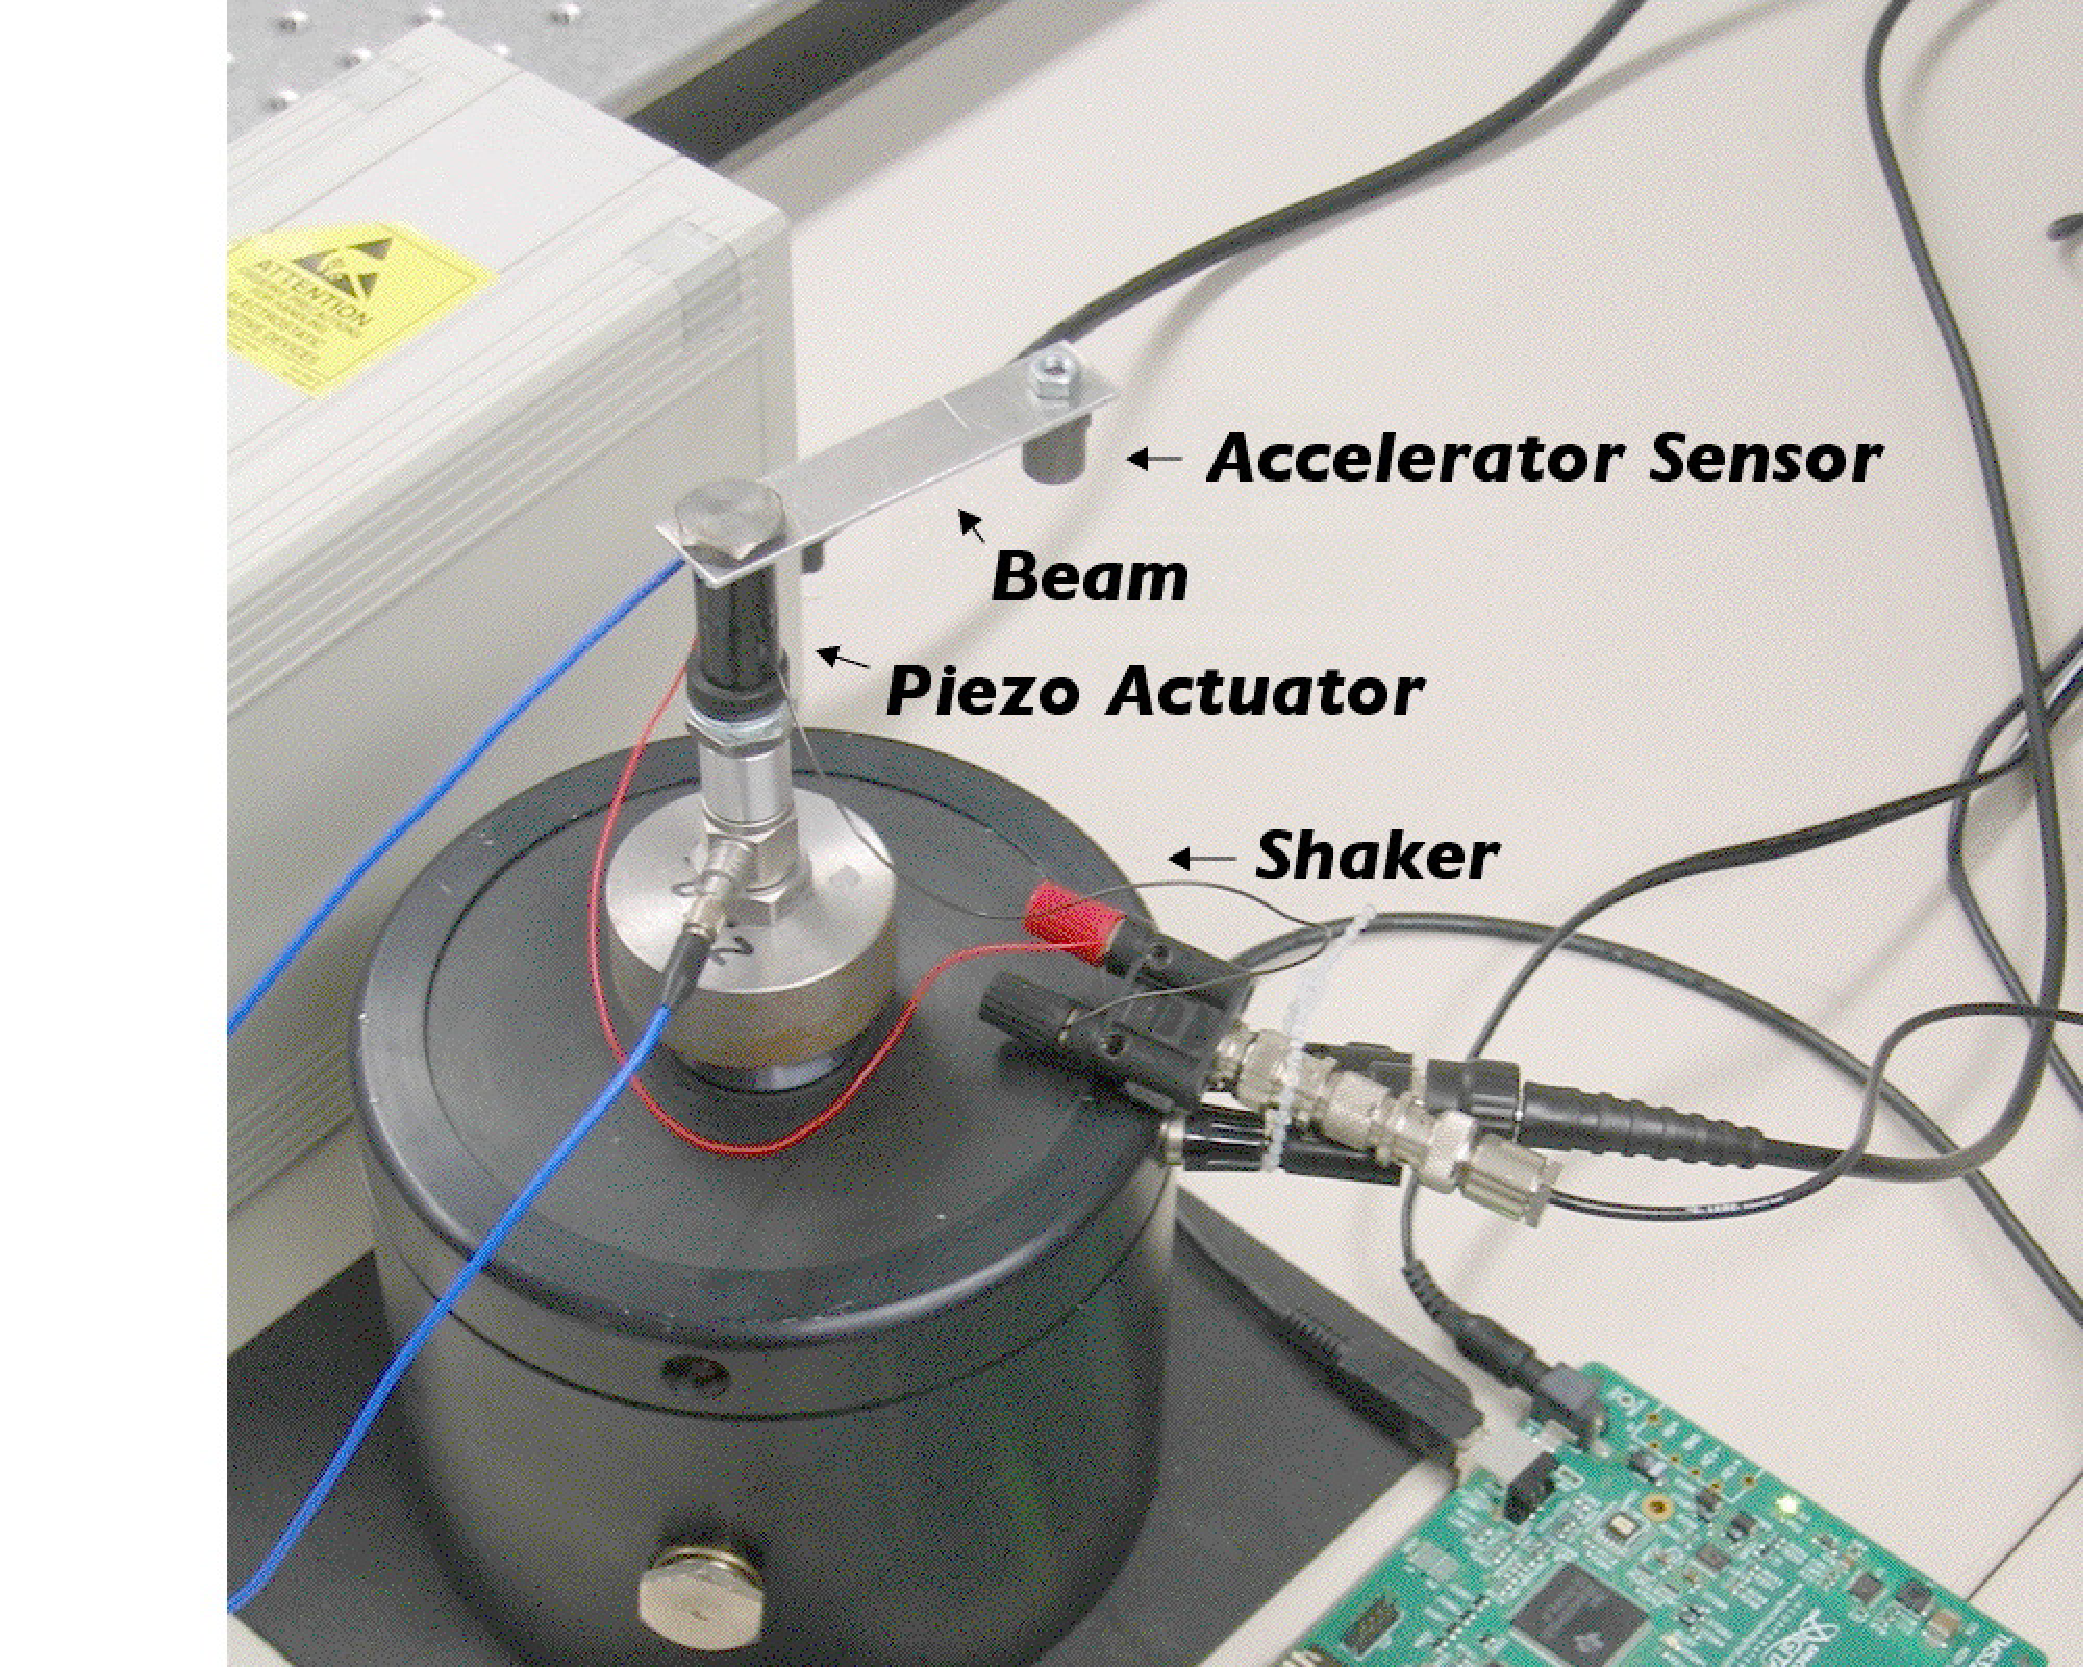
\includegraphics[scale=0.25]{../pdf/beam}
\caption{{\bf Piezo experiment}\label{beam}}
\label{default}
\end{center}
\end{figure}
The goal is to control  the actuator
using an adaptive FxLMS filter in order to dampen the resultant vibration of the beam. 

An adaptive FxLMS filter is determined by the following components:
\begin{center}
   \setlength{\unitlength}{0.9pt}   
   \begin{picture}(280,90)
   \put(-2,45){\footnotesize $x(n)$}
   \put(0,58){\vector(1,0){110}}
   \put(20,58){\vector(0,1){25}}
   \put(20,58){\circle*{3}}
   \put(20,58){\line(0,-1){45}}
   \put(20,13){\vector(1,0){20}}
   \put(40,0){\framebox(40,26){$\hat{S}(z)$}}
   \put(84,0){\footnotesize $x'(n)$}
   \put(80,13){\vector(1,0){30}}
   \put(110,0){\framebox(40,26){LMS}}
   \put(135,72){\vector(1,1){12}}
   \put(130,26){\line(0,1){20}}
   \put(150,13){\line(1,0){13}}
   \put(110,45){\framebox(40,26){$W(z)$}}
   \put(155,49){\footnotesize $y(n)$}
   \put(150,58){\vector(1,0){30}}
   \put(180,45){\framebox(40,26){$S(z)$}}
   \put(225,45){\footnotesize $y'(n)$}
   \put(220,58){\vector(1,0){26}}
   \put(250,58){\circle{8}}
   \put(250,85){\vector(0,-1){23}}
   \put(254,58){\vector(1,0){30}}
   \put(275,45){\footnotesize $e(n)$}
   \put(255,75){\footnotesize $d(n)$}
   \put(270,13){\line(0,1){45}}
   \put(270,13){\vector(-1,0){120}}
   \dashline[28]{5}(35,-5)(155,-5)
   \dashline[28]{5}(35,-5)(35,90)
   \dashline[28]{5}(35,90)(155,90)
   \dashline[28]{5}(155,-5)(155,90)
 \end{picture}
\end{center} 

\begin{itemize}
\item The actor-sensor system $S$ (secondary system) is comprised of the piezo actuator, the beam, and the accelerator sensor. Under the assumption that the filter $W(z)$ is 
linear and time invariant, the filter $W(z)$ and the secondary system may be switched. 
Replacing the secondary system by its model $\hat{S}$ results in the Figure above. 
The dashed line then include the FxLMS filter algorithm.

\item The adaptive FIR filter $w(z)$ specified
 by the difference equation $$y(n) = \sum_{i=0}^N w_{i} \cdot x(n-i)$$,

\item the stochastic LMS algorithm by the equation
$$w_{i}(n+1) = w_{i}(n) + \mu \cdot x(n-i) \cdot e(n)$$
where $e(n) = d(n) - y(n)$  is the error with $d(n)$ being the sensor signal.
\end{itemize}

This algorithm is active in state \pp{controlling} of the subsequent
program (with names being more meaningful). 
%
\codeinput{fxlms}
%
\begin{figure}[htbp]
\begin{center}
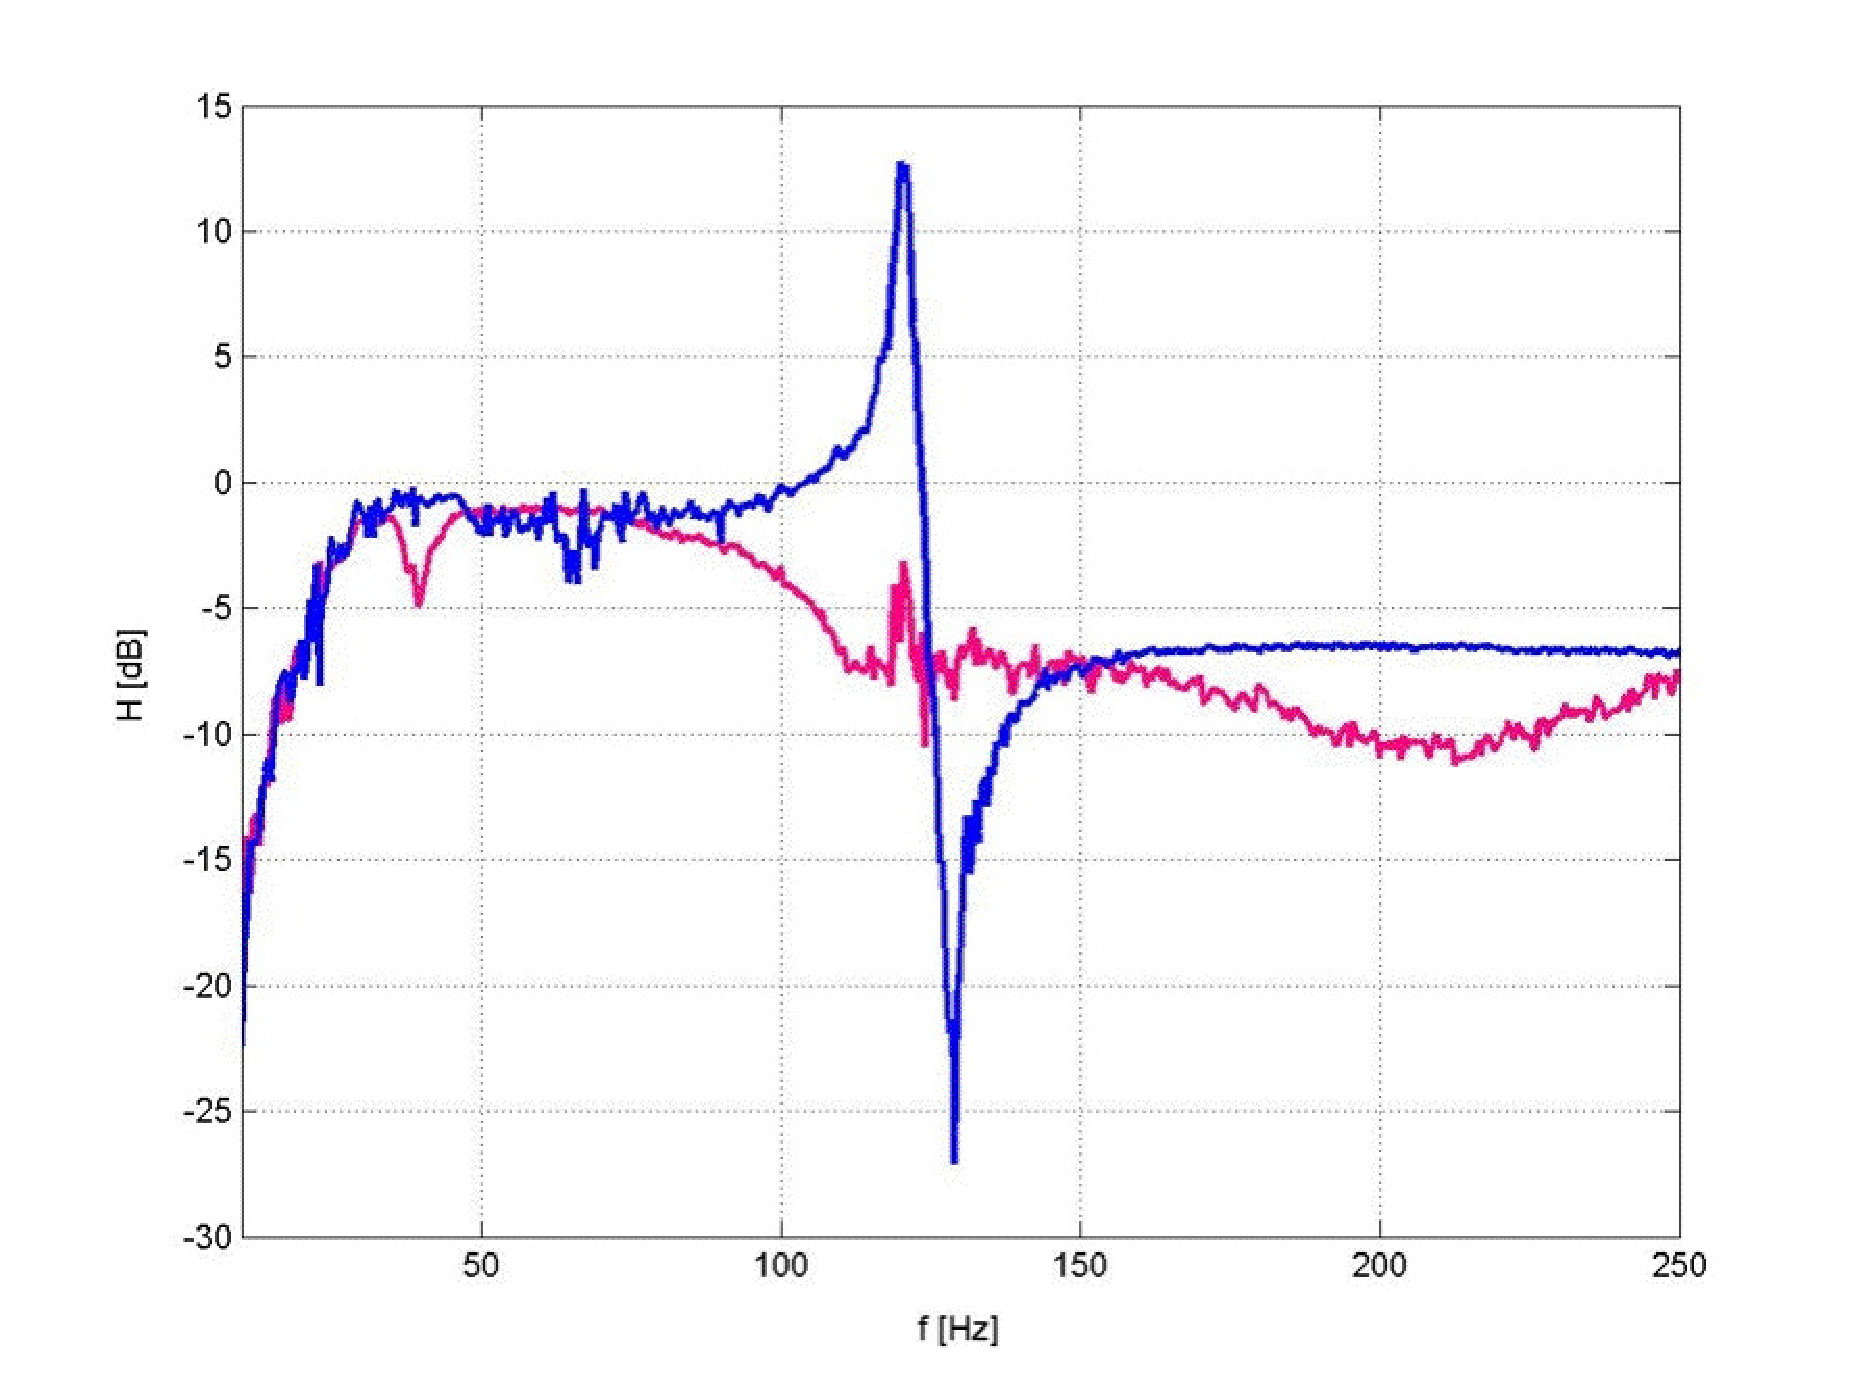
\includegraphics[scale=0.25]{../pdf/dampening}
\caption{{\bf Piezo experiment}\label{dampening}}
\end{center}
\end{figure}

There are two other states:
\begin{itemize}
  \item In state \emph{identify} system identification of the secondary
       system takes place, and

  \item in state \emph{shaker\_only} only the shaker is excited by the 
    native method \pp{noise-gen} which generates white noise. This state is meant
    provide a reference with regard controlled state in which the vibration is
    actively dampened by the piezo actuatuator. 
\end{itemize}
The results can be seen in Figure \ref{dampening}. The blue line specifies the undampened, the red line the dampened behaviour.

The program runs on a DSP evaluation board by Texas Instrument to be seen in Figure 
\ref{beam}. The board provides
a Codec and several Dip switches and Led's that are encapsulated in respective
input and output classes. The program is built and uploaded from the code as given.

\section{Representing State Models}

\paragraph{Dynamic systems a state model.} A \emph{state model} is a system of first-order coupled differential equations of the form
\begin{eqnarray*}
x'_{1} & = & f_{1}(t,x_{1},\ldots,x_{n},u_{1},\ldots,u_{p})\\
x'_{2} & = & f_{2}(t,x_{1},\ldots,x_{n},u_{1},\ldots,u_{p})\\
\vdots      &   & \vdots \\
x'_{n} & = & f_{n}(t,x_{1},\ldots,x_{n},u_{1},\ldots,u_{p})
\end{eqnarray*}
where $x'_{i}$ denotes the derivative of $x_{i}$ with regard to the time variable $t$, and $u_{1},\ldots,u_{p}$ are specified input variables. The variables $\dot(x)_{1},\ldots,\dot(x)_{n}$ are calle \emph{state variables}.


Linear time-invariant systems can easily be reformulated to a state model. Consider for instance the equations
\begin{eqnarray*}
L\frac{di(t)}{dt} +  Ri(t) + v_{c}(t)& = & v_{i}(t)
\end{eqnarray*}
and
\begin{eqnarray*}
v_{c}(t)& = & \frac{1}{C}\int_{-\infty}^td\tau
\end{eqnarray*}
describing an \textit{RLC}-circuit. Using the state variables $x_{1}(t) = i(t)$
 and $x_{2}(t) = v_{c}(t)$ substitution plus a few algebraic laws, we obtain
  the corresponding state model:
\begin{eqnarray*}
x'_{1} & = & \frac{R}{L}x_{1} + \frac{1}{L}x_{2} + \frac{v_{i}}{L}\\
x'_{2} & = & \frac{1}{C}x_{1}
\end{eqnarray*}

State models are quite a convenient representation for the numerical solution
of a system of differential equations on a computer. The method appropriate
for our purposes is the (forward) Euler method. Let 
\begin{eqnarray*}
\mathbf{x}'(t) & = & f(t,\mathbf{x},\mathbf{u})
\end{eqnarray*}
be a state mode (where $\mathbf{x}$ and $\mathbf{u}$ are vectorts). We replace the derivative by the difference approximation 
\begin{eqnarray*}
\mathbf{x}'(t) & \equiv & \frac{\mathbf{x}(t + dt)-\mathbf{x}(t)}{dt}
\end{eqnarray*}
which yields the formula
\begin{eqnarray*}
\mathbf{x}(t + dt) & \equiv & \mathbf{x}(t) + f(t,\mathbf{x},\mathbf{u})dt
\end{eqnarray*}
We can compute the estimates using the scheme
\begin{eqnarray*}
\mathbf{x}_{n+1} & \equiv & \mathbf{x}_{n} + f(t_{n},\mathbf{x}_{n},\mathbf{u}_{n})dt
\end{eqnarray*}
which naturally tranlates to \se. This is the \emph{(forward) Euler} method.

Similarly the \emph{backward Euler} method using
\begin{eqnarray*}
\mathbf{x}'(t) & \equiv & \frac{\mathbf{x}(t)-\mathbf{x}(t - dt)}{dt}
\end{eqnarray*}
for approximation can be used.

\paragraph{State models in \se.} We adopt the notation in that we allow ``primed'' signals in flow equations, e.g.
\BEP
  x1' := R/L * x1 + 1/L * x2 + vi/L\\
  x2' := 1/C * x1
\EEP
These equations will be a convenient shorthand for
\BEP
  x1 := pre(x1) + (R/L * x1 + 1/L * x2 + vi/L) * dt;\\
  x2 := pre(x2) + (1/C * x1) * dt;
\EEP
Note that this corresponds to backwards Euler. This is the more flexible
approach since we use the same scheme for
\BEP
  x1' := R/L * x1 + 1/L * pre(x2) + pre(vi)/L\\
  x2' := 1/C * x1
\EEP
to obtain forward Euler.

\paragraph{The bouncing ball example reconsidered.} We remember that the behaviour of a bouncing ball can graphically specified by the hybrid system
\begin{center}
	{\tt\small
       \thinlines
       \setlength{\unitlength}{0.9pt}
       \begin{picture}(140,100)
           \put(5,70){$x_{1} \leq 0$}
           \put(90,70){$x_{2} := -cx_{2}$}
           \put(65,76){\circle{50}}
           \put(79,59){\thicklines\vector(-2,-1){7}}
          \put(30,0){\Ovalbox{\begin{Beqnarray*}
                                      \\\ \dot{x_{1}} & = & x_{2}\
                                      \\\dot{x_{2}} & = & -g\\
                                 \end{Beqnarray*}}}       
       \end{picture}
     }
\end{center}
Hence one is tempted to translate this to
%
\codeinput{bouncing-ball-state-model-1}
%
However, this is not quite what we want since, according to the above,
the state equations translate to
\BEP
  x1 := pre(x1) + x2 * dt;\\
  x2 := pre(x2) + (-c * pre(x2) -> -g * dt;
\EEP
But the equations should be (cf. \ref{hybrid-system})
\BEP
  x1 := pre(x1) + pre(x2)* dt;\\
  x2 := (-c * pre(x2) -> x2) + -g * dt;  $(*)$
\EEP

For convenience, we add some notation which achieves just what is wanted
%
\codeinput{bouncing-ball-state-model-2}
%
Here the \pp{=>} indicates that the switch of in the previous value of the
signal. The corresponding equation $(*)$ is generated by preprocessing from
\pp{x2' := -c2 * x2 => -g}.




%Control engineers use \emph{signal flow graphs} for modelling processes.
%For instance,
%\begin{center}
%    {\footnotesize \setlength{\unitlength}{0.6pt}
%      \begin{picture}(190,120)
%	\thinlines \put(95,15){\circle*{10}} \put(140,15){\vector( -1,
%	0){40}} \put(145,15){\circle*{10}} \put(95,15){\vector( 0,
%	1){40}} \put(145,60){\vector( 0, -1){40}} \put(0,60){\vector(
%	1, 0){40}} \put(45,60){\circle*{10}} \put(50,60){\vector( 1,
%	0){40}} \put(95,60){\circle*{10}} \put(100,60){\vector( 1,
%	0){40}} \put(145,60){\circle*{10}} \put(150,60){\vector( 1,
%	0){40}} \put(45,105){\circle*{10}} \put(45,60){\vector( 0,
%	1){40}} \put(95,105){\circle*{10}} \put(50,105){\vector( 1,
%	0){40}} \put(95,105){\vector( 0, -1){40}}
%	\put(22,75){\makebox(0,0)[lb]{$z^{-1}$}}
%	\put(120,0){\makebox(0,0)[b]{$-b_1$}}
%	\put(180,65){\makebox(0,0)[b]{$y$}}
%	\put(70,65){\makebox(0,0)[b]{$a_0$}}
%	\put(5,65){\makebox(0,0)[b]{$x$}}
%	\put(70,110){\makebox(0,0)[b]{$a_1$}}
%	\put(172,32){\makebox(0,0)[rb]{$z^{-1}$}}
%      \end{picture}}
%\end{center}
%presents a recursive filter of first degree.  The values of ingoing
%arcs are added up, and the result is dispatched to the outgoing arcs.
%The labels are coefficients, $z^{-1}$ is time shifting operator for
%delaying by one unit of time.

%The signal flow graph is a presentation of the difference equation
%% 
%$$y(n) = a_0 * x(n) + a_1 * x(n-1) - b_1 * y(n-1),$$
%% 
%with the time index $n \in I\!\!N_o$ and the initial condition $y_0 = 
%a_{0} * x(t_{0})$.

%

%
%\section{More Examples}
%

%\subsection{A Lift Controller}

%A lift moves and stops while reacting to requests caused by pressing buttons. There are three kinds of buttons, \emph{lift} buttons, and \emph{up} and \emph{down} buttons. The 
%lift buttons are in the lift.\footnote{The example solution is 
%a transcription of a Lustre program designed by Leslek Holenderski~\cite{holenderski}.}

%\subsection{The Production Cell}

%Leszeks example









\chapter{Reuse}\label{reuse}

Up to this point, the aspect of control dominates the exposition. We 
have essentially been interested in the reactive code. The 
foundations of synchronous programming are settled by now, and we can 
proceed to a more structural, object-oriented view. 

\section{Interfacing Reactive Objects.}\label{signalbus}
\index{object!reactive}\index{reactive object}

\paragraph{Parameterizing reactive classes.} We reiterate that 
reactive objects communicate by sensors and signals only.  
The interface to the environment has been discussed in in Section~\ref{interface}. Now we focus on interfacing reactive objects. 

Sensors and signals are passed to reactive object by calling
its constructor. Note that reactive objects have only one constructor. 
To give an example, we modify 
the class \pp{Counter} of Subsection~\ref{counter} of 
Chapter~\ref{core}: the sensors and signals become parameters of the
constructor
% 
\codeinput{counter-object}
% 
Instances of reactive classes are created using the operator \pp{new} 
as usual.  Counters are, for instance, used in the class 
\pp{PulseWidthModulation} to modulate a signal \pp{wave} to be ``up'' 
and ``down'' for a specified number of instants.
%
\codeinput{pulse-width-modulation1}
% 
The signal \pp{wave} is emitted with value \pp{true} if the value 
\pp{toHighPhase} is present, and emits the signal \pp{wave} with 
value \pp{false} if the value \pp{toHighPhase} is present. The 
counter \pp{highTimer} counts the instants of the high phase, as 
specified by the actual value of the variable \pp{high}, and the 
counter \pp{lowTimer} counts the instants of the low phase, as 
specified by the actual value of the variable \pp{low}.

The signals \pp{clock}, \pp{toHighPhase}, and to \pp{toLowPhase} are
arguments of the two constructors of the counters. One should note 
that the signals are constrained to be read-only sometimes. For 
instance, the signal \pp{toHighPhase} is restricted to be read-only 
as argument of the counter initializing \pp{highTimer} (since the 
parameter \pp{start} of the counter if of type \pp{ConstSignal}). In 
contrast, the counter initializing \pp{lowTimer} emits the signal 
\pp{toHighPhase} but can only read the signal \pp{toLowPhase}. 

\paragraph{Constructor invocations.}\index{constructor!invocation} The semantics of object 
composition is that, when generating an instance of class 
\pp{PulseWidthModulation}, 
\begin{itemize}
\item signal parameters are substituted by arguments, e.g. the 
signal parameter \pp{start} of a counter is substituted by the signal 
argument \pp{toHighTimer} when initialising of the 
variable \pp{highTimer}.

\item the reactive code of the object \pp{PulseWidthModulation} and of
all its reactive subobjects -- here the two counters 
\pp{highTimer} and \pp{lowTimer} -- are put in parallel.
\end{itemize}

The resulting reactive code is (more or less) equivalent to
%
\codeinput{pulse-width-modulation2}
% 
Some renaming has been used: for instance, the method \pp{reset} of the
class \pp{Counter}  has two  ``localised'' versions \pp{resetHigh} and \pp{resetLow} to mimic the objects \pp{highTimer} and \pp{lowTimer}.


\paragraph{Objects and Multiple Emittance}\index{precedences, signals and objects}

Since reactive objects evaluate in parallel, and since they may share signals, conflicts may arise due to multiple emittance. Consider the following (rather useless) object
%
\codeinput{multiple-emittance1}
% 
which is instantiated twice
%
\codeinput{multiple-emittance2}
% 
Hence the signal \pp{result} is emitted twice at the first instant, with the value $3$ and with value $5$. An error message \pp{MultEmitInAppl} is raised. Since the error concerns several objects, precedence rules as defined so far will fail to cope. We introduce a new kind of precedence is introduced:
%
\codeinput{multiple-emittance3}
%
It states that if the signal \pp{result} is emitted in both the objects \pp{simple1} 
and \pp{simple2}, the \emph{every} emittance of the signal in \pp{simple1} precedes
any emmittance of the signal in \pp{simple2}.



\section{The Signal Bus}\index{signal bus}
\paragraph{Pictorial presentation.} If we focus on the reactive part 
of objects, a pictorial presentation may be illuminating. Let an 
instance of the class \pp{Counter} be sketched by
\begin{center}
   \setlength{\unitlength}{0.9pt}   
   \begin{picture}(160,90)
   \put(0,0){\framebox(160,80)}
   \put(10,10)
   {\small
   \begin{picture}(140,65)

      \put(25,70){\vector(0,-1){35}}
      \put(0,60){\scriptsize\texttt{start}}
      \put(60,70){\vector(0,-1){35}}
      \put(35,60){\scriptsize\texttt{clock}}
      \put(110,35){\vector(0,1){35}}
      \put(115,44){\scriptsize\texttt{elapsed}}
       
      \put(10,0)
       {\begin{picture}(120,35)
          \put(35,15){\scriptsize\textit{reactive code}}
          \dashline[28]{5}(0,0)(120,0)
          \dashline[28]{5}(0,0)(0,35)
          \dashline[28]{5}(0,35)(120,35)
          \dashline[28]{5}(120,0)(120,35)
       \end{picture}}
   \end{picture}}
 \end{picture}
\end{center}
Its reactive code is indicated by the dashed box, and the object 
itself by the framed box (forgetting about data fields and methods) 
The parameter signals are presented by arrows going from the framed 
box to the dashed box and vice versa.

The reactive structure of an instance of class 
\pp{PulseWidthModulation} may be then presented by
\begin{center}
\begin{picture}(335,135)
\put(0,0){\framebox(335,130)}

 \put(10,80){\line(1,0){315}} 
 \put(10,90){\line(1,0){315}} 
 \put(10,100){\thicklines\vector(1,0){325}} 
 \put(0,110){\thicklines\line(1,0){325}} 
 \put(1,110){\thicklines\vector(1,0){5}} 
 \put(0,120){\thicklines\line(1,0){325}} 
 \put(1,120){\thicklines\vector(1,0){5}} 
 \put(10,122){\footnotesize clock}
 \put(10,112){\footnotesize start}
 \put(305,102){\footnotesize wave}
 \put(100,92){\scriptsize toHighPhase}
 \put(220,82){\scriptsize toLowPhase}
 
 \put(20,110){\vector(0,-1){60}}
 \put(30,90){\vector(0,-1){40}}
 \put(40,80){\vector(0,-1){30}}
 \put(70,50){\vector(0,1){50}}

 \put(127,90){\vector(0,-1){46}}
 \put(150,120){\vector(0,-1){76}}
 \put(185,44){\vector(0,1){40}}

 \put(247,80){\vector(0,-1){36}}
 \put(270,120){\vector(0,-1){76}}
 \put(305,44){\vector(0,1){46}}

\put(5,5){\tiny PulseWidthModulation}

\put(5,5) {
 \begin{picture}(335,140)
       \put(0,0) {\scriptsize
       \begin{picture}(120,35)
          \put(15,25){\textit{reactive code}}
          \dashline[28]{5}(0,10)(80,10)
          \dashline[28]{5}(0,10)(0,45)
          \dashline[28]{5}(0,45)(80,45)
          \dashline[28]{5}(80,20)(80,45)
       \end{picture}}
            
  \put(80,0){
   \setlength{\unitlength}{0.7pt}
   \tiny
   \begin{picture}(160,110)  
   
   \put(0,0){\framebox(160,90)}
   \put(10,10)
   {\tiny
   \begin{picture}(140,65)
      \put(10,10)
       {\begin{picture}(120,35)
          \put(30,15){\scriptsize\textit{reactive code}}
          \dashline[28]{5}(0,0)(120,0)
          \dashline[28]{5}(0,0)(0,35)
          \dashline[28]{5}(0,35)(120,35)
          \dashline[28]{5}(120,0)(120,35)
       \end{picture}}
    \end{picture}}
    \put(5,5){highTimer}
  \end{picture}}
 \put(200,0){
   \setlength{\unitlength}{0.7pt}
   \tiny
   \begin{picture}(160,110)  
   
   \put(0,0){\framebox(160,90)}
   \put(10,10)
   {\tiny
   \begin{picture}(140,65)
      \put(10,10)
       {\begin{picture}(120,35)
          \put(30,15){\scriptsize\textit{reactive code}}
          \dashline[28]{5}(0,0)(120,0)
          \dashline[28]{5}(0,0)(0,35)
          \dashline[28]{5}(0,35)(120,35)
          \dashline[28]{5}(120,0)(120,35)
       \end{picture}}
    \end{picture}}
    \put(5,5){lowTimer}
  \end{picture}}
 \end{picture}}
\end{picture}
\end{center}
The picture suggests that the reactive codes of the objects involved 
are executed in parallel and that the different fragments of code 
communicate via a bundle of signals. We speak of a \emph{signal bus} 
to refer to this bundle. The signal bus is comprised of all signal 
(fields) specified in a class. We distinguish local signals such as 
\pp{toHighPhase} and \pp{toLowPhase}, input signals such as 
\pp{clock} and \pp{start}, and output signals such as \pp{wave}. We 
distinguish input and outputs to the environment by a thicker line, 
and indicate the interface to the environment by connecting them to 
the vertical sides of the framed box (while parameter signals are 
connected to the top of the box). 

The \se-logo\index{\se-logo}
\begin{center}
    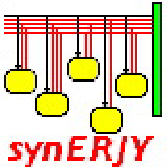
\includegraphics[width=40pt]{../pdf/se-logo}    
\end{center}
is meant to visualize the idea of a \emph{signal bus}.


%We may give an UML object diagram of the same configuration which 
%tells less, though.
%\begin{center}
%   {\tt\scriptsize
%   \setlength{\unitlength}{0.9pt}
%   \begin{picture}(370,190)

%   \put(0,75){\framebox(60,40){\underline{:PulseW\ldots}}}
%   \put(40,115){\vector(1,1){60}} 
%   \put(40,75){\vector(1,-1){60}} 
%   \put(15,120){\tiny highTimer}
%   \put(15,65){\tiny lowTimer}

%   \put(55,115){\vector(2,1){125}} 
%   \put(55,120){\tiny toHighPhase}   
%   \put(60,98){\vector(3,1){120}} 
%   \put(80,110){\tiny start}   
%   \put(60,95){\vector(1,0){120}} 
%   \put(90,97){\tiny clock}   
%   \put(60,92){\vector(3,-1){120}} 
%   \put(80,78){\tiny wave}   
%   \put(55,75){\vector(2,-1){125}} 
%   \put(55,68){\tiny toLowPhase} 
%   
%   \put(100,160){\framebox(40,30){\underline{:Timer}}}
%   \put(100,0){\framebox(40,30){\underline{:Timer}}}   
%   
%   \put(140,15){\vector(1,4){40}} 
%   \put(130,50){\tiny start}   
%   \put(140,175){\vector(1,-4){40}} 
%   \put(130,140){\tiny start}   
%   \put(140,5){\vector(1,0){40}} 
%   \put(142,0){\tiny elapsed}   
%   \put(140,185){\vector(1,0){40}} 
%   \put(142,187){\tiny elapsed}   
%   \put(140,10){\vector(1,2){40}} 
%   \put(144,175){\tiny clock}   
%   \put(140,180){\vector(1,-2){40}} 
%   \put(144,13){\tiny clock}   
%   
%   
%   \put(180,160){\framebox(80,30){\underline{:Signal}}}
%   \put(180,120){\framebox(80,30){\underline{:ConstSignal}}}
%   \put(180,80){\framebox(80,30){\underline{:ConstSignal}}}
%   \put(180,0){\framebox(80,30){\underline{:Signal}}}
%   \put(180,40){\framebox(90,30){\underline{:Signal<boolean>}}}
%   \put(260,135){\vector(1,0){30}} 
%   \put(260,95){\vector(1,0){30}} 
%   \put(270,55){\vector(1,0){20}} 
%   
%   \put(290,120){\framebox(50,30){\underline{:Input}}}
%   \put(290,80){\framebox(50,30){\underline{:Input}}}
%   \put(290,40){\framebox(50,30){\underline{:Output}}}

% \end{picture}}
%\end{center}
%We see that all the signals of an object of type 
%\pp{PulseWidthModulation} 
%are aliased with signals of the respective subobjects. This is how 
%the 
%wiring of signals is presented from the object-oriented perspective. 

  
\paragraph{Signal bus hierarchy.} Reactive objects and signal busses 
naturally form hierarchies.\index{hierarchy}\index{signal bus!hierarchy}
 Consider, for instance, a variant of the 
\pp{Counter} class.
%
\codefragment{counter-parameter-fragment}
%
Here the parameters are used to initialize the signals \pp{start}, 
\pp{clock}, and \pp{elapsed}. The corresponding graphics is
\begin{center}
   \begin{picture}(160,110)
   \put(13,93){\scriptsize\texttt{\_start}}
   \put(40,100){\vector(0,-1){20}}
   \put(58,93){\scriptsize\texttt{\_clock}}
   \put(85,100){\vector(0,-1){30}}
   \put(105,93){\scriptsize\texttt{\_elapsed}}
   \put(140,60){\vector(0,1){40}}
   
   \put(0,0){\framebox(160,100)}
   \put(10,10)
   {\small
   \begin{picture}(140,65)
      \put(0,50){\line(1,0){140}} 
      \put(0,60){\line(1,0){140}} 
      \put(0,70){\line(1,0){140}}

      \put(25,70){\vector(0,-1){35}}
      \put(0,64){\scriptsize\texttt{start}}
      \put(60,60){\vector(0,-1){25}}
      \put(35,54){\scriptsize\texttt{clock}}
      \put(110,35){\vector(0,1){15}}
      \put(115,44){\scriptsize\texttt{elapsed}}
       
      \put(10,0)
       {\begin{picture}(120,35)
          \put(35,15){\scriptsize\texttt{loop \{ \ldots\ \};}}
          \dashline[28]{5}(0,0)(120,0)
          \dashline[28]{5}(0,0)(0,35)
          \dashline[28]{5}(0,35)(120,35)
          \dashline[28]{5}(120,0)(120,35)
       \end{picture}}
   \end{picture}}
 \end{picture}
\end{center}
The signal bus is comprised of the signal fields that are used inside 
the reactive code and that are connected to the parameters. Using 
this kind of counter the composition of objects yields the following 
hierarchy where each object has a local signal bus.\index{signal bus!local}
\begin{center}
\begin{picture}(335,140)
\put(0,0){\framebox(335,130)}

 \put(10,80){\line(1,0){315}} 
 \put(10,90){\line(1,0){315}} 
 \put(10,100){\thicklines\vector(1,0){325}} 
 \put(0,110){\thicklines\line(1,0){325}} 
 \put(1,110){\thicklines\vector(1,0){5}} 
 \put(0,120){\thicklines\line(1,0){325}} 
 \put(1,120){\thicklines\vector(1,0){5}} 
 \put(10,122){\footnotesize clock}
 \put(10,112){\footnotesize start}
 \put(305,102){\footnotesize wave}
 \put(100,92){\scriptsize toHighPhase}
 \put(220,82){\scriptsize toLowPhase}
 
 \put(20,110){\vector(0,-1){60}}
 \put(30,90){\vector(0,-1){40}}
 \put(40,80){\vector(0,-1){30}}
 \put(70,50){\vector(0,1){50}}

 \put(127,90){\vector(0,-1){29}}
 \put(150,120){\vector(0,-1){66}}
 \put(185,47){\vector(0,1){33}}

 \put(247,80){\vector(0,-1){19}}
 \put(270,120){\vector(0,-1){66}}
 \put(305,47){\vector(0,1){33}}

\put(5,5){\tiny PulseWidthModulation}

   
\put(5,5) {
 \begin{picture}(335,140)
       \put(0,0) {\scriptsize
       \begin{picture}(120,35)
          \put(15,25){\textit{reactive code}}
          \dashline[28]{5}(0,10)(80,10)
          \dashline[28]{5}(0,10)(0,45)
          \dashline[28]{5}(0,45)(80,45)
          \dashline[28]{5}(80,10)(80,45)
       \end{picture}}
            
  \put(80,0){
   \setlength{\unitlength}{0.7pt}
   \tiny
   \begin{picture}(160,110)  
   
   \put(0,0){\framebox(160,90)}
   \put(10,10)
   {\tiny
   \begin{picture}(140,65)
      \put(0,50){\line(1,0){140}} 
      \put(0,60){\line(1,0){140}} 
      \put(0,70){\line(1,0){140}} 

      \put(25,70){\vector(0,-1){35}}
      \put(0,64){\texttt{start}}
      \put(60,60){\vector(0,-1){25}}
      \put(35,54){\texttt{clock}}
      \put(110,35){\vector(0,1){15}}
      \put(115,44){\texttt{elapsed}}
       
      \put(10,0)
       {\begin{picture}(120,35)
          \put(20,15){\scriptsize\textit{reactive code}}
          \dashline[28]{5}(0,0)(120,0)
          \dashline[28]{5}(0,0)(0,35)
          \dashline[28]{5}(0,35)(120,35)
          \dashline[28]{5}(120,0)(120,35)
       \end{picture}}
    \end{picture}}
    \put(1,1){highTimer}
  \end{picture}}
 \put(200,0){
   \setlength{\unitlength}{0.7pt}
   \tiny
   \begin{picture}(160,110)  
   
   \put(0,0){\framebox(160,90)}
   \put(10,10)
   {\tiny
   \begin{picture}(140,65)
      \put(0,50){\line(1,0){140}} 
      \put(0,60){\line(1,0){140}} 
      \put(0,70){\line(1,0){140}} 

      \put(25,70){\vector(0,-1){35}}
      \put(0,64){\texttt{start}}
      \put(60,60){\vector(0,-1){25}}
      \put(35,54){\texttt{clock}}
      \put(110,35){\vector(0,1){15}}
      \put(115,44){\texttt{elapsed}}
       
      \put(10,0)
       {\begin{picture}(120,35)
          \put(20,15){\scriptsize\textit{reactive code}}
          \dashline[28]{5}(0,0)(120,0)
          \dashline[28]{5}(0,0)(0,35)
          \dashline[28]{5}(0,35)(120,35)
          \dashline[28]{5}(120,0)(120,35)
       \end{picture}}
    \end{picture}}
    \put(1,1){lowTimer}
  \end{picture}}
 \end{picture}}
\end{picture}
\end{center}
The pictures are meant to suggest that
\begin{itemize}
  \item reactive objects and signal busses form a static hierarchy, 
and that

  \item if signals of different busses are "wired" together, it is 
sufficient to generate only one signal (we refer to as 
\emph{principal signal}\index{signal!principal}) and to replace every signal by its principal 
signal.
\end{itemize} 
We will analyse these requirements more deeply in 
Section~\ref{firewalls}.

\paragraph{Configuration classes.} 
Reactive classes without parameters are considered as potential configuration classes. A configuration class\index{configuration class}\index{class!configuration} generates an executable in that itself and all the reactive classes below in the static hierarchy of reactive classes are ``wired'' are wired to form one application.

A configuration class must be chosen explicitly if there is more than one candidate (using a combobox in the \se\ programming environment). A configuration class must be chosen explicitly if there is more than one candidate (using a combobox In the \se\ programming environment \cite{userguide})).

One should note that candidates for a configuration class may be below each other within the static hierarchy.


\paragraph{On input and output signals.} 
We like to stress that every reactive object may specify input sensors\index{sensor!input} and output signals\index{signal!output}. This is in contrast to the more usual idea that input and output signals are defined only top-level
by the configuration object (i.e. the only object generated by a configuration class).


There are good reasons: imagine an application with some component 
being a key pad for submitting a personal identification number.  The 
design of such pads may vary, even in terms of the number of inputs.  
However, the number of inputs usually is irrelevant with regard to 
the overall application that may only depend on whether a correct pin 
has been submitted. 

A schematic view of the key pad control in terms of the interface may 
be
\begin{center}
  \begin{picture}(180,120)
    \put(0,0){\framebox(180,110){}}
    \put(5,68){\footnotesize accept}
    \put(1,65){\thicklines\vector(1,0){5}}
    \put(0,65){\thicklines\line(1,0){170}}
    \put(5,78){\footnotesize bn}
    \put(1,75){\thicklines\vector(1,0){5}}
    \put(0,75){\thicklines\line(1,0){170}}
    \put(3,85){\ldots}
    \put(5,98){\footnotesize b1}
    \put(1,95){\thicklines\vector(1,0){5}}
    \put(0,95){\thicklines\line(1,0){170}}
    \put(150,58){\footnotesize receipt}
    \put(10,55){\thicklines\vector(1,0){170}}
    \put(63,103){\footnotesize reset}
    \put(85,110){\vector(0,-1){70}}    
    \put(100,103){\footnotesize pin}
    \put(95,40){\vector(0,1){70}}    

    \put(40,95){\vector(0,-1){55}} 
    \put(50,75){\vector(0,-1){35}} 
    \put(60,65){\vector(0,-1){25}} 
    \put(140,40){\vector(0,1){15}}    
    
    \put(30,5)
     {\begin{picture}(120,35)
        \put(35,15){\small\textit{reactive code}}
        \dashline[28]{5}(0,0)(120,0)
        \dashline[28]{5}(0,0)(0,35)
        \dashline[28]{5}(0,35)(120,35)
        \dashline[28]{5}(120,0)(120,35)
     \end{picture}}

  \end{picture}    
\end{center}
Here \pp{pin} is meant to be a integer valued signal. The 
box/reactive 
object analyses the sequence of pressed keys if an \pp{accept} 
is submitted. If the sequence is submitted the pin is communicated to 
the application, and the \pp{receipt} signal is emitted with an OK 
message, 
otherwise only the \pp{receipt} signal is emitted with an reject 
message. The number of keys is irrelevant for the overall 
application. It depends on the actual pad. Typically it will have ten 
keys, for instance, for an electronic bank till but there might be 
other builds. 

If input and output signals can only be specified at top-level one 
may have to touch many components of an application to pass the 
key signals down to the pin analyser and to pass the receipt signal 
back to top-level. In \se, these variations have only a local impact 
in 
that the component and the connectors have to be redesigned. In that 
the rationale of \se\ is component oriented in that reactive objects 
behave the same within an application even if the interface to the 
environment may differ.


\section{Structural Constraints}\label{firewalls}\index{firewall}

\paragraph{Firewalls for separating concerns.} A design goal of \se\ 
has been clearly to separate of different concerns as there are: 
reactive control, data operations, and interaction of objects. We 
speak of \emph{firewalls} if addressing these separations of 
concern.  The firewalls encapsulate some of the design decision of 
\se. There are three such firewalls:
\begin{description}
    \item[] \emph{Data Firewall}
     -- Control dominates data.

    \item[] \emph{Signal Firewall}
    -- Reactive object only share 
signals. 

%    \item[] \emph{State Firewall} -- Only state information is 
%communicated in distributed synchronous systems.
\end{description}
%The latter will be explained only later in Chapter~\ref{dsp}. 

\paragraph{The data firewall.}
\index{firewall!data}\index{data firewall}
The data firewall avoids dynamic changes of the reactive control.  The
data firewall restricts the use relation in that
\begin{itemize}
    \item A reactive class can only be a subclass of a reactive 
class. 
    
    \item data methods cannot invoke reactive methods.
\end{itemize}
The requirement reflects the standard two-level architecture for 
control  applications: control dominates data.

\paragraph{The signal firewall.}
\index{firewall!signal}\index{signal firewall}
The signal firewall constrains time race analysis of data calls to 
reactive objects, both for reasons of transparency and for reasons of 
efficiency of the semantic analysis. The constraints are that
\begin{itemize}
     \item constructor parameters are either primitive types
     and signal types, and that
    
     \item all fields and methods of a reactive class are private.
\end{itemize}
The combination avoids that two reactive objects can share 
data except for signals.

Note that time races may still occur between signal emittances.  Like
causality, time races can only partly be resolved on the level of a 
class but requires an analysis at the level of an application, at some 
cost in terms of computing time for the semantic analysis.

\paragraph{Control is static.}
\index{staic control}\index{control!static}
 The firewalls are effective due to an 
essential fact: the structure of reactive behaviour is statically 
determined at compile time. Only then our analysis of causality and 
of time races is feasible. Control is static because of several 
constraints.
\begin{itemize}
	\item For each reactive class, the call graph of reactive methods
	is cycle-free.

	\item The call graph of reactive objects forms a tree with the
	configuration object at the root (i.e. the one having the method
	\pp{main}).
    
	\item Subtrees of objects are downwards closed with regard to
	signals: an reactive object can access signals of a super object,
	but not vice versa, i.e. \emph{the signal bus must be properly
	constructed}.

    \item Reactive objects do not share data except for signals.
\end{itemize}

\paragraph{Mapping the signal bus.} 
Using constructor parameters for sharing signals is too general to
implement the signal bus faithfully.  For the signal bus, we have to
guarantee that there is exactly one signal that corresponds to one
wire.

For a proper implementation of the signal bus\index{signal bus!implementation}, a signal variable  
must be constrained to refer to a signal of the following kinds:
\begin{itemize}
    \item  a \emph{local} signal, or

    \item  an \emph{input} or \emph{output} signal,

    \item  a \emph{global} signal of a super object.
\end{itemize}
We speak of local and input/output signals as \emph{principal
signals}\index{signal!principal}
 of the respective object. By induction, a global signal is a 
principal signal of some super object. 

This constraint is syntactically enforced by requiring that
\begin{enumerate}
    
	\item a signal can be assigned to only once. 
    
    \item the assignment to a signal only occurs in its declaration or
    in a constructor tail.  A \emph{constructor tail}
    \index{constructor!tail} consists of a
    sequence of (unconditional) signal assignments followed by
     the active statement.

    \item an assignment to a signal variable is either of the forms
    \begin{quote}
        \texttt{\textit{signal\_variable} = new
        \textit{signal\_constructor}(\ldots);}\\
        \texttt{\textit{signal\_variable} = 
\textit{formal\_parameter};}
    \end{quote}

    \item a signal constructor only occurs in an assignment or
    initializer of the form
    \begin{quote}
        \texttt{\ldots\ \textit{signal\_variable} = new
        \textit{signal\_constructor}(\ldots);}
    \end{quote}
    In that case we refer to \textit{signal\_variable} as a
    \emph{principal signal}\index{signal!principal}.
 
\end{enumerate}
Condition 1 states that at most one value can be assigned to a signal
(variable).  Conditions 2 and 3 state that
\begin{itemize}
    \item a signal (variable) is either initialized using class
    instance generation (\pp{new \ldots}) (this is a principal signal)
    \emph{principal signal}, or that

    \item a signal being argument of the constructor is assigned to
    a signal variable.
\end{itemize}
By induction, every signal argument of a constructor is the principal
signal of some super object.  Hence every signal variable refers to
principal signals, which faithfully reflects the signal wiring of the
visual presentation.  Finally, condition 4 guarantees that ``all
signals are principal''; all signal (objects) are refered to by a
signal (variable).

\section{\textit{A Loophole in the Signal 
Firewall}}\label{trespassing}\index{firewall!loophole}\index{loophole}
{\em

\paragraph{\textit{An example}} In spite of the signal firewall, 
there might be a time race of data methods being invoked in different 
objects. Consider a configuration consisting of a ``sender'' and a ``receiver'' 
\codefragment{Sender}
\codefragment{Receiver}
The configuration class just establishes a connection between a 
sender and two receivers.  
\codefragment{Signalbus}
The class \emph{\pp{Data}} has just a field \emph{\pp{value}} that 
can be updated.
\codefragment{Data}

The behaviour is thus: at the first instant, \emph{\pp{sender}}
\begin{enumerate}
	\item[1.] updates the fields of \emph{\pp{data}} to $0$ ,

	\item[2.]  emits the shared signal \emph{\pp{sig}} with value 
	\emph{\pp{data}}, and

    \item[3.]  updates the fields \emph{\pp{val}} of 
\emph{\pp{data}} to
    $3$. 
\end{enumerate}
In parallel,
\begin{enumerate}
	\item[4.] \emph{\pp{receiver1}} updates the fields of 
\emph{\pp{data}}  	to $1$, and
	\item[4.] \emph{\pp{receiver2}} updates the fields of 
\emph{\pp{data}}  	to $2$.
\end{enumerate}
In contrast to what we aim for, there are time races between the 
various invocations of the method \pp{set}.
 
\paragraph{\textit{Dealing with the problem.}} 
Signals with values of class type allow to transmit complex data 
which clearly is a useful feature. The prize to pay is time races
may occur across object borders.

There are several strategies of how to avoid such time races. Remember once
a signal is updated, its value should not change any more, but only be read 
(\emph{write-before-read}). This trivially holds for values primitive 
type. For values of class type, one should only be able to access
its fields but not to change them. The same holds for arrays.

In other languages than \java\ this is achieved using a class modifier \pp{const} that defines a superclass comprising only those methods 
that are read-only. Hence emittance of signal with a value of class type
should emit a copy obtained by the respective ``const''\index{const} type. 
In that case the three applications of the method \pp{set} would 
be illegal. However, it would be legal to apply to replace the line
\BEP
\$sent.set(3):
\EEP
of the class \pp{Sender} by the line
\BEP
data.set(3):
\EEP
without changing semantic content. 

An alternative strategy would be to guarantee by an in-depth data analysis
that a signal value is not changed once the signal has been emitted/constrained.

Neither of these strategies is currently implemented in \se. Hence we must
leave it as an \textbf{obligation for the programmer} to pursue either of the
strategies:
\begin{itemize}
\item Either explicitly to design ``const'' classes without side effects,
 and to restrict signal values to these, 

\item or otherwise to guarantee that signal value is not changed after emittance.
\end{itemize}

}


%\section{Abstract Reactive Classes}
%A class is reactive if
%\begin{itemize}
%    \item  it has a reactive constructor, i.e. the constructor tail 
%            of the form
%           \begin{center}
%				\pp{active \{ \ldots\ \}},
%            \end{center}
%    \item  it comprises a signal declaration (cf. this section), or

%    \item  a reactive methods (cf. Section~\ref{methods}).

%    \item  the modifier \pp{reactive} is used. (cf. Section~\ref{methods}).
%\end{itemize}
%If a reactive class does not have a reactive constructor it is an {\em abstract reactive class}. The idea is that a reactive class may inherit signal declarations and reactive methods without being ``executable''. Since we expect that an instance of a reactive class generates reactive code, and since reactive code is only generated from within the \pp{active} statement it seems reasonable to consider reactive classes without an reactive constructor as abstract; no instances can be generated. 

%Here is a small example

%\ldots

%Abstract reactive classes are particularly useful in the context of data flow. As discussed in Chapter~\ref{data-flow} data flow specifications are modularized using nodes as  building blocks. Typically data flow specifications share such building blocks that are elementary (such as the raising edge node). All these elementary nodes -- and, of course, others which are shared -- may be zusamenfassen in some abstract reactive class from which other reactive classes inherit. E.g.

%\section{Examples}

%%\subsection{A Traffic Light Controller}

%

%\subsection{A Production Cell}

%\paragraph{The setup.} The production cell consists of a robot that 
%assembles parts as in Figure~\ref{fallstudie}. The case study has 
%been proposed in \cite{kowalewski}.
%\begin{center}
%\begin{figure}[h]
%  \includegraphics[width=280pt]{../pdf/atp-production-cell}
%  \caption{The Production Cell}
%  \label{fallstudie}
%\end{figure}% 
%\end{center}

%\paragraph{The components.}
%Figure~\ref{fallstudie} suggests to consider the robot, the conveyor belt,
%and the storage as components that are complemented by a central control. 

%We now have to decide  which components are considered as being part of
%the control system, and which components are considered as being 
%part of the environment (plant), the latter being only needed to close
%the system for simulation. We here take the view that the storages and
%the central control are part of the system while the robot and the belt
%are part of the environment. The decision is temporary and may be revised
%at any time. We first model the components of both, the system and the environment.
% 
%\paragraph{The storage.}
%The storage is modelled by a class \pp{Stock} as below
%%
%\codeinput{atp-stock}
%%
%The reactive behaviour consists of two parallel processes. The upper
%one models book-keeping. This, being a sort of continuous 
%behaviour, is best modelled using the flow equations. 
%Parts can be added or withdrawn. A sensor \pp{newPart} checks for
%the presence of a new part. If it is present we increase the stock.
%On the other hand, the stock is decreased if a part is withdrawn by
%the robot. 

%
%Einem Lager k\"{o}nnen Teile hinzugef\"{u}gt oder entnommen werden. 
%Dies modellieren wir in Kode 3 mit Hilfe von Datenfl\"{u}ssen, da die
%Information kontinuierlich berechnet wird.  Dazu passt die 
%Vorstellung
%eines Datenflusses als Sequenz von Werten.

%In einer Datenflussgleichung wird f\"{u}r alle Takte definiert, dass
%die Flussvariable auf der linken den Wert des Ausdrucks auf der
%rechten Seite hat.  So beschreibt zum Beispiel der Fluss \pp{lager}
%die Zahl der gelagerten Montageteile.  Diese ist im ersten Takt $0$
%und wird in sp\"{a}teren Takten aus der Zahl der Teile im vorigen 
%Takt
%(\pp{pre(lager}) sowie den Zu- und Abg\"{a}ngen im jetzigen Takt
%berechnet.\footnote{Wie in \textsc{Lustre}~\cite{lustre} wird auf 
%der linken
%Seite des Operators \pp{->} das Verhalten im ersten Takt, auf der
%rechten Seite das Verhalten in sp\"{a}teren Takten beschrieben.} Der
%Boolesche Fluss \pp{geliefert} wird wahr, wenn im vorigen Takt eine
%Entnahmeanforderung vorlag und das Lager gef\"{u}llt war.  Der Fluss
%\pp{weg} ist gleich dem konstanten Fluss \pp{1..}, wenn ein Teil
%geliefert wurde, und dem Fluss \pp{0..} sonst.  Integer-Konstanten
%werden durch den Operator \pp{..} zu einem konstanten Integer-Fluss. 
%F\"{u}r eine kompakte Darstellung benutzen wir den aus C
%gel\"{a}ufigen Operator \pp{{\it\normalsize c} ?{\it\normalsize t}
%:{\it\normalsize e}} anstelle eines ``\pp{if{\it\normalsize c}
%then{\it\normalsize t} else{\it\normalsize e}}''.

%Der Fluss \pp{platzVoll} zeigt an, ob ein
%Montageteil auf dem Greifplatz liegt.
% 
%\BEP
%  sustain \{
%      hinzu      := (?neuesTeil..) ? (1..) : (0..);
%      geliefert  := pre(?entnahme.. \& lager > 0..);
%      weg        := (geliefert) ? (1..) : (0..);
%      lager      := 0.. -> pre(lager) + hinzu - weg;
%      platzVoll  := lager > 0.. \& geliefert;
%  \};

%\mbox{\footnotesize {\bf
%Kode 3:} Lagerhaltung}
%\EEP
%  
%Sporadisches und kontinuierliches Verhalten wird in dem Beispiel
%kombiniert; wir gehen von der Vorstellung aus, dass ein neu
%produziertes Teil beim Eintritt in das Lager durch eine Lichtschranke
%erkannt wird.  Dieses spontane Ereignis wird durch das Signal
%\pp{neuesTeil} modelliert und durch \pp{?neuesTeil..} f\"{u}r
%die weitere Verarbeitung zu einem Fluss konvertiert.  Dagegen
%l\"{a}sst sich der Zustand \pp{platzVoll} des Greifplatzes eleganter
%durch einen Booleschen Fluss beschreiben, obwohl das Verhalten auf 
%den
%ersten Blick \"{a}hnlich erscheint.

%Die Modellierung ist noch unrealistisch; der Greifplatz bleibt nur
%einen Takt leer.  Wenn wir davon ausgehen, dass kein Sensor f\"{u}r
%den Greifplatz verf\"{u}gbar ist, ist die Annahme sinnvoller, dass 
%der
%Greifplatz erst nach Ablauf einer gewissen Zeitspanne wieder besetzt
%sein kann.  Diese Abstraktion l\"{a}\ss t sich elegant imperativ als
%reaktives Verhalten parallel zum Datenfluss formulieren (Kode 4).
% 
%\BEP
%  [[ sustain \{
%       \ldots
%       platzVoll  := lager > 0.. \& \$zeitVorbei..;
%     \};
%  || loop \{
%       await (\$lager > 0);
%       await fuellZeit;
%       emit zeitVorbei(true);
%       await (\$geliefert);
%       emit zeitVorbei(false);
%     \};
%  ]];

%\mbox{\footnotesize {\bf
%Kode 4:} Lagerhaltung}
%\EEP

%

%

%\paragraph{The signal bus.}
%Figure~\ref{signalbus} specifies the layout of the signal bus of the control system. 
%\begin{center}
%\begin{figure}[h]
% {\tt
%     \setlength{\unitlength}{1.4pt}   
% \begin{picture}(240,100)
%    \put(5,90){\bf Control}
%    \put(30,70){\thicklines \vector(0,-1){30}} 
%    \put(30,40){\thicklines \vector(0,1){30}} 
%    \put(5,10){\framebox(50,30){\it active}}
%    \put(75,100){\vector(0,-1){30}} 
%    \put(78,75){\small\texttt{part}}
%    \put(145,100){\vector(0,-1){30}} 
%    \put(110,75){\small\texttt{beltSpeed}}
%    \put(175,70){\vector(0,1){30}} 
%    \put(178,93){\small\texttt{problem}}
%    \put(10,70){\thicklines \line(1,0){240}} 
%    \put(0,0){\thicklines\framebox(260,100)}
%    \put(100,70){\vector(0,-1){30}} 
%    \put(46,45){\small cPartWithdrawn}    
%%    \put(100,23){\footnotesize withdrawal}    
%    \put(105,40){\vector(0,1){30}} 
%%    \put(110,35){\vector(0,1){5}} 
%    \put(107,62){\small cPartAvailable} 
%%    \put(110,35){\footnotesize partAvailable}    
%    \put(70,25){\vector(1,0){25}}     
%    \put(60,17){\small c.newPart}
%    \put(95,10){\thicklines\framebox(50,30){}}
%    \put(97,22){\small\bf Stock cParts}
%    \put(197,70){\vector(0,-1){30}} 
%    \put(143,45){\small dPartWithdrawn}    
%%    \put(200,28){\footnotesize withdrawal}    
%    \put(202,40){\vector(0,1){30}} 
%    \put(203,62){\small dPartAvailable}    
%    \put(170,25){\vector(1,0){25}}     
%%    \put(205,35){\footnotesize partAvailable}    
%    \put(160,17){\small d.newPart}
%    \put(195,10){\thicklines\framebox(50,30){}}
%    \put(197,22){\small\bf Stock dParts}
% \end{picture}}
%  \caption{The Signal Bus}
%  \label{signalbus}
%\end{figure}
%\end{center}
%The reactive object \pp{control} has two sub-objects \pp{cParts} and \pp{dParts} of type \pp{Stock} that model the respective stocks. 

%A stock
%has parameter \pp{withdrawn}, being a sensor, and a parameter \pp{partAvailable} being a signal. 

%The signals \pp{cPartWithdrawn} and \pp{cPartAvailable} replace the parameters  
%Dieser besteht aus einem B\"{u}ndel von
%Signal(leitung)en, das durch die dickere Linie angedeutet wird.  Die
%Signale des Busses k\"{o}nnen in dem aktiven Teil der Steuerung
%gelesen oder geschrieben werden.  Zum B\"{u}ndel geh\"{o}rige Signale
%wie \pp{cEntnahme} und \pp{cGreifPlatzVoll} werden dem Konstruktor 
%der
%Klasse \pp{Lager} mitgegeben, um ein Lager in seine Umgebung
%einzupassen.  Die Modularisierung in \se\ l\"{a}sst also sowohl
%abgeschlossene Komponenten als auch deren hierarchische Verfeinerung
%zu.

%Man beachte, dass jedes reaktive Objekt mit Hilfe lokaler Signale
%\"{u}ber Eingabe- und Ausgabeobjekte mit der Umgebung kommunizieren
%kann.  So k\"{o}nnen die Lager \pp{c} und \pp{d} unmittelbar 
%\"{u}ber die lokalen Signale \pp{c.neuesTeil}  und \pp{d.neuesTeil} 
%angesprochen werden. Diese Lokalit\"{a}t der Ein- und Ausgabe 
%erh\"{o}ht 
%die Flexibilit\"{a}t des Entwurfs.

%

%
%Wir m\"{u}ssen diese (didaktisch hilfreiche) Fehlentscheidung
%zur\"{u}cknehmen und werden anstelle des Attributs ein Signal
%\pp{problem} verwenden.  Wir ersetzen in dem Kode der Steuerung (Kode
%1) den Aufruf der Methode \pp{setProblem(x)} durch ein \pp{emit 
%signal(x)} und fragen in der Bandeinheit ab, ob ein Problem vorliegt

%\BEP
%loop {
%   emit problem(NO\_PROBLEM);
%   emit bandTempo(100); // motor full speed :-)
%   await \$problem != NO\_PROBLEM;
%   next;
%   emit bandTempo(0);   // turn motor off
%   next;
%   await ?restart;      // problem solved
%};

%\mbox{\footnotesize {\bf
%Kode 6:} Revision von Kode 1}\EEP

%Damit haben wir eine saubere Trennung der avisierten Komponenten 
%erzielt. 

%
%\paragraph{Modelled by a state machine: the assembling line.}
%The robot and the conveyor belt interact for assembling the parts. 
%According to which part arrives either a part of type $C$ or $D$ has 
%to be taken. We specify control in terms of a simple state machine 
%having the states  
%\begin{description}

%\item[``\pp{wait}'':] If a part of type \pp{A} or \pp{B} is arriving then 
%move either to state \pp{assemble\_C} or \pp{assemble\_D}.  Otherwise 
%issue an error message.

%\item[``\pp{assemble\_C}'':] If  there is a part at grab point C,
%  a message is issued that a part has been taken (\pp{cPartTaken}) and that 
%  it is to be assembled (\pp{assembled(\$part)}), and the automaton
%  moves to state \pp{wait}. Otherwise it is checked
%  whether the conveyor belt stand still. If not, an error message is issued  
%  \pp{problem(Status.NO\_PART\_C)}. In any case, the state \pp{assemble\_C}
%  is reentered. The error message is meant to stop the movement of the belt.
%  The assumption that the belt does not need to be stopped for assembling
%  if the appropriate part is available.
%  
%    \item[``\pp{assemble\_D}'':]  analogously
%\end{description}

%The corresponding automaton is specified below. Note that identifiers in
%capital letters such as \pp{PART\_A} oder \pp{MISSING\_C} denote constants. 
%%
%\codefragment{atp-control}
%% 

%We use strong abstractions here. For instance, we indicate the behaviour 
%of the robot by emission of the signal \pp{assembled} only. This is 
%sufficient for a first design, and may be refined later. one might think of 
%reformulating the state \pp{assemble\_C} to
%\BEP
%    state assemble\_C
%       entry \{ emit startRobot(\$part); \}
%       when (?assembled) \{           
%          next state wait; 
%       \} else \ldots
%\EEP
%The signal \pp{startRobot} is emitted when entering state
%\pp{assemble\_C} in which control remains until 
%the robot indicates success by emitting the signal \pp{assembled}.

%The assembly line is encapsulated as an object

%\paragraph{Modelled by an imperative program: the belt control.}

%The conveyor belt is controlled by
%%
%\codefragment{atp-belt-control}
%%
%By emmitting the signal \pp{beltSpeed} the intended speed of
%the belt is set. We assume that an internal controller of the
%belt controls the belt so that it approaches the required 
%speed. Again we use an abstraction. Such a controller may later be designed (for instance, as a PID controller using data flow).
%Hence if the signal \pp{beltSpeed(100)} the motor is accelerated (to full speed). If some problem occurs the belt is slowed down to stop. Then the program waits till the problem is resolved as indicated by the presence of the signal  \pp{restart}.  

%Ob ein Problem vorliegt, wird durch den Aufruf der Booleschen
%(Daten-) Methode \pp{hasProblem} entschieden.  Als Seiteneffekt wird
%dabei das Attribut \pp{problem} auf den Wert \pp{NO\_PROBLEM}
%zur\"{u}ckgesetzt.
% 
%\BEP
%  boolean hasProblem() \{
%     local int p = problem;
%     problem = NO\_PROBLEM;
%     return (p != NO\_PROBLEM);
%  \};
%\EEP
% 

%Schaltet man die beiden Programmst\"{u}cke zur Montage und
%Bandverwaltung parallel, weist der \se\ Kompilierer auf einen 
%Konflikt
%zwischen Aufrufen der Methoden \pp{setProblem} und \pp{hasProblem}
%hin.  Beide k\"{o}nnen in einem Takt gleichzeitig gerufen werden, 
%ohne
%dass die Programmstruktur eine Ablaufordnung festlegt.  Dies 
%f\"{u}hrt
%zu Nichtdeterminismus in der Auswertung.  In einem solchen Falle kann
%der Entwickler die Reihenfolge durch einen Sequenzbefehl festlegen.
% 
%\BEP
%  sequence \{
%     setProblem(int) < hasProblem();
%  \};
%\EEP
% 
%Damit wird in jedem Takt jeder Aufruf der Methode \pp{setProblem} 
%stets
%vor jedem Aufruf der Methode \pp{hasProblem} ausgef\"{u}hrt.  
%Generell
%werden nur Programme akzeptiert, bei denen alle derartige Konflikte
%aufgel\"{o}st sind.  Der erzeugte Kode ist
%deterministisch.\footnote{Der Kompilierer w\"{u}rde ein \"{a}hnliches
%Problem entdecken, wenn einer der \pp{next} Befehle vergessen worden
%w\"{a}re.  Dann k\"{o}nnte das Signal \pp{bandTempo}
%nicht-deterministisch mit dem Wert 0 oder mit dem Wert 100 emittiert
%werden.}

%\paragraph{Modelled by data flow: the storage}

%Einem Lager k\"{o}nnen Teile hinzugef\"{u}gt oder entnommen werden. 
%Dies modellieren wir in Kode 3 mit Hilfe von Datenfl\"{u}ssen, da die
%Information kontinuierlich berechnet wird.  Dazu passt die 
%Vorstellung
%eines Datenflusses als Sequenz von Werten.

%In einer Datenflussgleichung wird f\"{u}r alle Takte definiert, dass
%die Flussvariable auf der linken den Wert des Ausdrucks auf der
%rechten Seite hat.  So beschreibt zum Beispiel der Fluss \pp{lager}
%die Zahl der gelagerten Montageteile.  Diese ist im ersten Takt $0$
%und wird in sp\"{a}teren Takten aus der Zahl der Teile im vorigen 
%Takt
%(\pp{pre(lager}) sowie den Zu- und Abg\"{a}ngen im jetzigen Takt
%berechnet.\footnote{Wie in \textsc{Lustre}~\cite{lustre} wird auf 
%der linken
%Seite des Operators \pp{->} das Verhalten im ersten Takt, auf der
%rechten Seite das Verhalten in sp\"{a}teren Takten beschrieben.} Der
%Boolesche Fluss \pp{geliefert} wird wahr, wenn im vorigen Takt eine
%Entnahmeanforderung vorlag und das Lager gef\"{u}llt war.  Der Fluss
%\pp{weg} ist gleich dem konstanten Fluss \pp{1..}, wenn ein Teil
%geliefert wurde, und dem Fluss \pp{0..} sonst.  Integer-Konstanten
%werden durch den Operator \pp{..} zu einem konstanten Integer-Fluss. 
%F\"{u}r eine kompakte Darstellung benutzen wir den aus C
%gel\"{a}ufigen Operator \pp{{\it\normalsize c} ?{\it\normalsize t}
%:{\it\normalsize e}} anstelle eines ``\pp{if{\it\normalsize c}
%then{\it\normalsize t} else{\it\normalsize e}}''.

%Der Fluss \pp{platzVoll} zeigt an, ob ein
%Montageteil auf dem Greifplatz liegt.
% 
%\BEP
%  sustain \{
%      hinzu      := (?neuesTeil..) ? (1..) : (0..);
%      geliefert  := pre(?entnahme.. \& lager > 0..);
%      weg        := (geliefert) ? (1..) : (0..);
%      lager      := 0.. -> pre(lager) + hinzu - weg;
%      platzVoll  := lager > 0.. \& geliefert;
%  \};

%\mbox{\footnotesize {\bf
%Kode 3:} Lagerhaltung}
%\EEP
%  
%Sporadisches und kontinuierliches Verhalten wird in dem Beispiel
%kombiniert; wir gehen von der Vorstellung aus, dass ein neu
%produziertes Teil beim Eintritt in das Lager durch eine Lichtschranke
%erkannt wird.  Dieses spontane Ereignis wird durch das Signal
%\pp{neuesTeil} modelliert und durch \pp{?neuesTeil..} f\"{u}r
%die weitere Verarbeitung zu einem Fluss konvertiert.  Dagegen
%l\"{a}sst sich der Zustand \pp{platzVoll} des Greifplatzes eleganter
%durch einen Booleschen Fluss beschreiben, obwohl das Verhalten auf 
%den
%ersten Blick \"{a}hnlich erscheint.

%Die Modellierung ist noch unrealistisch; der Greifplatz bleibt nur
%einen Takt leer.  Wenn wir davon ausgehen, dass kein Sensor f\"{u}r
%den Greifplatz verf\"{u}gbar ist, ist die Annahme sinnvoller, dass 
%der
%Greifplatz erst nach Ablauf einer gewissen Zeitspanne wieder besetzt
%sein kann.  Diese Abstraktion l\"{a}\ss t sich elegant imperativ als
%reaktives Verhalten parallel zum Datenfluss formulieren (Kode 4).
% 
%\BEP
%  [[ sustain \{
%       \ldots
%       platzVoll  := lager > 0.. \& \$zeitVorbei..;
%     \};
%  || loop \{
%       await (\$lager > 0);
%       await fuellZeit;
%       emit zeitVorbei(true);
%       await (\$geliefert);
%       emit zeitVorbei(false);
%     \};
%  ]];

%\mbox{\footnotesize {\bf
%Kode 4:} Lagerhaltung}
%\EEP

%
%\paragraph{The overall architecture.} 

%\paragraph{Reaktive Objekte}

%Verhaltenskomponenten werden durch \emph{reaktive Klassen} 
%modelliert. 
%Eine wesentliche Einschr�nkung der so definierten reaktiven Objekte 
%ist,
%dass diese nur \"{u}ber Signale kommunizieren d\"{u}rfen.  Dies
%garantiert, dass keine Interaktion der Objekte \"{u}ber Daten 
%erfolgt.

%Ein (rudiment\"{a}res) Beispiel sei

%\BEP
%class Lager \{ 
%  time fuellZeit;
%  ConstSignal   entnahme;
%  Flow<boolean> platzVoll;
%  ConstSignal   neuesTeil  = new ConstSignal(new Input());
%  \ldots

%  public Lager (    ConstSignal \_entnahme, 
%                 Flow<boolean> \_platzVoll, 
%                          time \_fuellZeit  ) \{
%      fuellZeit = \_fuellZeit;
%      entnahme  = \_entnahme;
%      platzVoll = \_platzVoll;

%      active \{
%         \textit{Verhalten - siehe Kode 4}
%     \};
%  \};
%\}

%\mbox{\footnotesize {\bf
%Kode 5:} Klasse Lager}
%\EEP
% 
%Der Verhaltenskode wird durch die Anweisung \pp{active} in den
%Konstruktor eingebettet.  Signalvariablen werden entweder durch
%Konstruktorparameter (\pp{entnahme}) oder durch ein Signalobjekt
%(\pp{neuesTeil}) initialisiert.  An der Signalvariablen 
%\pp{neuesTeil}
%lassen weitere Besonderheiten festmachen: durch den Typ
%\pp{ConstSignal} wird festgelegt, dass das Signal nur getestet und
%nicht emittiert werden kann.  Durch den Parameter \pp{new Input()}
%wird festgelegt, dass dieses Signal mit der Umgebung kommuniziert (in
%diesem Fall als Input).

%\paragraph{Komponentenbildung}

%Reaktive Objekte verhalten sich wie Komponenten: alle Attribute und
%Methoden sind per Definition privat.  Reaktive Klassen sind nach 
%unten
%abgeschlossen.  Interaktion findet nur \"{u}ber Signale statt und
%niemals \"{u}ber Referenzen.  Damit verhalten sich reaktive
%Objekte in jeder Umgebung gleich.

%Gem�� Bild~\ref{fallstudie} bietet es sich an, die Lager und die
%Bandeinheit als Komponenten zu betrachten, die um eine zentrale
%Steuerungskomponente erg\"{a}nzt werden. Jede Komponente soll wie 
%oben 
%das Lager durch eine reaktive Klasse modelliert werden.

%Als n\"{a}chstes ist zu kl\"{a}ren, welche Komponenten wir als Teil
%des Systems und welche Komponenten wir als Teil der Umgebung
%betrachten, deren Modellierung nur dazu dient, das System f\"{u}r 
%eine
%Simulation abzuschlie\ss en.  Wir treffen hier die Entscheidung, dass
%die Lager und die Steuerung Teil des Systems, die Bandeinheit dagegen
%Teil der Umgebung ist.  Diese Entscheidung ist momentan und l\"{a}sst
%sich jederzeit revidieren, wenn wir zum Beispiel eine ausgefeiltere
%Steuerung der Bandeinheit mit dem Diskriminator und Ortsschalter
%entwickeln.

%Wir m\"{u}ssen aber nun feststellen, dass unsere bisherige
%Modellierung dieser Aufteilung nicht standh\"{a}lt; die
%Steuerung und die Bandeinheit greifen \"{u}ber die Datenmethoden auf 
%dasselbe Attribut \pp{problem} zu. Da reaktive Klassen nach unten 
%abgeschlossen sind, ist dies nur m\"{o}glich, wenn das Verhalten der 
%Steuerung und der Bandeinheit in der gleichen Klasse formuliert 
%sind. 

%Wir m\"{u}ssen diese (didaktisch hilfreiche) Fehlentscheidung
%zur\"{u}cknehmen und werden anstelle des Attributs ein Signal
%\pp{problem} verwenden.  Wir ersetzen in dem Kode der Steuerung (Kode
%1) den Aufruf der Methode \pp{setProblem(x)} durch ein \pp{emit 
%signal(x)} und fragen in der Bandeinheit ab, ob ein Problem vorliegt

%\BEP
%loop {
%   emit problem(NO\_PROBLEM);
%   emit bandTempo(100); // motor full speed :-)
%   await \$problem != NO\_PROBLEM;
%   next;
%   emit bandTempo(0);   // turn motor off
%   next;
%   await ?restart;      // problem solved
%};

%\mbox{\footnotesize {\bf
%Kode 6:} Revision von Kode 1}\EEP

%Damit haben wir eine saubere Trennung der avisierten Komponenten 
%erzielt. 

%\paragraph{Signalbus}

%Komponenten werden \"{u}ber einen sogenannten \emph{Signalbus}
%verbunden.  Die Idee ist, dass sich Signale wie Leitungen verschalten
%lassen.  So wird etwa der Boolesche Fluss \pp{cGreifPlatzVoll} der
%Montagesteuerung mit dem Fluss \pp{platzVoll} des Lagers f\"{u}r
%C-teile verbunden ebenso wie das Signal \pp{cEntnahme} mit dem Signal
%\pp{entnahme}.  Bild 2 mag dies veranschaulichen.
%\begin{figure}[h]
% {\tt
%     \setlength{\unitlength}{0.9pt}   
% \begin{picture}(240,100)
%    \put(5,90){\bf Steuerung}
%    \put(30,70){\thicklines \vector(0,-1){30}} 
%    \put(30,40){\thicklines \vector(0,1){30}} 
%    \put(5,10){\framebox(50,30){\it active}}
%    \put(75,100){\vector(0,-1){30}} 
%    \put(78,84){\scriptsize\texttt{basisTeil}}
%    \put(145,100){\vector(0,-1){30}} 
%    \put(103,93){\scriptsize\texttt{bandTempo}}
%    \put(175,70){\vector(0,1){30}} 
%    \put(178,93){\scriptsize\texttt{problem}}
%    \put(10,70){\thicklines \line(1,0){220}} 
%    \put(0,0){\thicklines\framebox(240,100)}
%    \put(105,70){\vector(0,-1){38}} 
%    \put(65,45){\scriptsize cEntnahme}    
%    \put(107,28){\tiny entnahme}    
%    \put(110,35){\vector(0,1){35}} 
%    \put(112,62){\scriptsize cGreif-}    
%    \put(112,55){\scriptsize PlatzVoll} 
%    \put(112,35){\tiny platzVoll}    
%    \put(70,25){\vector(1,0){25}}     
%    \put(65,17){\scriptsize c.neues}
%    \put(74,9){\scriptsize Teil}
%    \put(95,10){\thicklines\framebox(50,30){}}
%    \put(100,15){\bf Lager c}
%    \put(192,70){\vector(0,-1){38}} 
%    \put(153,45){\scriptsize dEntnahme}    
%    \put(195,28){\tiny entnahme}    
%    \put(197,35){\vector(0,1){35}} 
%    \put(200,62){\scriptsize dGreif-}    
%    \put(200,55){\scriptsize PlatzVoll}    
%    \put(160,25){\vector(1,0){25}}     
%    \put(200,35){\tiny platzVoll}    
%    \put(155,17){\scriptsize d.neues}
%    \put(164,9){\scriptsize Teil}
%    \put(185,10){\thicklines\framebox(50,30){}}
%    \put(190,15){\bf Lager d}
% \end{picture}}
% \caption{Die Klasse Steuerung}
% \label{fallstudie}
%\end{figure}
%Die reaktive Klasse \pp{Steuerung} hat zwei reaktive Unterobjekte
%\pp{c} und \pp{d} vom Typ \pp{Lager}.  Diese lesen von und schreiben
%auf den (lokalen) Signalbus.  Dieser besteht aus einem B\"{u}ndel von
%Signal(leitung)en, das durch die dickere Linie angedeutet wird.  Die
%Signale des Busses k\"{o}nnen in dem aktiven Teil der Steuerung
%gelesen oder geschrieben werden.  Zum B\"{u}ndel geh\"{o}rige Signale
%wie \pp{cEntnahme} und \pp{cGreifPlatzVoll} werden dem Konstruktor 
%der
%Klasse \pp{Lager} mitgegeben, um ein Lager in seine Umgebung
%einzupassen.  Die Modularisierung in \se\ l\"{a}sst also sowohl
%abgeschlossene Komponenten als auch deren hierarchische Verfeinerung
%zu.

%Man beachte, dass jedes reaktive Objekt mit Hilfe lokaler Signale
%\"{u}ber Eingabe- und Ausgabeobjekte mit der Umgebung kommunizieren
%kann.  So k\"{o}nnen die Lager \pp{c} und \pp{d} unmittelbar 
%\"{u}ber die lokalen Signale \pp{c.neuesTeil}  und \pp{d.neuesTeil} 
%angesprochen werden. Diese Lokalit\"{a}t der Ein- und Ausgabe 
%erh\"{o}ht 
%die Flexibilit\"{a}t des Entwurfs.

%\subsubsection{Schlussfolgerungen}

%Wir haben einen ersten Entwurf\footnote{Eine vollst\"{a}ndige
%Dokumentation der Fallstudie findet man unter \cite{at}} der
%Fallstudie vorgestellt und angedeutet, wie Entwurfsentscheidungen
%lokal modifiziert und verfeinert werden k\"{o}nnen.  Das grobe Modell
%ist nicht nur eine (eventuell grafische) Darstellung des Systems.  
%Sie
%ist auch ausf\"{u}hrbar und testbar.  Simulation und Regressionstests
%auf einem Arbeitsplatzrechner zeigen trotz Parallelit\"{a}t wegen des
%Determinismus synchroner Programme das gleiche Verhalten wie auf dem
%Zielrechner.

%Ob ein Nachrichtentechniker Datenfluss bevorzugt oder ob ein 
%Informatiker hierarchische Automaten benutzt, ist eine 
%Entwicklungsentscheidung, die durch die Integration der synchronen 
%Stile verborgen werden kann.



\chapter{Building Applications}\label{InputOutput}


\section{Embedding Software}

Embedded programs is in general part of a system comprised of mechanical,
electrical, and/or pneumatic components, and of one or many micro processors 
or even workstations possibly linked by a bus system such as CAN. The embedded
program must interact with these components and it have have access to the
resources of the overall system. In \se, input sensors and output signals 
provide the interface to the environment. Access to the resources is gained 
using native methods.


\subsection{Interfacing to the Environment.}
The interface of a \se\ program to the environment is defined
in terms of \emph{input sensors}\index{sensor!input} and \emph{output signals}\index{signal!output}. We recall the basic facts.

\begin{itemize}
\item A sensor is an input sensor if its constructor has an argument of
type \pp{Input}.

\item A signal is an output signal if its constructor has an argument of
type \pp{Output}.

\item \pp{Input} and \pp{Output} are marker interfaces. 

\item An implementation of the interface \pp{Input}\index{Input@\pp{Input}} requires that
two (callback) methods \pp{new\_val}\index{new\_val@\pp{new\_val}} and \pp{get\_val}\index{get\_val@\pp{get\_val}} are implemented.

For each input sensor, the Boolean method \pp{new\_val} is called at the beginning of an instant. If it returns true, the respective signal is set to 
be present, otherwise it is set to absent. 
Then, if the sensor is valued, the method \pp{get\_val} is called. It must return a value of appropriate type that is the new value of the signal.

\item An implementation of the interface \pp{Output}\index{Output@\pp{Output}} requires that
a method \pp{put\_val}\index{put\_val@\pp{put\_val}}.

For each output signal, the method \pp{put\_val} is called at the 
end of an instant. If the signal is valued it has an argument 
of appropriate type. 
\end{itemize}


\subsection{Native Methods}
Native methods\index{method!native}\index{native} are implemented in a platform-dependent language. 
We use ANSI-C as a host language since cross-compilers are available
for most platforms, in particular if restricted to the small 
subset of ANSI-C as used by the \se\ compiler. 

We have broadened the concept in that not only methods may be native, 
but also constants, and in that \se\ methods may be exported to the
host language. We have the following formats
 
\begin{itemize}
    \item The standard format is
    %
    \BEP
        void native method\_name( \ldots );
    \EEP
    %
    A method \pp{method\_name} is defined by a C function with the same name.


    \item The native method may be renamed
    %
    \BEP
        void native("method\_name") se\_method\_name( \ldots );
    \EEP
    %    
    The method \pp{se\_method\_name} is defined by the C function
    \pp{method\_name}

    \item  Methods defined in \se\ may be exported
    %
    \BEP
        void export\_to\_C method\_name( \ldots ) \{
            \ldots
        \};
    \EEP
    %
    The function \pp{method\_name} may be called in C to execute
    the method.
    
    
    \item The exported method may be renamed

    %
    \BEP
        void export\_to\_C(method\_name) se\_method\_name( \ldots ) \{
        \ldots
        \};
        \EEP
    %    
    The function \pp{method\_name} may be called in C to execute the
    method \pp{se\_method\_name} 


    \item  Constants, i.e. fields that are static and final, may be 
    imported from C or exported to C using the same modifiers as used 
    for methods. 
\end{itemize}

Whether methods or constants are imported or exported is often a
matter of taste.  However, if such constants or methods are often
changed it is probably more convenient to export since development
takes place in the same framework.  In contrast, it might be useful
 to import in order to hide details of 
implementation. 

Import and export of constants is useful in particular since \java\
lacks enumerations.  since enumerations are typically defined by a
list of constants the \se\ program and C environment should agree
about such enumeriations which is best achieved if the enumerations 
are only defined once and then imported or exported.

\section{Interfacing to the Environment}

The following example demonstrates how interfaces may be implemented using
native methods. The example can be found in\\ 
\pp{\$SE\_HOME$\backslash$target$\backslash$examples$\backslash$Blink4}.

\paragraph{Reactive behaviour.}
The reactive behaviour of the program is specified by the reactive method
%
\codefragment{blink4-rct}
%
There is an hierarchic automaton with two states \pp{select\_green} and \pp{select\_red}. The automaton changes state if the sensor \pp{select}
is present. Each of the states host an automaton. Each of these automata
toggles between emittance and non-emittance of an output signal, \pp{red\_on}
for the state \pp{select\_red}, and \pp{red\_green} for the state \pp{select\_green}. The toggle is applied if the input sensor \pp{toggle} is
present.

\paragraph{Interfaces of sensors and signals.} 
We use a very simple idea for interfacing: each of input sensors and
output signals is known in the environment by its name as a
string. This name is passed on to the environment, either for checking for
presence with \pp{new\_val}, or when calling \pp{put\_val}.

Here is the implementation for inputs
%
\codefragment{blink4-input-button}
%
Calling the constructor stores the ``button name''. The parameterless method 
\pp{new\_val} just calls a method \pp{new\_val} with the button name being
parameter. The latter method is native, the implementing function being 
\pp{getPresence}.

An object of class \pp{InputButton} is then used to initialise the signal
\pp{toggle} in
%
\codefragment{blink4-toggle}
%
Alternatively, one might have declared an object of type \pp{InputButton}
that is used in a sensor constructor as in
%
\codefragment{blink4-select}
%

For output signals, we implement the interface \pp{Output} similarly
%
\codefragment{blink4-output-led}
%
The method \pp{put\_val} essentially calls the function \pp{printStdout}
of the environment.

A variation of the theme is define the method \pp{stdOutput} on class level
and to use an anonymous class
%
\codefragment{blink4-red-on}
%
\paragraph{The method \pp{main}.}
The method \pp{main} consists of a while loop.
%
\codefragment{blink4-main}
%
The condition of the while loop is a conjunction of two conditions.
The first condition consists of the method call \pp{read\_input}.
The method is native. It ``reads'' the input sensors as we will
see when analysing the corresponding C-code below. It is called at the beginning of an instant since it is executed before the second condition is evaluated. The second condition is the familiar call of the method \pp{instant}. 

\paragraph{The native code.}

The native code specifies all the native functions.   
\BEP
\#include <stdio.h>
\#include <string.h>
\#include <ctype.h>
\#include <stdlib.h>
\#include "se.Blink4.h" /* as generated by the sE-compiler */
\EEP

For checking the presence of input sensors we have the following code

\BEP
Bool selectPresence, togglePresence;

Bool getPresence (char *s) \{
  if (strcmp(s,"select") == 0) \{
     return selectPresence;
  \} else if (strcmp(s,"toggle") == 0) \{
     return togglePresence;
  \} else \{
     fprintf (stdout,"invalid getPresence returned FALSE$\backslash$n");
     fflush (stdout);
     return FALSE;
  \};
\}
\EEP
For each input sensor, a Boolean variable is declared. The variables
encode the status; if a variable is true, the sensor is present, otherwise
it is absent.
The function \pp{getPresence} checks whether a sensor is present or not.
Its arguments is a string that is matched with the names of the input
sensors. If the argument matches a signal name its status is returned.
If no signal name matches an error message is written to \pp{stdout}.

\BEP
Bool readInput (void) \{
  selectPresence = FALSE;
  togglePresence = FALSE;
  while ( fgets(zLine,20,stdin) ) \{
    if (zLine[0] == 'q') \{
       fprintf (stdout,"exit (0)$\backslash$n");
       fflush (stdout);
       return FALSE;
    \} else if (zLine[0] == 't') \{
       togglePresence = TRUE;
    \} else if (zLine[0] == 's') \{
       selectPresence = TRUE;
    \} else if (zLine[0] == '.') \{
       return TRUE;
    \} else \{
        fprintf (stdout,"input ignored$\backslash$n");
        fflush (stdout);
    \};
  \};
  return FALSE;
\}
\EEP

\section{Interfacing with the Environment - continued}



\section{Building a Project}

The \se\ environment supports a very elementary project handling. A \emph{project}
consists of a directory that includes all the files relevant to a particular 
application such as \se\ files, \se charts files, C files, and C libs, and a particular
\emph{project resource file} \pp{.seprj} which is generated by using 
the \emph{project panel} but which may be edited by hand. 
\begin{figure}[h]
\begin{center}
    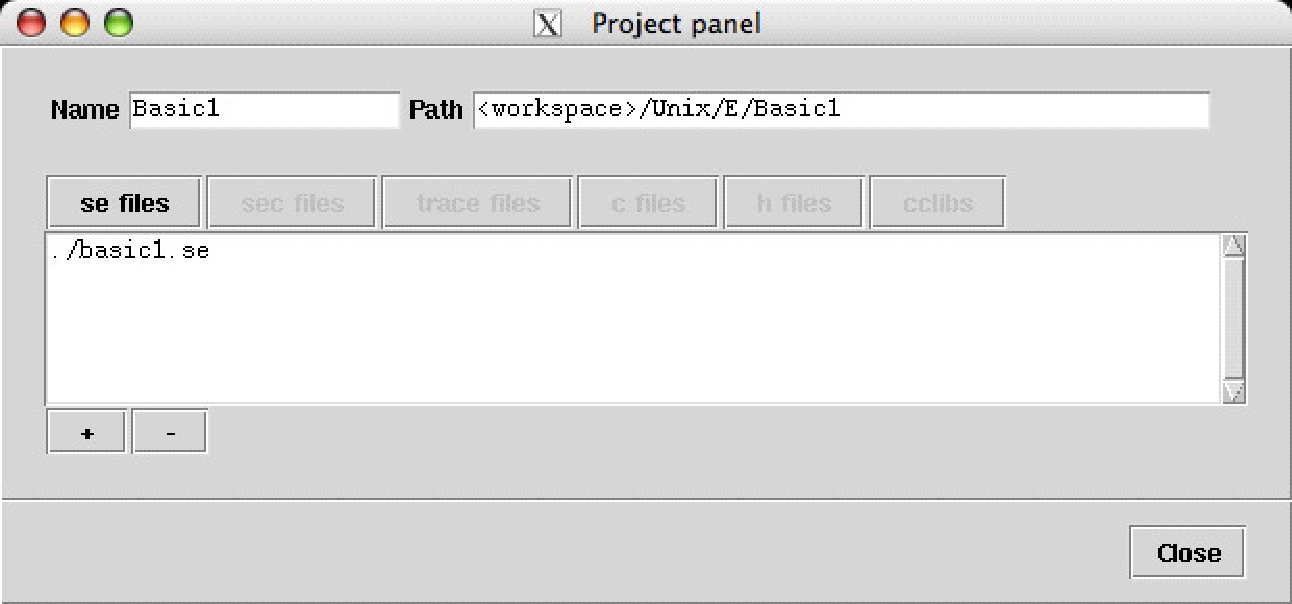
\includegraphics[width=250pt]{../pdf/synerjy-project}
\end{center}
\caption{The synERGY project panel}
\end{figure}\label{project-panel}
Here we consider the project \pp{\$SE\_HOME$\backslash$target$\backslash$examples$\backslash$Blink4} which consists of the files discussed above.

Building of an application is discussed in the \se\ user manual but a few
additional remarks may be useful. For maximal flexibility we use makefiles
for building and running an application. The \pp{Build}
button at first generates a file \pp{Makefile.gen} in \pp{\$SE\_HOME/tmp}
%
\BEP
SE\_MAKEINFO=makeinfo
SE\_WORKSPACE=/Users/ap/Unix/E/Blink4
SE\_BINARY=se.a.out
SE\_CPROGRAM=/Users/ap/Unix/E/Blink4/se.Blink4.c
SE\_CFILES=/Users/ap/Unix/E/Blink4/blink4.c 
SE\_CLIBS=
\EEP
%
in case of the example.

This file is included in a generic \pp{Makefile} in the directory
 \pp{\$SE\_HOME/target/\emph{host}}. The structure of the generic \emph{Makefile}
is as follows
%
\BEP
-include \$(SE\_HOME)/tmp/Makefile.gen

sim: 
        gcc \$(SE\_CPROGRAM) \$(SE\_CFILES) -o \$(SE\_BINARY) $\backslash$
            -Dse\_sim $\backslash$
            -Dse\_\_linux $\backslash$
            -I \$(SE\_HOME)/include $\backslash$
            -I include $\backslash$
            -I \$(SE\_HOME)/target/linux/include $\backslash$
	        \$(SE\_HOME)/target/linux/lib/libse\_rt.a $\backslash$
	        -lm -lpthread

tgt:
        gcc \$(SE\_CPROGRAM)  \$(SE\_CFILES) -o \$(SE\_BINARY) $\backslash$
	        -Dse\_\_linux $\backslash$
	        -I \$(SE\_HOME)/include  $\backslash$
	        -I \$(SE\_HOME)/target/linux/include $\backslash$
	        \$(SE\_HOME)/target/linux/lib/libse\_rt.a $\backslash$
	        -lm -lpthread

sfun:
        mex \$(SE\_CPROGRAM)  \$(SE\_CFILES) -output \$(SE\_BINARY) $\backslash$
            -Dse\_\_linux $\backslash$
            -I\$(SE\_HOME)/include $\backslash$
            -I\$(SE\_HOME)/target/linux/include $\backslash$
            \$(SE\_HOME)/target/linux/lib/libse\_rt.a

run:
        exec xterm -e \$(SE\_BINARY)

clean:
        rm -f \$(SE\_PREFIX)*
\EEP
%
There are several rules according to target.
\begin{itemize}
\item[\pp{sim}] A rule to invoke the simulator.

\item[\pp{tgt}] A rule to generate code for the host machine.

\item[\pp{sfun}] A rule to generate an Sfunction for import to Simulink.

\item[\pp{run}] A rule to run the application. Here it is executed in a terminal.
For microprocessors, this typically implies upload.

\end{itemize}

The Makefiles may be replaced according to one's taste but be careful to use the
same rules names if the \se\ environment is to be used. The better alternative
is to include a self-defined Makefile in the project directory. This will
then be called automatically instead of the predefined ones.


\section{Using Makefiles only.}

The final alternative for the friends of the hard-core approach is to use
Makefiles exclusively forgetting about soft programming environments: there
is a reasobly exprissive command language to deal with most problems on the
level of command lines or - for comfort - in a Makefile. Here is an example

\BEP
include \$SE\_HOME/target/unix/include/Makefile.inc

\# example blink4.se needs external C
now: se.Blink4

se.Blink4.c: blink4.se
	se -f "%load file=blink4.se; $\backslash$
               set target=linux;set hfile=se\_rt.h; $\backslash$
               make C-code;quit;"

se.Blink4: se.Blink4.o blink4.o
	\$(CC) -o se.Blink4 se.Blink4.o blink4.o $\backslash$
              \$(SE\_HOME)/target/unix/lib/libsert.a

\# misc stuff ******************************************************
doc: clean
	doxygen

clean:
	rm -f se.* *.o
	rm -rf html rtf man latex
	rm -rf se.*
	rm -rf sim/se.*
	rm -rf target/se.*
\EEP
The \pp{Makefile.incl} sets several variables in a uniform way. The general strategy of writing Makefiles is to  use one rule to execute two steps
\begin{itemize}
\item
generate the \pp{se.<ConfigurationClass>.c} file from the synERJY-sources
(as it is done in the \pp{se.Blink4.c} - rule)

\item
compile and link the application (as it is done in the \pp{se.Blink4} rule)

\end{itemize}

%\section{An Interface for LEGO Mindstorms}

%To be written
%% ?????????

%\section{A Microprocessor Example}

%To be written
%% ?????????

%\section{A CAN bus example}

%To be written
%% ?????????









\chapter{Validation}\label{validation}

\paragraph{A Priori}

It is a matter of a long lasting discussion what benefits may be
expected by validation techniques.  We adhere to the pragmatic point
of view that any kind of validation, let it be verification or testing, increases our confidence that a program might be reasonably well behaved.  

Validation means that we demonstrate that the behaviour of a program
complies with some sort of specification, let it be a formal 
specification in terms of some logic or a test set. Any inconsistency 
between specification and behaviour reaveals some missing 
understanding of what either the specification expresses, or how the 
program behaves. By experience, both may be wrong. Even if the program 
satisfies the specification absence of errors is not guaranteed.
Both may follow the same lines of thought generating the same mistakes.
However, independently designed specifications provide a different 
view of a problem, even if the program and the specification is 
designed by the same person. In that validation is added value.

\se\ supports formal verication of essentially the control structure
of programs using model checking (Section~\ref{verification}),  
and it supports testing on a yet rudimentary
basis.
(Section~\ref{testing}).

\section{Formal Verification by Model Checking}\label{verification}

\paragraph{The principle.} The goal of formal verification to prove an assertion $\phi$ for a given program. As an example we consider a part of a trivial controller
for traffic light. 
\BEP
  loop \{
    [[ await ?button;    // \textit{demand to cross by a pedestrian} 
    || emit car\_to\_green;
       await 30sec;     // \textit{car has a green light for > 30sec}
    ]];
    emit car\_to\_yellow;
    await 3sec;        // \textit{time for cars to clear the road}   
    emit car\_to\_red;
    await 3sec;        // \textit{safety delay}
    emit ped\_to\_green;
    await 20sec;        // \textit{Time for pedestrians to cross}
    emit ped\_to\_red;
    await 5sec;        // \textit{safety delay}   
    emit car\_to\_yellow;
    await 2sec;        // \textit{safety delay};
\EEP
Now we would like to check, for example,
\begin{enumerate}
    \item[(i)]  that the traffic light for both cars and pedestrians are
    never green at the same time (\emph{Safety condition}), or

	\item[(ii)] whether the pedestrian light eventually turns green after
	the button has been pressed. (\emph{Liveness condition}).

	\item[(iii)] the light always eventually turns green. (\emph{Liveness condition}).
\end{enumerate}

There are a number of methods to provide answers to such questions.
Pragmatically one has to consider that (i) such methods should be 
sufficiently efficient and that (ii) they should be
applicable for a non-specialist. It seems that from today's viewpoint
\emph{Model Checking }~\cite{Clarke} best complies with both these
requirements.

Model checking checks whether an assertion holds with regard to a particular
model. In case of a program as above this means that an assertion must
hold in any state that can be reached when executing the program. The 
reachable states of the piece of code above are given by the following
diagram (omitting the emitted signals)
\begin{center}
    {\tt 
     \tiny  
     \setlength{\unitlength}{0.8pt}
     \thinlines    
        \begin{picture}(210,100)
            \put(0,10){\circle{14}}
            \put(-4,9){gr}
            \put(5,12){\vector(1,0){36}}
            \put(12,0){>30sec}
            \put(0,55){\vector(0,-1){36}}
            \put(-30,35){?button}
            \put(50,10){\circle{14}}
            \put(62,0){>30sec}
            \put(55,10){\vector(1,0){40}}
            \put(50,55){\vector(0,-1){40}}
            \put(20,35){?button}
            \put(100,10){\circle{10}}
            \put(105,10){\vector(1,0){40}}
            \put(0,60){\circle{10}}
            \put(5,60){\vector(1,0){40}}
            \put(12,50){>5sec}
            \put(50,60){\circle{10}}
            \put(110,0){>3sec}
            \put(150,10){\circle{10}}
            \put(155,10){\vector(1,0){40}}
            \put(162,0){>20sec}
            \put(200,10){\circle{10}}
            \put(210,30){>5sec}
            \put(200,10){\circle{10}}
            \put(200,15){\vector(0,1){70}}
            \put(200,90){\circle{10}}
            \put(100,95){>2sec}
            \put(195,90){\line(-1,0){195}} 
            \put(0,90){\vector(0,-1){25}}            
      \end{picture}
    }
\end{center}
We indicate the status of the light by the combination of ``r'' and ``g'' in
the circles where car light is on the left and the pedestrian light on the right: e.g. ``gr'' states that the car light is green and the pedestrian light
is red. If we believe that that diagram above gives a fair account of what
the piece of program does, then a simple inspection seems to show that never both the lights are green. Similarly, it seems to be obvious that pedestrians never get ``starved''. However, in a big system such inspection is hardly manageable and asks for automation.

Actually, if we would apply model checking we would find that assertion (i) is
violated. Though the visual inspection seems to prove the assertion, the picture does not tell about initialisation: both traffic lights may be green when starting execution of the code fragment. Prefixing with 
\BEP
  emit car\_to\_red;
  emit ped\_to\_red;
\EEP 
fixes this problem. However then cars may get starved when the pedestrian button is never pressed. Changing the program structure slightly hopefully helps:
\BEP
  emit car\_to\_red;
  emit ped\_to\_red;
  loop \{
    await 5sec;        // \textit{safety delay}   
    emit car\_to\_yellow;
    await 2sec;        // \textit{safety delay};
    [[ await ?button;    // \textit{demand to cross by a pedestrian} 
    || emit car\_to\_green;
       await 30sec;     // \textit{car has a green light for > 30sec}
    ]];
    emit car\_to\_yellow;
    await 3sec;        // \textit{time for cars to clear the road}   
    emit car\_to\_red;
    await 3sec;        // \textit{safety delay}
    emit ped\_to\_green;
    await 20sec;        // \textit{Time for pedestrians to cross}
    emit ped\_to\_red;
\EEP
  
Model checking automatically constructs the space of reachable states and
checks whether a formula or a set of formulas holds in every state. If
this is not the case, a counter example is provided in terms of a trace.
Model checking really got off the ground since efficient symbolic techniques
have been developed which allow to analyse systems of industrial size.

There are restrictions, however: 
\begin{itemize}
\item Firstly, assertions are restricted to use Boolean
variables only, though recently systems are on the market that deal with
enumerations or even integers. 
\item Secondly, the complexity may grow exponentially with the size of the 
model and the assertions. Hence model does not guarantee that assertions
can be shown to hold within acceptable costs, though model checking can
be applied successfully in surprisingly many cases.
\end{itemize}


\paragraph{Model checking for \se.}

Since the control structure of \se\ is translated into a kind of sequential circuits (``Synchronous Automata'', cf. Appendix~\ref{semantics}) model checking can easily be accommodated in the development cycle. We provide a binding to
NuSMV~\cite{NuSMV} which can be called from the programming environment.  

NuSMV supports \emph{temporal logics} like CTL and LTL. These logics have temporal operators which explicitly refer to state information, e.g.
\begin{quote}
    \begin{itemize}
	 \item \textbf{AG} $\phi$ - In all states the assertion $\phi$ holds, or
    
     \item  \textbf{AF} $\phi$ - Eventually a state will be reached in which
         $\phi$ holds.
    \end{itemize}
\end{quote}
Using this we can rephrase the assertions (i) - (iii) above::
\begin{quote}
    \begin{enumerate}
        \item[(i)]  \pp{{\bf AG} !?car\_green \& ?ped\_green}
    
		\item[(ii)] \pp{{\bf AG} ?button $\rightarrow$ {\bf AF} ?ped\_green}
		\item[(iii)] \pp{{\bf AG} {\bf AF} ?car\_green} 
    \end{enumerate}
\end{quote}

We refer to the NuSMV~\cite{NuSMV} for more details. The syntax of the 
temporal logics supported can be found in the reference manual~\cite{reference}.


\section{Synchronous Observers}

The concept of a synchronous observer offers an alternative.
A \emph{synchronous observer}~\cite{observer}) consists of a program \pp{O}
that runs in parallel with the program \pp{P} to be observed
\begin{center}
\pp{[[ P || B ]];}
\end{center}
The idea is now that the program and the observer share signals, but the
observer only checks for presence and value of these signals, but never
emits them. The observer can only emit a particular signal \pp{error}
which is emitted if and only if some error occurs (according to the observer).
Absence of errors may be verified by model checking the assertion\pp{{\bf AG}($\lnot$ ?error)}.

Using observers one can check safety properties such as (i) 
\begin{quote}
\BEP
    await (?car\_green and ?ped\_green);
    emit error;
\EEP
\end{quote}
The advantage is at hand. No second language is needed for assertions,
and it may be easier for a programmer to use the familiar programming
language rather than an unfamiliar logic.

As a second advantage, the observer may be executed together with 
the program at run time for redundant control, thus increasing reliability.\footnote{provided that the additional computational effort does not
violate timing conditions.} 

Synchronous observers are constrained to cover safety conditions only, i.e.
temporal formulas which do not use the operator \pp{{\bf AF}}. However,
synchronous observers represent a good compromise if one is only interested in safety conditions, in particular since one can avoid using a temporal logic at all.

\section{Handling Data}

The restriction to propositional (temporal) logic (sometimes enhanced by some integer arithmetic on a finite subsets of integers)
 may raise the impression that model checking is not
suitable for applications involving data. For instance, there is little hope
to prove a property such as ``the traffic light for pedestrians eventually turns green after the pedestrian button has been pressed'' since this depends on
the command \pp{await 5sec} which depends on data.

Assume, howver, that we weaken the original proposition:
\begin{enumerate}
     \item[(1)] The traffic light for pedestrians eventually turns green after 
                the pedestrian button has been pressed if we \emph{assume} that
                all commands of the form \pp{await $x$sec} eventually terminate 
			   after being started.
\end{enumerate}
This proposition abstracts from data and appears as acceptable since the original proposition was only qualitative (``eventually'').

The question is how to embed such abstractions into the language. A simple
example may provide some insight. Consider the statement
\BEP
    await 30sec
\EEP
If we would replace it by the sequence 
\BEP
    emit await\_30sec\_start;
    await next ?await\_30sec\_end;
\EEP
then and would extend the model such that the constraint
\begin{center}
{\bf AG} \pp{?await\_30sec\_start $\rightarrow$ {\bf AF} ?await\_30sec\_end ) }
\end{center}
is holds then we should be able to prove 
\begin{center}
{\bf AG} \pp{?button $\rightarrow$ {\bf AF} ?ped\_green. }
\end{center}

The example provides the guideline of what subsequently will be worked out:
\begin{itemize}
\item Introduce additional signals - we refer to as \emph{virtual signals} - to abstract the data flow, and

\item extend the behavioural model in a way that some specified constraints are satisfied.
\end{itemize}


\subsection{Virtual Signals}
Of course, one does not want to rewrite the given program for doing proofs: (i) it is inconvenient, and (ii) one proves programs to be correct which do not run on the target machine. However, the idea is worthwile: try to use pure signals for data abstraction but without changing the behaviour of the program. In that these signals should be \emph{virtual}. Here labels come handy.

Consider the following schematic example
\BEP
[[ emit x(3);
|| await \$x < 4; emit y; 
|| emit x(5);
]];
\EEP
Now let us attach labels
\BEP
[[ emit x(l1::3);
|| await (l2::\$x < 4); emit y; 
|| emit x(5);
]];
\EEP
and consider the labels as virtual signals. If we assume as constraint that \pp{l2} is present whenever \pp{l1} is present then we should, for instance, be able to prove \pp{{\bf AF} ?y} for the given piece of code provided that
\begin{enumerate}
\item[(i)] the condition 
\pp{l2::\$x < 4} evaluates to true whenever the virtual signal \pp{l2} is present, and that 
\item[(ii)] the virtual
signal \pp{l1} is ``emitted'' whenever\\ \pp{emit x(l1::3);} is executed.
\end{enumerate}

This kind of data abstraction naturally is independent of the data abstracted meaning that we could replace the integer and Boolean expressions by arbitrary
term $e$ and $c$ without affecting the proof (but, of course, with affecting
the semantics.
\BEP
[[ emit x(l1::$e$);
|| await (l2::$c$); emit y; 
|| emit x(5);
]];
\EEP
Thus, the simple message is: be careful using such abstractions. If we, for instance, use
\BEP
[[ emit x(3);
|| await (l2::\$x < 4); emit y; 
|| emit x(l1::5);
]];
\EEP
with the proposition above we have the same result but the proven abstraction is
semantically inconsistent with the real behaviour.

Data abstraction using virtual signals extends to statements which modify data as in 
\BEP
[[ l1::x = 3;
|| await (l2::x < 4); emit y; 
]];
\EEP
Here the label \pp{l1} of the assignment can be used as virtual signal.

\subsection{Constraints}
Next we have to deal with constraints such as the above ``the (virtual) signal \pp{l2} is present whenever the (virtual) signal \pp{l1} is present''. 

Let us at first justify the term ``constraint''. The virtual signal \pp{l2} behaves like a sensor, thus is unconstrained. It behaves like an oracle with
regard to the proof system. Hence the statement above should constrain the behaviour in that of \pp{l2} must be present if \pp{l1} is present, but otherwise it still behaves like an oracle: it may be present or absent.

This is sometimes called ``Assume-Guarantee Model Checking'' (cf. \cite{Huth}, for example). The constraints
represent assumptions about the behaviour of the environment under which the guarantees hold. The problem is that the behaviour of the environment must be
generated from the constraints and combined with the behaviour of the software to be verified. The generated behaviour should be the ``most general'' behaviour satisfying the constraints. It is well known that such a kind of generation only works for the universally quantified ACTL version of CTL. \se\ supports such generation of behaviour from constraints for NuSMV.

\section{Dealing with Time}

Though being our motivating example, this kind of data abstraction does not work for a statement such as
\BEP
await 30sec;
\EEP
since we would have to split the command in order to use the data abstraction mechanism above. 

Fortunately, modern model checkers usually support variables which range over finite intervals of integers. In case of the statement \pp{await 30sec;} we can
use a counter which, at every instant, is increased by the period time until 30 seconds have passed.

Now time resolution is microseconds which defines a finite interval, though: the size of intervals is reciprocal to the speed of the model checker. The bigger the intervals are the longer a proof may take, and the less likely it is that the model checker will terminate properly. Hence it is important to keep the intervals of integers to be used small. Now if a period is specified by the static field \pp{timing}, than we may divide any time constant by the period without affecting the overall behaviour. For example, if the period is \pp{1sec} then the statement \pp{await 30sec;} needs a counter over the interval $0$ to $30$, which still is quite big with regard to a model checker but manageable.

Statements such as
\BEP
await @button < 5sec;
\EEP
are more difficult to handle. Again a counter is needed to accumulate
the time since the signal \pp{button} was present for the last time. In the example given, the context constrains the size of the counter naturally but
in
\BEP
await @button1 < @button2 + 5sec;
\EEP
no such constraint can be deduced, one may wait forever for the condition to
be satisfied. If this would be a safety condition which guards some emergency
behaviour one would pleased never to start the emergency procedure, however one
would like to check the behaviour for the case that the safety condition is violated. Hence it may be reasonable for proving to specify as an assumption 
for how long \pp{button1} or \pp{button2} may be absent at maximum. Our notation is
\BEP
assumption \{
    ax0 :: @button1 :> 20sec;
    ax1 :: @button2 :> 30sec;
\}
\EEP
meaning that \pp{button1} can be absent for at most \pp{20sec}, \pp{button2}
for at most \pp{20sec}. If these times are exceeded model checking will result
in an error message. As such this may be not too helpful though it may provide
insights:  it shows that in our - admittedly very artificial - example the
``safety condition'' is never really checked within thirty seconds, which
one probably would not like to see for a safety condition. 

The same game may be played if some fields of type \pp{time} are used. Here
restrictions are specified using the field name
\BEP
assumption \{
    ax0 :: field1 :> 20sec;
    ax1 :: field2 :> 30sec;
\}
\EEP

\section{Syntactical Issues: by Example}

to be written

\section{Testing as alternative?}\label{testing}

Formal verification often implicitly assumes that a program is verified against
a \emph{complete} specification. This appears not to be realistic in context of reactive systems since a complete specification - by experience - leaves little space for abstractions. 

Most of the times only some crucial properties are checked where often it is more interesting if proofs fail rather than succeed, since design weaknesses or imprecisions are discovered.

If, however, once a property is satisfied, it should (in general) remain true when a program is developed further. Hence verification needs to be redone for
every (even little) development step. We may speak of a \emph{regression verification} in analogy to a regression test. Clearly, regression verification should be push-button and highly efficient to be acceptable. Unfortunately, model checking, though push-button, is not always sufficiently efficient so that one may rather rely on regression testing as alternative. 

We consider testing and formal verification as complimentary. Even if we have proved a property of a system test cases may provide additional confirmation. Since formal verification proves properties that are abstractions of system behaviour these abstractions may be as error-prone as programs are. Additional test cases substantiate support the belief in such abstractions if the tests pass, or indicate what may be wrong with a program \emph{and} the abstractions used for proving properties. The bottom line is that the more we do to confirm our belief in a program the better. Of course testing is a means in its own right.

By experience, regression tests ( or regression verification) is a must when developing embedded software since the various uncertainties one encounters at hardware level should be counterbalanced  by a solid belief in the functional correctness of the software. Synchronous programming supports systematic testing at least in three aspects:
\begin{itemize}
  \item  \emph{Behaviours can be reproduced} since determinism of behaviour is guaranteed. This is almost a conditio-sine-qua-non for systematic testing. 
 
 \item  The generated code can easily be \emph{instrumented}. This is due to the underlying semantic paradigm (cf. \ref{semantics}) that translates the reactive code into the combination of a sequential circuit and elementary data actions triggered by signals. We indicate the idea using a familiar example  
 % 
 \begin{quote}
 \BEP
     emit car\_to\_red;
     await ?car\_red;
 \EEP
 \end{quote}
 % 
When instrumented the generated code will not only emit the signal to be present, but the position of the emitting command will be highlighted. Similarly, when waiting the position of the respective statement is highlighted.
The highlight commands are additional ``data operations'' with no repercussions on the behaviour, hence ``runtime'' code and instrumented code behave equivalently. This holds even for the timing conditions provided that a periodicity is specified.

\item This equivalence of behaviour should extend to the code running on the respective target hardware since the code used for internal representation corresponds to a simple subset of ANSI-C (of which we hope it is correctly translated by cross compilers).
\end{itemize}

%\chapter{Distributed Synchronous Processes}\label{dsp}

\textit{Not yet included}

% \paragraph{The general architecture.} Embedded (system) software is
% increasingly distributed to run on several processors communicating
% for instance by field busses.  We promote an architecture that is
% \textit{locally synchronous} but \textit{globally asynchronous} that
% is: an application consists of many synchronous processes running on
% (not necessarily) different processors (typically $\mu$processors)
% communicating asynchronously\index{Communication,asynchronous}.  Each
% synchronous process operates at a speed determined by a local clock. 
% It will often make sense to assume that all clocks run almost at the
% same speed though being independent (\emph{quasi synchronous
% processes} \cite{caspi}).
% 
% We assume that there may be an arbitrary delay in communicating data
% from one process to another, and aim for a robust and flexible
% communication protocols on this basis.  By robust we mean that, for
% instance, loss of data should not impair the system function, by
% flexibility that the better the communication medium is known (for
% instance upper bounds of delays) the more precise claims can be stated
% with regard to the overall system.  The general philophy is that of
% \emph{defensive programming}\index{Programming,defensive}: each
% process should be designed having in mind that it should function
% under all eventualities.  Composition of the components should never
% impair the functionality of a component.
% 
% \paragraph{Requirements for asynchronous communication.}
% Asynchronous communication has to satisfy (at least) two properties to
% accomodate synchronous processes reasonably:
% \begin{itemize}
%     \item Synchronous processes should never be blocked.
%     \item Only values but not presence should be transmitted.
% \end{itemize}
% 
% \PP{Non-blocking communication.}\index{Communication,non-blocking}
% According to the synchrony hypothesis, a synchronous process must
% always be prepared to react to the next input event.  This rules out
% any kind of handshaking protocol since handshaking always is blocking:
% the processes involved are not allowed to compute till both processes
% have synchronized.
% 
% \PP{Transfer of state information only.} That only values are
% transmitted is a hard requirement to a lesser degree, but fostered by
% considerations of system engineering.  The idea that whether a signal
% is present or absent is dubious if signals may get lost when
% communicating via a network; one cannot distinguish whether a signal
% is absent or it is lost.  However, presence or absence can be encoded
% as state information by toggling a boolean value.
% \begin{center}
%     {\tt    \setlength{\unitlength}{0.92pt}
%     \begin{picture}(200,60)
%     \thinlines    \put(145,30){\framebox(5,15){}}
%                   \put(80,30){\framebox(5,15){}}
%                   \put(15,30){\framebox(5,15){}}
%     \thicklines   \put(0,30){\line(1,0){200}}
%     \thinlines    \put(145,15){\line(1,0){55}}
%                   \put(145,15){\line(0,-1){15}}
%                   \put(15,0){\framebox(65,15){}}
%     \thicklines   \put(0,0){\line(1,0){200}}
% 
%     \end{picture}}
% \end{center}
% Sampling gives back the original pattern detecting the changes of state
% \begin{center}
%     {\tt    \setlength{\unitlength}{0.92pt}
%     \begin{picture}(200,60)
%     \thinlines    \put(145,45){\line(1,0){55}}
%                   \put(145,45){\line(0,-1){15}}
%                   \put(15,30){\framebox(65,15){}}
%                   \put(20,25){\line(0,1){30}}
%                   \put(50,25){\line(0,1){30}}
%                   \put(80,25){\line(0,1){30}}
%                   \put(110,25){\line(0,1){30}}
%                   \put(140,25){\line(0,1){30}}
%                   \put(170,25){\line(0,1){30}}
%     \thicklines   \put(0,30){\line(1,0){200}}
%     \thinlines    \put(170,0){\framebox(5,15){}}
%                   \put(110,0){\framebox(5,15){}}
%                   \put(20,0){\framebox(5,15){}}
%     \thicklines   \put(0,0){\line(1,0){200}}
% 
%     \end{picture}}
% \end{center}
% Note that
% \begin{itemize}
%     \item the frequency of sampling (indicated by the vertical lines)
%     may change to a certain extend without affecting the pattern, and
%     that
% 
%     \item  the loss of signals does not necessarily change the pattern.
% 
%     \item  Neither does the replication of signals.
% \end{itemize}
% In that communication of state information provides more robust
% protocols than communication of signals.  In fact, the argument
% applies for any interaction of a synchronous process with its
% environment.
% 
% \paragraph{Blackbords for communication.}\index{blackboard} Consider
% the communication between several synchronous components each of which
% operates at its own frequency.
% \begin{center}
%     {\tt    \setlength{\unitlength}{0.92pt}
%     \begin{picture}(130,85)
%     \thinlines    \put(75,15){\line(0,1){45}}
%                   \put(75,15){\vector(1,0){35}}
%                   \put(40,60){\vector(1,0){70}}
%                   \put(110,0){\framebox(30,30){}}
%                   \put(110,50){\framebox(30,30){}}
%                   \put(10,50){\framebox(30,30){}}
%                   \put(21,62){$P_{1}$}
%                   \put(121,62){$P_{2}$}
%                   \put(121,12){$P_{3}$}
%     \put(125,50){\vector(0,-1){20}}
%     \put(25,5){\vector(0,1){45}}
%     \put(25,5){\line(1,0){85}}
%                   \put(0,70){\vector(1,0){10}}
%                   \put(-5,75){$i_{1}$}
%                   \put(40,70){\vector(1,0){10}}
%                   \put(44,75){$o_{1}$}
%                   \put(100,70){\vector(1,0){10}}
%                   \put(95,75){$i_{2}$}
%                   \put(140,70){\vector(1,0){10}}
%                   \put(144,75){$o_{2}$}
%                   \put(100,25){\vector(1,0){10}}
%                   \put(95,30){$i_{3}$}
%                   \put(140,25){\vector(1,0){10}}
%                   \put(144,30){$o_{3}$}
%                   \put(63,50){$s_{1}$}
%                   \put(127,40){$s_{2}$}
%                   \put(63,-2){$s_{3}$}
%      \end{picture}}
% \end{center}
% At each instant all the input signals either from the environment or
% the network are sampled, for instance $i_{1}$ of the environment and
% $s_{3}$ of the network, the reaction is computed, and
% finally signals are emitted, either to the environment, $o_{1}$, or
% to the network, $s_{1}$.
% 
% Since communication must be non-blocking, a sender broadcasting a
% message cannot wait until a receiver has obtained the message. Hence
% a communication should consist of three steps:
% \begin{quote}
%     \begin{enumerate}
%         \item[(i)]  sending the message to the network (by the sender),
% 
%         \item[(ii)]  transmitting the message on the network (by the network)
% 
%         \item[(iii)] reading the message off the network (by the receiver).
%     \end{enumerate}
% \end{quote}
% (i) and (iii) operate at the clock of the sender and receiver
% respectively.
% 
% The behaviour of the overall application depends on the relative
% speeds of the components and the network.  If the network is very slow
% to react, for instance, component $P_{1}$ may broadcast many messages
% before a message is transmitted.  These messages may be buffered or
% discarded.  The same may happen if the receiver is slow with regard to
% the network.  As a means formally to argue about the various
% scenarios, we introduce the notion of a \emph{blackboard} as an
% abstraction of communication.  Blackboards implement a kind of shared
% memory.
% 
% A blackboard may be visually presented by
% \begin{center}
%     {\small    \setlength{\unitlength}{0.92pt}
%     \begin{picture}(100,40)
%     \thinlines    \put(54,0){$t_{s}$}
%                   \put(19,22){$^{\bullet}s$}
%                   \put(72,22){$s^{\bullet}$}
%                   \put(48,17){\rule{4pt}{16pt}{}}
%     \put(50,0){\vector(0,1){17}}
%     \put(83,25){\vector(1,0){17}}
%     \put(33,25){\vector(1,0){15}}
%                   \put(52,25){\vector(1,0){15}}
%     \put(0,25){\vector(1,0){17}}
%                   \put(75,25){\circle{15}}
%                   \put(25,25){\circle{15}}
%                   \put(10,10){\framebox(80,30){}}
%     \end{picture}}
% \end{center}
% The input cell $^{\bullet}s$ can be set any time to a new value, and
% the output cell $s^{\bullet}$ can be read any time. If the clock
% (signal) $t_{s}$ is present, the value of the input cell $^{\bullet}s$
% is transfered to the output cell, the blackboard ``fires''.  We speak
% of \emph{latching}.  The value of $s^{\bullet}$ is kept till the next
% clock tick. This is what a latch does in hardware.
% 
% Broadcasting of a signal $s$ then consists of three steps: (i)
% emitting corresponds to writing to $^{\bullet}s$, (ii) transmission to
% firing, and (iii) receiving to reading $s^{\bullet}$.
% 
% \paragraph{Blackboard representation in \se.}
% 
% \se\ implements blackboards using sockets.  The sockets are specified
% in terms of a signal modifier \pp{blackboard} as in Example
% \ref{Consumer}.
% \begin{example}[Consumer]\label{Consumer}\
% \BEP
% class Consumer \{
%     static final time timing = 100msec;
% 
%     public static void main (string[] args) \{
%        while (instant() == 0) \{ \};
%     \};
% 
%     ConstFlow<double>   filtered = 
%          new ConstFlow<double>(blackboard<double>(``localhost:9998''));
% 
%     Signal              old = new Signal(new Output());
%     Flow<double> derivative = 
%          new Flow<double>(new Output<double>()); 
% 
%     public Consumer () \{
%       active \{
%         [[ // \textit{the watchdog: suspend not longer than 5sec}
%            loop \{
%               await (@derivative - \$now) > 5sec;
%               emit old;
%               next;
%            \};
%         || // filter the derivative
%           sustain \{
%              filtered := derivative -> 
%                          0.5*derivative + 0.5*pre(derivative);
%            \};
%         ]];
%       \};
%     \};
% \}
% \EEP
% \end{example}
% This is a very simple program in data flow style which filters the 
% flow \pp{derivative} obtained via the blackboard. If no values have 
% been communicated via the blackboard for more than 5 seconds the the 
% signal \pp{old} is emitted.
% 
% Just to complete the example we add a producer
% \begin{example}[Producer]\label{Producer}\  
% \BEP class Producer \{
%     static final time timing = 100msec;
% 
%     public static void main (string[] args) \{
%        while (instant() == 0) \{ \};
%     \};
% 
%     // control
%      Sensor resume   = new Sensor();
%      Sensor suspend  = new Sensor();
%      Actuator frozen = new Actuator();
%      Signal on       = new Signal();
% 
%     // filtering
%      Actuator<double> when (true) count
%         = new Actuator<double>();
%      Actuator<double> when (true) sensor
%         = new Actuator<double>();
%      Actuator<double> when (true) filtered
%         = new Actuator<double>();
% 
%     // watchdog \& difference equation
%      Actuator<double> when (true) dy
%         = new Actuator<double>();
%      Actuator<time>   when (true) dx
%         = new Actuator<time>();
%      Actuator<double> when (true) derivate 
%         = new Actuator<double>();
% 
%     public Producer () \{
%        derivate.blackboard(``localhost:9998'')				
%        active \{ [[ control(); || dataflow(); ]]; \};
%     \};
% 
%     void control () in "rctsty.sc";
% 
%     void dataflow () \{
%         [[ // generate the sensor-data
%            sustain \{
%              count  := 1.0e0 -> if (pre(count) >= 15.0e0) \{
%                                    0.0e0;
%                                 \} else \{
%                                    1.0e0 + pre(count);
%                                 \};
%              sensor := count * count;
%            \};
%         || // the watchdog: suspend not longer than 5sec
%            loop \{
%              await (@on - \$now) > 5sec;
%              emit frozen;
%              next;
%            \};
%         || // filter the sensor if not suspended
%            sustain \{
%              filtered := 0.0e0 -> if (?on) \{
%                                      0.9e0*pre(filtered)
%                                               + 0.1e0*sensor;
%                                   \} else \{
%                                      pre(filtered);
%                                   \};
%            \};
%         || // difference equation d(filtered)/dt
%            sustain \{
%              dy := 0.0e0 -> filtered - pre(filtered);
%              dx := now - pre(now);
%              derivate := 0.0 -> (dy / (dx.to\_double()/1.0e6));
%            \};
%         ]];
%     \};
% \}
% \EEP
% \end{example}
% The example is very much like Example~\ref{TimeOut2}, but the flow 
% \pp{derivate} is communicated via the blackboard. The reactive 
% method \pp{control} is specified by the hierarchic automaton
% \begin{center}
%     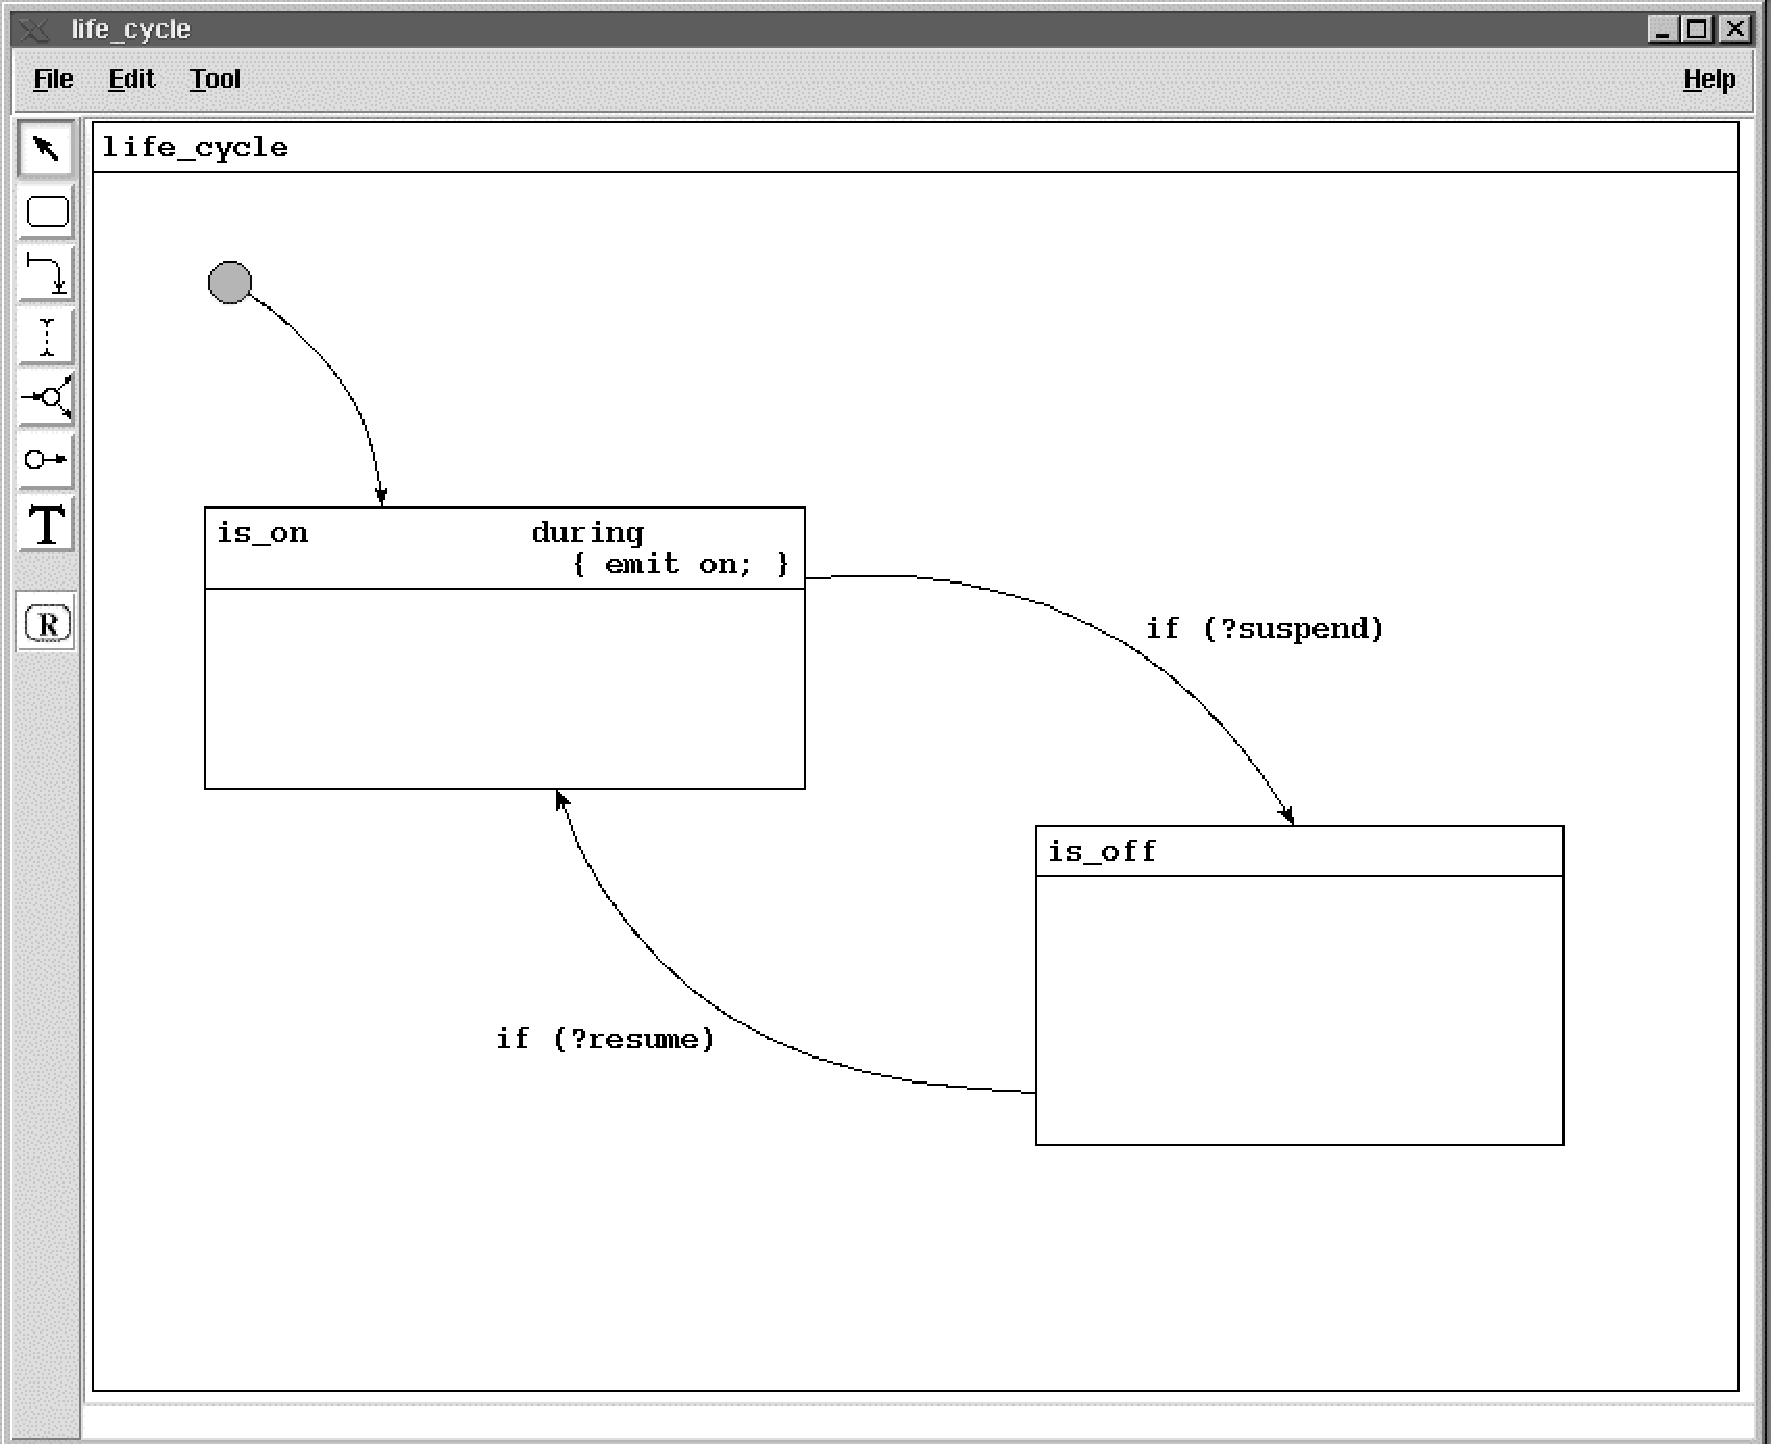
\epsfig{file=rctsty.epsf,width=300pt}
% \end{center}
% 
% 
% \paragraph{Blackboard implementation.} Blackboards are programmed in C and
% have to be started before any synchronous process may register.  In
% the present implementation, blackboards are based on the TCP/IP
% protocol.
% 
% If a synchronous process is created it automatically registers with
% blackboards (and automatically de-registers if terminated). Several
% synchronous processes may register at the same blackboard.
% 
% The protocol is thus: emittance of a network signal is transmitted to
% the blackboard at the end of an instant.  The blackboard uses the
% \pp{select then} operation to choose a value if several transmissions
% happen ``at the same time''.  The blackboard transmits the latched
% value to all registered synchronous process.  At each instant, a
% synchronous process polls for the network signals, and applies a memory copy
% to latch the value internally providing it with a time stamp. There
% may be several memory copies if the blackboard is related to several
% input signals.
% 
% This protocol is non blocking in that transmission, polling, and
% memory copy ask for a very small amount of time only (which
% nevertheless has to be considered if minimal cycle times for a
% synchronous process are computed).


%\chapter{Case Studies}\label{case-studies}

\emph{\ldots To be written \ldots}

%\section{A Transponder Lock}

%\section{DCF}

%\ldots



\begin{thebibliography}{9}

\bibitem{synccharts} C.~Andr\'e. Representation and analysis of
reactive behaviours: A synchronous approach, in: \emph{Proc. CESA'96},
Lille, France, July 1996.

\bibitem{berry} G.~Berry, The foundations of Esterel, in: G.~Plotkin,
C.~Stirling, and M.~Tofte (Eds.), \emph{Proofs, Languages, and
Interaction: Essays in Honour of Robin Milner}, MIT Press, 2000

\bibitem{constructivesemantics} G.~Berry, The Constructive Semantics
of Pure Esterel, Draft book,
\texttt{http://www-sop.inria.fr/meije/esterel/doc/main-papers.html}, 1999

\bibitem{esterel} G.~Berry and G.~Gonthier.  The \textsc{Esterel}
synchronous programming language: design, semantics, implementation.
{\em Science of Computer Programming}, 19(2):87--152, 1992.

\bibitem{synERJY} R.~Budde, A.~Poign\'e, K.-H-~Sylla.
synERJY - an Object-oriented Synchronous Language -.
Workshop on Synchronous Languages and Applications, Barcelona, 2004,\\
also: \emph{Electronic Notes in Theoretical Computer Science}, Volume 153

\bibitem{budde} R.~Budde, K.-H.~Sylla. 
Objektorientierte Echtzeit-Anwendungen auf Grundlage perfekter Synchronisation 
In: \emph{OBJEKTspektrum} 0(2):54-60, 1995, Zeitschrift f�r objektorientierte Technologien, M�nchen und 
SIGS Conferences GmbH M�nchen, Bd.Nr.7, 1995. 

\bibitem{budde2} R.~Budde, K.-H.~Sylla. 
ObjektorientiertBudde, R.; Merceron, A.; Sylla, K.H. 
Formal Verification as a Design Tool - The Transponder Lock Example 
In: Safe Comp'96, Vienna, Austria 23-25 October 1996, Proceedings of the 15th International Conference on Computer Safety, Reliability and Security, Springer Verlag, ISBN 3-540-76070-9 pp. 73-82. 

\bibitem{budde3} R.~Budde, A.~Poign\'e. 
Complex Reactive Control with Simple Synchronous Models 
ACM SIGPLAN  Workshop on Languages, Compilers, and Tools for Embedded Systems ( LCTES'00), Vancouver, Canada, June 2000, Lecture Notes in Computer Science 1985,
Springer, 2000

\bibitem{budde4} R.~Budde, P.~Pl``�o''ger, K.-H.~Sylla. 
A Synchronous Object-Oriented design flow for Embedded Applications 
In: Proc. \emph{2nd International Forum on Design Languages} (FDL), ECSI Verlag, Gi�res, 1999 

\bibitem{budde5} R.~Budde, M.~Pinna, A.~Poign\'e 
Coordination of Synchronous Programs 
In: P. Ciancarini, A.I. Wolf (eds.), \emph{3rd Int. Conf. on Coordination Languages and Models}, LNCS 1594, Springer, Heidelberg, 1999 

\bibitem{budde6} R.~Budde, A.~Poign\'e. 
On the synthesis of Distributed Synchronous Processes.
in: F.Cassez, C.Jard, B.Rozoy, M.Ryan (Eds.)
Proceedings of the summer School ``Modelling and Verification of Parallel
Processes'' (MOVEP'2k), Nantes, June 2000

\bibitem{Clarke} E.M.~Clarke, E.A.~Emerson, A.P.~Sistla, Automatic verification of finite-state concurrent systems using temporal logical specifications, in: \emph{ACM Transaction on Programming Languages and Systems}, 8(2):244-263,
1986

\bibitem{caspi} P.~Caspi, C.~Mazuet, R.~Salem, D.~Weber, Formal Design
of Distributed control Systems with Lustre, in: Proc.  Safecomp'99,
1999

\bibitem {java} J.~Gosling, B.~Joy, G.~Steele.\emph{The \java\
Language Specification}, Addison-Wesley, Nov. 1999

\bibitem{signal}  P.~Le Guernic, A.~Benveniste, P.~Bournaii, T.~Gautier,
Signal: a data-flow oriented language for signal processing, {\em
IEEE-ASSP}, 34(2), 1986.

\bibitem{halbwachs} N.~Halbwachs.  {\em Synchronous Programming of
Reactive Systems}, Kluwer Academic Publishers, Dordrecht, 1993.

\bibitem{observer} N.~Halbwachs, E.~Lagnier, and P.~Raymond. Synchronous 
observers and the verification of reactive systems. In: Third 
Int. Conference on Algebraic Methodology and Software Technology, AMAST�93, Workshops in Computing. Springer Verlag, 
June 1993. 

\bibitem{statecharts} D.~Harel. Statecharts: A visual approach to
complex systems, \emph{Science of Computer Programming}, 8:231--274, 1987.

\bibitem{lustre} N.~Halbwachs, P.~Caspi, P.~Raymond, and D.~Pilaud.
The synchronous dataflow programming language Lustre.
{\em Proceedings of the IEEE}, 79(9):1305--1320, 1991.

\bibitem{hol1} L.~Holenderski. 
LUSTRE - a verified production cell controller 
In: \emph{Formal development of reactive systems} / Lewerentz, Claus (Ed.), 101-112, 1995. NuSMV

\bibitem{hol2} L.~Holenderski, A.~Poign\'e. 
Synchronous Automata for Synchronous Programming Languages 
In: Wolisz, A. (Hrsg.); Schieferdecker, I. (Hrsg.); Rennoch, A. (Hrsg.), \emph{Formale Beschreibungstechniken f�r verteilte Systeme GI/ITG-Fachgespr�ch}, 19.-20. Juni 1997, Berlin, (GMD-Studien Nr. 315). Sankt Augustin: GMD, 1997, S. 129-134. ISBN 3-88457-315-2 
Full Paper in Postscript


\bibitem {rug-warrior} J.L.~Jones, A.M.~Flynn, {\em Mobile Robots - Inspiration to Implementation}, Wellesley,1993

\bibitem{kowalewski} S.~Kowalewski. Modellierungsmethoden aus der 
Informatik, at-Automatisierungstechnik, Heft
5(50): A1-A5, September 2001.

\bibitem{maffeis} O.~Maffeis, A.~Poign\'e. 
Synchronous Automata for Reactive, Real-Time or Embedded Systems 
(Arbeitspapiere der GMD Nr. 967). 
Sankt Augustin: GMD,  Schlo� Birlinghoven, D-53754 Sankt Augustin, ISSN 0723-0508, 51 S., 1996. 

\bibitem{Maranchini} F.~Maranchini, Y~.R\'emond.  Mode-Automata:
About Modes and States in Reactive Systems, Proc. European Symposium
on Programming, Lisbon, Portugal, 1998

\bibitem{argos} F.~Maranchini.  Operational and compositional
semantics of synchronous automaton compositions, In {\em Proceedings
of CONCUR'92}, volume 630 of {\em Lecture Notes in Computer Science},
Springer-Verlag, 550--564, Aug.  1992.

\bibitem{merceron} A.~Merceron, M.~M\"{u}llerburg, M.~Pinna. 
Verifying a time-triggered protocol in a multi-language environment 
In: Ehrenberger, W. (Hrsg.): \emph{Computer Safety, Reliability and Security}. Proc. 17th Intern. Conf. SAFECOMP'98. Lecture Notes in Computer Science (LNCS) No. 1516. 1998. pp 185-195. 

\bibitem{mue1} M.~M\"ullerburg. 
Systematic Testing: a Means for Validating Reactive Systems 
In: \emph{Software Testing}, Verification and Reliability 5(3):163-179 (1995). 
Selected papers from EuroSTAR'94 

\bibitem{mue2} M.~M\"ullerburg, L.~Holenderski, O.~Maffeis, A.~Merceron, M.~Morley. 
Systematic Testing and Formal Verification to Validate Reactive Programs 
In: \emph{Software Quality Journal} 4(4):287-307 (1995) 

\bibitem{mue3} M.~M\"{u}llerburg, R.~Budde. 
Validation und Verifikation in Synchronie: synchronousEifel 
In: GMA-Kongress '98 Mess- und Automatisierungstechnik. VDI-Berichte 1397, S. 299-308. D�sseldorf : VDI Verlag GmbH, 1998. 

\bibitem{NuSMV} The NUSMV website, \texttt{http://nusmv.irst.itc.it/}

\bibitem{systems} L.~Padulo, and M.~Arbib.  {\em System Theory - A Unified State-Space Approach to Continuous and Discrete Time Systems},
W.B.~Saunders Company, Philadelphia - London - Toronto, 1974.

\bibitem{Huth} C.S,~P�s�reanu, M.B.~Dwyer, M.~Huth. 
Assume-Gurantee Model-Checking of Software: A Comparative Case study.
\emph{Theoretical and Practical Aspects of SPIN Model Checking},Springer, 1999. 

\bibitem{PoHo} A.~Poign\'e, L.~Holenderski. 
\emph{Boolean Automata for Implementing Pure Esterel} 
Sankt Augustin: GMD, 1995, 47 S. (Arbeitspapiere der GMD Nr. 964). 

\bibitem {swb} A.~Poign\'e, M.~Morley, O.~Maffeis, L.~Holenderski, R.~Budde. 
The Synchronous Approach to Designing Reactive Systems 
In: \emph{Formal Methods in System Design}, 12, pp. 163-187 (1998), Kluwer Academic Publishers, The Netherlands.
 
\bibitem {multi} A.~Poign\'e, L.~Holenderski. 
The Multi-Paradigm Synchronous Programming Language LEA 
In Proceedings of the Int. Workshop on Formal Techniques for Hardware and Hardware-like Systems, 1998. 

\bibitem {combination} A.~Poign\'e, L.~Holenderski. 
On the Combination of Synchronous Languages 
In: W.P.de Roever (Hrsg.): Workshop on Compositionality: The Significant Difference, Malente September 8-12, 1997, LNCS 1536 Springer Verlag, pp. 490-514, 1998 

\bibitem {swb2} A.~Poign\'e, L.~Holenderski. 
Synchronie Workbench 
TOOLS 98, Y. Lakhnech, R. Berghammer (Hrsg.) Advances in Computer Science, 1999. 

\bibitem{reference} \se\ Reference Manual

\bibitem{userguide} \se\ Programming Environment User Guide


% \bibitem{Synccharts}
% C.~Andr\'e,
% \newblock Representation and Analysis of Reactive Behaviors: A Synchronous Approach,
% \newblock CESA'96, IEEE-SMC, Lille(F), 1996,
% 
% \bibitem{banatyne}
% R.~Bannatyne,
% \newblock Time Triggered Protocol: TTP/C,
% \newblock \emph{Embedded systems Programming}, 9/98, 52-54
% 
% \bibitem{benveniste}
% A.~Benveniste, B.~Cailland, and P.~leGuernic,
% \newblock From Synchrony to Asynchrony,
% \newblock In: J.C.M Baeten, and S. Mauw (eds.), CONCUR'99, LNCS 1664, 
% Springer, 1999
% 
% \bibitem{fhdl}
% R.~Budde, P.~Ploeger, K.H.~Sylla,
% \newblock A Synchronous object-oriented design Flow for Synchronous 
% Applications,
% \newblock Proc. FDL'99, ECSI Verlag, Gieres, 1999
% Springer, 1999
% 
% \bibitem{caspi}
% P.~Caspi, C.~Mazuet, R.~Salem, D.~Weber,
% \newblock Formal Design of Distributed control Systems with lustre,
% \newblock in: Proc. Safecomp'99, 1999
% 
% \bibitem{Esterel}
% G.~Berry and G.~Gonthier,
% \newblock The synchronous programming language Esterel: design, 
% semantics, implementation,
% \newblock {\em Science of Computer Programming}, 19:87--152, 1992.
% 
% \bibitem{Lustre}
% N.~Halbwachs, P.~Caspi, P.~Raymond, and D.~Pilaud,
% \newblock The synchronous data flow programming language Lustre,
% \newblock {\em Proceedings of the IEEE}, 79(9):1305--1321, Sep. 1991.
% 
% \bibitem{basement}
% H.~Hansson, H.~Lawson, O.~Bridal, S.~Larsson, H.~L\"{o}n, 
% M.~Str\"{o}mberg,
% \newblock BASEMENT: An Architecture and Methodology for Distributed 
% Automotive Real-Time Systems,
% \newblock {\em IEEE Transactions on Computers}, 48(9):1016--1027, Sep. 
% 1997.
% 
% 
% \bibitem{Statecharts} 
% D.~Harel,
% \newblock  STATECHARTS: A Visual Formalism for Complex Systems, 
% \newblock \emph{Science of Computer Programming}, 8(3)231-274,1987
% 
% \bibitem{Laprie} 
% J.C.~Laprie (Ed.),
% \newblock  \emph{Dependability: Basic Concepts and Terminology - in 
% English, French, German and Japanese}, 
% \newblock Vienna, Springer, 1992
% 
% 
% \bibitem{Signal} 
% P.~Le Guernic, T.~Gautier,M.~ Le Borgne,C.~ Le Maire,
% \newblock Programming Real-time Applications with SIGNAL, 
% \newblock \emph{Proceedings of  the IEEE}, 79(9), Sept. 1991
% 
% \bibitem{kopetz}
% H.~Kopetz,
% \newblock \emph{Real-Time systems: Design principles for distributed 
% Embedded applications},
% \newblock Kluwer Academic Publishers, 1997
% 
% \bibitem{combination}
% A.~Poign\'e, and L.~Holenderski, \newblock On the Combination of
% Synchronous Languages, \newblock In: W.P. de Roever (ed.),
% \emph{Workshop on Compositionality, The Significant difference}, LNCS
% 1536, Springer, Heidelberg, pp.  490 - 514, 1998.

\end{thebibliography}

\appendix

\newpage
\chapter{}\label{genesis}

\section{The genesis of synERJY: a personal recollection}\label{genesis}

The seed of what was to become \se\ was set when Gerard Berry and myself had 
a drink at a bar in San Gimignano somewhat about 1990. At his usual self, Gerard enthused about a new programming paradigm ``synchronous programming'', and his new programming language - \esterel.

This seed germinated when the then Embedded System Group at the then GMD
was looking for new themes in 1993 and Michele Pinna and myself
started to experiment with \esterel\ and more or less immediately
got convinced that synchronous programming may should have a future.

For whatever reason Michele and Leslek Holenderski started to think of
a new semantics for \esterel, probably they disliked the hardware semantics
of \esterel\ \cite{berry}. This was a trigger for myself, and some weeks
later on a spare afternoon I came up with the idea to use a hardware 
description like Berry but based on the assumption that every statement
should yield a sequential circuit which is started if a system signal $\alpha$
is present and that issues a system signal $\omega$ when it terminates.
Using this, I sat down and computed roughly 50 examples by hand, and got convinced that the approach was wothwile. Some other ``system variables''
emerged naturally, and I think it was Leslek who introduced a system variable
$\tau$ for preemption.

Then Leslek wrote a compiler for pure \esterel\ within weeks in Ocaml (which still is the implementation language of \se). The compiler turned
to be sound with regard to the original semantics.
 On the way, I found a very simple splitting
technique to deal with the reincarnation problem. Thia approach was
first presented at the C$^2$A autumn meeting in Paris in 1993.
A formal account has then been given in \cite{PoHo}
%, of which Klaus 
%Schneider claims it to be one the first complete proofs of correctness
% of a translation scheme of \esterel\ (\cite{Schneider})
 .

This was the starting point of many - sometimes competing - activities,
in which Reinhard Budde, Leslek Holenderski, Agathe Merceron, Olivier Maffeis, 
Matthew Morley, Monika M\"ullergburg, Michele Pinna, Axel Poign\'e,
and Karl-Heinz Sylla took part. Everybody intensively contributed
to the heated discussions, and it is difficult to give appropriate
credits to everybody in retrospect.

In these discussions, we tried to improve and optimise the translation
scheme. For instance, Matthew Morley and myself developed, and Matthew implemented another translation scheme in SML. In retrospect however, whatever came up did not really improve the translation scheme, and it is still - with minor changes - the basis of \se.

Almost immediately, the idea arose to extend the translation scheme to
the other synchronous formalisms as \argos\ and \lustre. This integration
was (almost) achieved with the \emph{Synchrony Workbench} \cite{swb}, that 
included a sophisticated front-end for \argos, also written by Leslek. Unfortunately, the approach had a semantic shortcoming, 
which was not so easy to fix, in particular since Leslek left the then GMD.
Nevertheless, the \se\ inherited much of the simulator of the Synchrony
Workbench then written by myself.

Based on the same translation scheme, Reinhard and Karl-Heinz
developed a combination of synchronous programming with objected-oriented
design starting in 1994. The object-oriented part was strongly influenced
by Eiffel, hence the language was called \emph{synchronousEifel} (Eifel being
a reference to the Eifel mountains close to Sankt Augustin), or \emph{sE} for 
short (still syntactically contained \se) \cite{budde}.

All this lead to a vision of a smooth integration of all synchronous
formalisms which has finally being stated in \cite{swb}. The vision then was 
even bolder, by far exceeding the given means; formal verification was tackled
as well testing and the problem dtribution. Agathe, Reinhard,
and Matthew worked on formal verification, Monika on testing, and Olivier on
distribution, and but everybody contributed to all subjects. 
This resulted in several publications (\cite{budde2}, \cite{budde3}, \cite{budde4}, \cite{hol1}, \cite{hol2}, \cite{maffeis}, \cite{merceron}, \cite{mue1}, \cite{mue2}, \cite{mue3}, \cite{multi}, \cite{combination}, \cite{swb2})
 but did not evolve into
a programming and verification environment as originally envisaged.

To make our efforts visible, we joined the EUREKA project SYNCRON, and 
subsequently became partners in the ESPRIT projects SYRF and\\ CRISYS. Further,
in order to propagate the gospel, Willem-Paul de Roever and myself discussed
the possibility of having a workshop for synchronous programming when he
visited GMD in Spring 94. This started the SYNCHRON workshop series, which
first took place in Dagstuhl in 1994.  Next it was important to get industry
interested, in particular in Germany. Hence Albert Benveniste and myself started
the series of the FEMSYS workshops, which was successfully staged in Munich in 1997, 1999, and 2001.

The ESPRIT project SYRF (``Synchronous Reactive Formalisms'') boosted the 
development of \se\ in that Reinhard, Karl-Heinz, and myself joined forces
to integrate and redevelop the different branches of development. Reinhard was
in charge of the object-oriented data part, and he wrote the lexer, parser
and typechecker as well as the code generator to C. Further he developed a new graphical editor for \se charts. Karl-Heinz programmed the control for the simulator, and took care of the backend compilers to diverse micro controllers, while myself focussed on the translation scheme of reactive part of the 
compiler, and on the gui aspects of the simulator and the programming environment.

In CRISYS (``CRitical Instrumentation and control SYStem'') we extended \se\ to support distribution using a blackboard like architecture (\cite{budde5}, 
\cite{budde6}), but this extension has remained experimental up to today. 

Development of the language itself had many interations always aiming for simplifying the concepts and for improving usability.
 A major change was the shift
to Java, or rather Java-like language) for the object-oriented data language, 
which was accomplished by Reinhard by implementing more or less a compiler
from Java to C. Motivation was not to deter users by a combination of two
relatively unknown languages, but to built on top of a fairly widely known
language such as Jave. Since then \se\ is a syntacically stable language though
minor changes at the fringes may still happen. A general overview over the
present language is to be found in \cite{synERJY}.
 
Within the Fraunhofer internal project FASPAS on adaptronics bwe have extended
the language by components dealing with vectors and arrays so that it becomes simple to program typical signal processing applications such as, e.g., filters.
Further, \se\ has been linked to MATLAB and scicos to support model-based design, and new backends for TI DSPs and Xilinx FPGAs have been added. Shakil
Ahmed linked \se\ to TI's DSP family and Motorola's MPC555. Further we developed
a proprietary DSP board based on TI's TMS329c6713 with four analogue inputs and four analogue outputs with AD/DA converters and anti-aliasing filters, and with
\se\ as input language.






\ \newline
Axel Poign\'e


%\chapter{Semantics}\label{semantics}

\paragraph{The general layout.}

Our intention is to provide a (slightly simplified) version of the
translation scheme for \se. The following schema explains the general
setting

\se\ programs are translated to an internal representation of the 
reactive part with a control structure in terms of a sequential
circuit and data part for the Java-like host language. Semantical
checks for causality and time races are performed on this internal
representation. Code for the different targets is generated from the
internal representation. The target code is typically C to which
back-end compilers are applied. For specific targets such as the
simulator, Simulink, or Scicos the C code is instrumented, but in a way
that the code kernel is exactly the one that runs on micro controllers,
DSPs, or similar like. The situation is special for verification and
FPGA generation. These translation demand for particular code formats
such as Verilog. However, in both cases the translations of the internal
code to these targets is of so elementary nature that we claim equivalence
of the resulting target code. This may be proved by code inspection comparing
the C code (which is annotated by readable version of the internal representation) with the other respective targets.

Thus we will only be concerned with the translation of the \se\ code
to the internal representation only.

\paragraph{A hardware translation.}

We define synchronous behaviour in terms of ``Synchronous Automata''
which have commands of the form
\begin{quote} 
\BEP
s <= $\phi$;          \textit{(Emittance of the signal \emph{s})}
r <- $\phi$;          \textit{(Setting a register \emph{r}} 
if ($s$)  $\!$\{ f \};    \textit{(triggering a data operation \emph{f})}
\EEP
\end{quote}
where $\phi$ is a Boolean expression respectively. The difference between
signals and registers is thus:
\begin{itemize}
\item the status of a signal can be read only in the instant it is emitted
\item the status of a register can be read only in the next instant after it has been set.
\end{itemize}
The difference is indicated by using the different symbols \pp{<=} and
\pp{<-}. The data operation \pp{f} is executed if the signal \pp{s} is present.

A \emph{synchronous automaton} consists of a sequence of such commands. The 
execution model is simple: the whole sequence of commands is executed exactly 
once at every instant. We refrain from spelling out a formal definition
of behaviour or semantics at this point, but believe that everybody will
have an intuitive understanding of how synchronous automata execute.

The translation scheme is compositional. Each statement generates a synchronous automaton, and the language operators of \se\ define operators on these automata.\footnote{Actually, one should be careful with the term compositionality here. The translation scheme is compositional but not the behaviour. The causality analysis will reschedule the sequence of equations genersted.} If there is any substantial idea in the translation scheme it the use of particular \emph{system signals} that are used in this translation scheme to glue together automata.

To give an example, we translate the elementary statement
\begin{center}
\pp{emit s}
\end{center}
The corresponding synchronous automaton is
\begin{quote} 
\BEP
 s <= $\alpha$;
 $\omega$ <= $\alpha$;
 $\kappa$ <= false;
\EEP
\end{quote}
Here $\alpha$ is the \emph{start} signal, and $\omega$ the termination. Execution of the automaton starts if $\alpha$ is present, and terminates
at the same instant. Then $|omega$ will be present at the same instant.
The signal $\kappa$ stands for ``is in control'', meaning that the automaton
does not terminate at the given instant. of course, the emit statement
never gets control.

Somewhat more elaborated is the translation of \pp{await ?s}:
\begin{quote} 
\BEP
    r <- !s \& ($\alpha$ | r);
    $\omega$ <=  s \& ($\alpha$ | r);
    $\kappa$ <= r;
\EEP
\end{quote}
Here a new \emph{control register} \pp{r} is generated. The automaton keeps
control until the signal \pp{s} is present. It then terminates at the same
instant, and looses control.

\emph{Sequential composition} now almost comes for free. Assume that $A_{1}$ and $A_{2}$ are synchronous automata. Then ``$A_{1}\ A_{2}$'' denotes the synchronous automaton
\begin{quote} 
\BEP
 $A_{1}[\gamma/\omega,\kappa_{1}/\kappa]$
 $A_{2}[\gamma/\alpha,\kappa_{2}/\kappa]$
 $\kappa$ <= $\kappa_{1}$ | $\kappa_{2}$;
\EEP
\end{quote}
where $\gamma$, $\kappa_{1}$, $\kappa_{2}$ are new pure signals ($\gamma/\omega$ denotes the substitution of $\omega$ by $\gamma$). If started $A_{1}$ is executed. If $A_{1}$ terminates, $A_{2}$ is started. The sequential composition is in control if one of the sub-automata is in control.

We apply these rules to
\begin{quote}
\BEP
    emit car\_to\_red;
    await ?car\_red;
\EEP
\end{quote}
and obtain the synchronous automaton
\begin{quote}
\BEP
car\_to\_red <= $\alpha$;
       $\gamma$  <= $\alpha$;
       $\kappa_{1}$ <= false;
       r  <- !car\_red \& ($\gamma$ or r);
       $\omega$  <= car\_red  \& ($\gamma$ or r);
       $\kappa_{2}$ <= r;
       $\kappa$  <= $\kappa_{1}$ | $\kappa_{2}$;    
\EEP
\end{quote}

The \emph{parallel composition} ``\pp{$A_{1}$ || $A_{2}$;}'' is slightly more complicated. If started, both the sub-automata start to execute. The parallel composition
terminates if either both sub-automata terminate at the same instant, of if
one of the sub-automata terminates while the other has terminated computation at an earlier instant. Here the control signal $\kappa$ comes handy:
\begin{quote}
\BEP
    $A_{1}$[$\omega_{1}$/$\omega$,$\kappa_1$/$\kappa$]
    $A_{2}$[$\omega_{2}$/$\omega$,$\kappa_2$/$\kappa$]
    $\omega$ <=    $\!\omega_1$ \& $\omega_2$ 
         | $\omega_1$ \& $\kappa_1$ \& not $\kappa_2$ 
         | $\omega_2$ \& $\kappa_2$ \&  !$\kappa_1$;
    $\kappa$ <= $\kappa_1$ or $\kappa_2$;
\EEP
\end{quote}
The condition  ``\pp{$\omega_1$ \& $\kappa_1$ \& !$\kappa_2$}''
states: if the automaton $A_{1}$ is in control and terminates, and
if the automaton $A_{2}$ is not in control (has terminated earlier),
then the parallel composition terminates. 

The \emph{loop statement} ``\pp{loop \{ $A$ \};}'' is again simple
\begin{quote}
\BEP
   $\gamma$ <= $\alpha$ \& $\omega_{1}$;
   $A$[$\gamma$/$\alpha$,$\omega_{1}$/$\omega$]
   $\omega$ <= false;
\EEP
\end{quote}
as is the \emph{conditional} ``\pp{if ($\phi$) \{ $A_{1}$ \} else \{ $A_{2}$ \}}''
\begin{quote}
\BEP
   $\gamma_{1}$ <= $\phi$ \& $\alpha$;
   $\gamma_{2}$ <= not $\gamma_{1}$ \& $\alpha$;
   $A_{1}$[$\gamma_{1}$/$\alpha$,$\omega_{1}$/$\omega$,$\kappa_{1}$/$\kappa$]
   $A_{2}$[$\gamma_{2}$/$\alpha$,$\omega_{2}$/$\omega$,$\kappa_{2}$/$\kappa$]
   $\omega$ <= $\omega_{1}$ | $\omega_{2}$;
   $\kappa$ <= $\kappa_{1}$ | $\kappa_{2}$;
\EEP
\end{quote}
with \pp{r} being a new control register. Note that $A$ should always be in control for the loop statement because otherwise $A$ would be executed infinitely often at one instant. The conditional can easily be iterated.

The power of the imperative part of the language stems from the \emph{pre-emption statement}. In preparation, we take a closer look at the \pp{halt} statement. It keeps control forever except if it pre-empted. We model pre-emption by introducing a new system signal $\tau$ which is supposed to trigger pre-emption. For each \pp{halt} statement a control register $r$ is generated

\begin{quote}
\BEP
    $r$ <- $\alpha$ | !$\tau$ \& r;
    $\omega$ <= $\tau$ \& r;
    $\kappa$ <= r;

\EEP
\end{quote}
Pre-emption is then modelled using the system signal $\tau$. We consider a simple case of the cancel statement
\begin{quote}
\BEP
    cancel \{
       $A$
    \} when ($\phi_{1}$) \{ $A_{1}$ \}
       \ldots
       else when ($\phi_{n}$) \{ $A_{n}$ \}    
\EEP
\end{quote}
that translates to
\begin{quote}
\BEP
    $\tau_{1}$ <= $\tau$ | $\kappa$ \& ($\phi_{1}$ | \ldots | $\phi_{n}$);
    $A$[$\tau_{1}$/$\tau$]
    $\gamma_{1}$ <= $\tau_{1}$ \& $\phi_{1}$;
    $A_{1}$[$\gamma_{1}$/$\alpha$,$\kappa_{1}$/$\kappa$]
    \ldots
    $A_{1}$[$\gamma_{1}$/$\alpha$,$\kappa_{1}$/$\kappa$]
\EEP
\end{quote}
The automaton $A$ is pre-empted if it is in control, and if one of the conditions $\phi_{i}$ becomes true. Then the respective branch is executed. The other cases like strong pre-emption are considerably more complicated and omitted here. Note that the cancel statement may be pre-empted from the context, hence the \pp{$\tau$ | \ldots}.

Just to convince ourselves that the translation scheme operates properly, let us consider the statement
\begin{quote}
\BEP
     await ($\phi$); = cancel \{
                       loop \{
                          next;
                       \};
                   \} when ?s;
\EEP
\end{quote}
The next statement is defined by 
\pp{next;} statement
\begin{quote}
\BEP
    r <- $\alpha$; 
    $\omega$ <= $\tau$ \& r;
    $\kappa$ <= !$\tau$ \& r;
\EEP
\end{quote}
Not surprisingly, the loop generates
\begin{quote}
\BEP
    $r$ <- $\alpha$ | $\gamma$;
    $\gamma$ <= $\tau$ \& r;
    $\kappa$ <= !$\tau$ \& r;
    $\omega$ <= false;
\EEP
\end{quote}
which exactly is the semantics of the halt statement. The cancel statement then generates (modulo renaming and rearrangement, and using that $A_{1}$ is the nothing statement)
\begin{quote}
\BEP
    $\tau_{1}$ <= $\tau$ | $\kappa$ \& ?$s$;
    $r$ <- $\alpha$ | $\gamma$;
    $\gamma$ <= $\tau$ \& r;
    $\kappa$ <= !$\tau$ \& r;
    $\omega$ <= false;
     $\omega$ <= $\tau$ \& r;
    $\omega$ <= $\tau$ \& ?$s$;
\EEP
\end{quote}
This is equivalent to 
\begin{quote} 
\BEP
    r <- !s \& ($\alpha$ | r);
    $\omega$ <=  s \& ($\alpha$ | r);
    $\kappa$ <= r;
\EEP
\end{quote}


and 
We omit translation of the other available constructs to the reader who also
may want to check that the \emph{await} statement does not need its own translation rule but can be synthesised 

\paragraph{Dealing with data.}

Using \pp{await x > 5} we demonstrate the interaction of data and control
The obvious idea is that if started a time counter is set to 0 that is
increased by the ddelta of time \pp{dt} at every instant till the counter exceeds the time limit of 30 seconds.
l\"{a}sst sich die Interaktion von
\begin{quote}
\BEP
    r <- $\alpha$ | !$\delta$ \& r; 
    if (r) \{ $\delta$ = x > 5 \};
    $\omega$ <= $\delta$ \& r;
    $\kappa$ <= r;
\EEP
\end{quote}
The counter is initialized when \pp{alpha} is present.
The other data actions are executed whenever the register \pp{r} is set. The register is set for the next instant when \pp{alpha} is present. The Boolean signal $\delta$ interfaces the data with the control structure.

The general idea is thus: data actions like routine calls, assignments, etc. 
are embedded by the scheme
\begin{quote}
\BEP
    if ($\alpha$) \{ \emph{data action} \};
    $\omega$ <= $\alpha$;
    $\kappa$ <= \emph{ff};
\EEP
\end{quote}
and atomic Boolean expressions by
\begin{quote}
\BEP
    if ($\alpha$) \{ $\delta$ = \emph{atomic proposition} \};
    $\omega$ <= $\alpha$;
    $\kappa$ <= \emph{ff};
\EEP
\end{quote}
One notices a clear separation of control and data operations that are activated by signals and that provide feedback using pure signals.

to be continued

%\paragraph{Reincarnation.}

%
%\paragraph{Translating \se charts.}
%\statecharts~\cite{statecharts}

%\paragraph{Finally, data flow.}

%\lustre~\cite{lustre} 

%\paragraph{On scheduling.}

%Der \"{U}berschrift ``Von Verhalten zu Schaltwerken'' enth\"{a}lt
%implizit die Behauptung, dass die \"{U}bersetzung (sequentielle)
%Schaltwerke erzeugt.  Damit dies der Fall ist, muss f\"{u}r synchrone
%Automaten zus\"{a}tzlich gelten, dass jedes Signal nur noch gelesen
%werden kann, wenn es einmal emittiert ist (``write-before-read'').

%Nun macht man sich leicht klar, dass der \"{U}bersetzungsprozess die 
%Eigenschaft nicht notwendig gew\"{a}hrleistet. Zum Beispiel erzeugt 
%das Programm
% 
%\begin{quote}
%\BEP
%    await (not ?a);
%    emit a;
%\EEP
%\end{quote}
% 
%den synchronen Automaten
% 
%\begin{quote}
%\BEP
%    r  <-      a  and ($\alpha$ or r);
%    $\gamma$  <= (not a) and ($\alpha$ or r);  //    (1)
%    $\kappa_{1}$ <= r;   
%    a  <= $\gamma$;                     //    (2)
%    $\omega$  <= $\gamma$;
%    $\kappa_{2}$ <= false;
%    $\kappa$  <= $\kappa_{1}$ or $\kappa_{2}$;
%\EEP
%\end{quote}

%Wenn wir annehmen, dass das Signal \pp{a} nicht pr\"{a}sent ist, wird
%das Warten beendet ($\gamma$ wird wahr  (1)), und \emph{das Signal
%\pp{a} emittiert} (2); es ist in einem Takt also absent und pr\"{a}sent,
%im Widerspruch zu den Annahmen des synchronen Auswertungsmodells.

%Ein anderes Beispiel ist
% 
%\begin{quote}
%\BEP
%    [[ await (not ?a);
%    || emit a;
%    ]];
%\EEP
%\end{quote}
% 
%das in den synchronen Automaten
% 
%\begin{quote}
%\BEP
%    r  <-      a  and ($\alpha$ or r);
%    $\omega_{1}$ <= (not a) and ($\alpha$ or r);
%    $\kappa_{1}$ <= r;   
%    a  <= $\alpha$;
%    $\omega_{2}$ <= $\alpha$;
%    $\kappa_{2}$ <= false;
%    $\omega$  <=    $\!\omega_1$ and $\omega_2$ 
%          or $\omega_1$ and $\kappa_1$ and not $\kappa_2$ 
%          or $\omega_2$ and $\kappa_2$ and not $\kappa_1$;
%    $\kappa$  <= r;
%\EEP
%\end{quote}

%\"{u}bersetzt. Scheinbar liegt ein ``read-before-write'' Konflikt vor.

%

%der aber durch einfaches Umsortieren der Befehle ohne 
%Bedeutungsver\"{a}nderung gel\"{o}st werden kann. Dies ist im 
%vorhergehenden Fall nicht m\"{o}glich.

%Generell muss der Kompilierer eine synchronen Sprache die
%\"{U}bersetzung durch ein statisches Scheduling erg\"{a}nzen, das
%``read-before-write'' Konflikte aufl\"{o}st, wenn es m\"{o}glich ist, 
%und Programme andernfalls zur\"{u}ckweist.

%
% Nun mag man sich nach den Vorteilen fragen, wenn erzwingt, dass 
% Signale nur vor einem Lesezugriff geschrieben werden k\"{o}nnen. 
% 
% 

% Alle Zyklen m\"{u}ssen \"{u}ber Register gehen.
% 
% Man beachte, dass sowohl der \"{U}bersetzungsmechanismus wie der 
% erzeugte (Zwischen-) Kode der synchronen Automaten elementar ist. Dies 
% erh\"{o}ht die Verl\"{a}sslichkeit des erzeugten Kodes zumindest in der 
% Hinsicht, dass der Kompilerer die Semantik pr\"{a}zise abbildet.

%\begin{thebibliography}{9}

%    \bibitem{sp1} R.~Budde, A.~Poign\'e, K.H.~Sylla. Synchrone 
%    Programmierung - Grundlagen, at-Automatisierungstechnik, Heft
%    4(50): A31-A34, April 2002

%    \bibitem{sp2} R.~Budde, A.~Poign\'e, K.H.~Sylla. Synchrone 
%    Programmierung - Sprachen, at-Automatisierungstechnik, Heft
%    7(50): A39-A42, Juli 2002.

%    \bibitem{sp3} R.~Budde, A.~Poign\'e, K.H.~Sylla. Synchrone 
%    Programmierung - Anwendung, at-Automatisierungstechnik, Heft
%    8(50): A39-A42, August 2002.

%    \bibitem{Clarke} J.R.~burch, E.M.~Clarke, K.L.~McMillan, D.L.~Dill, 
%    L.J.Hwang. symbolic Model checking: $10^{20}$ States an Beyond, 
%    \emph{Information and Computation}, 98(2):142-170,June 1992.
%    
%				\bibitem{SDL} J.~Ellsberger, D.~Hogrefe, A.~Sarma,\emph{SDL -
%				Formal Object-oriented Language for Communicating Systems}. 
%				Prentice Hall Europe, 1997, ISBN 0-13-621384-7.
%  
%    \bibitem{lustre} N.~Halbwachs, P.~Caspi, P.~Raymond, and
%				D.~Pilaud.  The synchronous dataflow programming language Lustre. 
%				{\em Proceedings of the IEEE}, 79(9):1305--1320, 1991.

%				\bibitem{statecharts} D.~Harel.  Statecharts: A visual approach to
%				complex systems, \emph{Science of Computer Programming},
%				8:231--274, 1987.
%    
%				\bibitem{se} \texttt{http://www.ais.fraunhofer.de/~ap/sE}

%\end{thebibliography}

%
% \begin{thebibliography}{}
%     
% \bibitem{Synccharts}
% C.~Andr\'e,
% \newblock Representation and Analysis of Reactive Behaviors: A Synchronous Approach,
% \newblock CESA'96, IEEE-SMC, Lille(F), 1996,
% 
% \bibitem{banatyne}
% R.~Bannatyne,
% \newblock Time Triggered Protocol: TTP/C,
% \newblock \emph{Embedded systems Programming}, 9/98, 52-54
% 
% \bibitem{benveniste}
% A.~Benveniste, B.~Cailland, and P.~leGuernic,
% \newblock From Synchrony to Asynchrony,
% \newblock In: J.C.M Baeten, and S. Mauw (eds.), CONCUR'99, LNCS 1664, 
% Springer, 1999
% 
% \bibitem{fhdl}
% R.~Budde, P.~Ploeger, K.H.~Sylla,
% \newblock A Synchronous object-oriented design Flow for Synchronous 
% Applications,
% \newblock Proc. FDL'99, ECSI Verlag, Gieres, 1999
% Springer, 1999
% 
% \bibitem{caspi}
% P.~Caspi, C.~Mazuet, R.~Salem, D.~Weber,
% \newblock Formal Design of Distributed control Systems with lustre,
% \newblock in: Proc. Safecomp'99, 1999
% 
% \bibitem{Esterel}
% G.~Berry and G.~Gonthier,
% \newblock The synchronous programming language Esterel: design, 
% semantics, implementation,
% \newblock {\em Science of Computer Programming}, 19:87--152, 1992.
% 
% \bibitem{Lustre}
% N.~Halbwachs, P.~Caspi, P.~Raymond, and D.~Pilaud,
% \newblock The synchronous data flow programming language Lustre,
% \newblock {\em Proceedings of the IEEE}, 79(9):1305--1321, Sep. 1991.
% 
% \bibitem{basement}
% H.~Hansson, H.~Lawson, O.~Bridal, S.~Larsson, H.~L\"{o}n, 
% M.~Str\"{o}mberg,
% \newblock BASEMENT: An Architecture and Methodology for Distributed 
% Automotive Real-Time Systems,
% \newblock {\em IEEE Transactions on Computers}, 48(9):1016--1027, Sep. 
% 1997.
% 
% 
% \bibitem{Statecharts} 
% D.~Harel,
% \newblock  STATECHARTS: A Visual Formalism for Complex Systems, 
% \newblock \emph{Science of Computer Programming}, 8(3)231-274,1987
% 
% \bibitem{Laprie} 
% J.C.~Laprie (Ed.),
% \newblock  \emph{Dependability: Basic Concepts and Terminology - in 
% English, French, German and Japanese}, 
% \newblock Vienna, Springer, 1992
% 
% 
% \bibitem{Signal} 
% P.~Le Guernic, T.~Gautier,M.~ Le Borgne,C.~ Le Maire,
% \newblock Programming Real-time Applications with SIGNAL, 
% \newblock \emph{Proceedings of  the IEEE}, 79(9), Sept. 1991
% 
% \bibitem{kopetz}
% H.~Kopetz,
% \newblock \emph{Real-Time systems: Design principles for distributed 
% Embedded applications},
% \newblock Kluwer Academic Publishers, 1997
% 
% \bibitem{combination}
% A.~Poign\'e, and L.~Holenderski, \newblock On the Combination of
% Synchronous Languages, \newblock In: W.P. de Roever (ed.),
% \emph{Workshop on Compositionality, The Significant difference}, LNCS
% 1536, Springer, Heidelberg, pp.  490 - 514, 1998.
% 
% 
% \end{thebibliography}

% 
% 
% 
% Wir definieren ein einfaches operationales Modell, \emph{synchrone
% Automaten}, und \"{u}bersetzen einige typische Sprachelemente der
% synchronen Programmierung in dieses Modell.
% 
% \subsection{Eine einfaches operationales Modell}\label{Modell}
% 
% Wir pr\"{a}sentieren das Verhalten eines synchronen Automaten $P$
% syntaktisch durch eine Sequenz von Befehlen $p$ der Form
% \begin{quote}
%     \begin{tabular}{ll}
%         $s \Leftarrow \phi$; & // das Signal $s$ wird emittiert \\
%         $c \leftarrow \phi$; & // das Kontrollregister $c$ \ldots\\
%                                 & // \ldots wird gesetzt  \\
%         $if\ (?a)\ \{\ action;\ \};$ & // konditionale Aktion\\
%         $s\Leftarrow cond;$ & // Boolesche Aktion
%     \end{tabular}
% \end{quote}
% Die Bedingung $\phi$ ist ein Boolescher Ausdruck.  Der atomare
% Boolesche Ausdruck $?a$ fragt, ob das Signal $a$ pr\"{a}sent'' ist.
% 
% Deren Bedeutung wird durch \emph{Mikroschritte} der Form  
% $$(\kappa',\sigma',E')  \ARROW{\kappa}{p}  (\kappa'',\sigma'',E'')$$ 
% definiert.  Dabei sind $E' \subseteq E''$ Mengen von \emph{Signalen},
% $\kappa$ und $\kappa' \subseteq \kappa''$ Mengen von
% \emph{Kontrollregistern} und $\sigma'$ und $\sigma''$
% \emph{Speicherzust\"{a}nde}.  Die Menge $\kappa$ bezeichnet den
% Kontrollzustand zu Beginn eines Taktes.  Die Menge der Signale, die
% emittiert werden, und die Menge der Kontrollzust\"{a}nde, die f\"{u}r
% den n\"{a}chsten Takt gesetzt werden akkumulieren.  Daher die
% Forderung, dass $E' \subseteq E''$ und $\kappa' \subseteq \kappa''$.
% 
% Im Einzelnen gelte, dass
% $$(\kappa',\sigma',E)  \ARROW{\kappa}{s\ \Leftarrow\ \phi;} 
% (\kappa',\sigma',E\cup\{s\})$$ 
% 
% $$(\kappa',\sigma',E)  \ARROW{\kappa}{c\ \leftarrow\ \phi;} 
% (\kappa'\cup\{c\},\sigma',E)$$
% 
% $$(\kappa',\sigma',E') \ARROW{\kappa}{if\ (?a)\ \{\ action;\ \};}
% (\kappa',action(\sigma'),E')$$
% 
% $$(\kappa',\sigma',E') \ARROW{\kappa}{s\ \Leftarrow\ cond;}
% (\kappa',\sigma',E'\cup\{s\})$$
% Dabei gelte, dass die Bedingung $\phi$, bzw.  $?a$, im Kontrollzustand
% $\kappa$ und dem Speicherzustand $\sigma'$ bei anliegenden Signalen
% $E'$ erf\"{u}llt ist.  Wir dr\"{u}cken dies mit der Notation
% $\kappa,\sigma',E' \models \phi$ aus, ohne die Definition
% auszuf\"{u}hren.  Entsprechend gelte f\"{u}r die letzte Regel, das die
% Datenbedingung \emph{cond} im Zustand $\sigma$ erf\"{u}llt und das
% Signal $s$ pr\"{a}sent ist.  Man beachte , dass der Kontrollzustand
% $\kappa$ durch einen Mikroschritt nicht ver\"{a}ndert wird.
% 
% Wir wollen die Wertzuweisung $s = e;$ auf ein Feld $x$ als eine
% spezielle Aktion einf\"{u}hren.  Es gelte, dass 
% $$(\kappa',\sigma',E)
% \ARROW{\kappa}{if\ (?a)\ \{\ x = e;\ \};}
% (\kappa',\sigma[s/v_{e}],E)$$ 
% Der Wert $v_{e}$ des Ausdruckes $e$ im aktuellen Kontext wird dem Feld
% $x$ zugewiesen, wenn die Bedingung $?a$ erf\"{u}llt ist.  Wir
% vereinbaren, dass zu jedem Signal $s$ ein Feld $\$s$ zugeh\"{o}rig
% ist.
% 
% Sei $P = p_{1} \ldots p_{n}$ ein synchroner Automat.  In jedem Takt
% f\"{u}hrt $P$ einen \emph{Makroschritt}
% $$(\kappa,\sigma)  \ARROW{E/E'}{P}  (\kappa',\sigma')$$
% aus.  Ein Makroschritt entsteht aus einer Folge von 
% Mikroschritten
% $$(\emptyset,\sigma,E \backslash E')
% \ARROW{\kappa}{p_{1}} (\kappa_{1},\sigma_{1},E_{1})
% \ARROW{\kappa}{p_{2}} \ldots
%  \ARROW{\kappa}{p_{n}} (\kappa',\sigma',E')$$ 
% Dabei ist $E$ die Menge aller Signale und $E'$ die Menge der von $P$
% emittierten Signale.  Ein Makroschritt ver\"{a}ndert den
% Kontrollzustand.  In den Mikroschritten werden die Kontrollregister
% akkumuliert, die f\"{u}r den n\"{a}chsten Makroschritt gesetzt wird.
%  
% Makroschritte unterliegen der Einschr\"{a}nkung, dass
% \begin{itemize}
%     \item \emph{ein Signal $s$ nur dann emittiert und dem
%     zugeh\"{o}rigen Feld $s$ nur dann ein Wert zugewiesen werden
%     darf, wenn zuvor weder dessen Pr\"{a}senz abgefragt noch dessen
%     Wert benutzt wurde}.
% \end{itemize}
% Wir bezeichnen diese Eigenschaft als \emph{Konsistenz}.  Sie
% gew\"{a}hrleistet, dass, wie im synchronen Auswertungsmodell
% gefordert, die Pr\"{a}senz und der Wert eines Signals w\"{a}hrend
% eines Taktes konsistent ist, d.h. jeder Zugriff auf Pr\"{a}senz oder
% Wert liefert das gleiche Ergebnis.  Alternativ l\"{a}sst sich von
% einer \emph{write-before-read} Strategie sprechen.
% 
% Man beachte das andere Daten in einem Takt durchaus mehrfach 
% ver\"{a}ndert werden k\"{o}nnen: Sei $x$ ein Feld. Dann bindet die 
% Sequenz 
% $$x = 0; x = x + 1;$$
% zun\"{a}chst den Wert $0$ an das Feld $x$ und dann den Wert $1$. 
% Dies bedingt die etwas komplexe Definition des Verhaltens.
% 
% \subsection{Kausalit\"{a}t}
% Nicht jeder synchrone Automat gen\"{u}gt der Konsistenz Bedingung, z.B.
% $$if\ (?s)\ \{ action; \};\ s\ \Leftarrow\ \phi$$
% Ein solches Programm wird als \emph{kausal inkorrekt} 
% zur\"{u}ckgewiesen. Ein weiteres Beispiel ist
% $$if\ (\$s == 5)\ \{\ action;\ \};\ \$s = 5$$
% 
% Signal- wie Datenfluss und deren Kombination definieren \emph{kausale}
% Beziehungen zwischen den Befehlen eines synchronen Automaten.  Wenn
% diese Beziehungen eine Halbordnung definieren, ist der Automat
% konsistent.  Bei der \"{U}bersetzung synchroner Sprachen \"{u}bernimmt
% der Kompiler die Analyse der \emph{Kausalit\"{a}t}.  Er garantiert die
% Konsistenz des erzeugten synchronen Automaten und damit auch
% offentsichtlich eine deterministische Auswertung (bei gegebenen
% Eingangssignalen).
% 
% Dass die kausalen Beziehungen nur eine Halbordnung definieren wird an 
% einem einfachen Beispiel deutlich:
% $$s\ \Leftarrow\ \phi;\ if\ (?s)\ \{ action; \};\ s'\ \Leftarrow\ \phi';\ if\ (?s')\ \{ action'; \}$$
% Es gelten die folgenden Ordnungsbeziehungen
% $$s\ \Leftarrow\ \phi;\quad < \quad if\ (?s)\ \{ action; \}$$
% $$s'\ \Leftarrow\ \phi';\quad < \quad if\ (?s')\ \{ action'; \}$$
% Diese ebenso f\"{u}r
% $$s\ \Leftarrow\ \phi;\ s'\ \Leftarrow\ \phi';\ if\ (?s)\ \{ action; \};\ if\ (?s')\ \{ action'; \}$$
% Es ist somit m\"{o}glich die Sequenz der Befehle eines synchronen 
% Automaten zu ver\"{a}ndern, ohne dessen Semantik zu ver\"{a}ndern.
% Die Bedeutung dieser Beobactung wird im n\"{a}chsten Abschnitt deutlich.
% 
% Es gilt nachzutragen, dass Kontrollregister den kausalen Fluss brechen. 
% Die Sequenz
% $$if\ (?c)\ \{ action; \};\ c\ \Leftarrow\ \phi$$
% ist konsistent, wenn $c$ ein Kontrollregister bezeichnet.  Die Abfrage
% $?c$, ob das Kontrollregister $c$ gesetzt ist, bezihe sich auf den
% Kontrollzustand zu Beginn des Makroschritts.  Der Befehl $c\
% \Leftarrow\ \phi$ setzt das Kontrollregister f\"{u}r den nachsten
% Makroschritt.
% 
% \subsection{Zur \"{U}bersetzung von synchroner Sprachstrukturen}
% Wir wollen als Invariante annehmen, dass jeder durch die \"{U}bersetzung 
% erzeugte Automat die folgenden sogenannten \emph{Systemsignale} liest oder schreibt:   
% \begin{itemize}
%     \item  ein \emph{Startsignal} $\alpha$,
% 
%     \item ein \emph{Terminationssignal} $\omega$,
% 
%     \item  ein \emph{Triggersignal} $\beta$,
% 
%     \item  ein \emph{Abbruchsignal} $\tau$ und
% 
%     \item  ein \emph{Kontrollsignal} $\kappa$.
% \end{itemize}
% Die Signale $\alpha$, $\beta$ und $\tau$ werden gelesen und die 
% Signale $\omega$ und $\kappa$ werden geschrieben. Deren Bedeutung 
% wird nachfolgend sukzessive erk\"{a}rt. 
% 
% 
%  
% Wir \"{u}bersetzen zun\"{a}chst die Sprachkonstrukte des reaktiven 
% Kerns in Befehlssequenzen eines synchronen Automaten. Die Notation 
% \pp{P[x/y]} bedeute, dass das Signal \pp{x} \"{u}berall in \pp{P} durch 
% das Signal \pp{y} ersetzt wird.  
% \begin{description}
%     \item[emit s:]\
% %     
%    \BEP
%        s $\Leftarrow$ $\alpha$;
% %        if (?$\alpha$) \{ \$s := e; \};
%        $\omega$ $\Leftarrow$ $\alpha$;
%        $\kappa$ $\Leftarrow$ false;
%    \EEP
% %     
%     Die Sequenz terminiert in demselben Takt, in dem
% sie gestartet wird (\pp{$\omega$ $\Leftarrow$ $\alpha$;}) und
% \"{u}bernimmt niemals die Kontrolle (\pp{$\kappa$ $\Leftarrow$
% false;}).
% 
%    \item[next:]\
% % 
%    \BEP
%       $\rho$ $\Leftarrow$ !$\tau$ \& $\alpha$;
%       $\kappa$ $\Leftarrow$ $\rho$
%       $\omega$ $\Leftarrow$ $\beta$ \& !$\rho$;
%     \EEP
% % 
%     Das Register $\rho$ wird bei Start gesetzt, wenn kein
%     Abbruchsignal anliegt.  Das Register beh\"{a}lt die Kontrolle, bis 
%     in einem der folgenden Takte das Triggersignal $\beta$ pr\"{a}sent 
%     ist. In diesem Falle terminiert die Sequenz.
% 
%    \item[P Q:]\
% % 
%    \BEP
%       P[$\omega$/$\gamma$,$\kappa$/$\kappa_1$]
%       Q[$\alpha$/$\gamma$,$\kappa$/$\kappa_2$]
%       $\kappa$ $\Leftarrow$ $\kappa_1$ | $\kappa_2$;      
%    \EEP
% %   
%    Zun\"{a}chst wird die Sequenz \pp{P} gestartet. Wenn diese 
%    terminiert, wird in demselben Takt die Sequenz \pp{Q} gestartet.
%    
%    \item[if c \{ P \} else \{ Q \}:]\
% % 
%    \BEP
%      $\delta$  $\Leftarrow$ $\alpha$ \& c;
%      $\alpha_1$ $\Leftarrow$ $\alpha$ \& $\delta$;
%      $\alpha_2$ $\Leftarrow$ $\alpha$ \& !$\alpha_1$;
%      P[$\alpha$/$\alpha_1$,$\omega$/$\omega_1$,$\kappa$/$\kappa_1$]
%      Q[$\alpha$/$\alpha_2$,$\omega$/$\omega_1$,$\kappa$/$\kappa_2$]
%      $\kappa$ $\Leftarrow$ $\kappa_1$ | $\kappa_2$; 
%      $\omega$ $\Leftarrow$ $\omega_1$ | $\omega_2$; 
%    \EEP
% %   
%    
% 
% 
%    \item[loop \{ P \}:]\
% % 
%    \BEP
%       $\gamma$ $\Leftarrow$ $\alpha$ | $\omega_1$;
%       P[$\alpha$/$\gamma$,$\omega$/$\omega_1$]
%       $\omega$ $\Leftarrow$ false;      
%    \EEP
% %   
% 
% 
%    \item[cancel \{ P \} when (c):]\
% % 
%    \BEP
%       $\delta$ $\Leftarrow$ c;
%       $\tau_1$ $\Leftarrow$ $\tau$ | $\gamma$;
%       P[$\tau$/$\tau_1$,$\omega$/$\omega_1$]
%       $\omega$ $\Leftarrow$ $\omega_1$ | $\delta$;
%    \EEP
% %   
% 
% 
%    \item[{[[P$\mid\mid$Q]]}:]\
% % 
%    \BEP
%       P[$\omega$/$\omega1$,$\kappa$/$\kappa_1$];
%       Q[$\omega$/$\omega2$,$\kappa$/$\kappa_2$]
%       $\kappa$ $\Leftarrow$ $\kappa_1$ | $\kappa_2$;
%       $\omega$ $\Leftarrow$ $\omega_1$\&$\omega_2$ | $\omega_1$\&$\kappa_1$\&!$\kappa_2$ 
%                | $\omega_2$\&$\kappa_2$\&!$\kappa_1$ ;
%    \EEP
% %   
% 
% 
% \end{description}
% 
% steht. Hier sei $c$ ein Kontrollregister
% 
% Zum besseren Verst\"{a}ndnis w\"{a}hlen wir eine Kombination
% textueller und graphischer Darstellung.  
% Eine entsprechende graphische Darstellung sei
% \begin{center}
% {\tt 
%  \footnotesize  
%  \setlength{\unitlength}{1.0pt}
%  \thinlines    
%     \begin{picture}(110,70)
%         \put(105,63){$\omega$}
%         \put(100,55){\vector(0,1){15}}
%         \put(90,63){$\kappa$}
%         \put(85,55){\vector(0,1){15}}
%         \put(75,63){$s$}
%         \put(70,55){\vector(0,1){15}}
%         \put(30,63){$\tau$}
%         \put(40,70){\vector(0,-1){15}}
%         \put(15,63){$\beta$}
%         \put(25,70){\vector(0,-1){15}}
%         \put(0,63){$\alpha$}
%         \put(10,70){\vector(0,-1){15}}
%         \put(0,0){\framebox(110,55){}}
%         \put(5,45){s $\Leftarrow$ $\alpha$;}
%         \put(5,35){a $\Leftarrow$ $\alpha$;}
%         \put(5,25){if (?a) \{ \$s := e; \};}
%         \put(5,15){$\omega$ $\Leftarrow$ $\alpha$ or \#a;}
%         \put(5,5){$\kappa$ $\Leftarrow$ false;}
%     \end{picture}
% }
% \end{center}
% 
% 
% Die \"{U}bersetzung ist kompositional;  
% 
% Sie beruht auf der Annahme einiger Invarianten, die jeder 
% synchrone Automat erf\"{u}llen muss, der f\"{u}r eine Teilstruktur 
% erzeugt wurde. Jeder erzeugt 
% 
% 

%
%Semantics of flows

%\paragraph{Sampled data flow, formally.} A formal definition of a sampled flow is somewhat involved (hence a reader sufficiently at ease with the explanations above, may skip the section altogether). As a first observation we note that we have to express the partiality of the table: the flow $d when b$ is not sampled at every instant.

%Let $d^{\$}$ being a function $$d^{\$} : N\!\!I_0 \rightarrow V$$ with $V$ being a domain of values (not caring for typing for convenience), and let $d^?$ being a function $$d^{?} : N\!\!I_0 \rightarrow N\!\!I_0$$. The function $d^{\$}$ specifies the {\em sequence of values}, $d^{\$}(n)$ being the value of the $n$-th sample, and the function $d^?$ specifies the {\em sampling frequency}, the $n$-th sample of the flow $d$ occurs at instant $d^{?}(n)$. 

%In the example, we have for instance that
%\begin{center}
%$(d\ when\ b)^{\$}(0) = d_1\quad (d\ when\ b)^?(0) = 1$
%$(d\ when\ b)^{\$}(1) = d_2\quad (d\ when\ b)^?(1) = 2$
%$(d\ when\ b)^{\$}(2) = d_4\quad (d\ when\ b)^?(2) = 4$
%\end{center}

%Unfortunately, the flow $d\ when\ b$ might be down-sampled again
%\begin{center}
%  \leavevmode
%  \begin{tabular}[]{l@{}||@{\quad}cccccccccc}
%    \hline\hline
%    \hbox{$n$\quad} &$0$&$1$&$2$&$3$&$4$&$5$&.
%   \\
%    \hbox{$d$} &$d_0$&$d_1$&$d_2$&$d_3$&$d_4$&$d_5$&.
%   \\
%    \hbox{$b$} &$f$&$t$&$t$&$f$&$t$&$f$&.
%    \\
%    \hbox{$d\ when\ b$\quad} &&$d_1$&$d_2$&&$d_4$&&.
%    \\
%    \hbox{$b'$\quad} &&$f$&$t$&&$f$&&.
%    \\
%    \hbox{$(d\ when\ b)\ when\ b'$\quad} &&$$&$d_2$&&$$&&.
%    \\
%    \hline\hline
%  \end{tabular}
%\end{center}
%and, for the final touch, up-sampled again
%\begin{center}
%  \leavevmode
%  \begin{tabular}[]{l@{}||@{\quad}cccccccccc}
%    \hline\hline
%    \hbox{$n$\quad} &$0$&$1$&$2$&$3$&$4$&$5$&.
%   \\
%    \hbox{$d$} &$d_0$&$d_1$&$d_2$&$d_3$&$d_4$&$d_5$&.
%   \\
%    \hbox{$b$} &$f$&$t$&$t$&$f$&$t$&$f$&.
%    \\
%    \hbox{$d\ when\ b$\quad} &&$d_1$&$d_2$&&$d_4$&&.
%    \\
%    \hbox{$b'$\quad} &&$f$&$t$&&$f$&&.
%    \\
%    \hbox{$(d\ when\ b)\ when\ b'$\quad} &&&$d_2$&&&&.
%    \\
%    \hbox{$current((d\ when\ b)\ when\ b')$\quad}  
%       &&$\delta$&$d_2$&&$d_2$&&.
%    \\
%    \hline\hline
%  \end{tabular}
%\end{center}
%The difficulty is the the up-sampling of $current((d\ when\ b)\ when\ b')$ should have exactly the same sampling frequency as $d\ when\ b$. This is what the function $((d\ when\ b)\ when\ b')^?$ may memorize, but we still need a function to relate the sampling frequency of $d\ when\ b$ to its ``base'' frequency, namely that of $d$. Further iteration proves the need of even more such functions.

%Hence we will define a {\em sampled data flow} to consists of a sequence of functions $$(d^{\$},d^n,...,d^0)$$ such that $d^{\$} : N\!\!I_0 \rightarrow V$ specifies the sequence of values and such that the functions $d^{\$} : N\!\!I_0 \rightarrow N\!\!I_0$ specify sampling frequencies.

%A data flow of the form $(d^{\$},id)$ with $id$ being the identity function is said to be at ``base frequency'' since it will be sampled at every instant like the flows $d$ or $b$ above. 

%The definition of down-sampling $d\ when\ b$ then is as follows: the idea is that the $B_0 = \{ n \mid b_v(n) = t \}$ specifies sample indexes at which the flow $b$ has value true. The minimum of this set of indexes specifies the smallest index at which the sequence $b_{\$}$ has value true, i.e. the first index at which the flow $d$ should be sampled. Let us use $b^t(0)$ to refer to this index. The next sample is then obtained as the smallest index of the set $B_0$ but minus $b^t(0)$, that is $b^t(1) = min(B_0 \backslash b^t(0))$, etc. . Using the $b^t(n)$'s we can define 
%\begin{eqnarray*}
%(d\ when\ b)^{\$}(n) & = & d^{\$}(b^t(n)) \\
%(d\ when\ b)^?(n) & = & b^?(b^t(n))
%\end{eqnarray*}
%The $b_t(n)$'s are formally defined by 
%\begin{eqnarray*}
%b_t(n) & = & min\ B_n \\
%B_0 & = & \{ n \mid b^{\$}(n) = t \} \\
%B_{n+1} & = & B_n\ \backslash\ b_t(n)
%\end{eqnarray*}
%Note that the instant of the $n$-th sample is obtained as $b^?(b^t(n))$, i.e. the instant at which the flow $b$ becomes true for the $n$-th time.

%

%

%Formally, if we have an $m$-ary operator $f(d_0,...,d_{m-1})$ it should be the case that $d_i^? = d_j^?$ for all $i,j$ in $0,\ldots,m-1$.

%Formally, we assume that a function $\chi : N\!\!I_0 \rightarrow N\!\!I_0$ specifies the {\em frequency} of a flow $d$: the $n$-th sample of the flow $d$ occurs at instant $\chi(n)$. 

%Hence, rather than by a sequence $d = (d_0,d_1,d_2,\ldots)$, a flow should be specified by a pair $d = (d^{\$},d^?)$, with $d^{\$}$ being a function $d^{\$} : N\!\!I_0 \rightarrow V$ with $V$ being a domain of values (not caring for typing for convenience), and $d^?$ being a function $d^{?} : N\!\!I_0 \rightarrow N\!\!I_0$. The function $d^{\$}$ specifies the sequence of values, $d^{\$}(n)$ being the value of the $n$-th sample, and the function $d^?$ specifies the {\em frequency}, the $n$-th sample of the flow $d$ occurs at instant $d^{?}(n)$. 

%Thus in the table above, the first sample of the flow $d\ when\ b$ occurs at instant $1$ with value $d_1$, the second at at instant $2$ with value $d_2$, the third at instant $4$ with value $d_4$, etc. . 

%Not that a flow might be sampled every instant, i.e. the frequency function is the identity function. We say that then a flow is {\em on base frequency}. In a table, this just means that we have an entry at each instant, as do $d$ and $b$ in the table above. 

%The formal definition of down-sampling is slightly elaborate. The idea is that the $B_0 = \{ n \mid b_v(n) = t \}$ specifies sample indexes at which the flow $b$ has value true. The minimum of this set of indexes specifies the smallest index at which the sequence $b_{\$}$ has value true, i.e. the first index at which the flow $d$ should be sampled. Let us use $b^t(0)$ to refer to this index. The next sample is then obtained as the smallest index of the set $B_0$ but minus $b^t(0)$, that is $b^t(1) = min(B_0 \backslash b^t(0))$, etc. . Using the $b^t(n)$'s we can define 
%\begin{eqnarray*}
%(d\ when\ b)^{\$}(n) & = & d^{\$}(b^t(n)) \\
%(d\ when\ b)^?(n) & = & b^?(b^t(n))
%\end{eqnarray*}
%The $b_t(n)$'s are formally defined by 
%\begin{eqnarray*}
%b_t(n) & = & min\ B_n \\
%B_0 & = & \{ n \mid b^{\$}(n) = t \} \\
%B_{n+1} & = & B_n\ \backslash\ b_t(n)
%\end{eqnarray*}
%Note that the instant of the $n$-th sample is obtained as $b^?(b^t(n))$, i.e. the instant at which the flow $b$ becomes true for the $n$-th time.

%\paragraph{Up-sampling.} There is a second operator to change the sampling frequency of a flow. The operator $current$ latches the value of a flow till the sample.
%\begin{center}
%  \leavevmode
%  \begin{tabular}[]{l@{}||@{\quad}cccccccccc}
%    \hline\hline
%    \hbox{$n$\quad} &$0$&$1$&$2$&$3$&$4$&.
%   \\
%    \hbox{$d$} &$d_0$&$d_1$&$d_2$&$d_3$&$d_4$&$d_5$&.
%   \\
%    \hbox{$b$} &$f$&$t$&$t$&$f$&$t$&$f$&.
%    \\
%    \hbox{$d\ when\ b$\quad} &&$d_1$&$d_2$&&$d_4$&&.
%    \\
%    \hbox{current($d\ when\ b$)\quad} &&$d_1$&$d_2$&$d_2$&$d_4$&$d_4$&.
%    \\    \hline\hline
%  \end{tabular}
%\end{center}
%Of course, the operator should only be applied to down-sampled flows (i.e. those not being on base frequency). The frequency of the operator should be that of the flow that has been down-sampled using the $when$ operator, that is the frequency of $d$ in the example. 

%The flow $current(d)$ is formally defined by
%\begin{eqnarray*}
%current(d)^{\$}(n) & = & d^{\$}() \\
%current(d)^?(n) & = & (d^?)^?
%\end{eqnarray*}
%   

%

%\paragraph{Well-definedness of operators on flows.} The table (as, of course, does the formal definition) suggests that the flows $d$ and $b$ is substantially different from the down-sampled flow $d\ when\ b$.  A term such as
%$$d + (d\ when\ b)$$
%does not appear as being well defined while 
%$$(d'\ when\ b) + (d\ when\ b)$$
%should be as indicated by the table
%\begin{center}
%  \leavevmode
%  \begin{tabular}[]{l@{}||@{\quad}cccccccccc}
%    \hline\hline
%    \hbox{$n$\quad} &$0$&$1$&$2$&$3$&$4$&.
%   \\
%    \hbox{$d$} &$d_0$&$d_1$&$d_2$&$d_3$&$d_4$&.
%   \\
%    \hbox{$d'$} &$d'_0$&$d'_1$&$d'_2$&$d'_3$&$d'_4$&.
%   \\
%    \hbox{$b$} &$f$&$t$&$t$&$f$&$t$&.
%    \\
%    \hbox{$d\ when\ b$\quad} &&$d_1$&$d_2$&&$d_4$&.
%    \\    
%    \hbox{$d'\ when\ b$\quad} &&$d'_1$&$d'_2$&&$d'_4$&.
%    \\
%    \hbox{$(d\ when\ b) + (d'\ when\ b)$\quad}    		&&$d_1+d'_1$&$d_2+d'_2$&&$d_4+d'_4$&.
%    \\
%    \hline\hline
%  \end{tabular}
%\end{center} 
%Roughly, we expect that a $m$-nary operator on flows is well defined only if all its arguments are sampled at the same instant. Formally, if we have an $m$-ary operator $f(d_0,...,d_{m-1})$ it should be the case that $d_i^? = d_j^?$ for all $i,j$ in $0,\ldots,m-1$.

%\paragraph{Clocks for typing.} The previous paragraph suggests that frequencies should be part of a typing discipline for flows. However, it is not reasonable to base 

%

%

%

%
%In order to deal with this problem we shall revise the semantics of flows expressions and flow signals. 

%Remember that we have defined a data flow $d$ to be a sequence $(d_0, d_1, d_2, \ldots)$. So far, there has been the implicit assumption that the index of a data flow coincides with the notion of an instant, i.e. the value $d(n)$ is exactly the value a flow $d$ has at the $n$-th instant. Obviously, the flow $d\ when\ b = (d_1, d_2, d_4, \ldots)$ does not fit into the scheme since, e.g., $(d\ when\ b)(0) = d(1)$ is only defined at instant $1$, etc. 
%\begin{center}
%  \leavevmode
%  \begin{tabular}[]{l@{}||@{\quad}cccccccccc}
%    \hline\hline
%    \hbox{$n$\quad} &$0$&$1$&$2$&$3$&$4$&.
%   \\    
%    \hbox{$d$} &$d_0$&$d_1$&$d_2$&$d_3$&$d_4$&.
%   \\
%    \hbox{$b$} &$f$&$t$&$t$&$f$&$t$&.
%    \\
%       \hbox{\small index (of)} &&$0$&$1$&&$2$&.
%    \\
%    \hbox{$d\ when\ b$\quad} &&$d_1$&$d_2$&&$d_4$&.
%    \\    \hline\hline
%  \end{tabular}
%\end{center}
%The mapping of the index to the instant defines a mapping $c : N\!\!I_0 \rightarrow N\!\!I_0$



\printindex

\end{document}